\chapter{Calcul Haute Performance}\label{chap:hpc}
\minitoc


Ce chapitre présente le domaine du HPC et réalise un état de l'art du domaine afin de motiver la nécessité de repenser l'architecture des supercalculateurs mais aussi d'utiliser de nouvelles technologies. Pour comprendre quels challenges doivent être relevés, nous étudions le classement du Top500 et synthétisons les principaux freins au développement des performances des plateformes. Nous présentons ensuite les principales technologies qui devront être utilisées pour parvenir à développer de telles architectures malgré les contraintes énergétiques. Le chapitre se termine par l'étude des outils permettant la caractérisation et le suivi de performance des applications.

\section{Introduction au Calcul Haute Performance (HPC)}\label{sec:hpc_intro}


\subsection{Le calcul scientifique et la simulation numérique}
%%%%%%%%%%%%%%%%%%%%%%%%%%%%%%%%%%%%%%%%%%%%%%%%%%%%%%%%%%%%%%

    À l'origine, les scientifiques observaient la nature et émettaient des théories pour expliquer leurs observations (voir \autoref{fig:edl_simu_new}). En se basant sur ces théories, ils réalisaient des expériences physiques pour les valider ou non. Ils faisaient alors de nouvelles expériences pour affiner leur théorie. Les simulations numériques sont alors apparues comme des alternatives aux expériences physiques qui étaient souvent longues et onéreuses (voir \autoref{fig:edl_simu_new}). Des scientifiques comme Pythagore réalisaient ces simulations en faisant des calculs manuels ou en s'aidant de tables précalculées. Du fait de la limitation de leur capacité de calcul et de temps disponible, c'est avec l'apparition de l'informatique que les simulations sont devenues réellement exploitables.
    
    
    \begin{figure}[b!]
        \centering
        \begin{subfigure}[t]{0.48\textwidth}
            \centering
            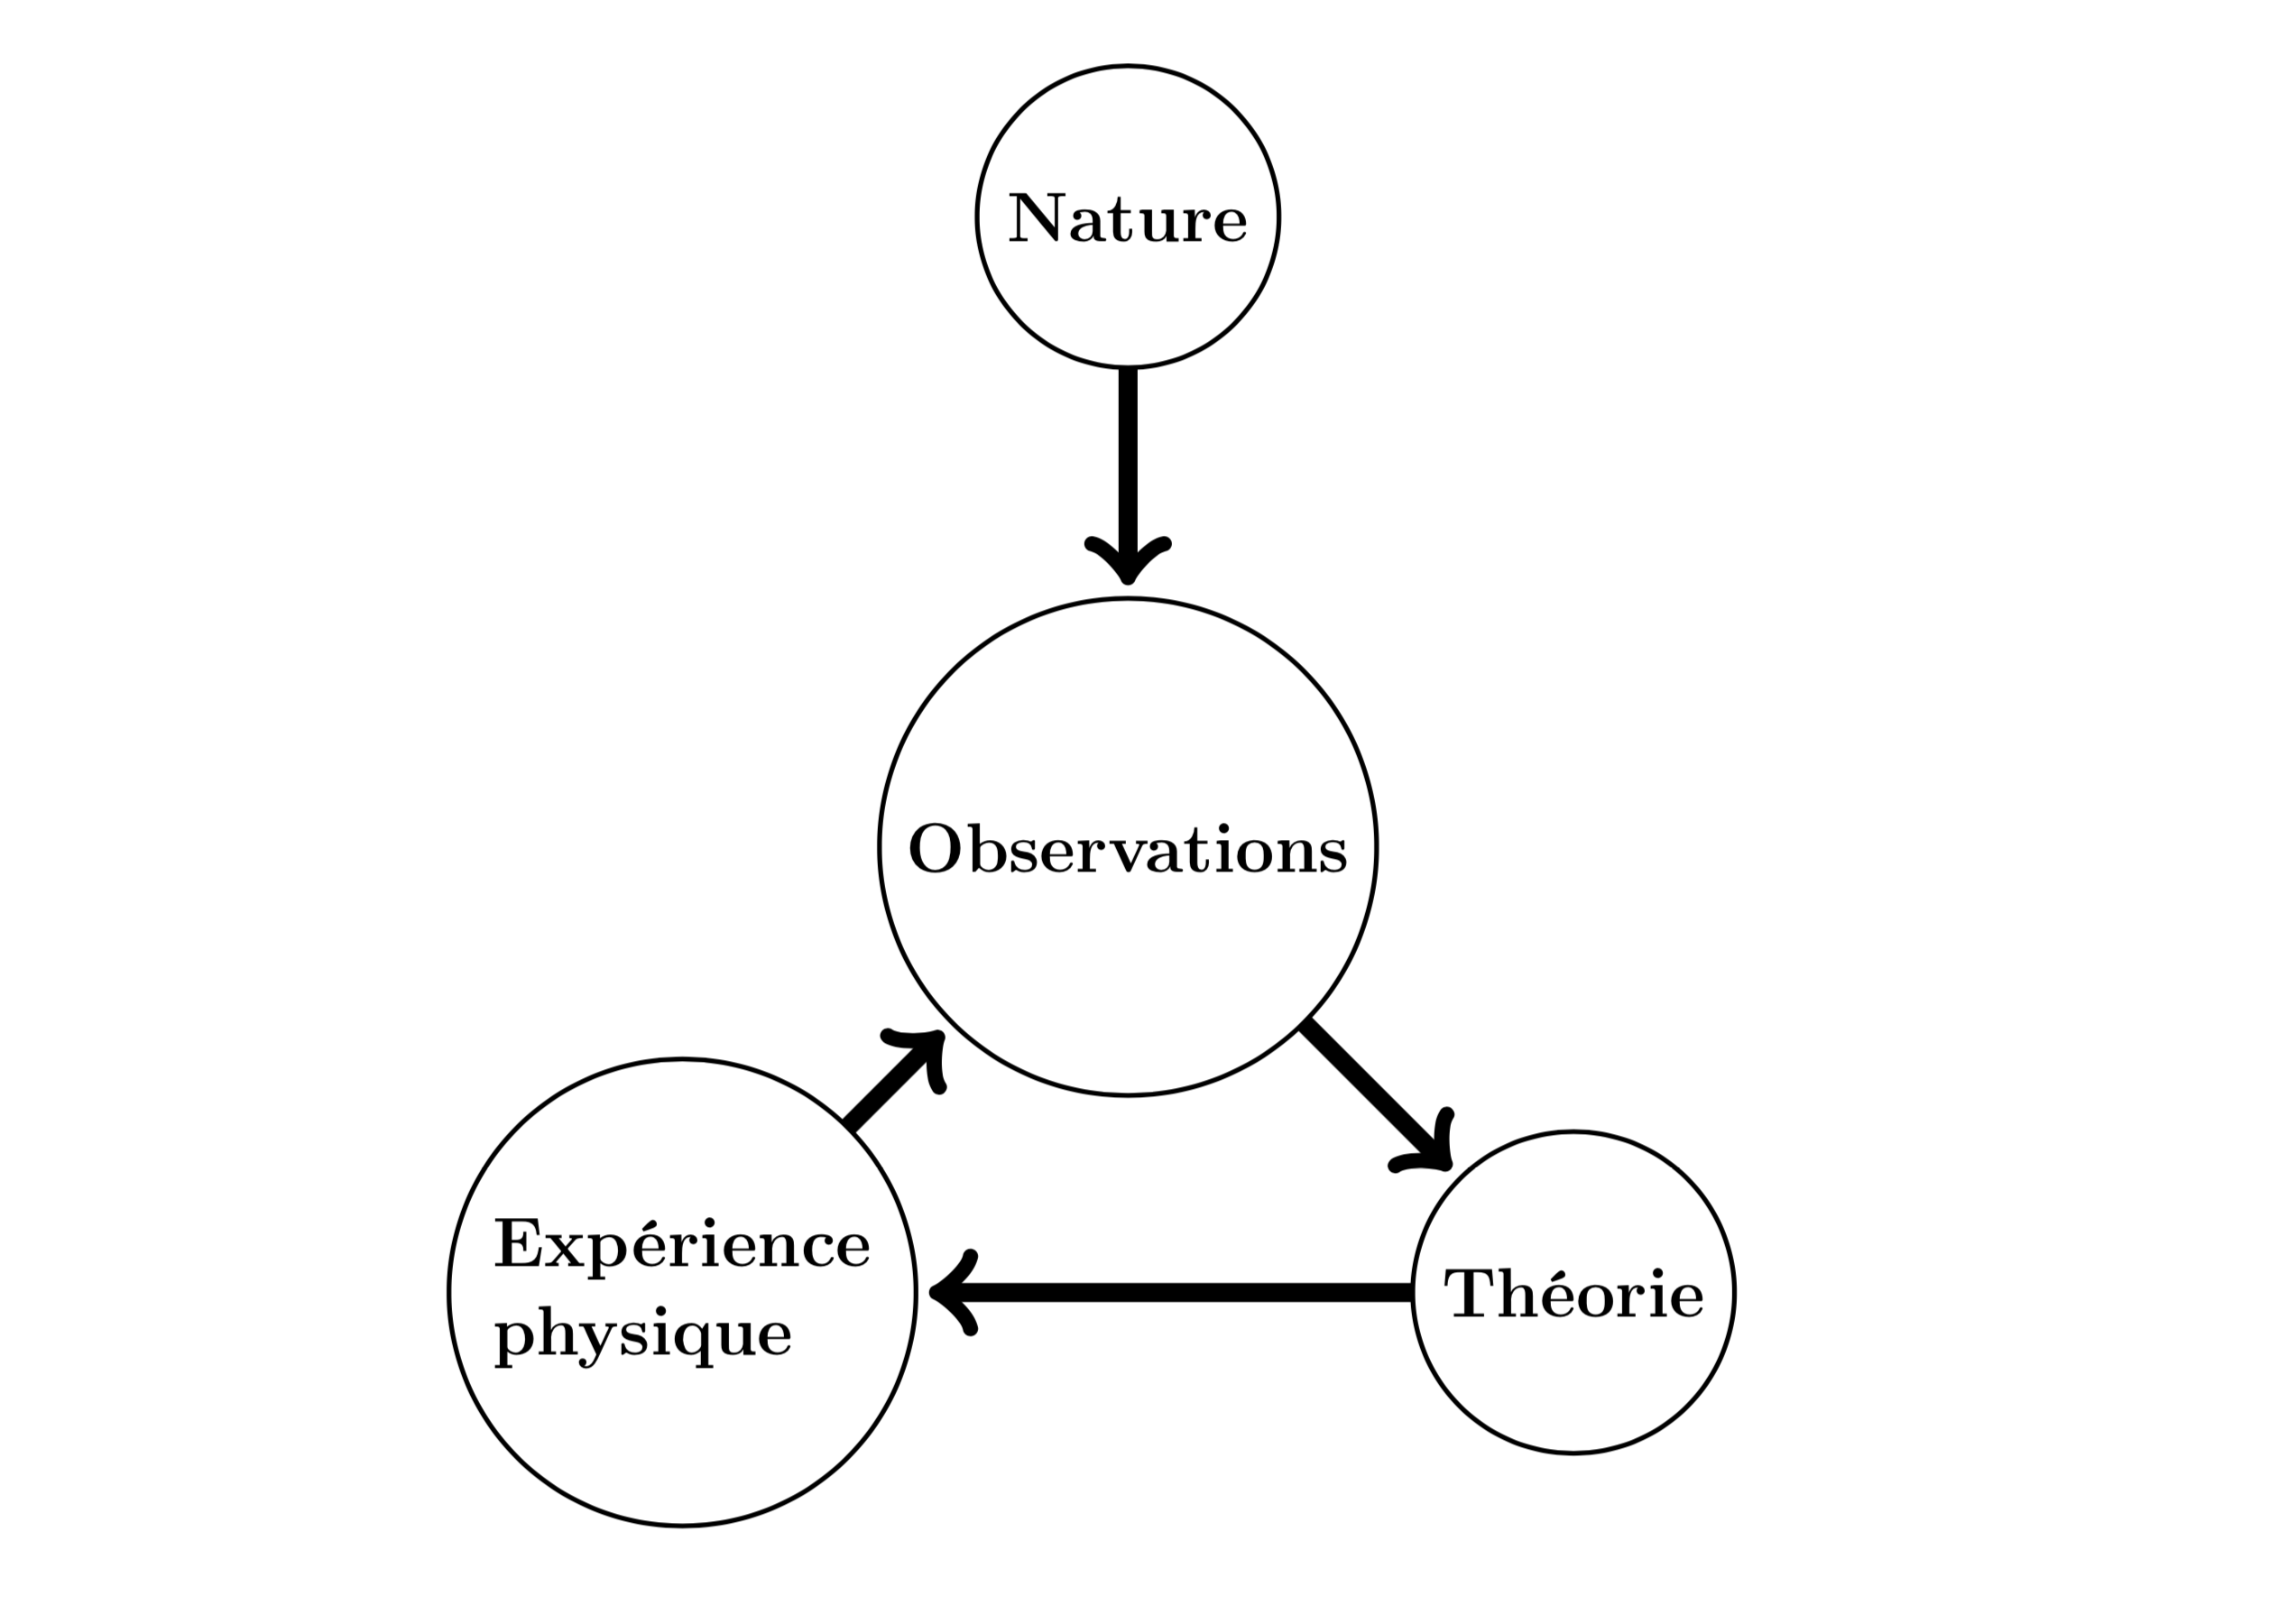
\includegraphics[width=\linewidth]{images/edl_simu_old.png}
            \caption{\label{fig:edl_simu_old}Les expériences physiques permettent de valider les théories.}
        \end{subfigure}\hfill
        \begin{subfigure}[t]{0.48\textwidth}
            \centering
            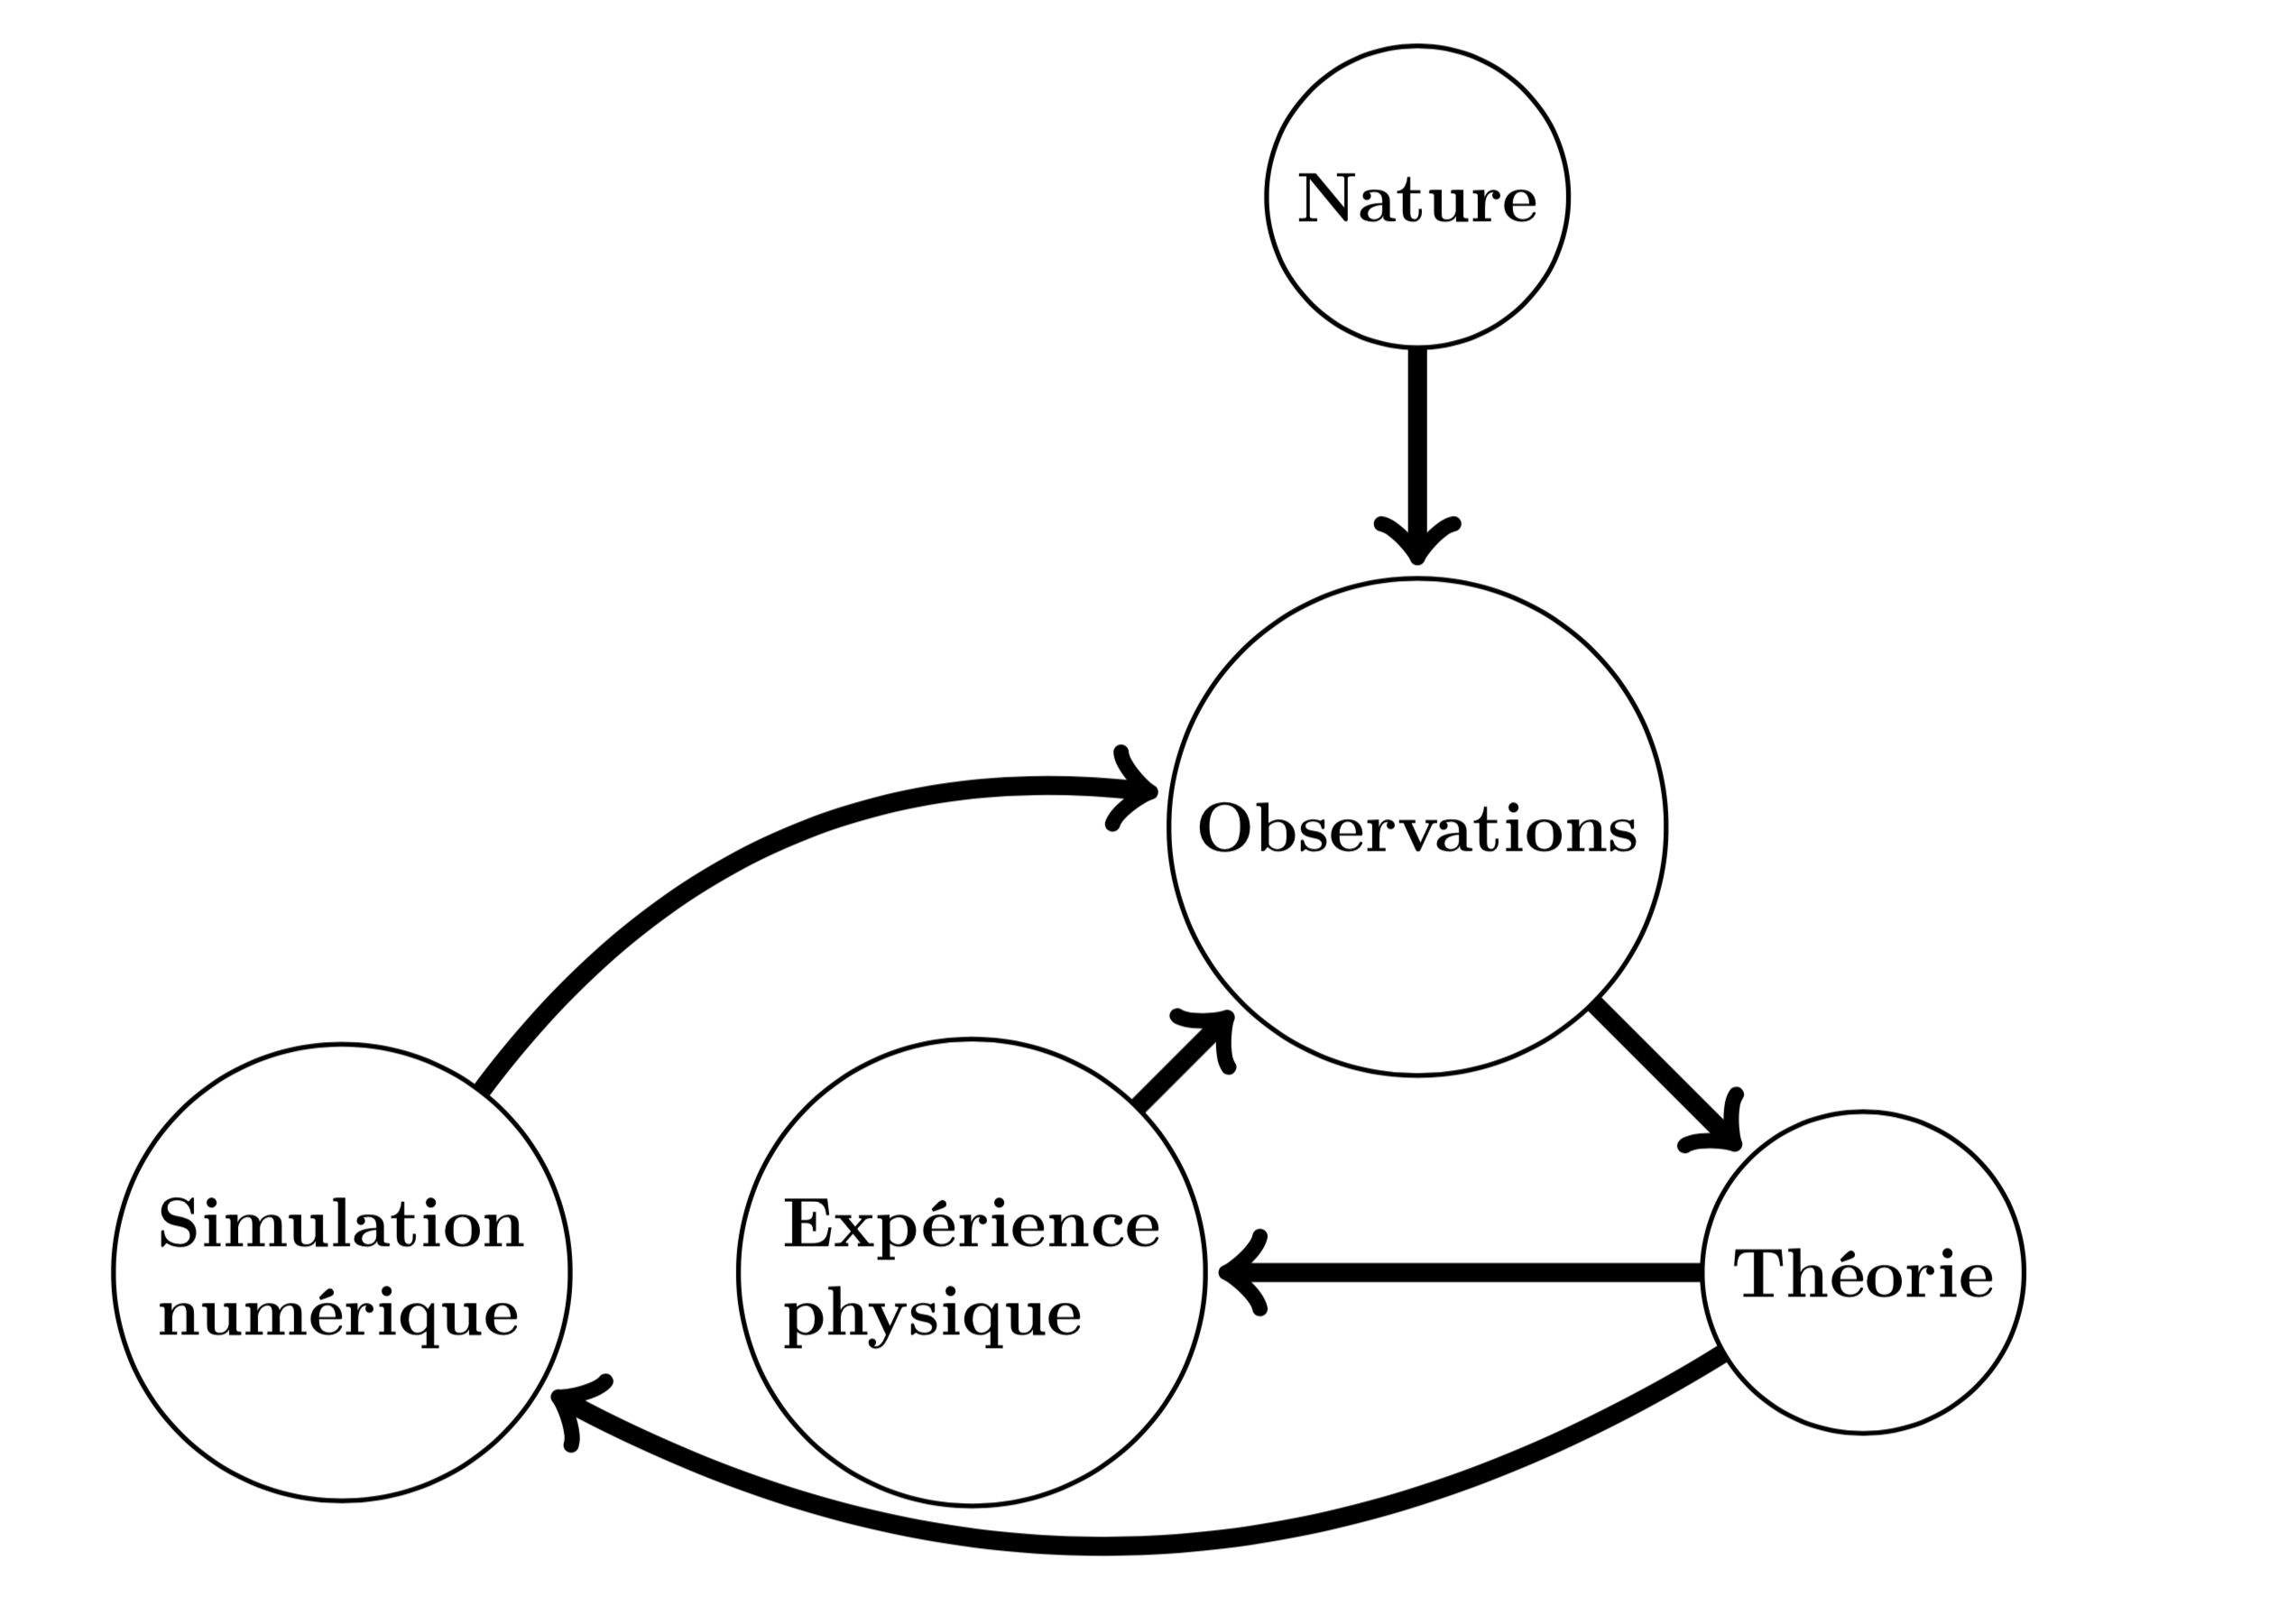
\includegraphics[width=\linewidth]{images/edl_simu_new.png}
            \caption{\label{fig:edl_simu_new}La simulation numérique peut être une alternative aux expériences physiques.}
        \end{subfigure}
        \caption{La simulation numérique a apporté une nouvelle façon d'expérimenter les théories.}
        \label{fig:tikz_simulation}
    \end{figure}
    

      
    %TikZ picture
%\begin{figure}
%\begin{center}
%\begin{minipage}[]{.5\textwidth}
%\begin{tikzpicture}[->,shorten >=1pt,auto,node distance=3.8cm,   scale=0.49, every %node/.style={transform shape}]
%\tikzstyle{every state}=[fill=none,draw=black,text=black,  , font=\bf]
%\tikzstyle{edge_style} = [draw=black, line width=2, ultra thick]
%\tikzstyle{node_style} = [circle,draw=blue,fill=blue!20!,font=\sffamily\Large\bfseries]
%\node[state]					    (A)                     {Nature};
%\node[state]        				(B) [below of=A]        {Observations};
%\node[state,]         		    (D) [below right of=B]  {Théorie};
%\node[state, align=left]         	(C) [below left of=B]   {Expérience\\ physique};
%\path
%(A) edge [edge_style]   node {} (B)
%(B) edge [edge_style]   node {} (D)
%(C) edge [edge_style]   node {} (B)
%(D) edge [edge_style]   node {} (C);
%\end{tikzpicture}
%\end{minipage}%
%\begin{minipage}[]{.5\textwidth}
%\begin{tikzpicture}[->,shorten >=1pt,auto,node distance=3.8cm,   scale=0.49, every %node/.style={transform shape}]
%\tikzstyle{every state}=[fill=none,draw=black,text=black,  , font=\bf]
%\tikzstyle{edge_style} = [draw=black, line width=2, ultra thick]
%\tikzstyle{node_style} = [circle,draw=blue,fill=blue!20!,font=\sffamily\Large\bfseries]
%\node[state]					(A)                    {Nature};
%\node[state]        					(B) [below of=A] {Observations};
%\node[state,]         					(D) [below right of=B] {Théorie};
%\node[state, align=left]         	(C) [below left of=B] {Expérience\\ physique};
%\node[state, align=left]        	(E) [left of=C]       {Simulation\\numérique};
%\path
%(A) edge [edge_style]            node {} (B)
%(B) edge [edge_style]     node {} (D)
%(C) edge [edge_style]           node {} (B)
%(D) edge [edge_style]             node {} (C)
%edge [edge_style, bend left]     node {} (E)
%(E) edge [edge_style, bend left]  node {} (B);
%\end{tikzpicture}
%\end{minipage}
%\end{center}
%\caption{La simulation numérique a apporté une nouvelle façon d'expérimenter les théories.} 
%\label{fig:tikz_simulation}
%\end{figure} 
     
    
     
    \subsubsection{Principe de la simulation numérique}
    %%%%%%%%%%%%%%%%%%%%%%%%%%%%%%%%%%%%%%%%%%%%%%%%
    
        La majorité des simulations numériques sont basées sur des équations dites \textit{gouvernantes} et qui sont des approximations des phénomènes étudiés. Ces équations ont besoin d'être discrétisées pour pouvoir être exécutées par un ordinateur. En mathématiques, la discrétisation est un procédé qui permet de passer d'un modèle à son équivalent discret. Ce procédé ne permet pas de décrire le phénomène réel, mais de l'approcher avec plus ou moins d'erreurs. Pour améliorer ces simulations, ces représentations doivent utiliser des maillages les plus fins possible (voir \autoref{pic_maillage}). Une autre approche utilise des modèles probabilistes pour représenter un comportement. Elle est adaptée pour des phénomènes où chaque élément peut subir différents événements. Pour chaque étape du calcul, le résultat évolue grâce à des tirages aléatoires (méthode de Monte-Carlo \cite{Kroese2014}). Pour améliorer la précision des simulations, il est donc nécessaire d'augmenter le nombre de tirages et donc le nombre de calculs à réaliser.
        Que ce soit pour affiner la taille des maillages ou augmenter le nombre de tirages, les simulations numériques nécessitent de grandes puissances de calculs. 
            
            \begin{figure}
            \center
            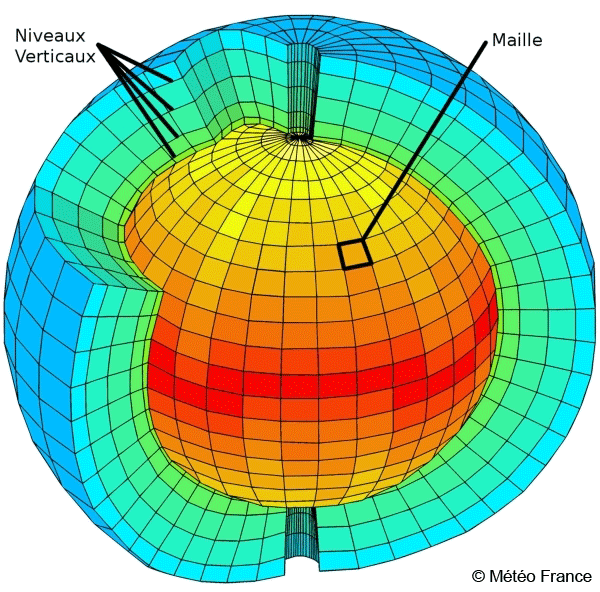
\includegraphics[width=5cm]{images/Chapitre1/maillage.png}
            \caption{\label{pic_maillage} Le maillage le plus fin exploité par Météo-France pour ses prévisions régionales restitue des mailles de 2,5 km de côté (source \url{www.irma-grenoble.com}).}
            \end{figure}

    
    \subsubsection{Quelques applications de simulations numériques}
    %%%%%%%%%%%%%%%%%%%%%%%%%%%%%%%%%%%%%%%%%%%%%%%%
        Lorsque l'on évoque la simulation numérique, on pense souvent aux domaines physiques (météorologie, mécanique, biologie), mais elle peut aussi être utilisée en sciences humaines (sociologie, analyse démographique) ou dans le domaine de la sécurité nationale. En effet, Alan Turing a développé les premiers ordinateurs lors de la fin de la Deuxième Guerre mondiale pour aider au décryptage des messages allemands. En 1936, il avait présenté les premiers concepts de programmes et donné naissance à l'aide d'une expérience de pensée à l'ancêtre des ordinateurs nommée machine de Turing. L'utilisation de simulations numériques a de nombreux avantages. En plus de profiter de la puissance de calculs des ordinateurs, elle permet de simuler des phénomènes dont les conditions ne sont pas reproductibles sur terre (physique théorique). Un autre avantage est de réduire drastiquement les coûts d'une expérience, par exemple pour la réalisation de crash automobile, où ce ne sont plus de réels modèles de voiture, mais bien des voitures virtuelles qui sont crashées sur des murs.
        
        Dans le domaine de la santé, l'étude de la structure des protéines est primordiale.  Ces molécules qui assurent les fonctions élémentaires d'une cellule interviennent dans la majorité des processus biologiques (régulation du métabolisme, défense immunitaire). Dans ce genre de simulation, le pas de temps est de l'ordre de la nanoseconde. Grâce à la simulation numérique, une meilleure compréhension de ces molécules permet la découverte de nouveaux médicaments ou antibiotiques. 
        Aussi, des modélisations peuvent être utilisées pour analyser la propagation d'un virus comme la grippe aviaire à l'échelle mondiale pour mieux protéger les populations\cite{CEA2007}. En février 2020, le gouvernement français indiquait travailler sur la modélisation de la propagation du COVID-19\footnote{\url{https://www.gouvernement.fr/info-coronavirus}} (coronavirus). Cette modélisation fait intervenir plusieurs paramètres comme le lieu et la période d'incubation du virus ou encore la fréquentation et les destinations des passagers des 4000 principaux aéroports mondiaux. En mars 2020, le supercalculateur le plus puissant au monde (Summit) était utilisé pour identifier 77 molécules potentiellement efficaces contre le COVID-19 \cite{Smith2020}.

        En astrophysique, la simulation numérique est aussi capitale du fait de la non-reproductibilité des expériences en laboratoire.  À l'opposé de l'exemple précédent sur les protéines, elle permet d'étudier des objets aussi grands que complexes comme le système solaire, les galaxies ou bien l'univers. La simulation permet alors de faire évoluer le système avec un pas de temps allant jusqu'au million d'années. Une équipe du CEA a pu reconstituer le passé de la galaxie Andromède en analysant les observations réalisées grâce au satellite infrarouge Spitzer\cite{Block2006}. Après avoir mis au point le modèle adéquat et après plusieurs heures de simulation, ils ont pu déterminer qu'elle avait été percutée par une galaxie voisine il y a plus de 210 millions d'années et que sa forme actuelle résultait de cet impact (voir\autoref{pic:cea_galaxy}).
    
        
        \begin{figure}
            \center
            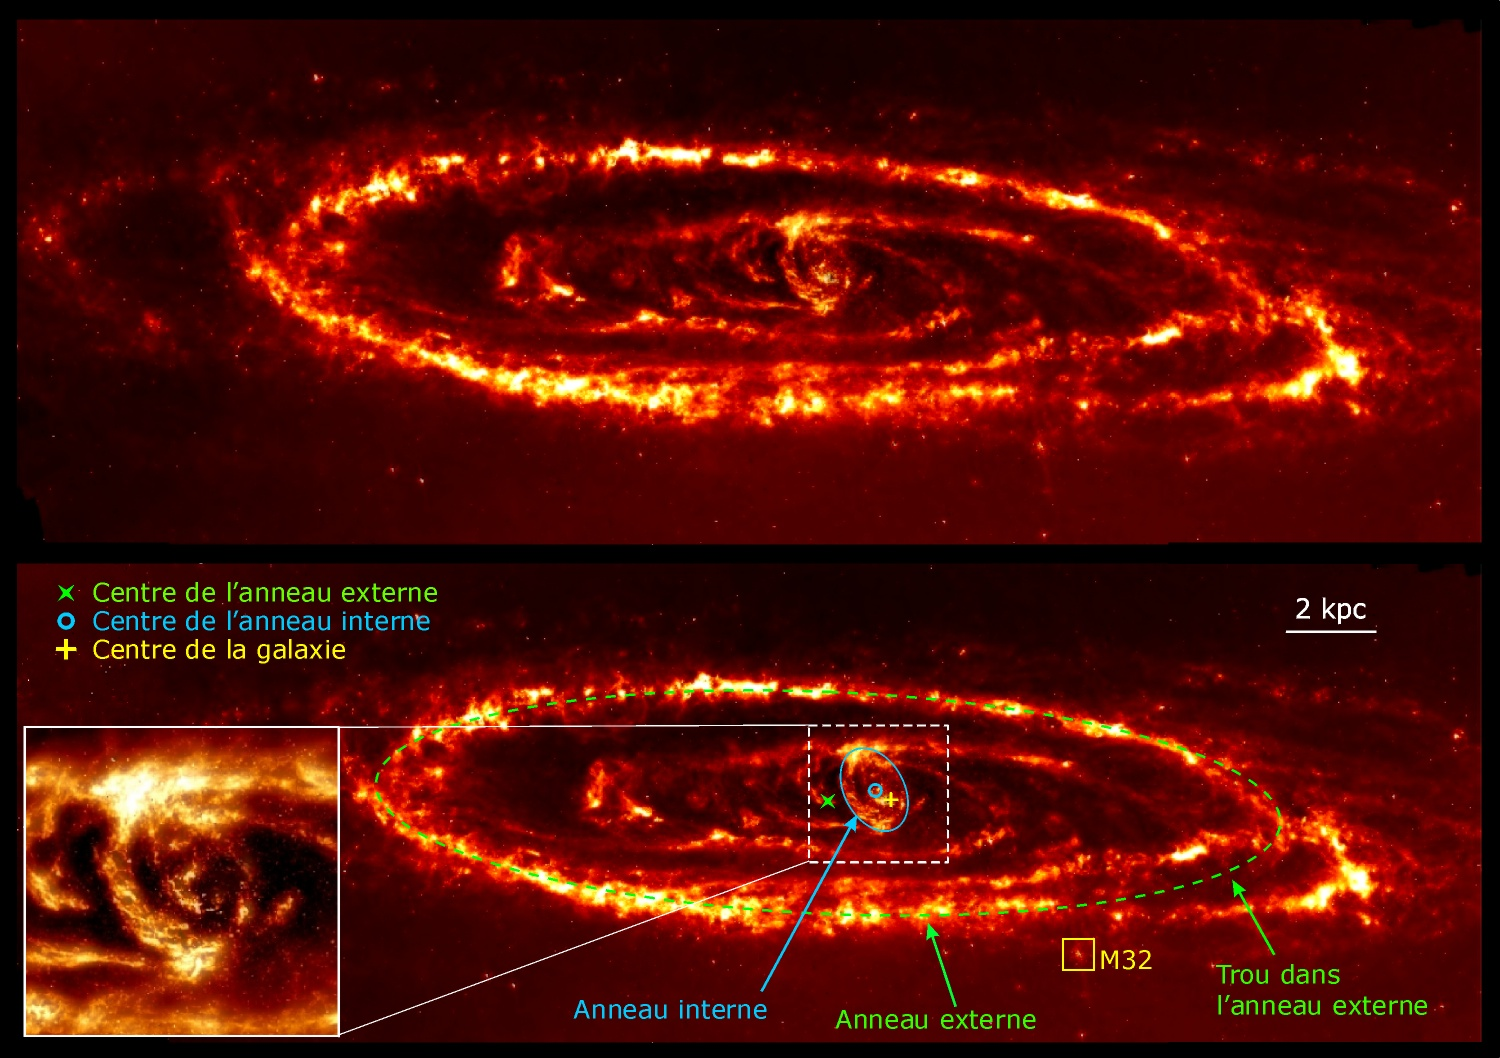
\includegraphics[width=12cm]{images/cea_galaxy.jpg}
            \caption{\label{pic:cea_galaxy} Cartographie de l'émission infrarouge des poussières  obtenues à l'aide du satellite Spitzer\protect\footnotemark. En bas : identification de la structure en double-anneau décentré et agrandissement de l'anneau interne. À la distance de M31, l'anneau interne a une dimension de 3 par 4.5 milliers d'années-lumière.}
        \end{figure}
        \footnotetext{\url{http://irfu.cea.fr/Phocea/Vie_des_labos/Ast/ast.php?id_ast=958&t=actu}}

        Pour la compétitivité et l'innovation des entreprises, les simulations numériques sont désormais un outil indispensable. Cet outil les aide à la conception, à la décision et au contrôle de leurs activités. 
        Dans l'industrie des hydrocarbures, la recherche pétrolière est très coûteuse : le coût d'un forage d'exploration maritime peut atteindre 100 millions d'euros\footnote{\url{https://www.planete-energies.com/fr/medias/decryptages/la-difficile-decision-de-lancer-un-forage}}.  Les pétroliers utilisent la simulation numérique pour analyser les fonds marins, modéliser les réservoirs de pétrole et, in fine, optimiser l'extraction du pétrole. Pour cela, ils utilisent des bateaux tractant d'immenses lignes flottantes pourvues de capteurs. Le principe est d'émettre des explosions, et d'analyser le réfléchissement des signaux sur le fond marin (voir \autoref{pic:hpl_petrole}). Grâce à l'analyse de ces données, il est alors possible de construire une cartographie du fond marin et ainsi déceler la présence ou non de réservoirs d'hydrocarbures.  En perçant le puits de façon optimale, il sera d'autant mieux exploité. De plus, le risque de forer au mauvais endroit est lui aussi diminué. Actuellement, le taux de succès est de deux forages sur trois.

        \begin{figure}
            \center
            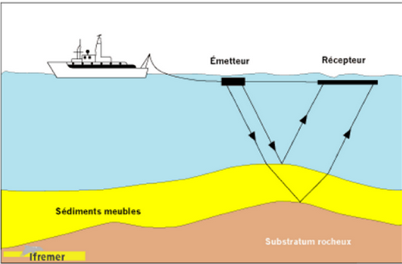
\includegraphics[width=8cm]{images/hpl_petrole.png}
            \caption{\label{pic:hpl_petrole}Étude de fond marin grâce à la sismique de réflexion.}
        \end{figure}


\subsection{Le calcul haute performance} \label{sec:supercomputer}
%%%%%%%%%%%%%%%%%%%%%%%%%%%%%%%%%%%%%%%%%%%%%%%%%%%%%%%%%%%%%%
        
        
    Aujourd'hui, presque que tout ce que nous utilisons a été simulé, à un tel point que l’avancée de nos sociétés dépend de la puissance de calcul disponible pour réaliser ces simulations. La rapidité de l'exécution des simulations numériques dépend alors de la puissance de calcul disponible pour exécuter l’application. Le domaine du \gls{hpc} est le domaine informatique qui consiste à exécuter ces applications le plus efficacement possible sur une plateforme. Celle-ci peut être un simple ordinateur personnel ou un centre de calculs dédié. De telles infrastructures sont utilisées dans de nombreux domaines dont les principaux sont la simulation numérique, la cryptographie, l'analyse de données (\textit{big data}), l’intelligence artificielle ou la sécurité. En fonction des besoins des applications (puissance de calcul, espace mémoire, stockage), mais aussi des budgets alloués, des infrastructures adaptées sont développées:
    
   \begin{enumerate}
        \item \textbf{Le supercalculateur dédié} (\textit{dedicated supercomputer}) consiste à la création d'une architecture unique qui ne sera pas répliquée. Le premier supercalculateur élaboré par Seymour Cray alors employé de l'entreprise Control Data (le CDC6600) utilisait un tel mode de conception. Il était alors l'ordinateur le plus puissant de la planète grâce à une mémoire de 131000 mots de 60 bits, une fréquence de 40 MHz et sa capacité calculatoire de $3.3 \times 10^6$ opérations par seconde. À titre de comparaison, l'ordinateur portable utilisé pour écrire ce manuscrit est capable d'exécuter plus de $10^9$ opérations par seconde. L'objectif de ce type d'infrastructure est d'être parfaitement adapté aux besoins de l'application. La conception de ces architectures étant unique, les frais de conception sont très élevés, mais cette spécificité en fait des architectures très performantes. 
        
        \item \textbf{Le commodity cluster}. L'augmentation de la vitesse des circuits ainsi que l'augmentation exponentielle du nombre de transistors des circuits a rendu les supercalculateurs dédiés très difficiles à alimenter en énergie ou à être refroidi. Il a alors fallu repenser leur architecture pour continuer à augmenter la puissance des supercalculateurs. Les \textit{commodity cluster} agrègent du matériel grand public (haut de gamme) pour former des grappes de calculs de plusieurs milliers de processeurs. La performance de ces architectures ne repose pas sur l'utilisation de matériels ultra-optimisés, mais sur l'agrégation de milliers de serveurs (noeuds de calculs) travaillant ensemble. L'Intel Paragon est un des premiers exemples de cluster construit par Intel en 1992\footnote{source: \url{https://www.top500.org/featured/systems/intel-xps-140-paragon-sandia-national-labs/\#Historical}}, qui regroupe 3680 processeurs indépendants atteignant une puissance cumulée de $143.40 \times 10^9$ \gls{FLOP}. Ce modèle de supercalculateur est le plus répandu actuellement et a permis l'élaboration des supercalculateurs les plus puissants de la planète. Ces infrastructures sont généralement développées pour des industries privées ou de grandes universités (voir \autoref{fig:hpc_bsc_super}).
        
        \item \textbf{L'informatique en nuage} (\textit{cloud computing}),  utilise le modèle \textit{System as a Service} (SAS) pour apporter aux entreprises manquant de moyens, ou de compétences, un accès à une infrastructure HPC externalisée. Les principaux avantages sont la flexibilité d'usage (adapter l'infrastructure à son besoin) ainsi que la sous-traitance de la gestion de la plateforme. L'informatique en nuage permet  à des petites structures (PME, petites universités) d'avoir accès à une ressource de calculs facilement à coûts modérés. Nous pouvons notamment citer le projet SIMSEO \cite{Saguez2016} qui a pour but de sensibiliser et d'accompagner les PME à utiliser la simulation numérique. %L'informatique en nuage permet aussi de faciliter les évolutions de matériels et permet d'utiliser les dernières technologies.
        %Le \textit{nuage} peut être implémenté de deux façons. La première est d'utiliser un nuage public où les machines sont gérées par le prestataire directement dans leur centre de données. La deuxième est d'installer un \textit{nuage} privé, le client choisi où installer la plateforme. Cette seconde solution est particulièrement recherchée par les entreprises utilisant des données sensibles et refusant qu'elles soient stockées dans un autre pays. 
        
        \item \textbf{Les grilles informatiques} (\textit{Grid Computing}) sont un regroupement de ressources informatiques à grande échelle (nationale voire internationale). Par exemple \textit{Einstein@Home} \cite{Abbott2009} est un projet de recherche mondial sur les ondes gravitationnelles  qui regroupe les ordinateurs de 50000 utilisateurs connectés à travers le monde pour analyser les données transcrites par des capteurs. En octobre 2000, l'université de Stanford a déployé un projet de calcul distribué, nommé Folding@Home \cite{Larson2009}, permettant simuler la dynamique des protéines (pliage et mouvement) impliquées dans une grande variété de maladies. Pour contribuer aux calculs, il est possible d'installer un logiciel sur son ordinateur qui effectue les calculs lorsque ce dernier n'est pas utilisé. En avril 2020, alors plus de la moitié de la population est confinée chez elle à cause de l'épidémie du COVID-19, la puissance de calcul du projet Folding@Home est utilisée pour étudier le coronavirus SARS-CoV-2 et aider au développement d'un vaccin\footnote{Coronavirus : comment votre ordinateur pourrait aider à trouver un vaccin - \url{https://www.ft.com/video/51bc9532-b08d-4129-b4db-c88ca5d42342}}. Le réseau compte plus de 2 millions de processeurs et  700 000 GPU, formant la plateforme de calcul la plus puissante de la planète ($2,5 \times 10^{18}$ opérations par seconde). 
        
    \end{enumerate}
        
        
        \begin{figure}
        \center
        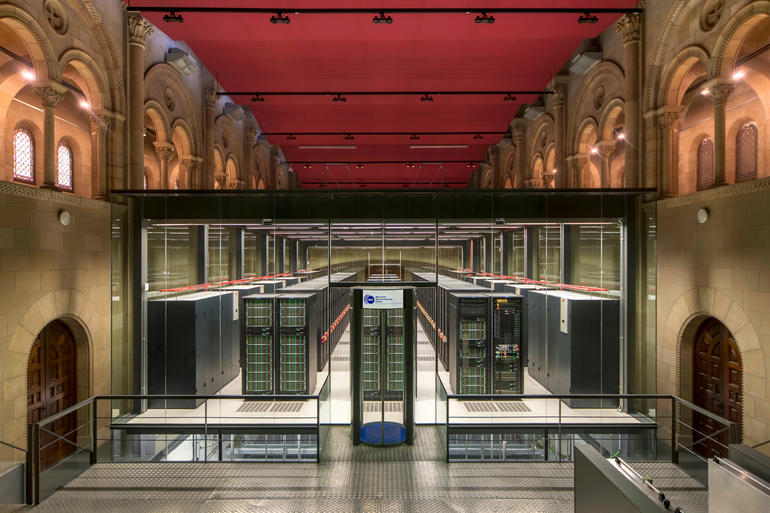
\includegraphics[width=12cm]{images/hpc_bsc_super.jpg}
        \caption{\label{fig:hpc_bsc_super} Le supercalculateur du Centre de Calcul de Barcelone (BSC) est installé dans une ancienne chapelle.}
        \end{figure}
        
        
    
        
    \subsubsection{Architecture des supercalculateurs}
    %%%%%%%%%%%%%%%%%%%%%%%%%%%%%%%%%%%%%%%%%%%%%%
    
        Les deux principales caractéristiques d'un supercalculateur sont sa capacité à calculer rapidement ainsi que sa capacité à mémoriser les informations et les résultats produits. L'architecture des supercalculateurs modernes n'est pas très différente de celle des ordinateurs classiques. La puissance d'une telle plateforme vient seulement de l'agrégation de centaines de ressources de calculs, capables de travailler ensemble pour résoudre un problème complexe. Le domaine du HPC consiste à exécuter efficacement des applications sur de telles architectures. Pour cela, l'infrastructure utilisée doit gérer l'équilibrage de la charge de calcul sur les différentes ressources disponibles ainsi que la gestion des communications entre les ressources. Un supercalculateur moderne possède généralement les cinq parties suivantes:
      
        \begin{enumerate}
        
            \item \textbf{Les serveurs} utilisés dans un supercalculateur possèdent un ou plusieurs processeurs. Comme un ordinateur classique, chaque processeur est relié à la mémoire et au stockage (voir \autoref{fig:motherboard}). En fonction des configurations, chaque serveur peut être agrémenté d'un ou plusieurs accélérateurs (GPU). La principale différence avec un ordinateur classique, autre que la puissance des matériels utilisés, vient du système d'interconnexion (voir \autoref{fig:dl360_back}). Les serveurs doivent pouvoir échanger des informations pour se synchroniser ou partager des résultats entre eux et accéder au stockage (voir \autoref{sec:edl_interco}).
        
                \begin{figure}[t!]
                    \centering
                    \begin{subfigure}[t]{0.48\textwidth}
                        \centering
                        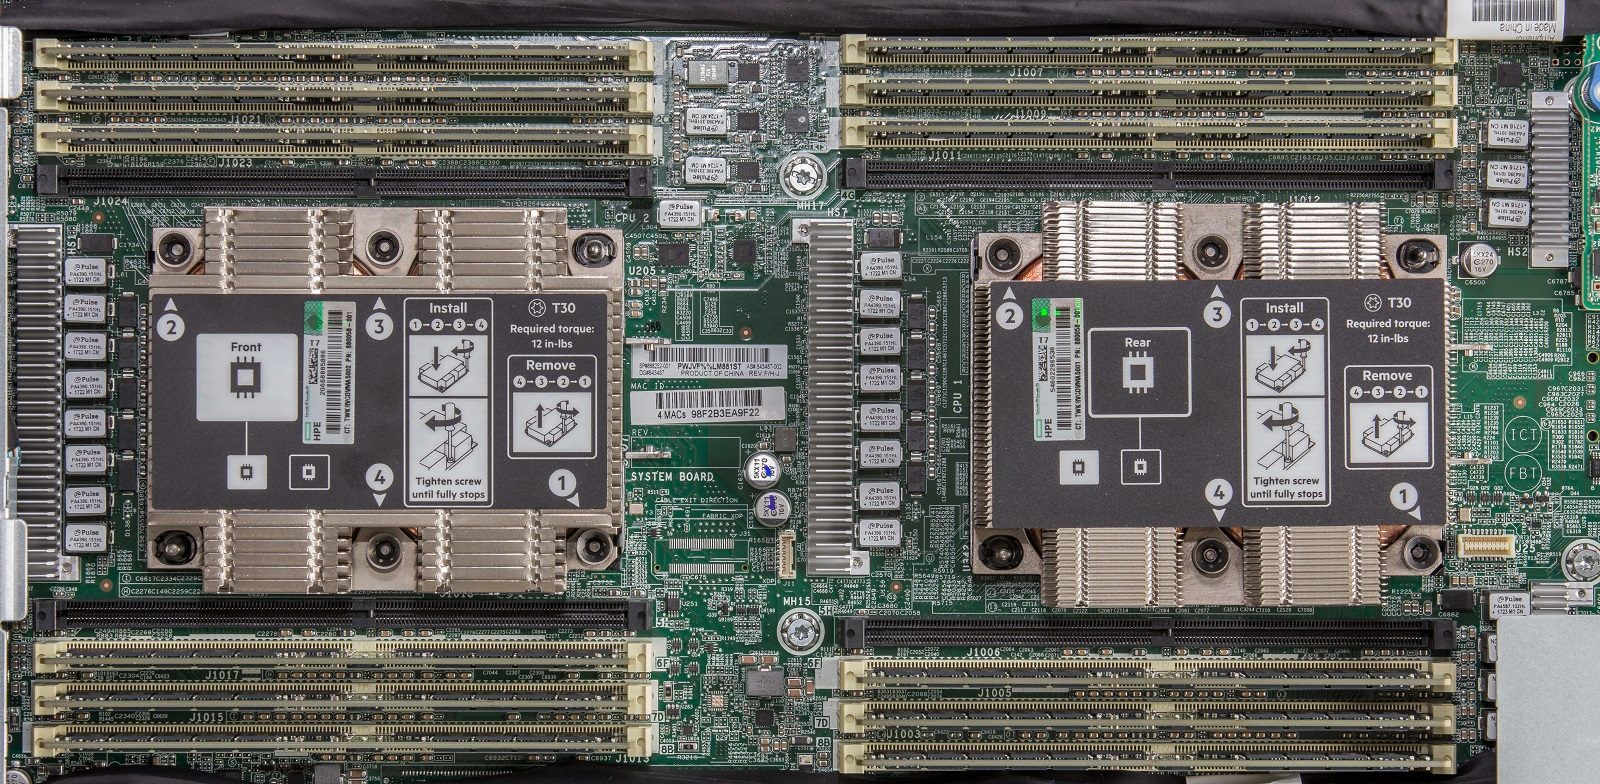
\includegraphics[width=.9\linewidth]{images/motherboard.jpg}
                        \caption{\label{fig:motherboard}Carte mère d'un serveur possédant deux processeurs.}
                    \end{subfigure}\hfill
                \begin{subfigure}[t]{0.48\textwidth}
                        \centering
                        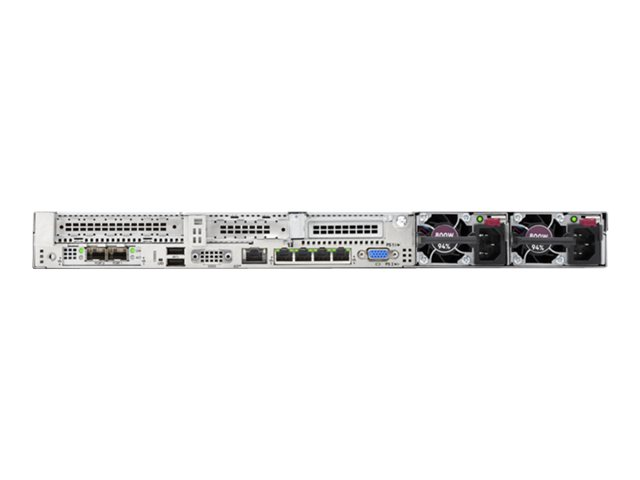
\includegraphics[width=\linewidth]{images/dl360_back.jpg}
                        \caption{Vu arrière d'un serveur exposant les différentes interfaces de connexion.\label{fig:dl360_back}}
                    \end{subfigure}
                    \caption{Exemple d'un serveur utilisé dans les supercalculateurs.}
                    \label{pic_pi_rect}
                \end{figure}
    
            \item \textbf{Les accélérateurs}. Un principe fondamental des processeurs énoncés par Von Neumann était leur universalité. Leur faculté à exécuter tout type de code est à la fois une force, mais aussi une de leur plus grande faiblesse. Ils sont très peu efficaces, en temps et en énergie, pour résoudre certains types de calculs tels que les traitements de signaux ou d'objets géométriques. Pour accélérer certaines classes d'applications, des architectures spécialisées, appelées accélérateurs, sont utilisés pour améliorer la performance et la consommation énergétique des infrastructures. Les applications d'intelligence artificielle utilisent des \gls{GPU} pour accélérer l'entraînement des modèles. D'autres accélérateurs comme les \gls{FPGA} peuvent être utilisés pour accélérer la phase d'inférence.
            
            :
                \begin{itemize}
    
                    \item\textbf{Les GPU}. À l'origine, les \gls{GPU} étaient destinés au domaine des jeux vidéo et aux calculs de rendus graphiques. Suite à leur utilisation pour d'autres applications que le rendu graphique, ces accélérateurs sont aussi nommés GP-GPU pour \textit{general purpose GPU}. À l'inverse des processeurs, les GPU sont composés de nombreux coeurs (plusieurs centaines). Ceux-ci sont moins complexes et performants que les coeurs de processeur, mais leur nombre les rend particulièrement efficaces pour certaines applications. La \autoref{fig:CPUvsGPU} compare l'évolution des performances des GPU avec celles des CPU de même génération. On remarque l'écart significatif séparant leur performance. Cependant, la figure représente la performance théorique des architectures et il est rare que les applications s'en approchent. 
                    Actuellement, il existe deux fournisseurs principaux de GPU (Nvidia et AMD) qui ont pu bénéficier de leur longue expérience dans le domaine du jeu vidéo. La première nécessite l'utilisation de langage propriétaire (\verb|CUDA|) quand la deuxième peut être programmée grâce au langage \verb|OpenCL|. Le principal avantage de \verb|CUDA| est de pouvoir utiliser des librairies optimisées par NVIDIA pour ses plateformes pour différents domaines (algèbre linéaire (cuBLAS, CUSPARSE), analyse de signal (cuFFT), apprentissage machine (cuDNN, TensorFlow). 
                    \verb|OpenCL| a été initié par Apple et est maintenant maintenu par le groupe Khronos. C'est un standard ouvert et libre de droits permettant l'exécution de codes sur différentes plateformes. Une application utilisant \verb|OpenCL| pourra être, en théorie, facilement portée sur d'autres architectures (CPU, FPGA, DSP). 
                    
                        \begin{figure}
                        \center
                        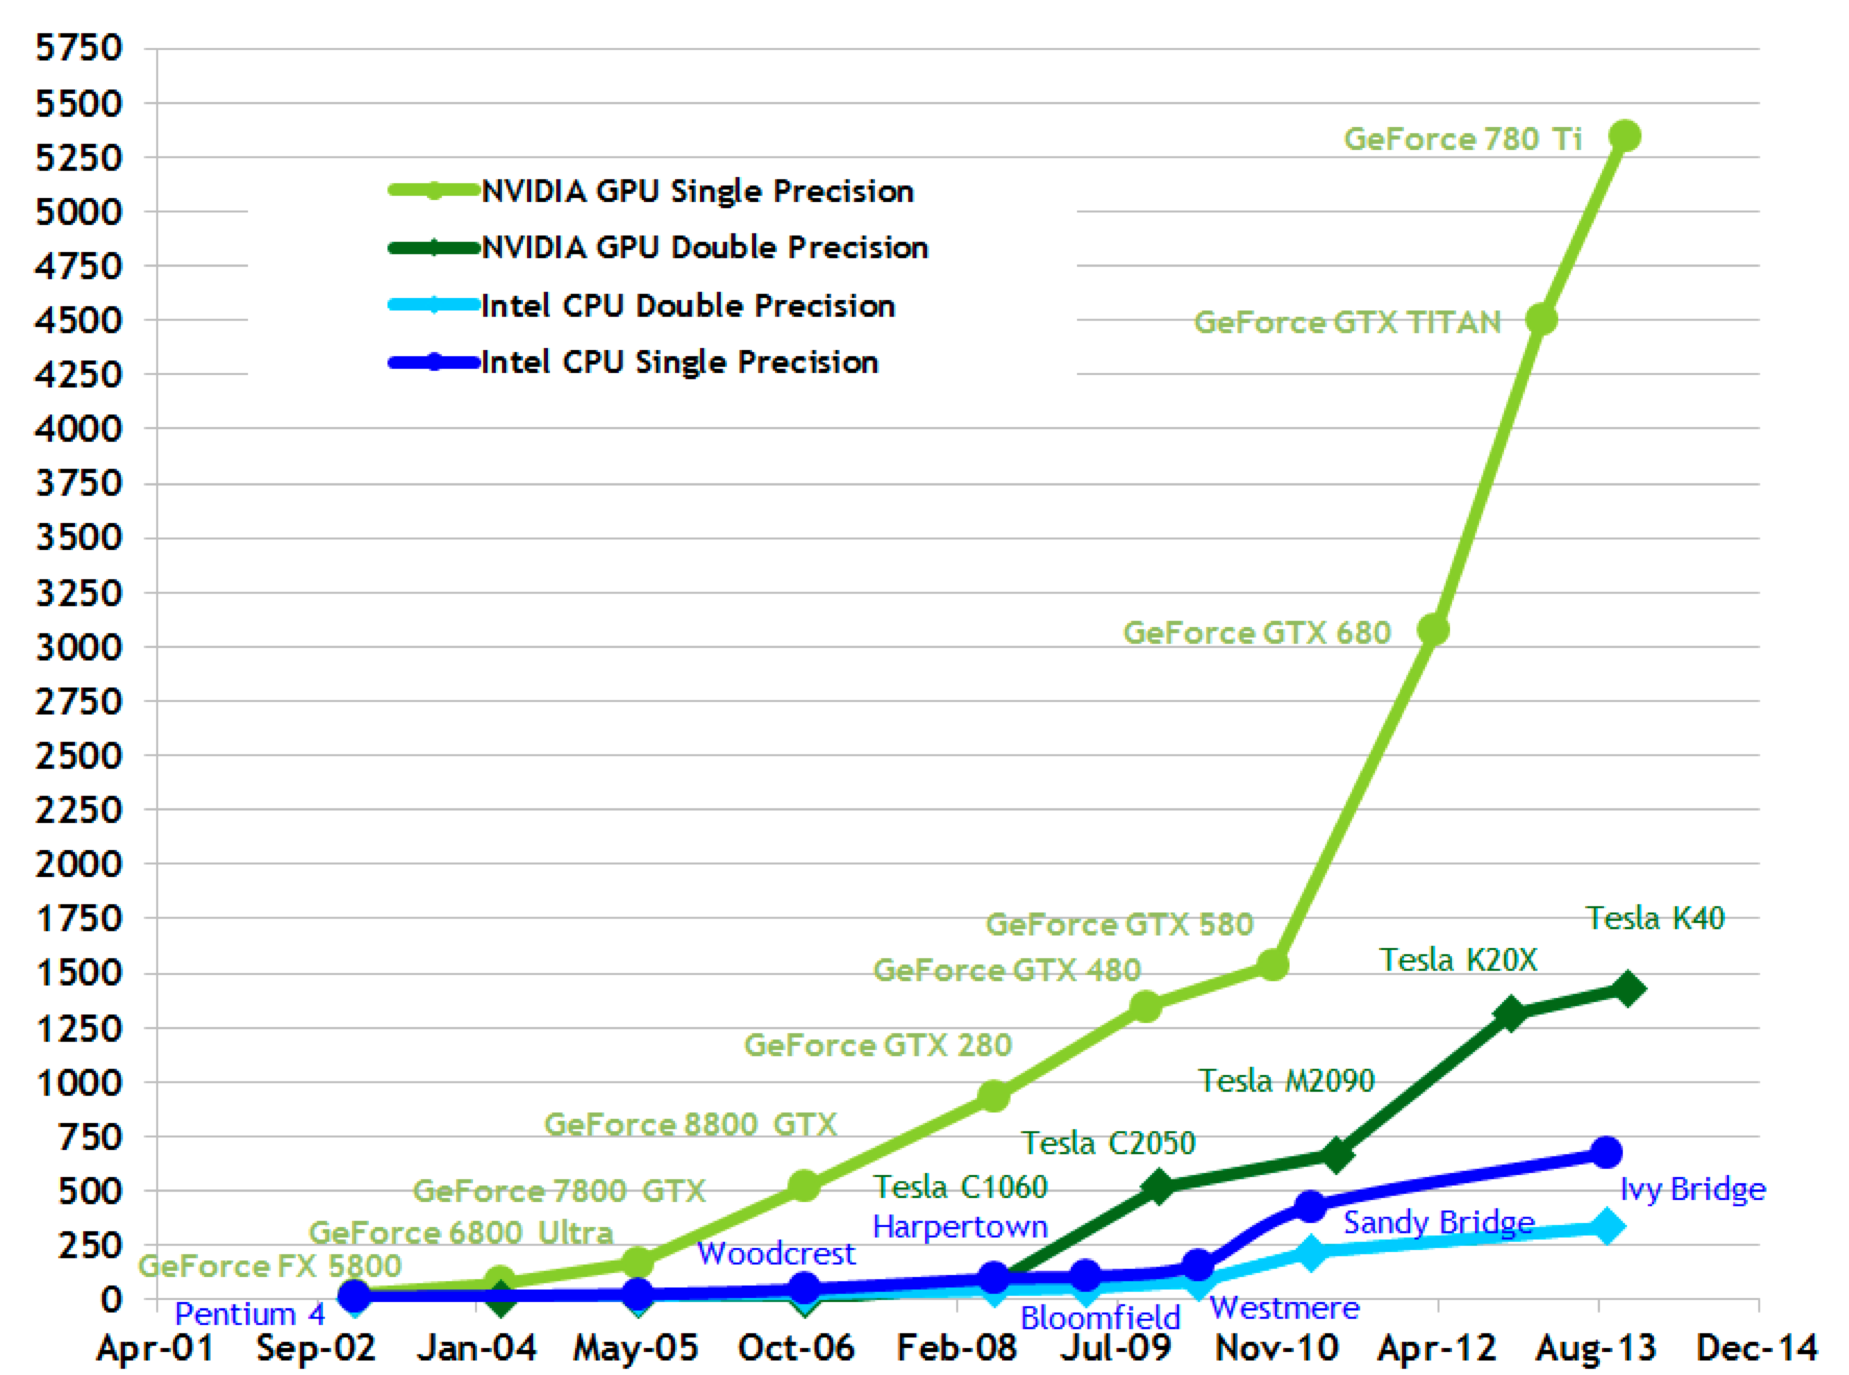
\includegraphics[width=10cm]{images/CPUvsGPU.png}
                        \caption{\label{fig:CPUvsGPU} Comparaison des performances entre différentes générations de CPU et de GPU}
                        \end{figure}
                     
                    
                    
                    
                    %Cependant, pour des applications particulièrement adaptées, le GPU n'a pas d'équivalent actuellement en termes de performance. La performance du bus mémoire d'un GPU est elle aussi bien supérieure, rendant ces architectures d'autant plus intéressantes pour les codes dont la performance est limitée par le système mémoire. 
                    
                    %Acutellement, le développement ou le portage d'applications pour pouvoir être exécutées sur ces architectures demande un investissement conséquent. L'architecture spécifique des GPU nécessite au programmeur de présenter explicitement la parallélisation d'un noyau. De plus, le GPU possédant son propre espace mémoire, le programmeur doit gérer explicitement les transferts entre celle-ci et la mémoire centrale du serveur.
                    %De nombreux travaux essaient de combler cette difficulté. La plus notable étant surement OpenACC. Crée en 2011, cet outil permet d'annoter le code source d'une application à l'aide de \verb|#pragma| pour indiquer au compilateur les zones parallélisable. Avec un effort raisonable, des performances proches des performances atteinte en utilisant \verb|CUDA| peuvent être atteinte. 
                        
                    \item\textbf{Les FPGA.}  Les \gls{FPGA} sont de simples circuits intégrés qui contiennent des portes logiques pouvant être programmées pour la réalisation d'un circuit. 
                    Les méthodes traditionnelles de développement sur FPGA nécessitent la conception d'une architecture matérielle utilisant un langage adapté comme le Hardware Description Language (HDL). Pour ce faire, le développeur doit concevoir les chemins de données ainsi que la logique de contrôle. Il s'agit d'un processus de développement fastidieux et complexe qui peut entraver leur adoption. Les FPGA les plus récents peuvent être programmés à l'aide d'\verb|OpenCL|.
                    Implémenter un circuit à l'aide d'un FPGA peut fournir une efficacité énergétique légèrement inférieure à celle obtenue par une implémentation d'un \gls{asic}. Cependant, le fait que les FPGA soient programmables leur donne un avantage sur les ASIC, car le même matériel peut être reprogrammé en un nouveau circuit. Le temps de reprogrammation étant relativement faible, il peut être intéressant de reprogrammer le FPGA plusieurs fois pour les différentes phases de l'application. Cependant, la complexité de programmation des FPGA et leur prix très élevé sont les principaux freins pour leur adoption dans les supercalculateurs.        
                    
                    \item\textbf{Les DSP}. Les \gls{dsp} sont adaptés pour les opérations de convolution et de filtrage très utilisés par les algorithmes d'analyse de signal. Généralement contraints par leur consommation électrique (matériel embarqué, smartphone, robotique), les DSP utilisent des fréquences plus basses que les processeurs. Du fait de leur implémentation d'opérations optimisées, elles sont plus efficaces que les architectures standards pour ces applications. Les opérations de filtrage nécessitent, pour être optimales, d'avoir accès à chaque cycle à une instruction et deux opérandes. Les architectures Harvard utilisées par les DSP (voir \autoref{sec:harvard}) sont alors plus optimales pour ce type d'exécution grâce à leurs deux bus d'accès (données et instructions).
                     
             \end{itemize}
             
             
                %Étant architecturalement adaptés à certains algorithmes, les accélérateurs sont généralement plus efficaces énergétiquement. Dans un contexte où l'énergie est une pression majeure, leur utilisation est d'autant plus pertinente. Pour pouvoir être utilisées et obtenir les meilleures performances, les applications doivent être adaptées. Cela impose aux développeurs d'apporter des transformations à leur code, d'utiliser un nouveau compilateur ou même un autre langage. Ces transformations peuvent réduire la portabilité de l'application, notamment quand un langage propriétaire, tel que \verb|CUDA| est utilisé.  Un accélérateur peut être adapté à la résolution d'une partie de l'application, mais peut être très inefficace pour le reste. Cela rend le choix de l'accélérateur difficile, car l'investissement (budget et modification de code) doit être rentable pour l'utilisateur.
           
                  
                    
            \item \textbf{Le stockage}. Les applications de calculs intensifs ont besoin d'avoir accès à une grande capacité de stockage. Certaines applications utilisent des jeux de données dépassant de plusieurs facteurs la capacité de stockage du serveur. Ceux-ci doivent donc être stockés à l'extérieur du serveur. D'autres applications peuvent produire des résultats ne pouvant pas non plus être stockés sur les serveurs. Pour ces deux utilisations, un supercalculateur doit posséder un stockage avec les meilleures caractéristiques possible: latences, débits, fiabilité. Suivant le type d'application, la priorité n'est pas la même.
            
            
                   
            \item \textbf{L'interconnexion}\label{sec:edl_interco} Les applications étant réparties sur différents serveurs, ces derniers ont besoin d'être interconnectés pour s'échanger des informations (résultats temporaires, instructions) ou pour se synchroniser. Le système d'interconnexion participe à une part importante de la performance finale. Le matériel utilisé doit donc être adapté aux besoins de l'application. Suivant sa nature, une application bénéficie d'un réseau avec une faible latence et/ou un débit élevé.
            La latence inclut le temps nécessaire aux routeurs pour rediriger le message au destinataire. Pour cela, la structure des routeurs doit être bien pensée pour réduire le nombre de \textit{sauts} de chaque échange, c'est-à-dire le nombre d'intermédiaires pour aller de l'expéditeur au destinataire. La figure \ref{pic_topologie} montre un exemple de topologie et l'impact qu'elle a sur la latence des communications qui peut être multipliée par deux suivant le destinataire du noeud $A$. Cette structure (ou topologie) doit s'assurer d'éviter tout risque de congestion afin qu'une partie de réseau ne soit pas trop sollicitée ce qui créerait des baisses de performances.    
            Différentes technologies sont ainsi développées pour répondre aux différents besoins (et différents budgets). Les technologies dites \verb|10GbE| (\textit{10 Gigabit Ethernet}), basées sur TCP, permettent d'échanger des informations pour un débit allant jusqu'à 10 Gb/s. Ce réseau peut être implémenté à l'aide de câble en cuivre ou de fibre optique. Un second protocole appelé Infiniband permet d'atteindre des débits plus élevés tout en assurant la réussite des transferts. En fonction de l'application utilisée, le choix de la technologie réseau utilisée peut avoir un fort impact sur ses performances \cite{Council2009}.
                Aussi, l'efficacité du réseau ne dépend pas seulement du matériel, la partie logiciel est tout aussi importante comme la complexité des protocoles ou la performance des algorithmes de routage.
                
                    \begin{figure}
                    \center
                    \includegraphics[width=6cm]{images/Chapitre1/TopologieReseau.png}
                    \caption{\label{pic_topologie} Exemple d'une topologie d'un cluster. Si le serveur A veut envoyer un message à B, il devra effectuer 4 sauts (ou \textit{hop}).}
                    \end{figure}
          
    
            \item \textbf{Le système de refroidissement}. La puissance électrique utilisée par les différents matériels est dissipée sous forme de chaleur. Il n'est pas rare qu'une armoire (un \textit{rack}) consomme à elle toute seule plus de 50 kW. Un supercalculateur doit donc posséder un système de refroidissement performant pour éviter les surchauffes des composants. En effet, celles-ci peuvent provoquer un ralentissement des matériels (fréquences des processeurs) ou même les détériorer. De nombreuses technologies ont été développées pour améliorer le rendement des systèmes de refroidissement tels que le refroidissement liquide ou l'immersion des composants dans des bains d'huile.
        \end{enumerate}


\subsection{Programmation parallèle et performance des supercalculateurs}      
\label{sec:prog_parallele}
%%%%%%%%%%%%%%%%%%%%%%%%%%%%%%%%%%%%%%%%%%%%%%%%%%%%%%%%%%%%%%%%%%%

    \subsubsection{Le calcul parallèle}\label{sec:exemple_pi}
    %%%%%%%%%%%%%%%%%%%%%%%%%%%%%%%%%%%%%%%%%%%%%%%%%%%%%%%%%%%%%%%%%%%
        
        L'agrégation de milliers de ressources de calcul (processeurs, accélérateurs) a pour objectif d'accélérer l'exécution d'applications qui ne pourraient pas être réalisées par une seule d'entre elles dans un temps raisonnable. Le travail des programmeurs est alors de diviser ce problème complexe en sous-problèmes indépendants, pouvant être résolus simultanément par les différentes ressources. Cette méthode de résolution, appelée calcul parallèle, regroupe l'ensemble de moyens, logiciels et matériels qui permettent de réduire le temps de calcul d'un programme en répartissant la charge de travail.
       
        Pour illustrer la nécessité d'avoir recours aux techniques de calcul parallèle, nous présentons un exemple simple permettant de réaliser l'approximation de $\pi$ par le calcul de l'intégrale suivante:
        \begin{equation}
        \label{eq_pi}
        \int_{0}^{1} \frac{4.0}{1 + x^{2}}
        \end{equation}
        
        %ILLUSTRATION PI    
        \begin{figure}[t!]
            \centering
            \begin{subfigure}[t]{0.5\textwidth}
                \centering
                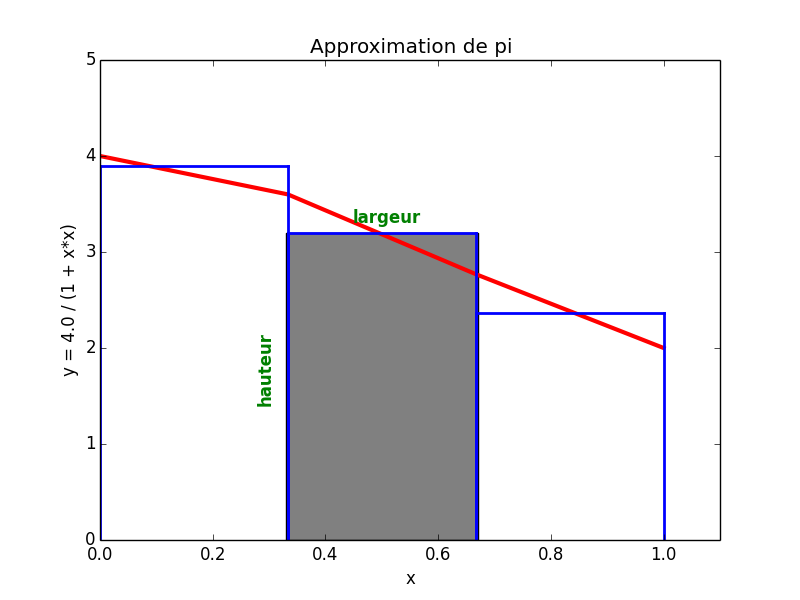
\includegraphics[height=2.2in]{images/Chapitre1/pic_pi_rect_1.png}
                \caption{\label{pic_pi_1} Approximation avec 4 rectangles}
            \end{subfigure}%
        \begin{subfigure}[t]{0.5\textwidth}
                \centering
                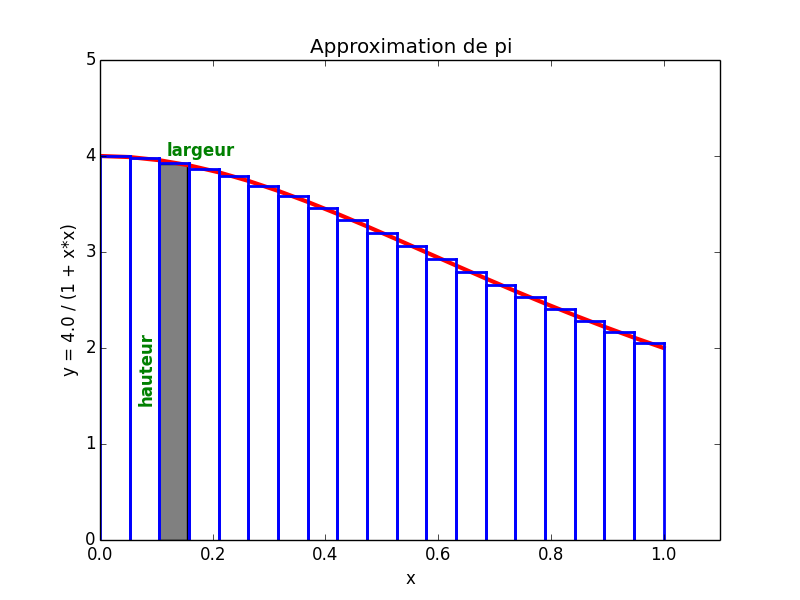
\includegraphics[height=2.2in]{images/Chapitre1/pic_pi_rect_2.png}
                \caption{\label{pic_pi_2} Approximation avec 14 rectangles}
            \end{subfigure}
            \caption{\label{pic_pi_rect} Méthode des rectangles: exemple de deux exécutions de l'algorithme avec un nombre de rectangles différents.}
            
        \end{figure}
            
        Calculer une intégrale revient à calculer l'aire formée par cette courbe et l'axe des abscisses dans le domaine étudié, ici $[0,1]$. Cette surface peut être approximée par la méthode des rectangles (ou trapèze). Cette méthode revient à dessiner des rectangles sous la courbe (voir \autoref{pic_pi_rect}). La surface de ces derniers pouvant être calculée, il est alors possible d'approcher l'intégrale donnée dans l'\autoref{eq_pi} à l'aide du code présenté dans l'extrait de code suivant:
        
        %ALGO PI
        \begin{lstlisting}[language=C, caption=Implémentation de l'algorithme de calcul d'intégrale par la méthode des rectangles, float,floatplacement=H]
double x, largeur, hauteur, pi = 0.0;

int num_steps = 4;
int num_steps = 14;

largeur = 1.0 / num_steps;

for (int i = 0; i < num_steps; ++i) {
    x =  (i) * largeur;
    hauteur = ( 4.0/(1.0+x*x));
    pi += largeur * hauteur;
}

cout << "Valeur de pi: " << pi << endl;
\end{lstlisting}
    
         Nous remarquons sur la \autoref{pic_pi_1}, qu'avec l'utilisation de quatre rectangles, la surface des rectangles ne correspond pas exactement à la courbe à approcher. Ces erreurs affectent la précision de notre programme qui affiche une valeur de $\pi = 3.38$. La \autoref{pic_pi_2} présente le même programme qui utilise 14 rectangles. Les rectangles sont alors plus fidèles à la courbe et le programme calcule une valeur de $\pi = 3.21$.
        Nous présentons cet exemple simpliste pour illustrer le besoin de puissance de calcul pour réaliser des simulations précises:
        \begin{itemize}
            \item La précision du calcul dépend du nombre de rectangles choisi. Plus le nombre de rectangles utilisés est grand, plus la précision augmente. Cependant, augmenter le nombre de rectangles à calculer augmente le nombre d'opérations nécessaires à réaliser. 
            
            \item Pour accélérer le calcul de cette application, le calcul des différents rectangles doit être réparti entre les ressources de calcul. À la fin de l'exécution, un processus s'occupe de récolter et additionner les différents résultats.
            
            \item La capacité d'une application à utiliser des ressources parallèles n'est pas automatique. Une transformation du code doit être réalisée de manière explicite (par le programmeur) ou implicite (par le compilateur).
        \end{itemize}
        
    \subsubsection{Niveau de parallélisme des supercalculateurs}
    %%%%%%%%%%%%%%%%%%%%%%%%%%%%%%%%%%%%%%%%%%%%%%%%%%%%%%%%%%%%%%
    
        La performance d'une application parallèle dépend donc du nombre et de la performance des ressources pouvant travailler simultanément pour la résolution du problème. La tâche des programmeurs est d'adapter le code pour répartir l'application sur les différentes ressources disponibles. Ce travail est difficile, car le parallélisme est présent à plusieurs niveaux dans un supercalculateur.
        
        
        \paragraph{Taxonomie de Flynn.}
             Les différentes formes de parallélisme ont été regroupées en quatre classes appelées taxonomie de Flynn \cite{Flynn2011} (voir \autoref{fig:flynn}). Ces classes permettent de caractériser les architectures en fonction de l'indépendance ou non des instructions et des données. La classe \verb=SISD= représente les architectures classiques n'exécutant qu'une instruction sur une donnée à la fois. 
            La classe \verb=SIMD= regroupe les architectures vectorielles exécutant une instruction sur plusieurs données à la fois (voir \autoref{sec:cpu_vectoriel}). La classe d'architecture \verb|MISD| exécute des instructions différentes sur le même jeu de données. Les processeurs capables d'exécuter des instructions réalisant \gls{FMA}, peuvent être considérées comme telles. Une instruction FMA permet de réaliser une addition et une multiplication sur une même donnée. Le processeur ASIC présent dans les voitures connectées peut par exemple exécuter deux algorithmes différents pour s'assurer de la validité d'une décision à prendre. La dernière classe \verb|MIMD| représente des architectures exécutant plusieurs instructions sur plusieurs données à la fois. Un serveur possédant plusieurs processeurs est un exemple d'architecture \verb|MIMD|. 
            
            \begin{figure}
            \center
            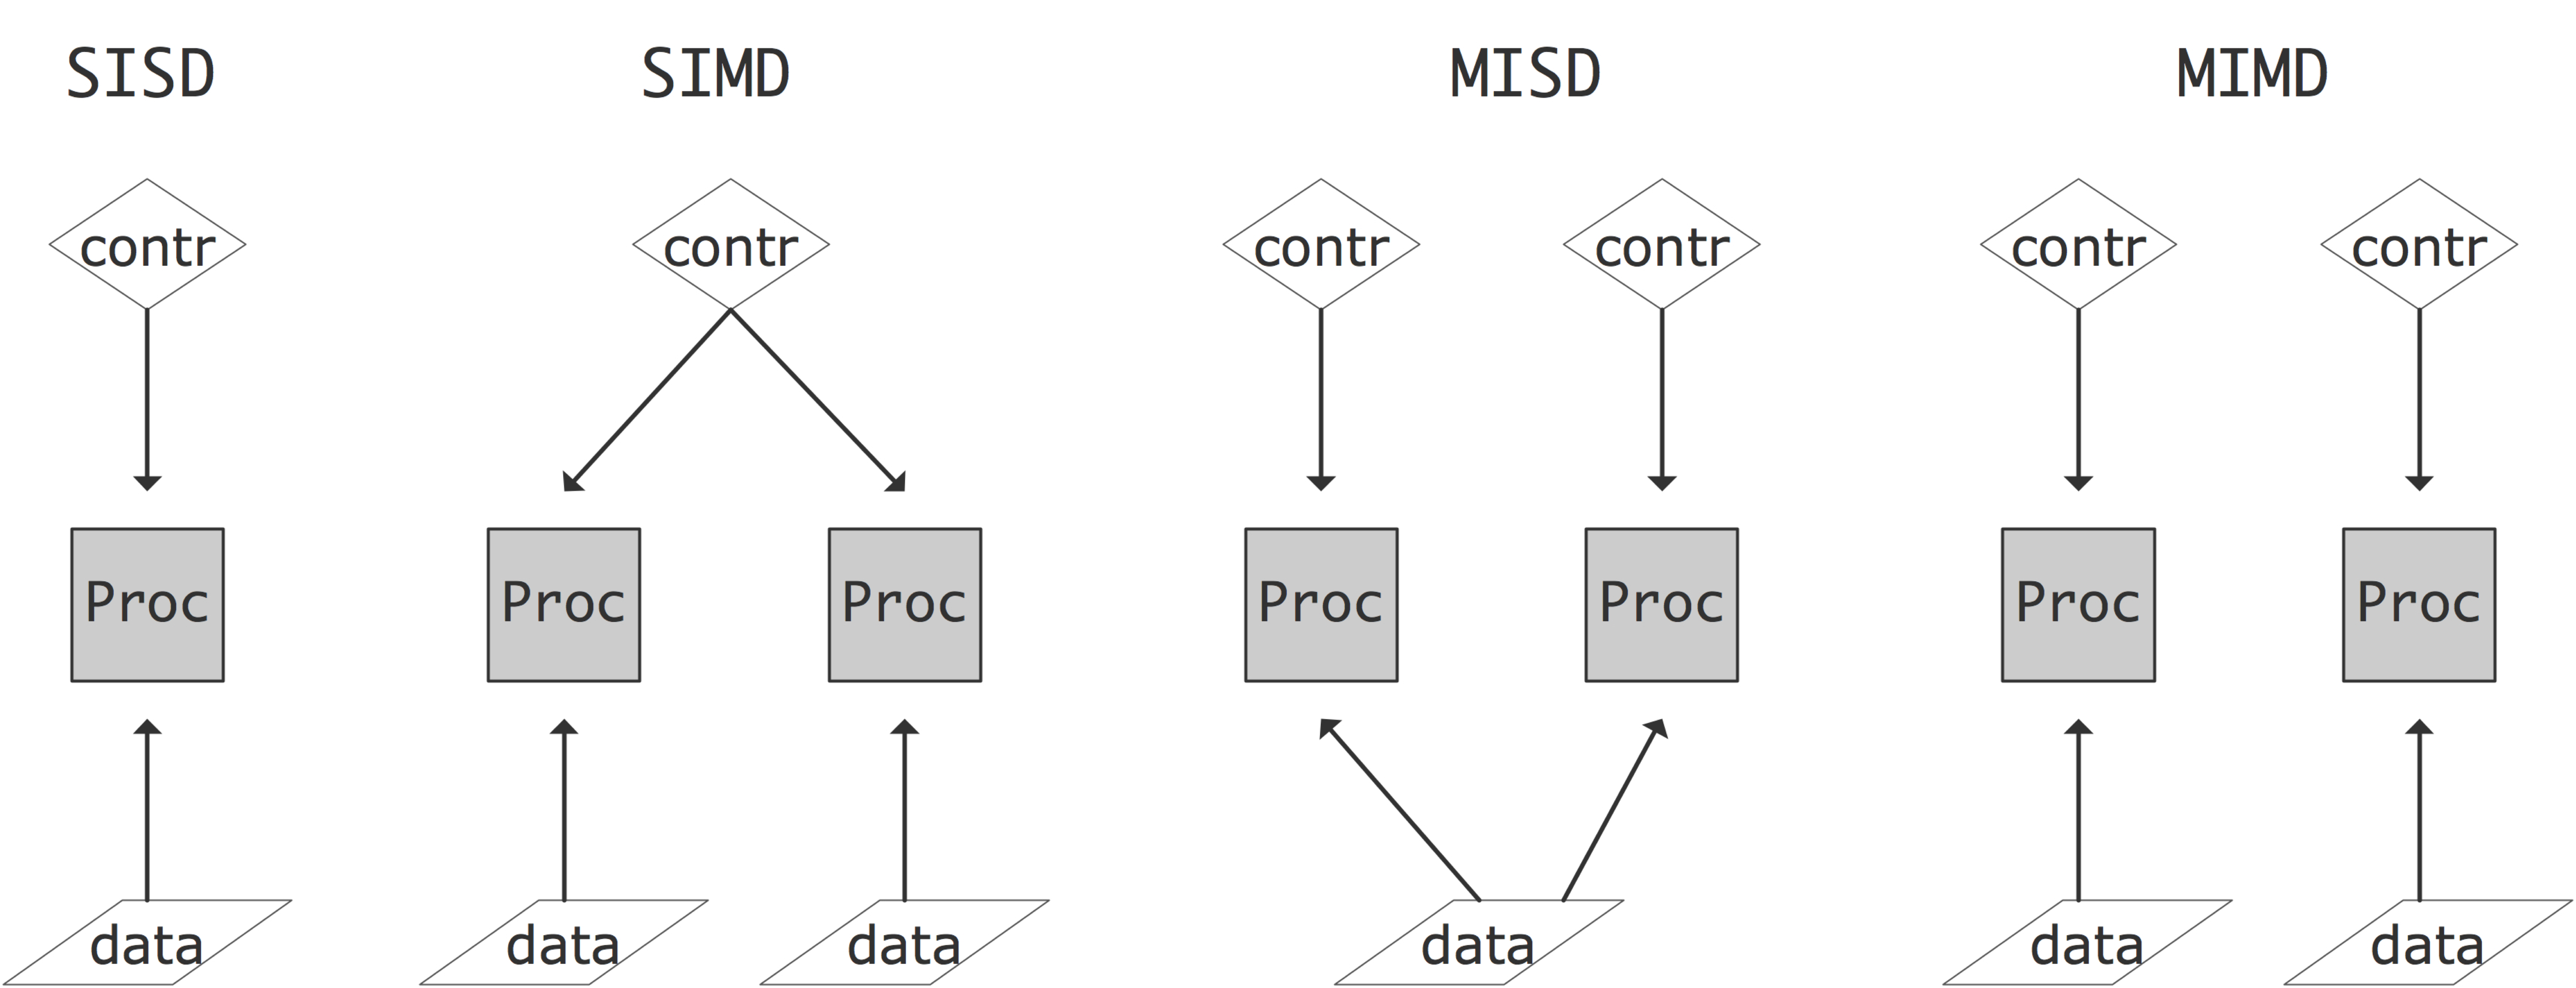
\includegraphics[width=12cm]{images/flynn.png}
            \caption{\label{fig:flynn} Les quatre classes de la taxonomie de Flynn (graphique extrait de \cite{Eijkhout2013})}
            \end{figure}
            

        \paragraph{Niveaux de parallélisme d'un supercalculateur.}
            La \autoref{fig:parallele_hpc} représente les principaux niveaux de parallélisme d'un supercalculateur. Le  niveau $1$ concerne les serveurs, reliés par un système d'interconnexion. Différentes tâches peuvent être assignées à chaque noeud qui peuvent communiquer entre eux pour se synchroniser ou partager des résultats. Le niveau $2$ concerne le parallélisme des processeurs (ainsi que des accélérateurs si le serveur en possède). En fonction des tâches à réaliser et des caractéristiques des ressources de calculs, les tâches peuvent être réparties pour être exécutées. Le niveau $3$ est situé dans les processeurs et concerne l'utilisation de processeurs multicoeurs. Le niveau $4$ est lié aux processeurs superscalaires possédant plusieurs pipelines (voir \autoref{sec:pipeline}). Le dernier niveau de parallélisme concerne les unités de calcul vectorielles des processeurs qui peuvent exécuter une instruction sur plusieurs données simultanément (voir \autoref{sec:fpu}).
            
            \begin{figure}
                \center
                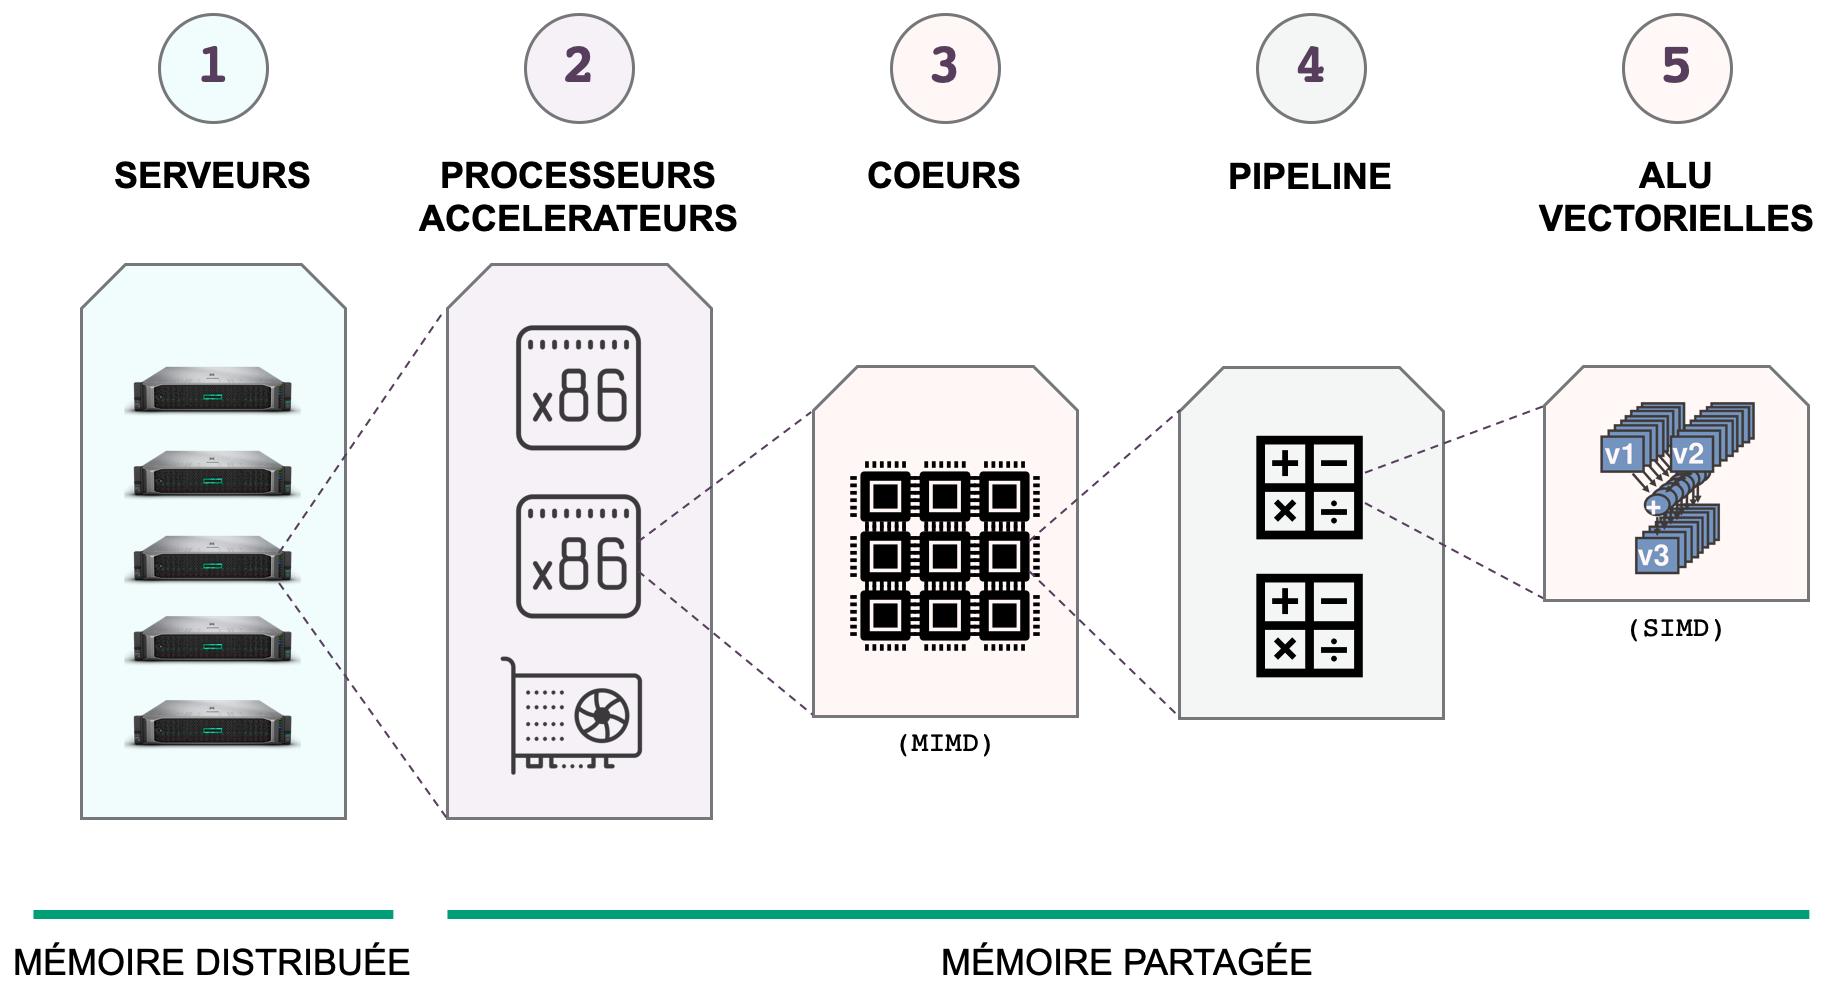
\includegraphics[width=14cm]{images/parallele_hpc.png}
                \caption{\label{fig:parallele_hpc} Différents niveaux de parallélisme dans un supercalculateur. Les processeurs MIMD sont capables d'exécuter plusieurs instructions sur plusieurs données grâce à l'utilisation de multiple coeurs. Les unités arithmétiques et logiques (ALU) peuvent exécuter une instruction sur plusieurs données à la fois (MIMD) grâce aux instructions vectorielles.}
            \end{figure}
            
            Pour maximiser le nombre d'instructions pouvant être exécutées sur un supercalculateur, (\textit{Instruction Level Parallelism} (ILP)), différentes méthodes existent. Le niveau le plus haut consiste à exécuter des applications indépendantes permettant de saturer l'utilisation de la plateforme (\textit{Job Level Parallelism}). Une même application peut être découpée en tâches qui peuvent être exécutées en parallèle (\textit{Task Level Parallelism} (TLP) \cite{Kambadur2009}). Lorsque la nature du code le permet, une instruction peut être exécutée sur plusieurs données simultanément (\textit{Data Level Parallelism}(DLP) \cite{Espasa1997}).

    \subsubsection{Paradigme de programmation}
    %%%%%%%%%%%%%%%%%%%%%%%%%%%%%%%%%%%%%%%%%%%%%%%%%%%%%%%%%%%%%%
       
        Pour pouvoir bénéficier des ressources de calculs disponibles, le programmeur doit adapter certaines parties du code. Les niveaux de parallélisme les plus bas (pipeline et ALU) sont gérés par le matériel sans intervention de l'utilisateur. Par exemple, lorsque le compilateur génère des instructions vectorielles, l'unité de calcul s'occupe seule de leur exécution. Cependant, le programmeur doit connaître les détails de la microarchitecture pour développer du code pouvant profiter du parallélisme.  Il peut par exemple adapter la structure de son code pour permettre au compilateur de présenter plusieurs instructions au module d'exécution dans le désordre (voir \aref{sec:out_of_order}) permettant ainsi d'optimiser l'utilisation des pipelines (voir \aref{sec:pipeline}) présents dans les processeurs superscalaires (voir \aref{sec:superscalar}).
        
        Pour bénéficier des niveaux $1$, $2$ et $3$ (voir \autoref{fig:parallele_hpc}), deux paradigmes fondamentaux de la programmation parallèle peuvent être utilisés: la programmation à mémoire partagée ou à mémoire distribuée. La principale distinction entre ces deux paradigmes est le partage ou non d'un espace mémoire entre les ressources utilisées (voir \autoref{fig:edl_ditribue_partage}). 
        
            \begin{figure}
                \center
                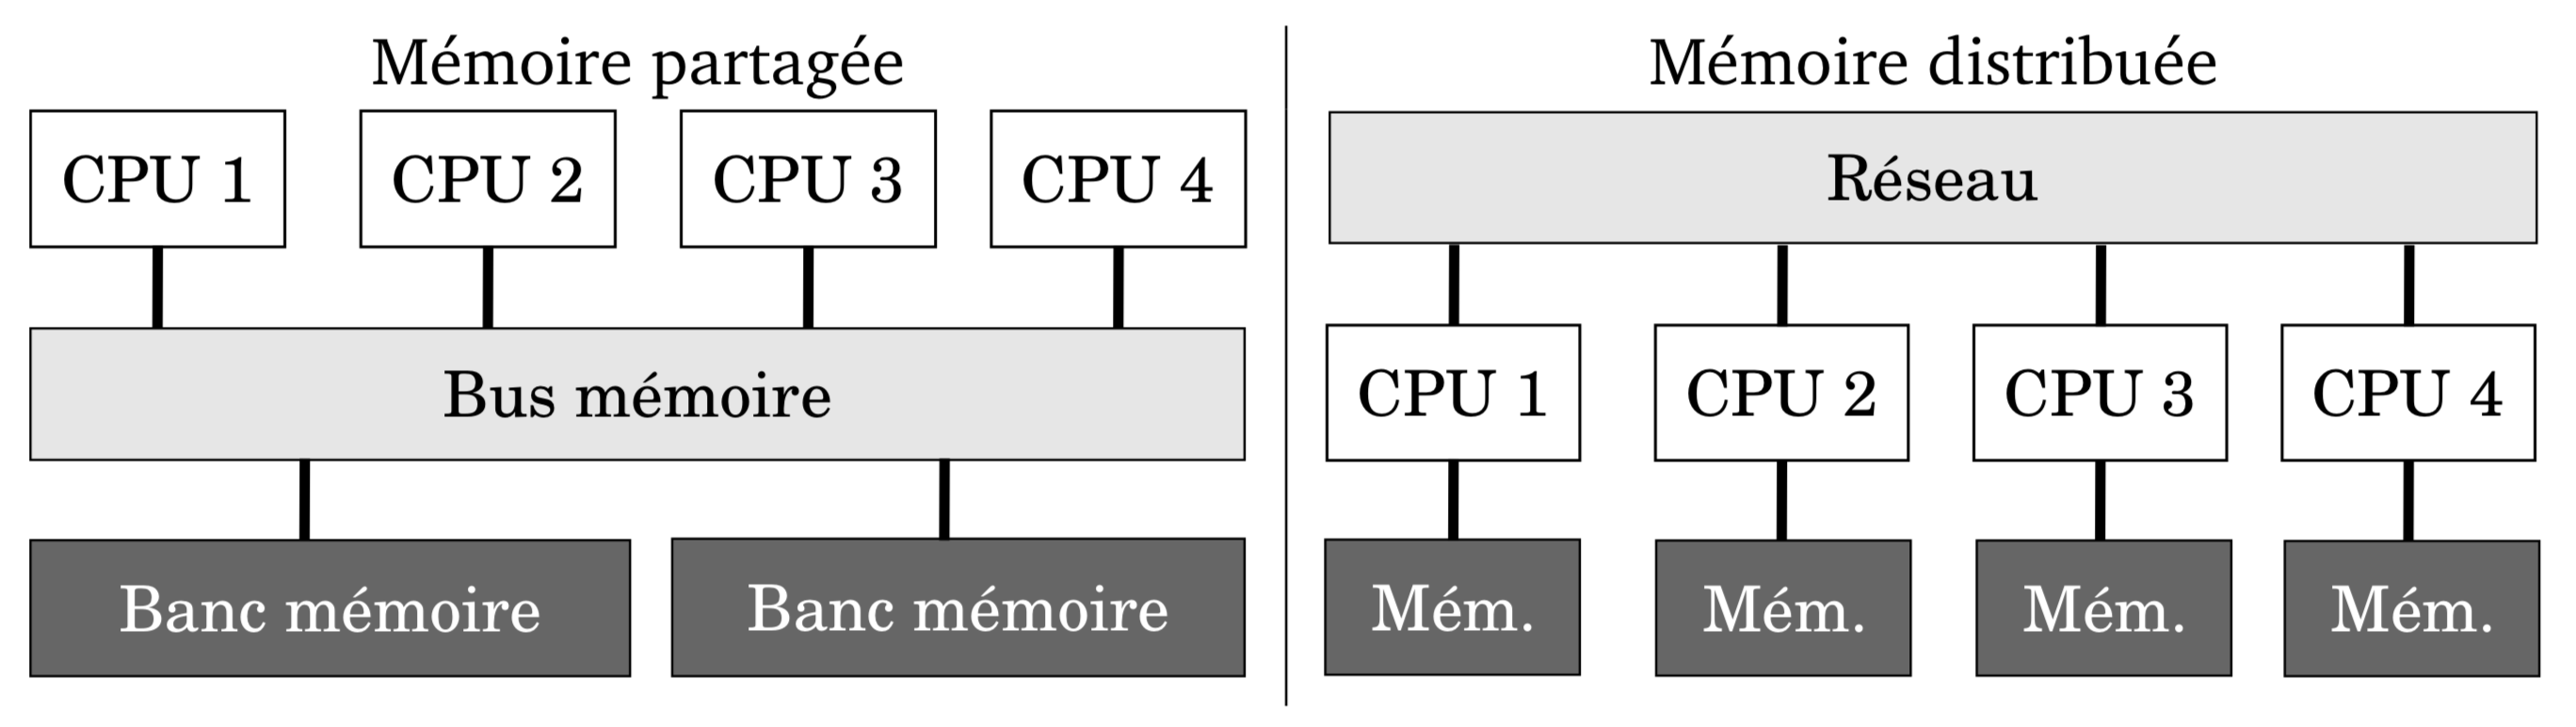
\includegraphics[width=14cm]{images/edl_ditribue_partage.png}
                \caption{\label{fig:edl_ditribue_partage} En fonction de l'architecture et du mode d'accès mémoire, deux paradigmes de programmations peuvent être utilisés (graphique extrait de \cite{Valat2016}).}
            \end{figure}
        
        
        
            
        \paragraph{Programmation à mémoire distribuée.}  
               
            Le paradigme de programmation à mémoire distribuée doit être utilisé lorsque les différents processus n'ont pas accès au même espace mémoire. Les communications entre les ressources de calculs sont alors réalisées par le système d'interconnexion. L'avantage de telles architectures est de permettre d'agréger plus ou moins de ressources en fonction du besoin d'un utilisateur. La performance de la solution est alors dépendante du nombre de serveurs utilisés et permet une plus grande flexibilité. 
            
            Les données nécessaires pour les calculs ainsi que les résultats temporaires doivent être explicitement transférés par l'utilisateur. Pour cela, les programmeurs peuvent utiliser des librairies de \textit{passage de messages}, dont le standard le plus utilisé est une \gls{mpi}. Le standard définit la sémantique des différentes fonctions, identifie les tâches distribuées et propose des moyens d'échange et de synchronisation entre les processus. Le standard est implémenté par des librairies telles que \verb|OpenMPI|, \verb|MPICH-2| ou encore \verb|IntelMPI|. Chaque noeud ayant son propre système d'exploitation, les librairies doivent être installées sur tous les serveurs utilisés. 
        
            La principale difficulté de ce paradigme de programmation est la nécessité de réaliser explicitement les mouvements de données entre les noeuds. L'exécution d'une application peut alors être résumée en 3 étapes. La \autoref{fig:scatter_gather} présente les étapes 1 et 3 d'un programme de calcul à mémoire distribuée:
            \begin{enumerate}
                \item La première étape consiste à répartir le jeu de données à l'aide d'opérations de type \textit{scatter} (voir \autoref{fig:scatter}). 
                \item La deuxième étape est la réalisation du calcul par chaque ressource. Cette étape utilise le paradigme de programmation à mémoire partagée (voir ci-dessous).
                \item Lorsque chacune d'entre elles a terminé son calcul, des opérations de type \textit{gather} (voir \autoref{fig:gather}) permettent de récolter l'ensemble des résultats partiels, pour calculer le résultat final.
            \end{enumerate}
            Les étapes 1 et 3 utilisent le système d'interconnexion du supercalculateur. La performance de celui-ci peut fortement impacter celle des applications. Cette particularité est à l'origine de nombreuses erreurs et rend la programmation à mémoire distribuée difficile. Le programmeur doit avoir à sa disposition des outils lui permettant de suivre l'évolution de chaque phase pour déceler des problèmes de synchronisation ou de déséquilibre de charge.
        
        
            \begin{figure}[t!]
                \centering
                \begin{subfigure}[t]{0.48\textwidth}
                    \centering
                    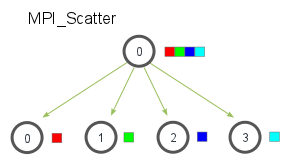
\includegraphics[width=.8\linewidth]{images/scatter.png}
                    \caption{\label{fig:scatter}Les opérations de \textit{scatter} permettent de répartir un jeu de données entre les ressources.}
                \end{subfigure}\hfill
            \begin{subfigure}[t]{0.48\textwidth}
                    \centering
                    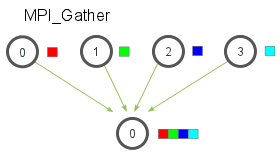
\includegraphics[width=.8\linewidth]{images/gather.png}
                    \caption{\label{fig:gather}Chaque ressource renvoie son résultat local pour calculer le résultat final du calcul.}
                \end{subfigure}
                \caption{\label{fig:scatter_gather}Les deux opérations principales de la programmation à mémoire distribuée sont de répartir (\textit{a}) et de récolter (\textit{b}) les données utilisées par les différentes ressources participant à la résolution\protect\footnotemark.}
            \end{figure}
            \footnotetext{Source des graphiques - \url{https://mpitutorial.com/tutorials/mpi-scatter-gather-and-allgather/}}
               
               
           
        %%%%%%%%%%%%%%%%%%%%%%%%%%%%%%%%%%%%%%%%%%%%%%
        \paragraph{Programmation à mémoire partagée.} \label{sec:prog_partagee}
            
            Lorsque toutes les ressources de calculs ont accès au même espace mémoire, il est conseillé d'utiliser le paradigme de programmation à mémoire partagée. Comme il n'est plus utile de transférer les données explicitement entre les ressources de calcul, il est possible d'utiliser des \gls{thread} (processus légers). Pour profiter des niveaux de parallélisme $2$ et $3$ (voir \autoref{fig:parallele_hpc}) les programmeurs peuvent avoir recours à des librairies ou même des langages spécifiques aux processeurs ciblés. Pour les processeurs, des librairies telles que \verb|OpenMP| ou \verb|Pthread| sont utilisées pour accéder au niveau $3$ de parallélisme qui consiste à répartir l'application sur les différents coeurs. Les accélérateurs de type GP-GPU peuvent être programmés à l'aide d'\verb|OpenCL| ou de \verb|CUDA|. Ces librairies sont basées sur le modèle de programmation \verb|fork/join| (voir \autoref{fig:openmp}). Lorsqu'une partie du code doit être exécutée en parallèle, le thread \textit{maître} se dédouble (\textit{fork}) en plusieurs threads pouvant être exécutés indépendamment sur différents coeurs. Une fois les tâches réalisées, les threads sont arrêtés et le programme continue son exécution séquentiellement. Ce modèle de programmation utilisant la même mémoire partagée, le programmeur doit veiller à ce que les différents threads utilisent des données en commun. Un avantage d'\verb|OpenMP| est sa facilité d'utilisation pour exprimer le parallélisme depuis le code source de l'application. À l'aide de directives préprocesseur, les zones exécutables en parallèle doivent être annotées à l'aide de \verb|#pragma|. Différentes options permettent de définir le nombre de threads à générer, la façon de partager le travail ou encore définir le mode d'accès aux données (partagé, privé). Le code listé dans l'\autoref{lst:openmp} permet de répartir les différentes itérations d'une boucle (indépendantes) entre les threads.
            
\begin{lstlisting}[language=C, caption=Distribution des itérations d'une boucle à l'aide d'OpenMP, label=lst:openmp]
#pragma omp parallel for
for (i=0;i<20;i++)
    a[i]=b[i] + 42;
\end{lstlisting}

                \begin{figure}
                \center
                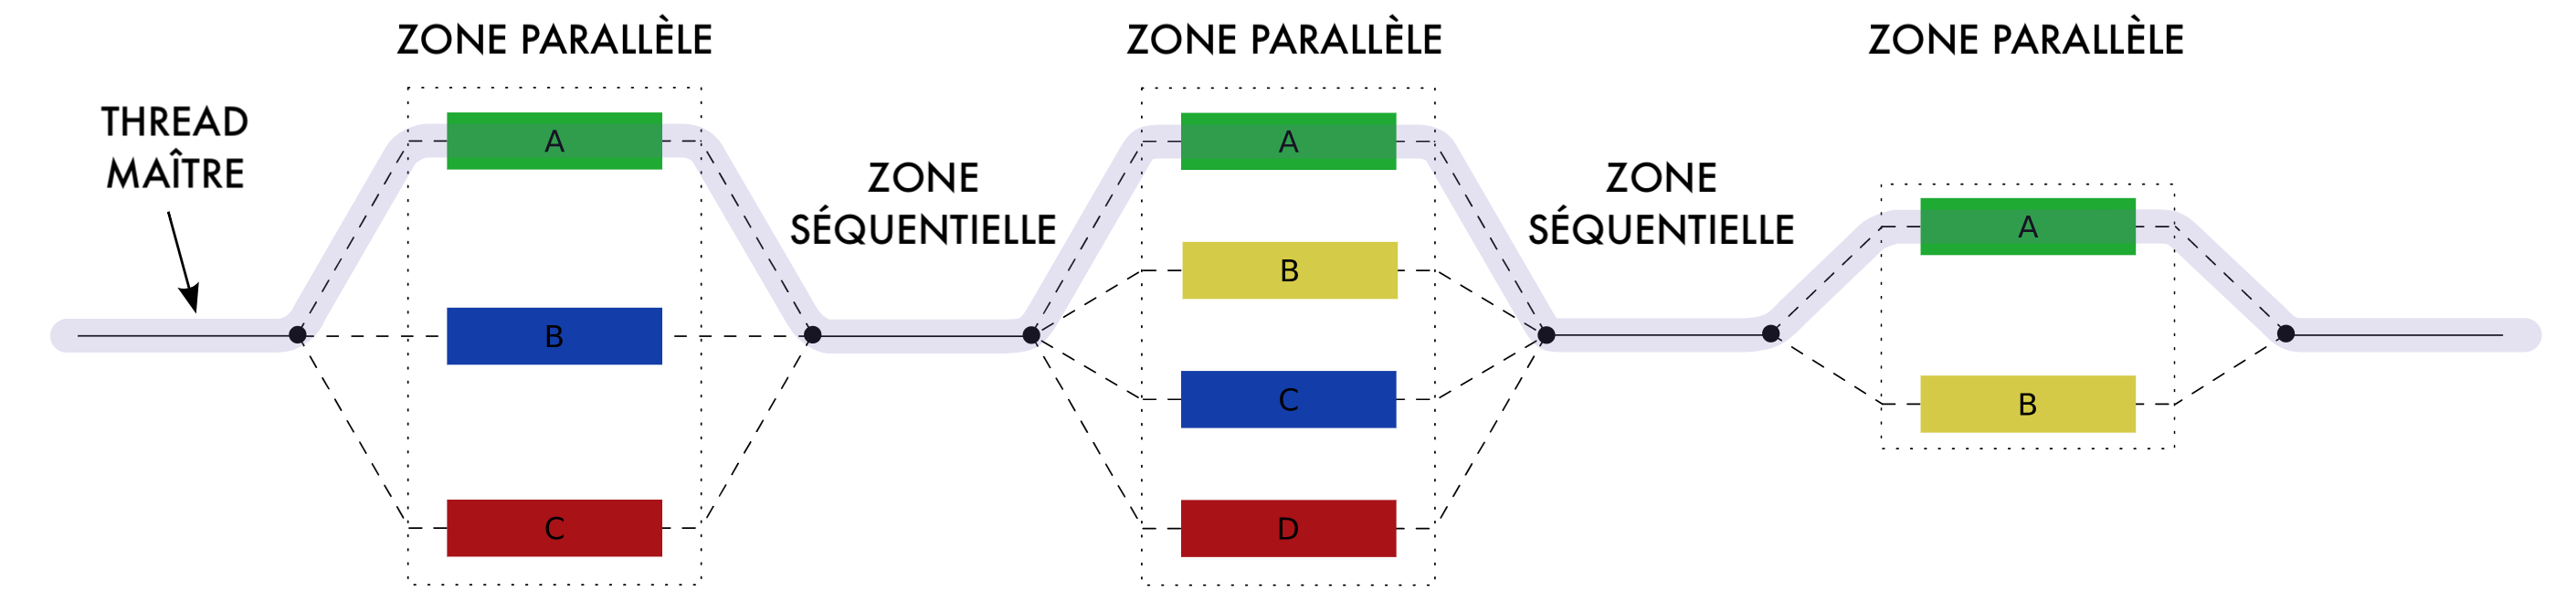
\includegraphics[width=14cm]{images/openmp.png}
                \caption{\label{fig:openmp} Pour accéder au parallélisme des coeurs, OpenMP crée des \textit{threads} indépendants\protect\footnotemark.}
                \end{figure}
                \footnotetext{Graphique adapté de \url{https://en.wikipedia.org/wiki/Fork\%E2\%80\%93join_model}}
                

\subsection{Performance de la parallélisation}
\label{sec:parallele_perf}
%%%%%%%%%%%%%%%%%%%%%%%%%%%%%%%%%%%%%%%%%%%%%%%%%%%%%%%%%%
    
        L'utilisation d'un supercalculateur a pour objectif d'accélérer l'exécution d'une application. Cette accélération peut alors permettre d'obtenir des résultats plus rapidement ou bien d'étudier des problèmes plus complexes. L'accélération d'une application, notée $Speedup(P)$, correspond au rapport entre le temps nécessaire pour exécuter l'application sur une ressource unique (noté $T_{sequentiel}$) et le temps nécessaire lorsque $P$ ressources identiques sont utilisées (noté $T_{parallele}$). L'accélération est dite optimale lorsque le temps de résolution $T_{parallele}(P)$ évolue linéairement avec le nombre $P$ de ressources. On parle alors d'accélération linéaire:
        
        \begin{equation}
        \label{eq_speedup}
        Speedup_{lineaire} (P) = \frac{T_{sequentiel}}{T_{parallele}(P)} = P
        \end{equation}
        
        Prenons l'exemple d'une application dont le temps nécessaire à l'exécution prend  $T_{sequentiel} = 2$ minutes. Une accélération linéaire avec l'utilisation de $P = 4$ processeurs pendrait alors $T_{parallele} = 30$ secondes. En pratique il est très rare d'obtenir une telle accélération, car certaines parties du code ne peuvent pas être parallélisées (transmission des données en programmation à mémoire distribuée, zone critique en programmation à mémoire partagée, synchronisation). 
        Pour évaluer la capacité d'une plateforme à utiliser efficacement les ressources supplémentaires pour l'exécution d'une application, il est courant de mesurer sa scalabilité. La scalabilité d'une application est un indicateur permettant d'évaluer sa capacité à \textit{passer à l'échelle}, c'est-à-dire d'évaluer l'accélération de son exécution lorsque des ressources de calculs supplémentaires sont allouées. On distingue alors deux scalabilités: la forte et la faible (voir \autoref{fig:scaling}). Les résultats des tests de scalabilité forte et faible permettent de choisir un nombre adapté de ressources à utiliser pour une application.
        
            \begin{figure}[t!]
                \centering
                \begin{subfigure}[t]{0.48\textwidth}
                    \centering
                    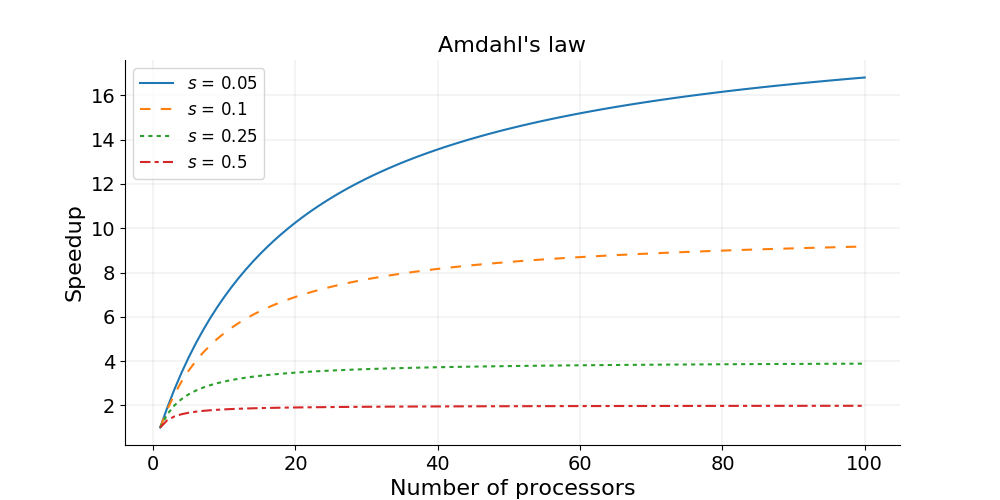
\includegraphics[width=1.05\linewidth]{images/scaling_amdahl.png}
                    \caption{\label{fig:scaling_amdahl}Loi d'Amdahl: la scalabilité forte utilise un problème de complexité constante.}
                \end{subfigure}\hfill
            \begin{subfigure}[t]{0.48\textwidth}
                    \centering
                    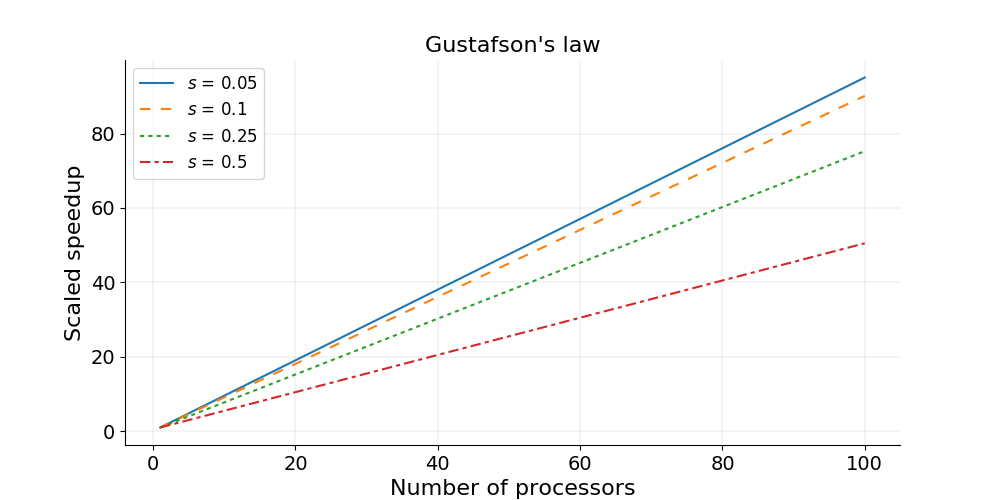
\includegraphics[width=1.05\linewidth]{images/scaling_gustafson.png}
                    \caption{\label{fig:scaling_gustafson}Loi de Gustafson: la scalabilité faible utilise un problème de complexité croissante.}
                \end{subfigure}
                \caption{\label{fig:scaling} Évolution de la scalabilité forte et faible lorsque $P$ processeurs sont utilisés pour l'exécution d'une application ayant une proportion $s$ de code séquentiel\protect\footnotemark.}
            \end{figure}
            \footnotetext{Source des graphiques - \url{https://www.kth.se/blogs/pdc/2018/11/scalability-strong-and-weak-scaling}}
            

    \subsubsection{Scalabilité forte} \label{sec:amdhal}
    %%%%%%%%%%%%%%%%%%%%%%%%%%%%%%%%%%
        
        En 1967, l'ingénieur Gene Amdahl a étudié et théorisé l'évolution de l'accélération d'une application avec l'ajout de ressources de calculs, créant ainsi la loi éponyme \cite{Amdahl1967}. La taille du problème étant fixe, chaque unité de calcul a donc moins de travail à réaliser. Idéalement, le temps d'exécution doit être réduit d'un facteur $1/P$ lorsque $P$ ressources sont ajoutées (voir \autoref{fig:scaling_amdahl}). Une application de calcul parallèle n'étant jamais totalement parallélisable, elle possède toujours une proportion de code devant être exécuté séquentiellement. Cette proportion est notée $s$. L'ajout de ressources de calcul n'est alors bénéfique que pour la proportion de code dit parallélisable et noté $1-s$. Le temps nécessaire pour l'exécution de l'application est la somme du temps passé dans la zone séquentielle et de celui passé dans la zone parallèle. En utilisant $P$ processeurs le temps de l'exécution parallèle peut être calculé ainsi: 

        
            \begin{equation}
            T_{parallele}(P) = s \times T_{sequentiel} + \frac{(1-s) \times T_{sequentiel}}{P}
            \end{equation}
        
        L'accélération de l'application peut alors être calculée grâce à l'\autoref{eq_speedup} donnant lieu à l'équation suivante, appelée loi d'Amdahl:
        
                
            \begin{equation}
            \label{eq_amdahl}
            Speedup (P) = \frac{T_{sequentiel}}{s \times T_{sequentiel} + \frac{(1-s) \times T_{sequentiel}}{P}} =  \frac{1}{s + \frac{1-s}{P}}
            \end{equation}
        
        L'accélération d'une application dépend donc du nombre de ressources de calculs supplémentaires allouées à la résolution de l'application, mais aussi de la proportion de zones exécutables en parallèle. La \autoref{fig:scaling_amdahl} montre l'importance de l'influence de la proportion de code séquentiel $s$ sur l'accélération de l'application. Grâce à la loi d'Amdahl, il est possible de donner la limite théorique de l'accélération $Speedup$ d'une application (notée $Speedup_{max}$),  lorsque des ressources de calculs supplémentaires sont utilisées pour la résolution d'un problème de taille fixe. L'accélération maximale d'une application utilisant 95\% de son temps d'exécution dans une fonction entièrement parallélisable peut être calculée par la limite suivante:         
        \begin{equation}
        Speedup_{max} =  \lim_{p\to\infty}    \frac{1}{0.05 + \frac{0.95}{P}} = \frac{1}{0.05} = 20         
        \end{equation}
        Quel que soit le nombre de ressources allouées à l'exécution de cette application, l'application étudiée en exemple ne pourra jamais être accélérée de plus de 20 fois.  
        
        
        %Les coûts engendrés par ces différentes opérations sont notés $T_{couts}$. La durée de l'exécution du programme parallèle peut alors être calculée par la formule suivante:
                %En supposant des coûts $T_{couts}$ associés à l'utilisation du parallélisme, le temps d'exécution du programme parallélisé peut être calculé ainsi:
        %\begin{equation}
        %T_{parallele} = \frac{T_{sequentiel}}{P} + T_{couts}
        %\end{equation}
        
       
    \subsubsection{Scalabilité faible} 
    %%%%%%%%%%%%%%%%%%%%%%%%%%%%%%%%%%
        
        La loi d'Amdahl est très utile pour montrer la nécessité de développer des applications avec la plus grande portion de code parallélisable. Cependant, la loi suppose une taille de problème constante. Lorsque des ressources de calculs supplémentaires sont disponibles, les applications utilisent généralement des jeux de données plus grands pour profiter de l'espace mémoire supplémentaire. La loi d'Amdahl supposant un jeu de donnée fixe n'est alors pas adaptée. Pour y remédier, Gustafson énonça une nouvelle loi en 1988 \cite{Gustafson1988} permettant de prendre cet aspect en considération. 
        Lorsque la taille du jeu de données augmente, la partie séquentielle du programme représente généralement une plus faible portion, car les données sont traitées dans les zones parallèles. Pour une application ayant une proportion de $1-s$ pouvant être exécutée en parallèle sur $P$ processeur, l'accélération peut être calculée par la loi de Gustafson:         
        \begin{equation}
            Speedup (P) = s + (1-s) * P         
        \end{equation}
        
        La scalabilité faible utilise une taille de problème qui évolue à mesure que des ressources supplémentaires sont allouées. Dans ce cas-là, la taille du problème pour chaque unité de calcul est fixe. Dans l'idéal, le temps d'exécution de l'application doit rester constant lors de l'ajout de ressources de calculs (voir \autoref{fig:scaling_gustafson}). Contrairement à la scalabilité forte, l'accélération obtenue par la scalabilité forte n'a pas de limite théorique. 
        
        
\section{Évolution de la performance des supercalculateurs}\label{sec:edl_evolution}
%%%%%%%%%%%%%%%%%%%%%%%%%%%%%%%%%%%%%%%%%%%%%%%%%%%%%%%%%%%

La performance des supercalculateurs a beaucoup évolué depuis leur apparition. Pour comprendre les défis que l'industrie doit relever pour poursuivre ces améliorations, nous nous sommes intéressés à l'évolution des performances de ces architectures ces 20 dernières années.


\subsection{Comparer la performance des supercalculateurs}
%%%%%%%%%%%%%%%%%%%%%%%%%%%%%%%%%%%%%%%%%%%%%

    Pour mesurer et comparer la performance des supercalculateurs, il est nécessaire d'avoir une application de référence. L'étalonnage (\textit{benchmarking}) est une pratique courante qui consiste à évaluer plusieurs solutions en leur faisant passer une épreuve commune. Dans le domaine informatique, cela permet de tester différentes architectures matérielles et d'évaluer leurs performances. Un des benchmarks les plus utilisés dans le domaine du HPC est celui développé par Jack Dongara en 1988: le benchmark HPL (High-Performance Linpack) \cite{Dongarra2003}. Ce benchmark est un code simple qui résout un système d'équations linéaires $Ax = B$, $A$ et $B$ étant deux matrices. Les performances évoluent linéairement avec le nombre de machines utilisées, car très peu de communications sont nécessaires. Le résultat est un nombre d'\gls{FLOPS} que la machine peut exécuter, ce qui rend la comparaison entre supercalculateurs aisée.
    Ce code permet de publier deux classements bisannuels: le Top500 et le Green500 (\autoref{fig:Top500}).

        \begin{figure}[b!]
                \centering
                \begin{subfigure}[t]{0.48\textwidth}
                    \centering
                    
\includegraphics[width=.4\linewidth]{images/Top500_logo.png}
                    \caption{\label{fig:Top500_logo}Top500}
                \end{subfigure}\hfill
            \begin{subfigure}[t]{0.48\textwidth}
                    \centering
                    
\includegraphics[width=.25\linewidth]{images/Green500_logo.png}
                    \caption{\label{fig:Green500_logo}Green500}
            \end{subfigure}
            \caption{\label{fig:Top500} Les classements du Top500 et du Green500 sont présentés deux fois par an lors de la conférence Supercomputing\protect\footnotemark}
        \end{figure}
        \footnotetext{\url{supercomputing.org/}}
        
    \subsubsection{Le Top500}\label{sec:Top500}
    %%%%%%%%%%%%%%%%%%%%%%%%%%%%%%%%%%%%%%%%%%%%%
        
        Le TOP500\footnote{\url{www.top500.org}} est un classement mondial qui classe, tous les 6 mois depuis 1993, les 500 supercalculateurs les plus puissants au monde. Ce classement se base sur le nombre maximum d'opérations flottantes qui peuvent être exécutées en une seconde (\gls{FLOPS}) lors de l'exécution du benchmark HPL. Cette unité a été choisie, car la grande majorité des codes utilisés dans les domaines précédemment cités exécutent des opérations sur des nombres flottants. Il s'avère donc judicieux de choisir ce dénominateur commun pour comparer les différentes architectures.

        Il faut cependant savoir que ce classement ne contient pas toutes les machines. En effet, certains industriels ne préfèrent pas apparaître dans ce classement. Stratégiquement parlant, il peut être intéressant de ne pas publier sa puissance de calcul et nous savons que certaines des infrastructures les plus puissantes n'y figurent pas. Cependant, ce classement permet d'apprécier les tendances que suivent la majorité des architectures.
        
        Au moment de l'écriture de ce manuscrit, le dernier classement disponible est celui de novembre 2019\footnote{Top500 novembre 2019 -  \url{www.top500.org/lists/2019/11/}}. Les principales caractéristiques des quatre premiers supercalculateurs sont présentées dans le \autoref{tab:top500}. Les États-Unis et la Chine possèdent chacun deux entrées et se partagent 70\% des performances totales du Top500 (32.3\% pour la Chine, 37.1\% pour les États-Unis). Concernant le système d'interconnexion, 6 des 10 premières entrées, ainsi que 141 des 500 supercalculateurs,  utilisent la technologie Infiniband.
        L'efficacité des supercalculateurs représente la capacité d'une plateforme à atteindre la performance théorique \verb|Rpeak|. Sur les 500 plateformes répertoriées, 100 d'entre elles ne parviennent pas à atteindre plus de 50\% de la performance théorique. Cette information est importante pour comprendre la difficulté qu'ont les applications à utiliser ces plateformes efficacement. Le benchmark \verb|HPL| est un code très simple, avec peu d'accès mémoire. Les applications réelles, plus complexes, ont beaucoup de mal à atteindre la performance théorique. Depuis quelques années, le classement du Top500 donne la performance d'un second benchmark (HPCG, voir \autoref{sec:hpcg}). Pour ce benchmark, plus fidèle aux comportements d'applications réelles, aucune des plateformes n'atteint une efficacité supérieure à 4\%. Pour avoir une meilleure vision de l'efficacité des plateformes, le classement du Green500 peut être consulté.


        \begin{table}[]
\centering
\resizebox{\textwidth}{!}{%
\begin{tabular}{|c|c|c|r|r|r|c|r|r|r|}
\hline
\rowcolor[HTML]{EFEFEF} 
\textbf{Pos.} & \textbf{Nom} & \multicolumn{1}{l|}{\cellcolor[HTML]{EFEFEF}\textbf{Country}} & \multicolumn{1}{l|}{\cellcolor[HTML]{EFEFEF}\textbf{Nb. coeurs}} & \multicolumn{1}{l|}{\cellcolor[HTML]{EFEFEF}\textbf{Coeurs accélérateur}} & \multicolumn{1}{l|}{\cellcolor[HTML]{EFEFEF}\textbf{Alimentation (MW)}} & \multicolumn{1}{l|}{\cellcolor[HTML]{EFEFEF}\textbf{Accélérateur}} & \multicolumn{1}{c|}{\cellcolor[HTML]{EFEFEF}\textbf{Rpeak}} & \multicolumn{1}{c|}{\cellcolor[HTML]{EFEFEF}\textbf{Rmax}} & \multicolumn{1}{c|}{\cellcolor[HTML]{EFEFEF}\textbf{Éfficacité}} \\ \hline
1 & Summit & United States & 2414592 & 2211840 & 10 & NVIDIA GPU & 200 & 148 & 0.74 \\ \hline
2 & Sierra & United States & 1572480 & 1382400 & 7 & NVIDIA GPU & 125 & 94 & 0.75 \\ \hline
3 & Sunway TaihuLight & China & 10649600 & 0 & 15 & None & 125 & 93 & 0.74 \\ \hline
4 & Tianhe-2A & China & 4981760 & 4554752 & 18 & Matrix-2000 & 100 & 61 & 0.61 \\ \hline
\end{tabular}%
}
\caption{Classement du Top500 de novembre 2019. Les puissances Rpeak (puissance théorique) et Rmax (puissance mesurée par HPL) sont données en pétaFLOPS ($10^{15}$ FLOPS). L'efficacité est le rapport entre Rmax et Rpeak.}
\label{tab:top500}
\end{table}
   
    \subsubsection{Le Green500}
    %%%%%%%%%%%%%%%%%%%%%%%%%%%%%
        
        Un second classement a vu le jour en 2007 appelé le Green500\footnote{Green500 - \url{www.top500.org/green500/}}. Il classe les supercalculateurs selon un critère d'efficacité énergétique. Cette efficacité mesure le nombre d'opérations sur un nombre flottant réalisé pour 1 watt d'énergie fourni au supercalculateur. 
    
        En effet, ces vingt dernières années, les évolutions technologiques et l'augmentation de la taille des supercalculateurs n'avaient pas de limite physique. Cette course à la performance n'était dictée que par les budgets disponibles pour leur construction. Ainsi, l'émergence de plateformes consommant de grandes quantités d'énergie et très peu efficace a été constatée (voir le classement du Top500). 
        
        En novembre 2019\footnote{\url{www.top500.org/green500/lists/2019/11/}}, les 34 premiers supercalculateurs utilisent tous des accélérateurs. La majorité étant des GPU Nvidia Tesla. Il est intéressant de noter que la deuxième place du classement est tenue par une plateforme basée sur le processeur PEZY-SC2 conçu par l'entreprise PEZY et fabriqué par TSMC. Seul le premier du classement n'utilise pas d'accélérateurs (voir \autoref{tab:green500}). Il utilise un processeur ARM basse fréquence pouvant exécuter des instructions vectorielles SVE (Scalable Vector Extensions) sur 512 bits.

        
        \begin{table}[]
            \centering
            \resizebox{0.80\textwidth}{!}{%
            \begin{tabular}{|c|r|l|l|r|r|r|r|}
            \hline
            \rowcolor[HTML]{EFEFEF} 
            \textbf{Position} & \multicolumn{1}{c|}{\cellcolor[HTML]{EFEFEF}\textbf{TOP500}} & \multicolumn{1}{c|}{\cellcolor[HTML]{EFEFEF}\textbf{Processeur}} & \multicolumn{1}{c|}{\cellcolor[HTML]{EFEFEF}\textbf{Accélérateur}} & \multicolumn{1}{c|}{\cellcolor[HTML]{EFEFEF}\textbf{Rmax}} & \multicolumn{1}{c|}{\cellcolor[HTML]{EFEFEF}\textbf{Rpeak}} & \multicolumn{1}{c|}{\cellcolor[HTML]{EFEFEF}\textbf{Efficacité}} & \multicolumn{1}{c|}{\cellcolor[HTML]{EFEFEF}\textbf{Efficacité énergétique}} \\ \hline
            1 & 159 & Fujitsu A64FX & Aucun & 1.99 & 2.35 & 0.84 & 16.876 \\ \hline
            2 & 420 & Xeon D-1571 & PEZY-SC2 700Mhz & 1.30 & 1.79 & 0.72 & 16.256 \\ \hline
            3 & 24 & IBM POWER9 & Volta GV100 & 8.04 & 11.12 & 0.72 & 15.771 \\ \hline
            4 & 373 & IBM POWER9 & Tesla V100 SXM2 & 1.46 & 1.73 & 0.84 & 15.574 \\ \hline
            \end{tabular}%
            }
            \caption{Classement du Green500 de novembre 2019 selon l'efficacité énergétique (en gigaFLOPS/Watts). Les puissances Rpeak (puissance théorique) et Rmax (puissance mesurée par HPL) sont données en pétaFLOPS ($10^{15}$ FLOPS).}
            \label{tab:green500}
        \end{table}
        
        
\subsection{Évolution des performances des supercalculateurs}
%%%%%%%%%%%%%%%%%%%%%%%%%%%%%%%%%%%%%%

    Le classement du Top500 a de nombreux avantages, dont celui de promouvoir le HPC au grand public. Cependant, un effet de bord de ce classement est de motiver les constructeurs pour développer des architectures ayant de bonnes performances lors de l'exécution du benchmark HPL. Or, ce code n'est pas représentatif des applications réelles et nous pouvons nous demander si son utilisation pour l'établissement du Top500 n'a pas été contre-productive. Bien que certains des supercalculateurs les plus puissants n'y figurent pas, l'évolution du Top500 permet d'obtenir un aperçu des évolutions de performances des architectures.
    
    Pour avoir une vision globale de son évolution, nous étudions la performance cumulée des 500 supercalculateurs depuis le premier classement (voir \autoref{pic_top500perf_evo}). Nous distinguons deux phases: avant et après 2012. 
    Les performances du Top500 ont évolué d'un facteur 1000 tous les 11 ans, conformément aux performances prédites par la loi de Moore. À partir de 2013, il faut attendre en moyenne 20 ans pour voir la performance des supercalculateurs augmenter dans la même proportion.
    Dans cette section, nous discutons des différents facteurs qui ont permis l'évolution constante des performances des architectures pendant près de 20 ans et étudions les freins qui empêchent de poursuivre ce rythme. La majorité des améliorations évoquées sont présentées dans l'\aref{chap:sota:materiel}.

    
    \begin{figure}
        \center
        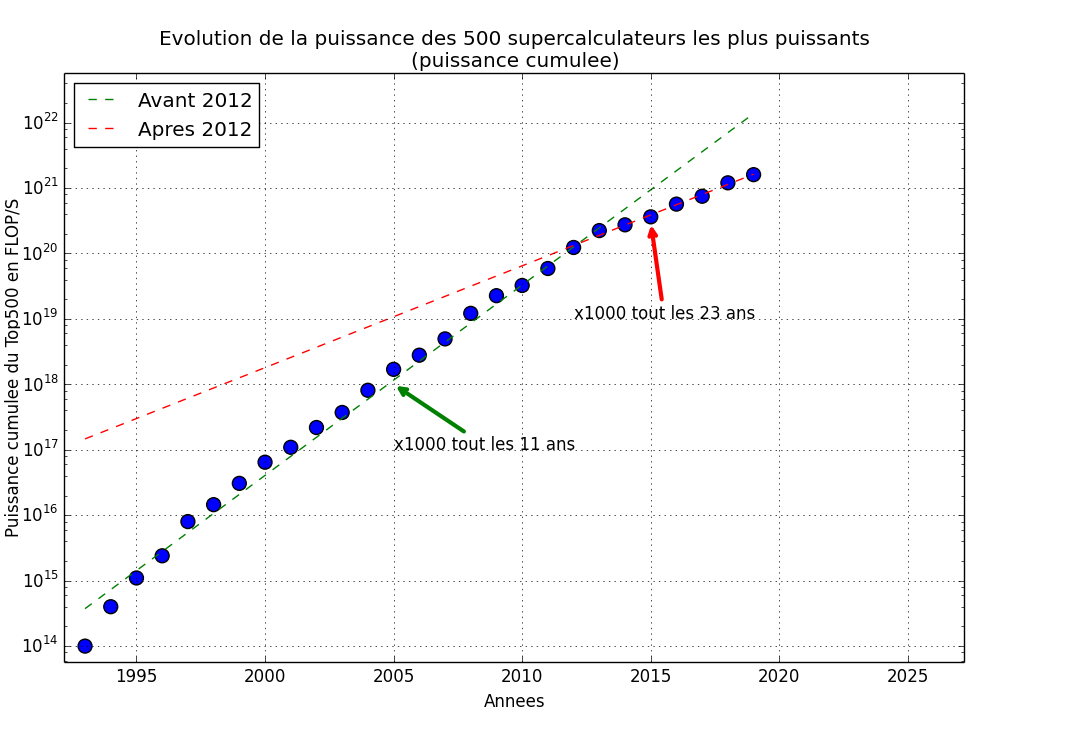
\includegraphics[width=12cm]{images/top500_evolution.png}
        \caption{\label{pic_top500perf_evo} Évolution de la performance cumulée des 500 supercalculateurs les plus puissants au monde. La pente de l'évolution diminue à partir de 2012.}
    \end{figure}


    \subsubsection{Avant 2012}\label{sec:proc_evo_2012}
    %%%%%%%%%%%%%%%%%%%%%%%%%%%%
    
        Les supercalculateurs ont pu bénéficier de nouvelles technologiques ainsi que de nombreuses innovations techniques.
        
        \begin{figure}[t!]
            \centering
            \begin{subfigure}[t]{0.33\textwidth}
                \centering
                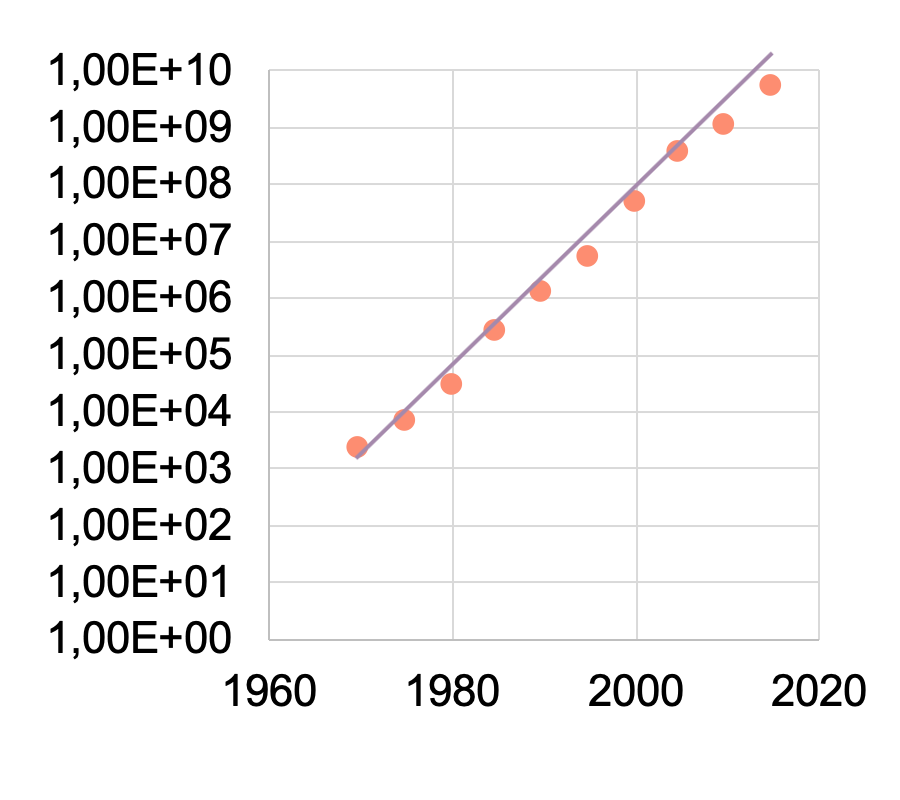
\includegraphics[width=\linewidth]{images/evo_transistor.png}
                \caption{\label{fig:evo_transistor}Évolution du nombre de transistors (\autoref{sec:denard})}
            \end{subfigure}\hfill
            \begin{subfigure}[t]{0.33\textwidth}
                \centering
                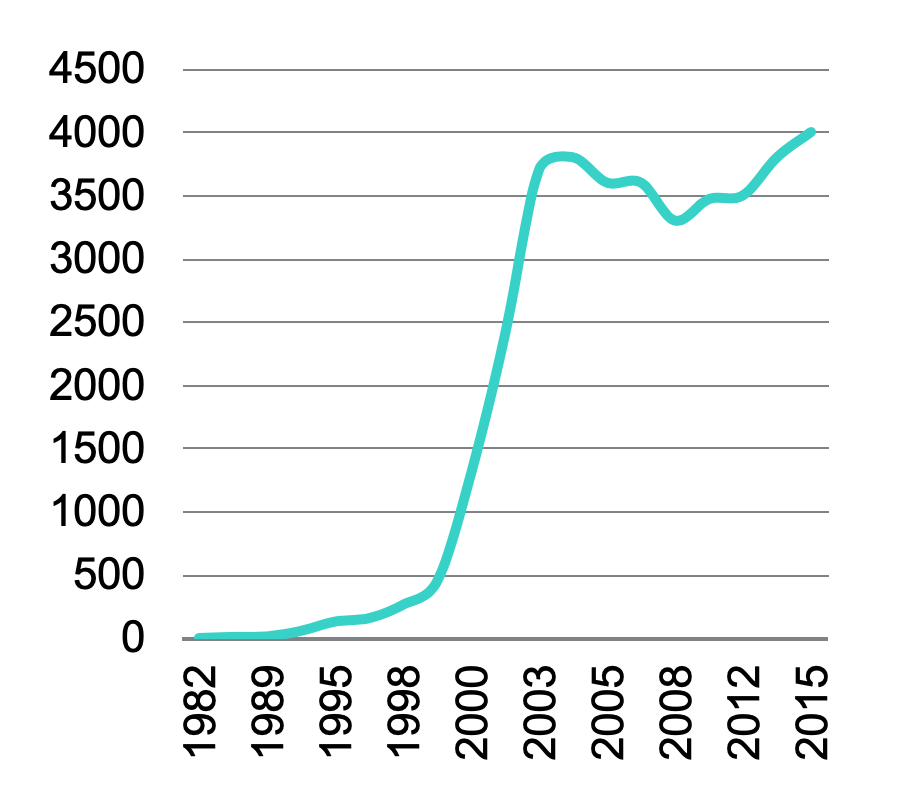
\includegraphics[width=\linewidth]{images/evo_freq.png}
                \caption{\label{fig:evo_freq}Évolution de la fréquence (\autoref{sec:frequency})}
            \end{subfigure}\hfill
            \begin{subfigure}[t]{0.33\textwidth}
                    \centering
                    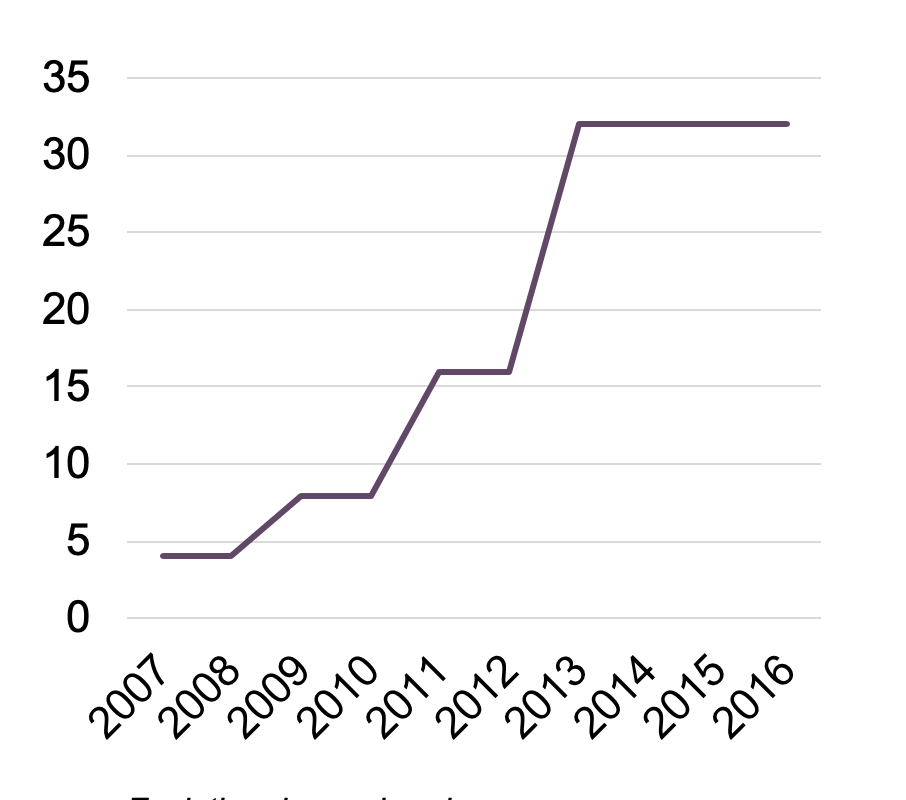
\includegraphics[width=\linewidth]{images/evo_core.png}
                    \caption{\label{fig:evo_core}Évolution du nombre de coeurs (\autoref{sec:multicore})}
            \end{subfigure}
            \caption{\label{fig:evo_proc}Évolutions technologiques principales des processeurs. Ces différentes évolutions sont présentées dans l'\autoref{annexe:CHAPITRE_ARCHITECTURE}.}
        \end{figure}
        
            \paragraph{Les processeurs.} Dans l'\aref{chap:sota:materiel}, nous présentons les différentes évolutions technologiques dont ont pu bénéficier les processeurs. La \autoref{fig:evo_proc} résume les trois principales évolutions.
            Grâce à l'affinement des procédés de gravure, le nombre de transistors a évolué exponentiellement (voir \autoref{fig:evo_transistor}).  
            En miniaturisant les transistors et en utilisant des systèmes de refroidissement plus efficaces, la fréquence des processeurs a pu être augmentée de plusieurs facteurs (voir \autoref{fig:evo_freq}).
            Lorsque la fréquence n'a plus pu être augmentée, les architectures parallèles ont été développées, donnant naissance aux processeurs multicoeurs (voir \autoref{fig:evo_core}). La microarchitecture elle-même a reçu de nombreuses améliorations: l'utilisation de pipeline (voir \autoref{sec:pipeline}) pouvant être superscalaire (voir \autoref{sec:superscalar}), ainsi que le développement d'unités de calculs pouvant exécuter des instructions vectorielles (voir \autoref{sec:cpu_vectoriel}).
            
            \paragraph{Les mémoires.} La performance des processeurs évoluant, celle des mémoires a aussi dû être amélioré pour fournir les données nécessaires aux traitements plus rapidement. Les principales améliorations sont dues à l'utilisation de nouvelles technologies mémoires (voir \autoref{sec:memory}), l'augmentation du nombre de canaux reliant la mémoire au processeur ou encore l'implémentation d'une hiérarchie de mémoire (voir \autoref{sec:hierarchie_true}). Celle-ci permettant aux applications de profiter du principe de localité (voir \autoref{sec:locality}).
            
        
    \subsubsection{Après 2012}
    %%%%%%%%%%%%%%%%%%%%%%%%%%%%
    
        En étudiant l'évolution de la puissance des supercalculateurs (voir \autoref{pic_top500perf_evo}), nous remarquons un ralentissement à partir des années 2010-2012. Ce ralentissement n'est pas dû à un seul facteur, mais à un ensemble de contraintes. En effet, les leviers et évolutions technologiques qui permettaient de tenir cette cadence ne sont plus disponibles aujourd'hui ou sont en fin de course (voir \autoref{fig:evo_proc}). Si certaines lois ont assuré une évolution continue de la performance des processeurs pendant plusieurs dizaines d'années, une partie du ralentissement de l'évolution des performances du Top500 peut être expliquée par leur \textit{essoufflement} \cite{FrancoisBodin2015}.

       
        \begin{figure}
            \center
            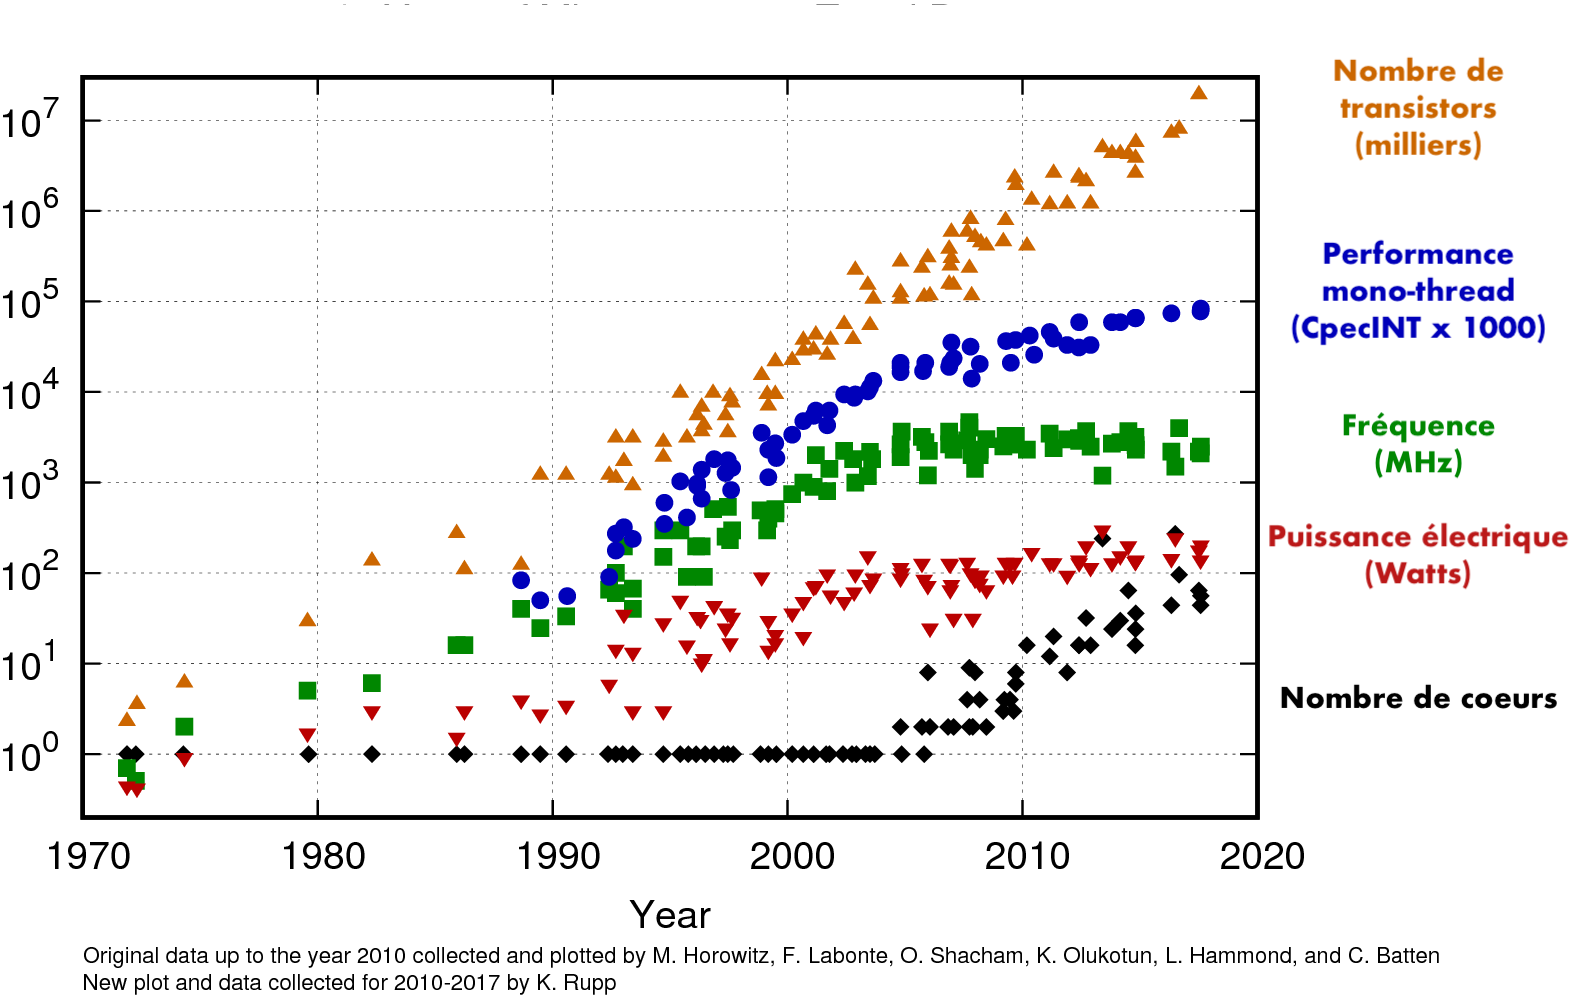
\includegraphics[width=12cm]{images/evo_proc.png}
            \caption{\label{fig:evo_proc} Évolution des principales caractéristiques des processeurs (données originales tirées de \cite{rupp40years}\protect\footnotemark).}
        \end{figure}
        \footnotetext{Les données sont accessibles sur le dépôt GitHub de l'auteur:  \url{https://github.com/karlrupp/microprocessor-trend-data}}
        
%%%%%%%%%%%%%%%%%%%%%%%%%%%%%%%%%%%%%%%%%%%%%%%%%%%%%%%%%%%%%%%%%%%%%%%%%%%% 
      
        \paragraph{Fin de validité de la loi de Moore.}\label{sec:end_mooore} 
            
            La loi de Moore \cite{Moore1998} prévoyait que les architectures pourraient doubler leur nombre de transistors, tous les deux ans \cite{Moore75}, à coût constant (voir \autoref{sec:moore}). Malheureusement, les fondeurs ne parviennent plus à suivre le rythme dicté par la loi énoncée par Gordon Moore, pour des raisons principalement techniques (gravure), de coût \cite{Brooks2017} et de limite physique. La miniaturisation continue des transistors, dont la taille actuelle est de quelques nanomètres, rend la circulation des courants électriques instable. La bonne circulation des signaux électriques dans les circuits ne pouvant plus être garantie, il n'est alors plus possible de réduire leur taille.
            À partir de 2013, l'évolution des performances du Top500 passe pour la première fois sous les performances prévues par la loi de Moore (\autoref{fig:moore_vs_top500}).
            

            \begin{figure}
            \center
            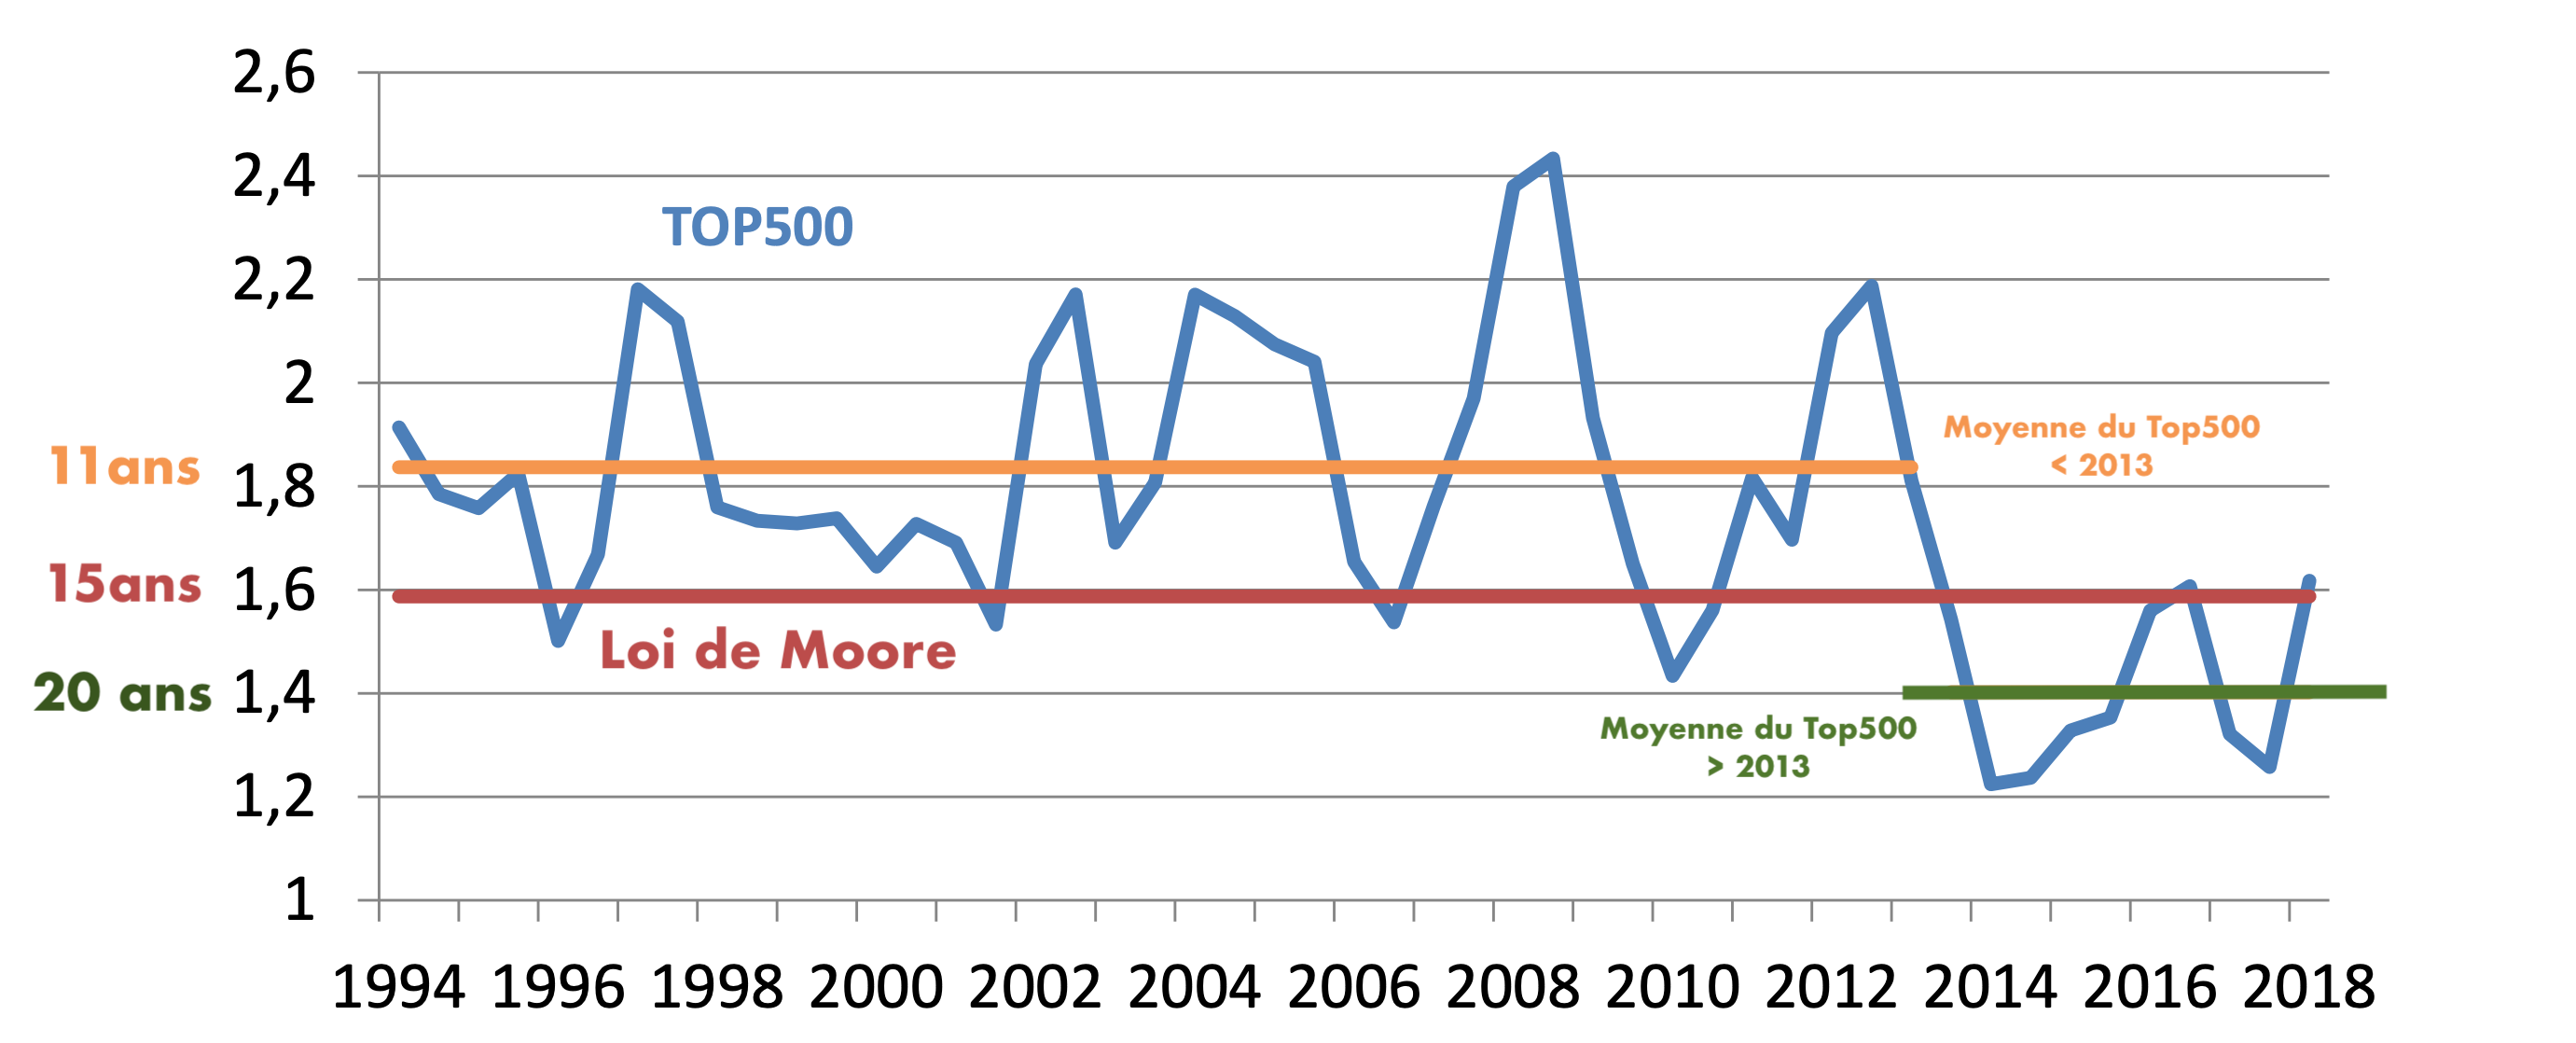
\includegraphics[width=16cm]{images/moore_vs_top500.png}
            \caption{\label{fig:moore_vs_top500}
             Facteur d'évolution annuelle des performances du Top500\protect\footnotemark. Jusqu'à 2013 la performance moyenne du Top500 évoluait d'un facteur 1.8, supérieur à l'évolution prédite par la loi de Moore (facteur 1.6). }
                \end{figure}
            \footnotetext{Graphique inspire de la présentation du Top500 lors de la conférence ISC18 - \textit{Highlights of the 51st TOP500 List}}

        \paragraph{Fin de la validé de la loi de Dennard.} 
                
            Dans l'\aref{sec:denard}, nous avons discuté de l'augmentation de la fréquence des processeurs et introduit \textbf{la loi de Dennard} \cite{Dennard1974}. Ces équations ont assuré l'augmentation de la fréquence des processeurs, de 40\% tous les 2 ans pendant plus de trente ans. À cause des courants de fuite \cite{Wulf1995} augmentant exponentiellement avec la finesse de gravure des transistors, la consommation électrique des processeurs a elle aussi augmenté. Dans la \autoref{sec:denard}, nous expliquons comment la réduction de la taille des transistors et l'augmentation de la fréquence des processeurs augmentent la consommation électrique de circuit. L'énergie utilisée par le processeur étant dissipée sous forme de chaleur, il est devenu très difficile de refroidir ces architectures. De plus, l'énergie nécessaire pour le refroidissement a un impact sur la consommation. Cette limitation physique empêchant d'augmenter la puissance électrique des processeurs est appelée \textit{power wall} \cite{Kuroda2001}.

        \paragraph{Budget.} 
            
            Le prix des supercalculateurs est un frein à la construction de centres toujours plus puissants. Les calculateurs les moins puissants du classement sont généralement ceux dont le budget est le faible. Grâce à l'analyse du Top500, nous pouvons estimer que l'économie est un des freins participant au ralentissement de l'évolution des performances des architectures (voir \autoref{fig:Top500_Poor}). Le décrochage des performances du Top500, autour de 2012, étudié dans la section précédente intervient plus de 4 ans après le décrochage du dernier du classement (en 2008). De plus, on peut étudier la répartition de la performance du Top500 entre les supercalculateurs. En 2004, il fallait agréger les 80 premiers supercalculateurs du classement pour obtenir la moitié de la performance cumulée du Top500. En 2019, il faut seulement cumuler la puissance des 28 premiers. Ceci montre que les plateformes en haut du classement ont tendance à augmenter leur performance plus vite que celles du bas.
            
            
    
            \begin{figure}
            \center
            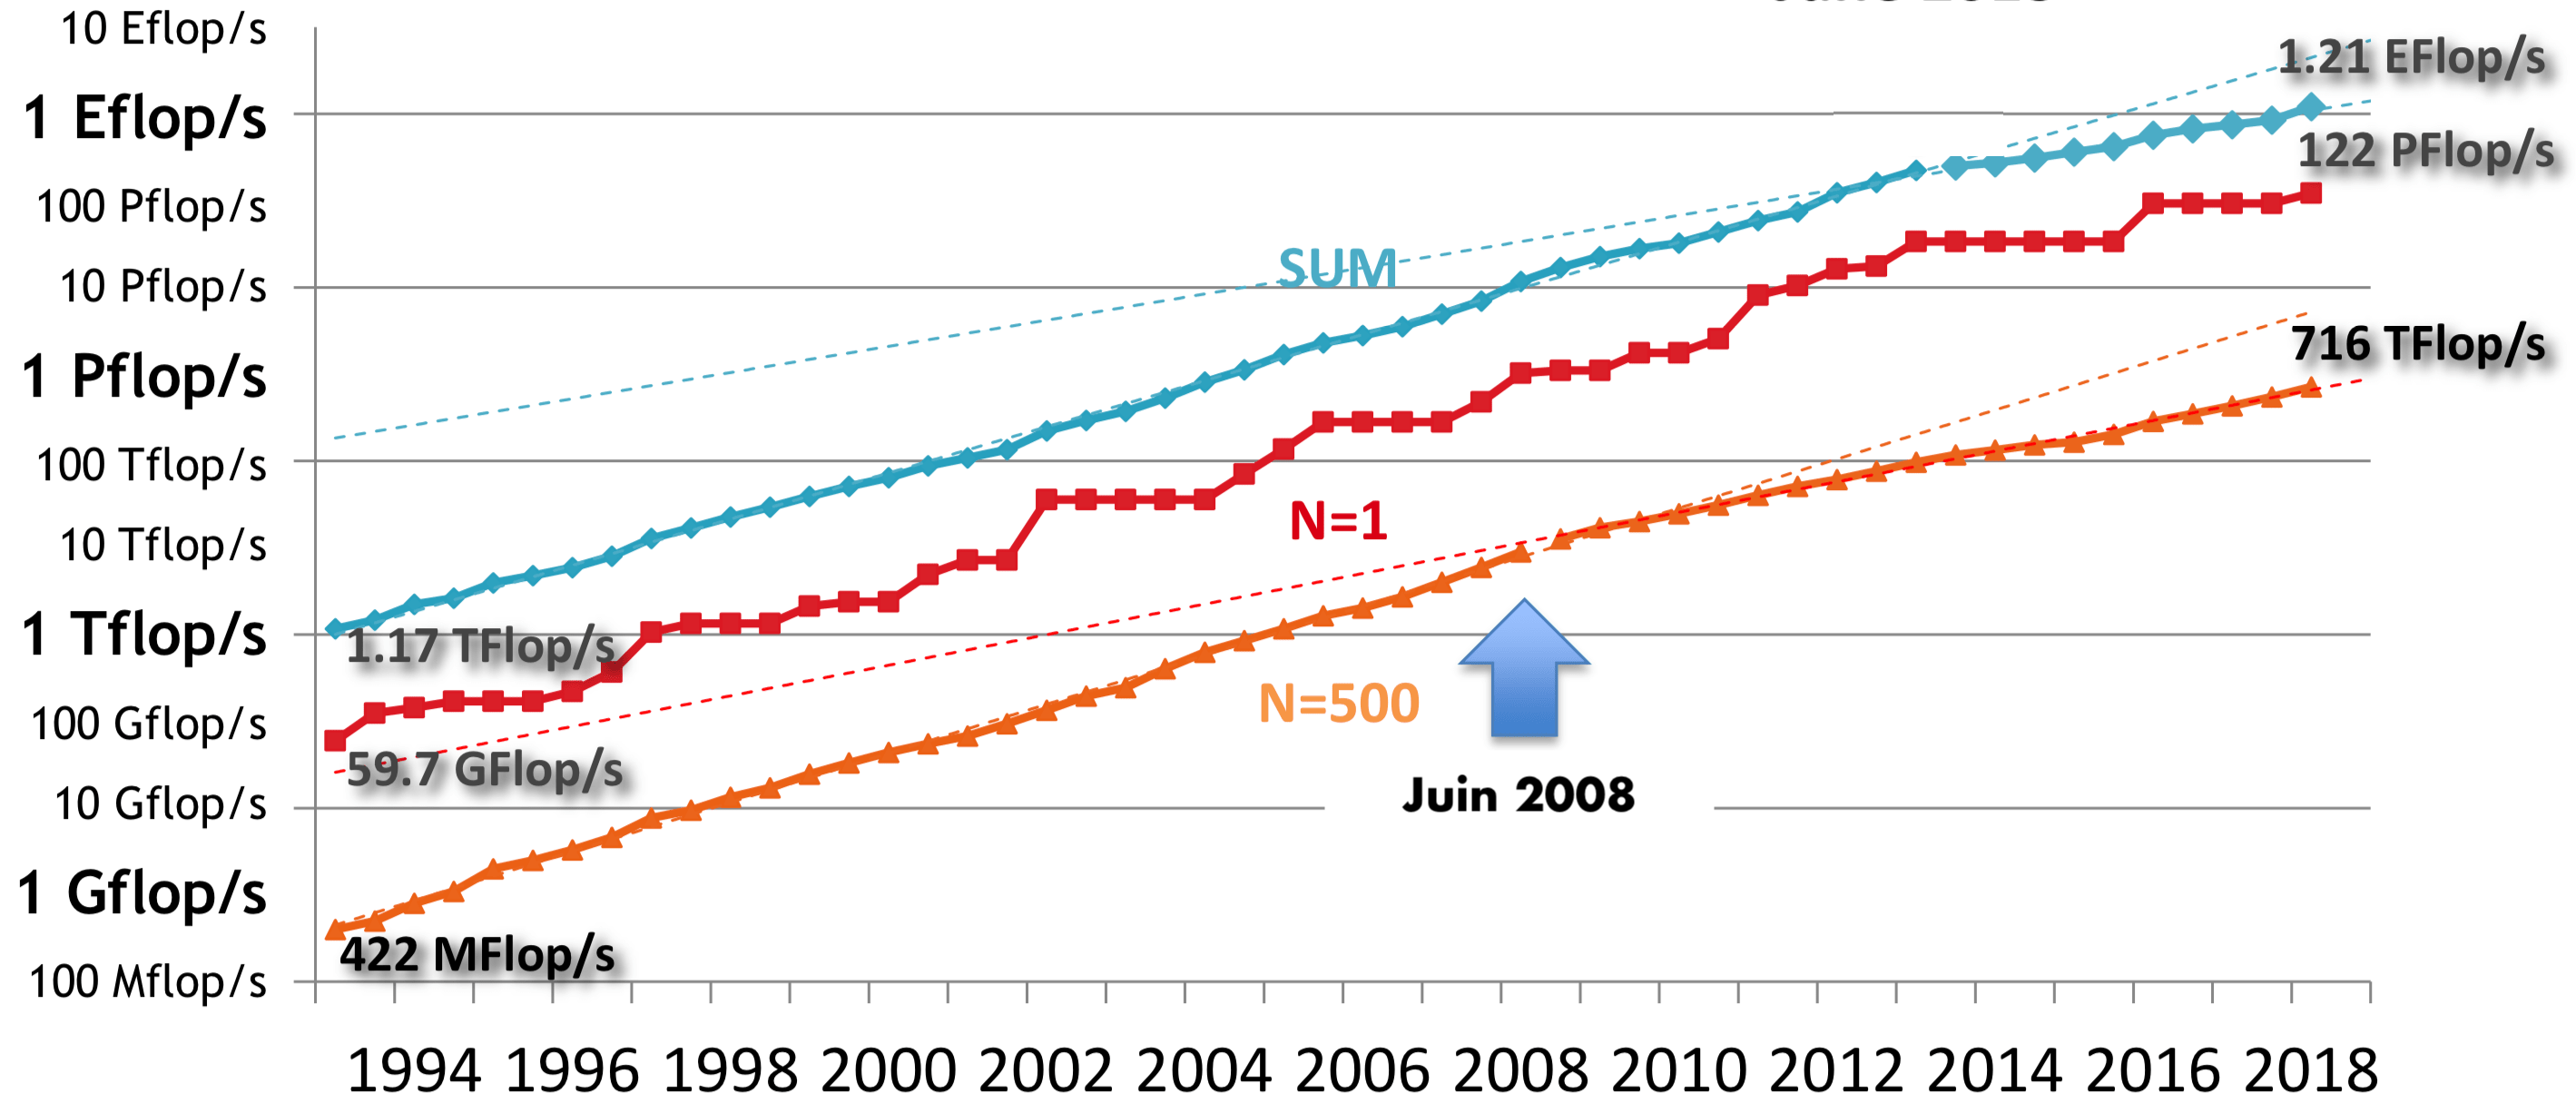
\includegraphics[width=14cm]{images/Top500_Poor.png}
            \caption{\label{fig:Top500_Poor} Évolution des performances du Top500 en \gls{FLOPS} grâce à l'aide du benchmark HPL. Le graphe présente la puissance cumulée des 500 ordinateurs (en bleu), celle du premier (en rouge) et celle du dernier (en orange)\protect\footnotemark.}
            \end{figure}
            \footnotetext{Graphique tiré de \url{https://www.top500.org/news/112019-highlights/}}
    
                
%%%%%%%%%%%%%%%%%%%%%%%%%%%%%%%%%%%%%%%%%%%%%%%%%%%%%%%%%%%%%%%%%%%%%%%%%%%% 
            
        \paragraph{Déséquilibre des microarchitectures.}  
        Si l'utilisation de processeurs multicoeurs a permis de continuer d'augmenter la performance des processeurs malgré la faible évolution des fréquences, l'ajout de coeur a lui aussi atteint ses limites. En effet, comme démontré dans la \autoref{sec:parallele_perf}, l'augmentation des niveaux de parallélisme atteint elle aussi ses limites lorsque les applications contiennent des zones de codes séquentiels. Même des applications comme le benchmark \verb|HPL| sont impactés par \textbf{la loi d'Amdahl}, et l'ajout de coeurs s'est révélé de moins en moins efficace. On remarque sur la \autoref{fig:evo_proc} que le nombre de coeurs a peu évolué ces dix dernières années. Dans l'\aref{sec:memory_wall_gap}, nous discutons de la disparité des évolutions technologiques des processeurs d'une part et des mémoires d'autre part. Cet écart a évolué au fil des années et il est aujourd'hui appelé \textit{mur de la mémoire} \cite{Rojas1997}  (\textit{memory wall} ou \textit{memory gap}). Les premiers processeurs étaient limités par la puissance de calcul, aujourd'hui il est très rare que la performance des applications de calcul haute performance soit limitée par les FPU. L'ajout supplémentaire de coeurs est donc moins bénéfique, car le ratio de bande passante disponible par coeur diminue. 
        Si on regarde l'évolution des performances des différentes parties du système, on peut constater de réelles différences:             
        \begin{itemize}                 
            \item La performance calculatoire des processeurs (le nombre d'opérations flottantes réalisables par cycle) a \textbf{augmenté de 50\%} en moyenne par an.
            \item La bande passante entre le processeur et la mémoire a augmenté de 23\% par an                 
            \item La latence des requêtes mémoires a \textbf{diminué de 4\% } par an                 
            \item La bande passante sur le réseau a \textbf{augmenté de 20\%} par an             
        \end{itemize}
            
            La \autoref{pic:cpuvsmemory2} montre le déséquilibre entre ces deux parties fondamentales des architectures Von Neumann. Ce déséquilibre empêche aujourd'hui le système mémoire de transférer les données suffisamment rapidement pour que la totalité des unités de calculs soit constamment active. Pourtant, 50\% des broches d'un processeur récent sont allouées au système mémoire. Ainsi, bien que les performances de calculs des processeurs s'améliorent, les applications ne peuvent pas en bénéficier. La plupart des supercalculateurs atteignent rarement une efficacité de 80\% sur une application simple comme Linpack \cite{Dongarra2003}. Pour des applications réelles, cette efficacité est encore plus faible, parfois inférieure à 10\% \cite{Oliker2005}.
            
            \begin{figure}             \center             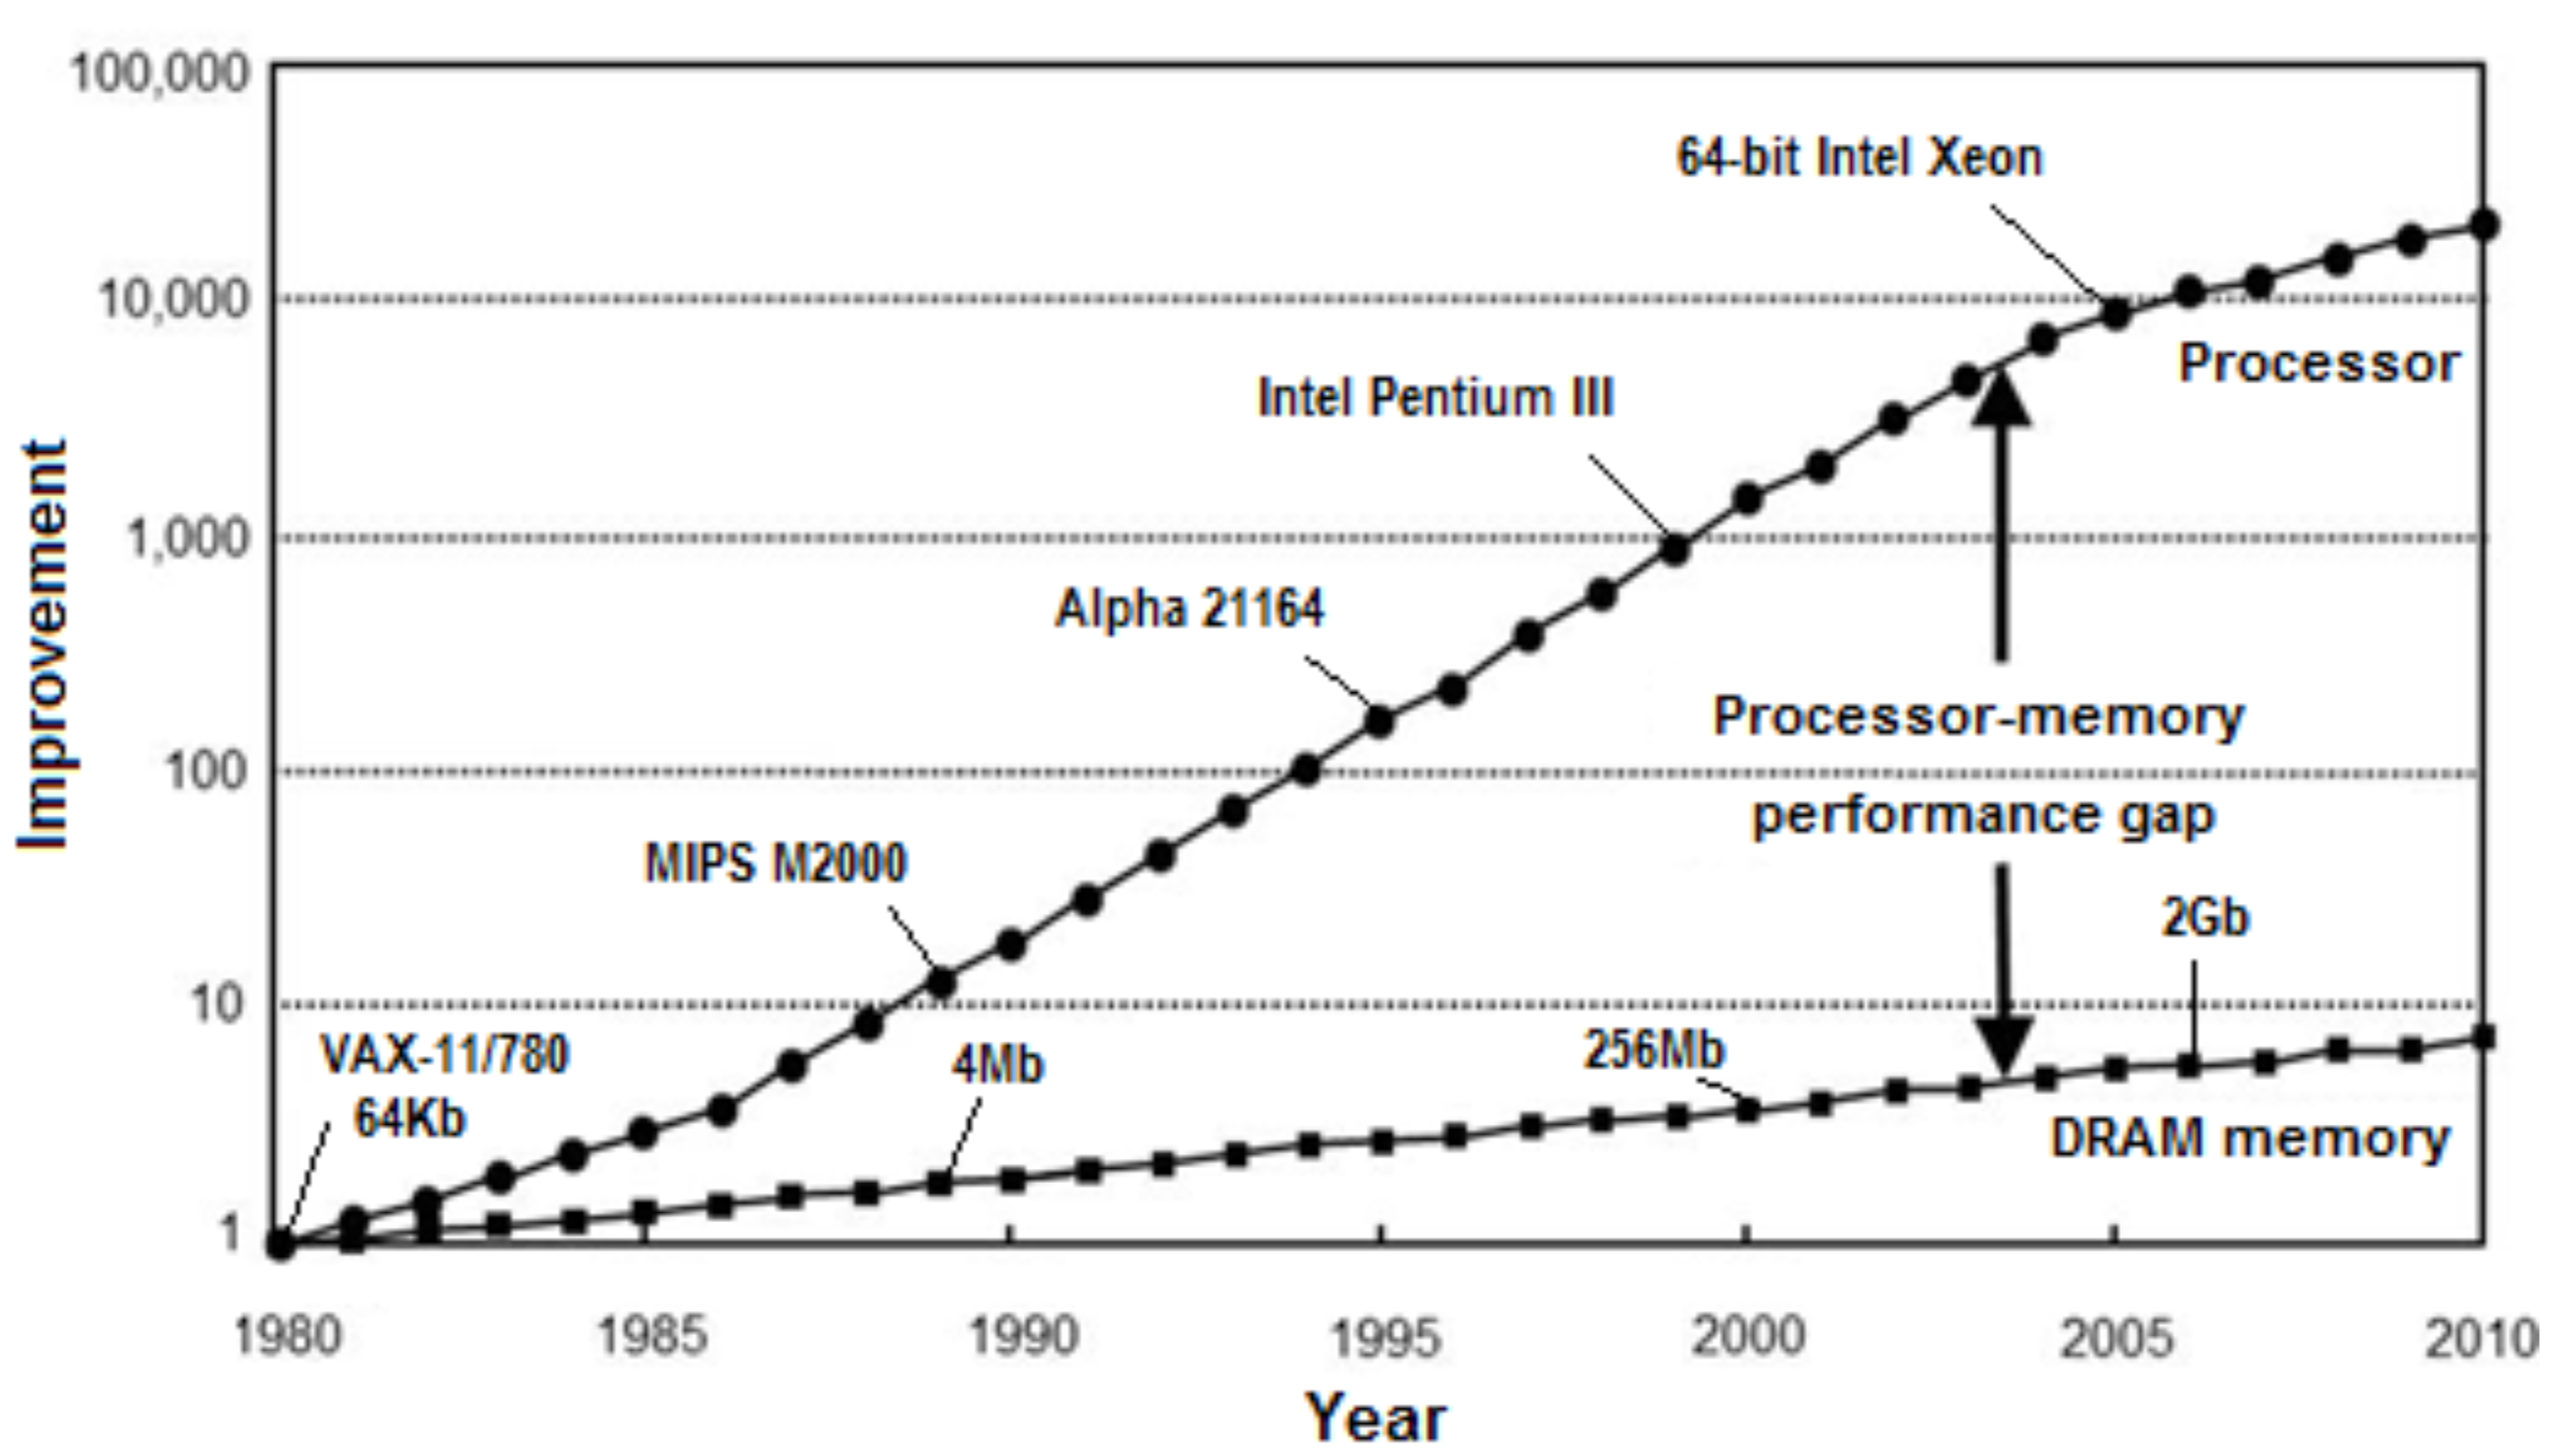
\includegraphics[width=10cm]{images/cpu_cpu_vs_memory.png}             \caption{\label{pic:cpuvsmemory2} Progression de la performance des processeurs et des mémoires. La performance de plusieurs générations de processeurs a été mesurée à l'aide du benchmark SPECint \cite{Efnusheva2017ASO}. La performance mémoire est représentée par la latence des accès mémoire (CAS et RAS) des mémoires DRAM.}
            \end{figure}
            
            Le déséquilibre des microarchitectures se fait d'autant plus ressentir lorsque des centaines de serveurs sont réunis. La \autoref{fig:unbalance_flop_io} montre l'évolution de la puissance des serveurs et du débit mémoire des 10 premiers supercalculateurs du Top500. Grâce aux évolutions des processeurs (voir \autoref{sec:proc_evo_2012}) et l'utilisation des GPUs, la puissance des serveurs a été multipliée en moyenne par 65 entre 2010 et 2018 (courbe bleue). Pendant la même période, le débit des communications inter serveur n'a lui augmenté que d'un facteur 4.8 (courbe rouge). Ainsi, le ratio entre la puissance de calcul des serveurs et le débit de communication (byte par \gls{FLOP}) n'a fait que diminuer. Entre 2017 et 2018, ce ratio a diminué d'un facteur 8 pour les deux premiers supercalculateurs du Top500 (respectivement Sunway Taihulight et Summit). Pour des applications nécessitant de grandes communications interserveur, ce ratio très faible les empêche d'atteindre plus d’une fraction de la performance disponible.
            
            \begin{figure}             \center             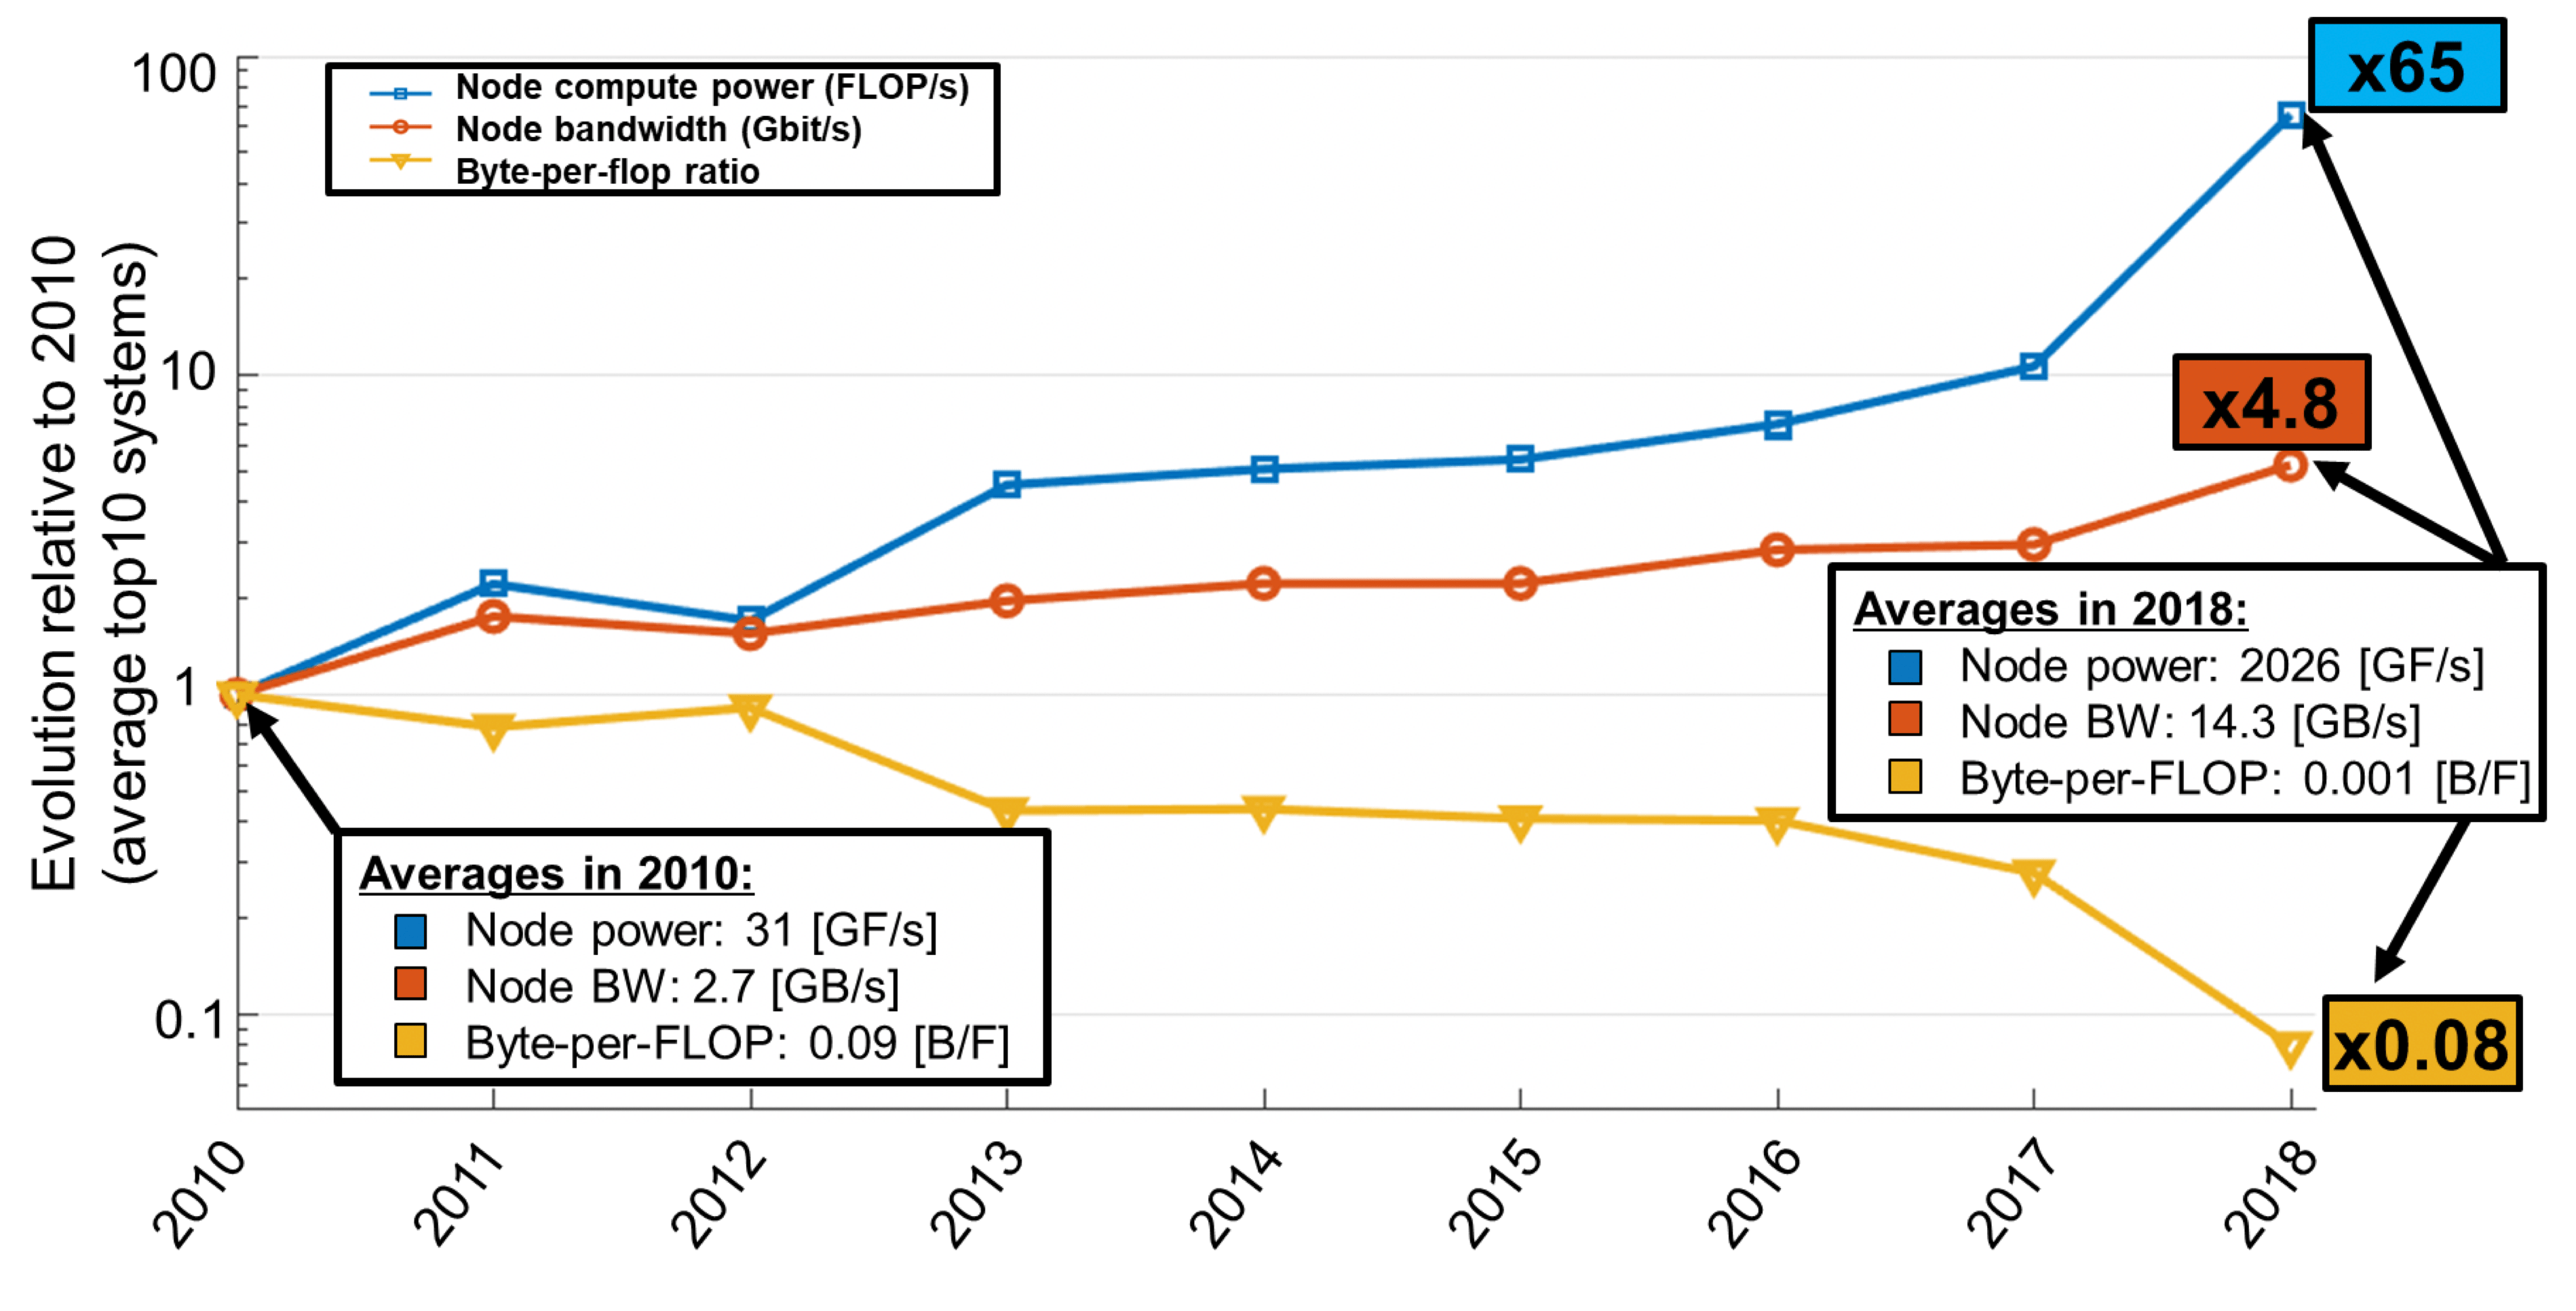
\includegraphics[width=12cm]{images/unbalance_flop_io.png}             \caption{\label{fig:unbalance_flop_io}Évolution des 10 premiers supercalculateurs du Top500 de 2010 à 2018: la puissance de calcul des serveurs (FLOP/s) en bleu, le débit de communication entre les serveurs (Gbit/s) en orange, ainsi que le ratio entre ces deux caractéristiques (byte par \gls{FLOP}) en jaune. (graphique tiré de la conférence IPDPS 2018 \cite{Bergman2018})}             \end{figure}
 
 
\subsection{Le futur du HPC}
%%%%%%%%%%%%%%%%%%%%%%%%%%%%%%%%%%%%%%%%%%%%%%%%%%%%%%%%%%%%%%%%%%%%%%%%


    \begin{fancyquotes}
    Peu importe la puissance qu'atteindront les processeurs, le logiciel trouvera toujours une façon d'utiliser cette puissance. Construisez un processeur 10 fois plus rapide, et la partie logiciel trouvera toujours 10 fois plus à faire (ou le fera 10 fois moins efficacement)  \cite{Sutter2005}.
    \end{fancyquotes}
 
    \subsubsection{Situation du HPC en 2020}
    %%%%%%%%%%%%%%%%%%%%%%%%%%%%%%%%%%%%%%%%%%%%%%%%%%%%%%%%%%%%%%%%%%%%%%%%

   
        %EVO DES PERFORMANCES IT
        
        La performance des supercalculateurs et des technologies de l'information n'a fait qu'augmenter au cours de ces 30 dernières années. Une montre connectée récente apporte une puissance de calcul deux fois supérieure à celle du supercalculateur Cray-2, le plus puissant des supercalculateurs de 1985. Un GPU moderne tel que le GPU Nvidia V100 délivrant une puissante de 7.5 téraFLOPS ($10^{12}$ \gls{FLOPS}) serait classé à la 30e place du Top500 de 1994.

        %HPC: PLUS QUE DU CALCUL, UN MODE DE VIE
            
        L'évolution des performances des matériels informatiques a largement transformé le mode de vie de nos sociétés. Les produits du HPC sont présents dans nos vies quotidiennes: nous nous déplaçons grâce à l'essence extraite à l'aide de la modélisation des fonds marins, lorsque nous consultons la météo ou lorsque nous ingérons un médicament. Le HPC a un réel impacte sur nos vies, les rendant plus sécurisées en prévoyant précisément des catastrophes naturelles. 
        Le HPC est un outil inhabituel, car il ne se limite pas à un domaine particulier. La majorité des domaines scientifiques ont recours à des calculateurs. 
        %IL Y A UNE DEMANDE DE PLUS DE CALCUL
  
        Suite à la forte évolution de la performance des supercalculateurs, nous pouvons nous demander s'il est nécessaire de continuer à construire des infrastructures toujours plus puissantes. La variété et la complexité des problèmes qui peuvent être traités dépendent directement de la puissance de calcul disponible. L’apprentissage profond (\textit{deep learning}) en est un bon exemple. Dès 1989, Yann LeCun améliorait déjà la rétropropagation \cite{Treibig2012a} et utilisait les réseaux neuronaux convolutionnels \cite{LeCun1989}. Mais à cette époque les GPGPU n'étaient pas disponibles et les CPU étaient loin d'être assez puissants pour exécuter ces algorithmes, même sur les données limitées disponibles à cette époque. Dans les années 2010, les GPU sont devenus suffisamment puissants pour permettre l'exécution de ces algorithmes.
        
        
        La mise au point de plateformes plus puissantes va permettre aux entreprises d'être plus compétitives et aux équipes de recherches de réaliser de nouvelles découvertes. Un grand nombre de domaines scientifiques vont pouvoir profiter de telles puissances de calculs: découverte de nouveaux matériaux, simulations de réactions chimiques ou encore pour analyser les résultats d'expériences lourdes comme celles réalisées au Grand collisionneur de hadrons \cite{10.1007/978-3-319-67630-2_52}. La recherche pour le climat va aussi bénéficier de telles architectures et permettre de comprendre les dérèglements climatiques, anticiper la hausse des océans et élaborer de meilleurs modèles. Les simulations permettront également d'améliorer l'efficacité et la sécurité des réacteurs nucléaires \cite{Simon2007}. En astrophysique, elles permettront d'étudier des phénomènes encore incompris comme la formation des trous noirs \cite{10.1007/978-3-642-38750-0_2}. L'accès à des infrastructures plus puissantes permettra de poursuivre les avancées réalisées dans le domaine de la physique quantique. Ces découvertes pourront permettre de construire d'autres plateformes de calculs appelées ordinateurs quantiques.
        
         
    \subsubsection{Nécessité de construire des plateformes plus puissantes}\label{sec:3_motivations}
    %%%%%%%%%%%%%%%%%%%%%%%%%%%%%%%%%%%%%%%%%%%%%%%%%%%%%%%%%%%%%%%%%%%%%%%%

        \begin{fancyquotes}
        La taille des données double tous les deux ans, et d'ici 2020, les données que nous générons et copions annuellement atteindront 44 Zettabytes ($10^{21}$ bytes) \cite{Zhang2017}.
        \end{fancyquotes}
    
        Aujourd'hui, de nombreuses applications sont prêtes, mais ne peuvent pas être exécutées en un temps raisonnable avec les moyens de calculs disponibles. Actuellement il est possible de simuler des réactions chimiques de quelques nanosecondes et sur de petits volumes. Avec la construction de supercalculateurs plus puissants, il sera possible de réaliser des simulations plus longues et plus précises. Nous discutons dans cette section de trois facteurs importants qui motivent la nécessité de poursuivre le développement de plateformes plus performantes que celles actuellement en notre possession: l'explosion du volume de données à traiter, la complexification des analyses et le besoin d'obtenir des résultats rapidement.

        
        \paragraph{Tsunami de données.} 
            
            Suite aux évolutions des technologies des semi-conducteurs, nous assistons depuis le début des années 2010 à l'explosion des quantités de données générées (voir \autoref{fig_edl_bigdata}). Grâce aux nanotechnologies, il est possible de produire des capteurs à très faible coût. La consommation électrique de ces matériels étant faible, ces capteurs sont installés partout. L’Internet des Objets (IOT) interconnecte ces milliers de capteurs pour générer de grands volumes de données (\textit{big data}).  Les évolutions récentes de la domotique ont permis d'installer des capteurs dans toute la maison: que ce soit pour gérer les lumières, le chauffage, l'ouverture des volets ou même l'allumage de la cafetière. En 2018, Ericsson comptait plus de 5 milliards d'abonnés au téléphone dans le monde\footnote{Source: \url{https://www.usinenouvelle.com/article/5-4-milliards-d-abonnes-au-telephone-mobile-dans-le-monde.N739439}}. Ces téléphones peuvent aujourd'hui suivre nos moindres faits et gestes, générant de grandes quantités de données. Celles-ci peuvent ensuite être utilisées par différentes applications pour étudier les déplacements des habitants d'une ville ou proposer des annonces ciblées. Les villes elles-mêmes se sont dotées de milliers de capteurs permettant le développement de nombreuses applications comme le suivi du trafic routier \cite{bonhomme:hal-01334670}, l'utilisation des transports en commun, ou de suivre le recyclage des déchets dans un quartier \cite{Rebelles2018}. Ce grand volume de données produit aujourd'hui et qui va s'intensifier dans les années futures est le principal challenge des systèmes d'informations.
        
              
            \begin{figure}
            \center
            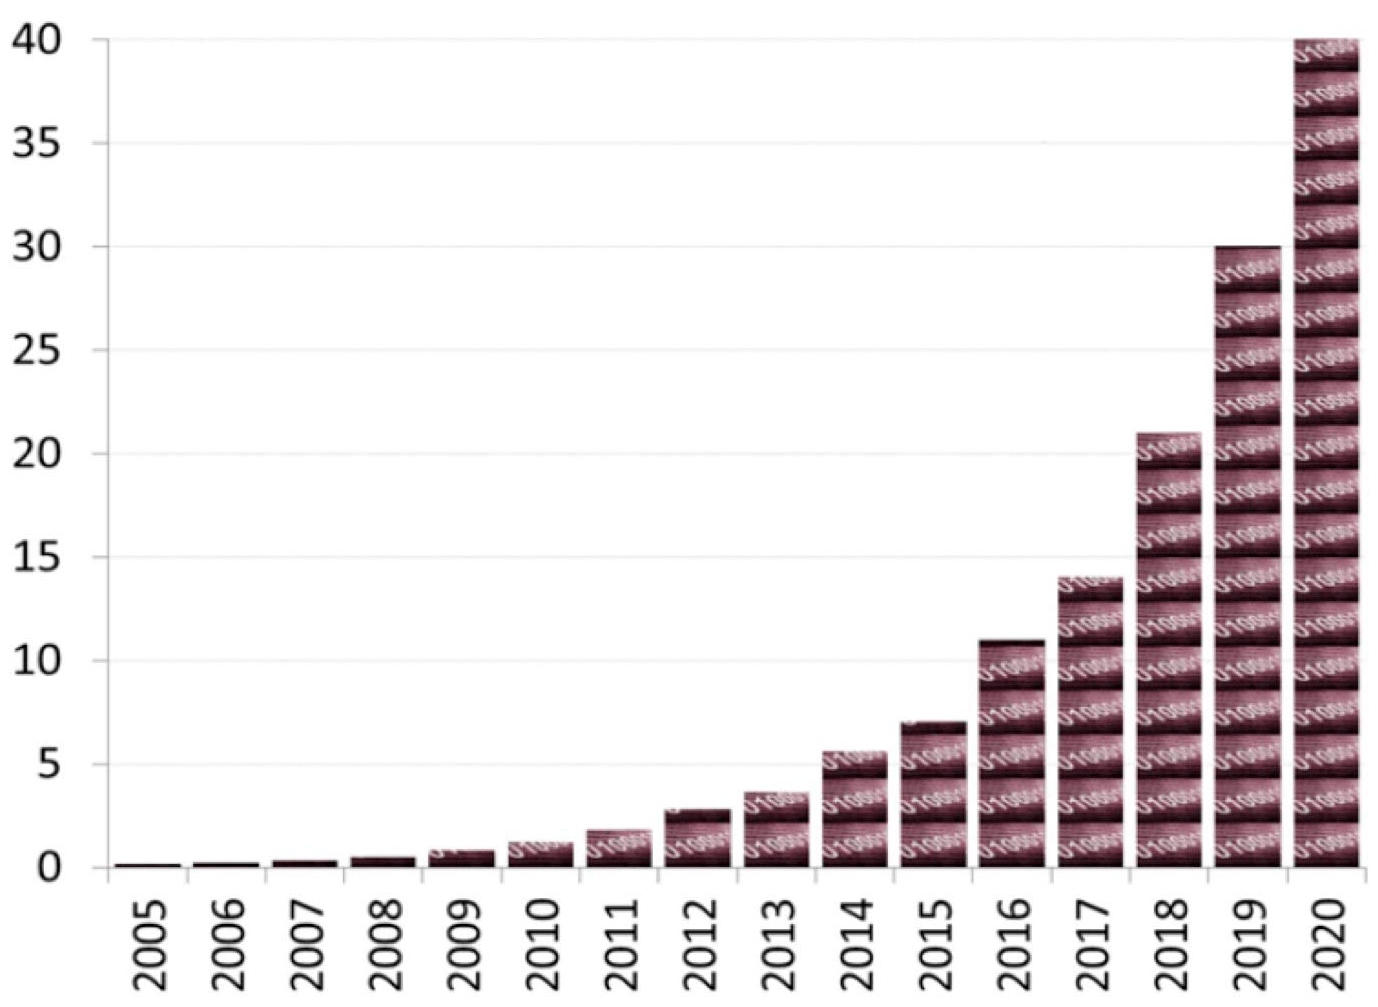
\includegraphics[width=10cm]{images/edl_bigdata.png}
            \caption{\label{fig_edl_bigdata} Le volume de données généré chaque année devrait atteindre 40 Zettabytes en 2020 \cite{Simoudis2016}}
            \end{figure}
        
        

            
        \paragraph{Complexité des calcus.} 
             Aujourd'hui, la valeur ne provient plus de la capacité à produire ces données, mais de la capacité d'en extraire une valeur avec des algorithmes de \textit{big data} et d'apprentissage machine. Les algorithmes d'intelligence artificielle nécessitent d'être entraînés sur des jeux de données pour pouvoir ensuite prendre les décisions adaptées. En 2018, OpenAI a constaté que la puissance de calcul utilisée pour entraîner les plus grands modèles d'IA avait doublé tous les 3,4 mois depuis 2012 (voir \autoref{fig_edl_ai_compute}). Dans le domaine de la santé, de telles infrastructures pourront permettre d'extraire et analyser toutes les informations de millions de patients atteints de maladies grâves.  Il sera alors possible de mieux comprendre les symptômes menant au développement d'un cancer ou d'une maladie cardiaque. 
             Pour obtenir des résultats dans des temps raisonnables, ces applications nécessitent d'avoir accès à des plateformes plus puissantes de plusieurs facteurs que celles existant actuellement. Avec l'analyse des données obtenues grâce aux montres connectées, il sera alors possible d'anticiper les maladies cardiaques.
             
            \begin{figure}
            \center
            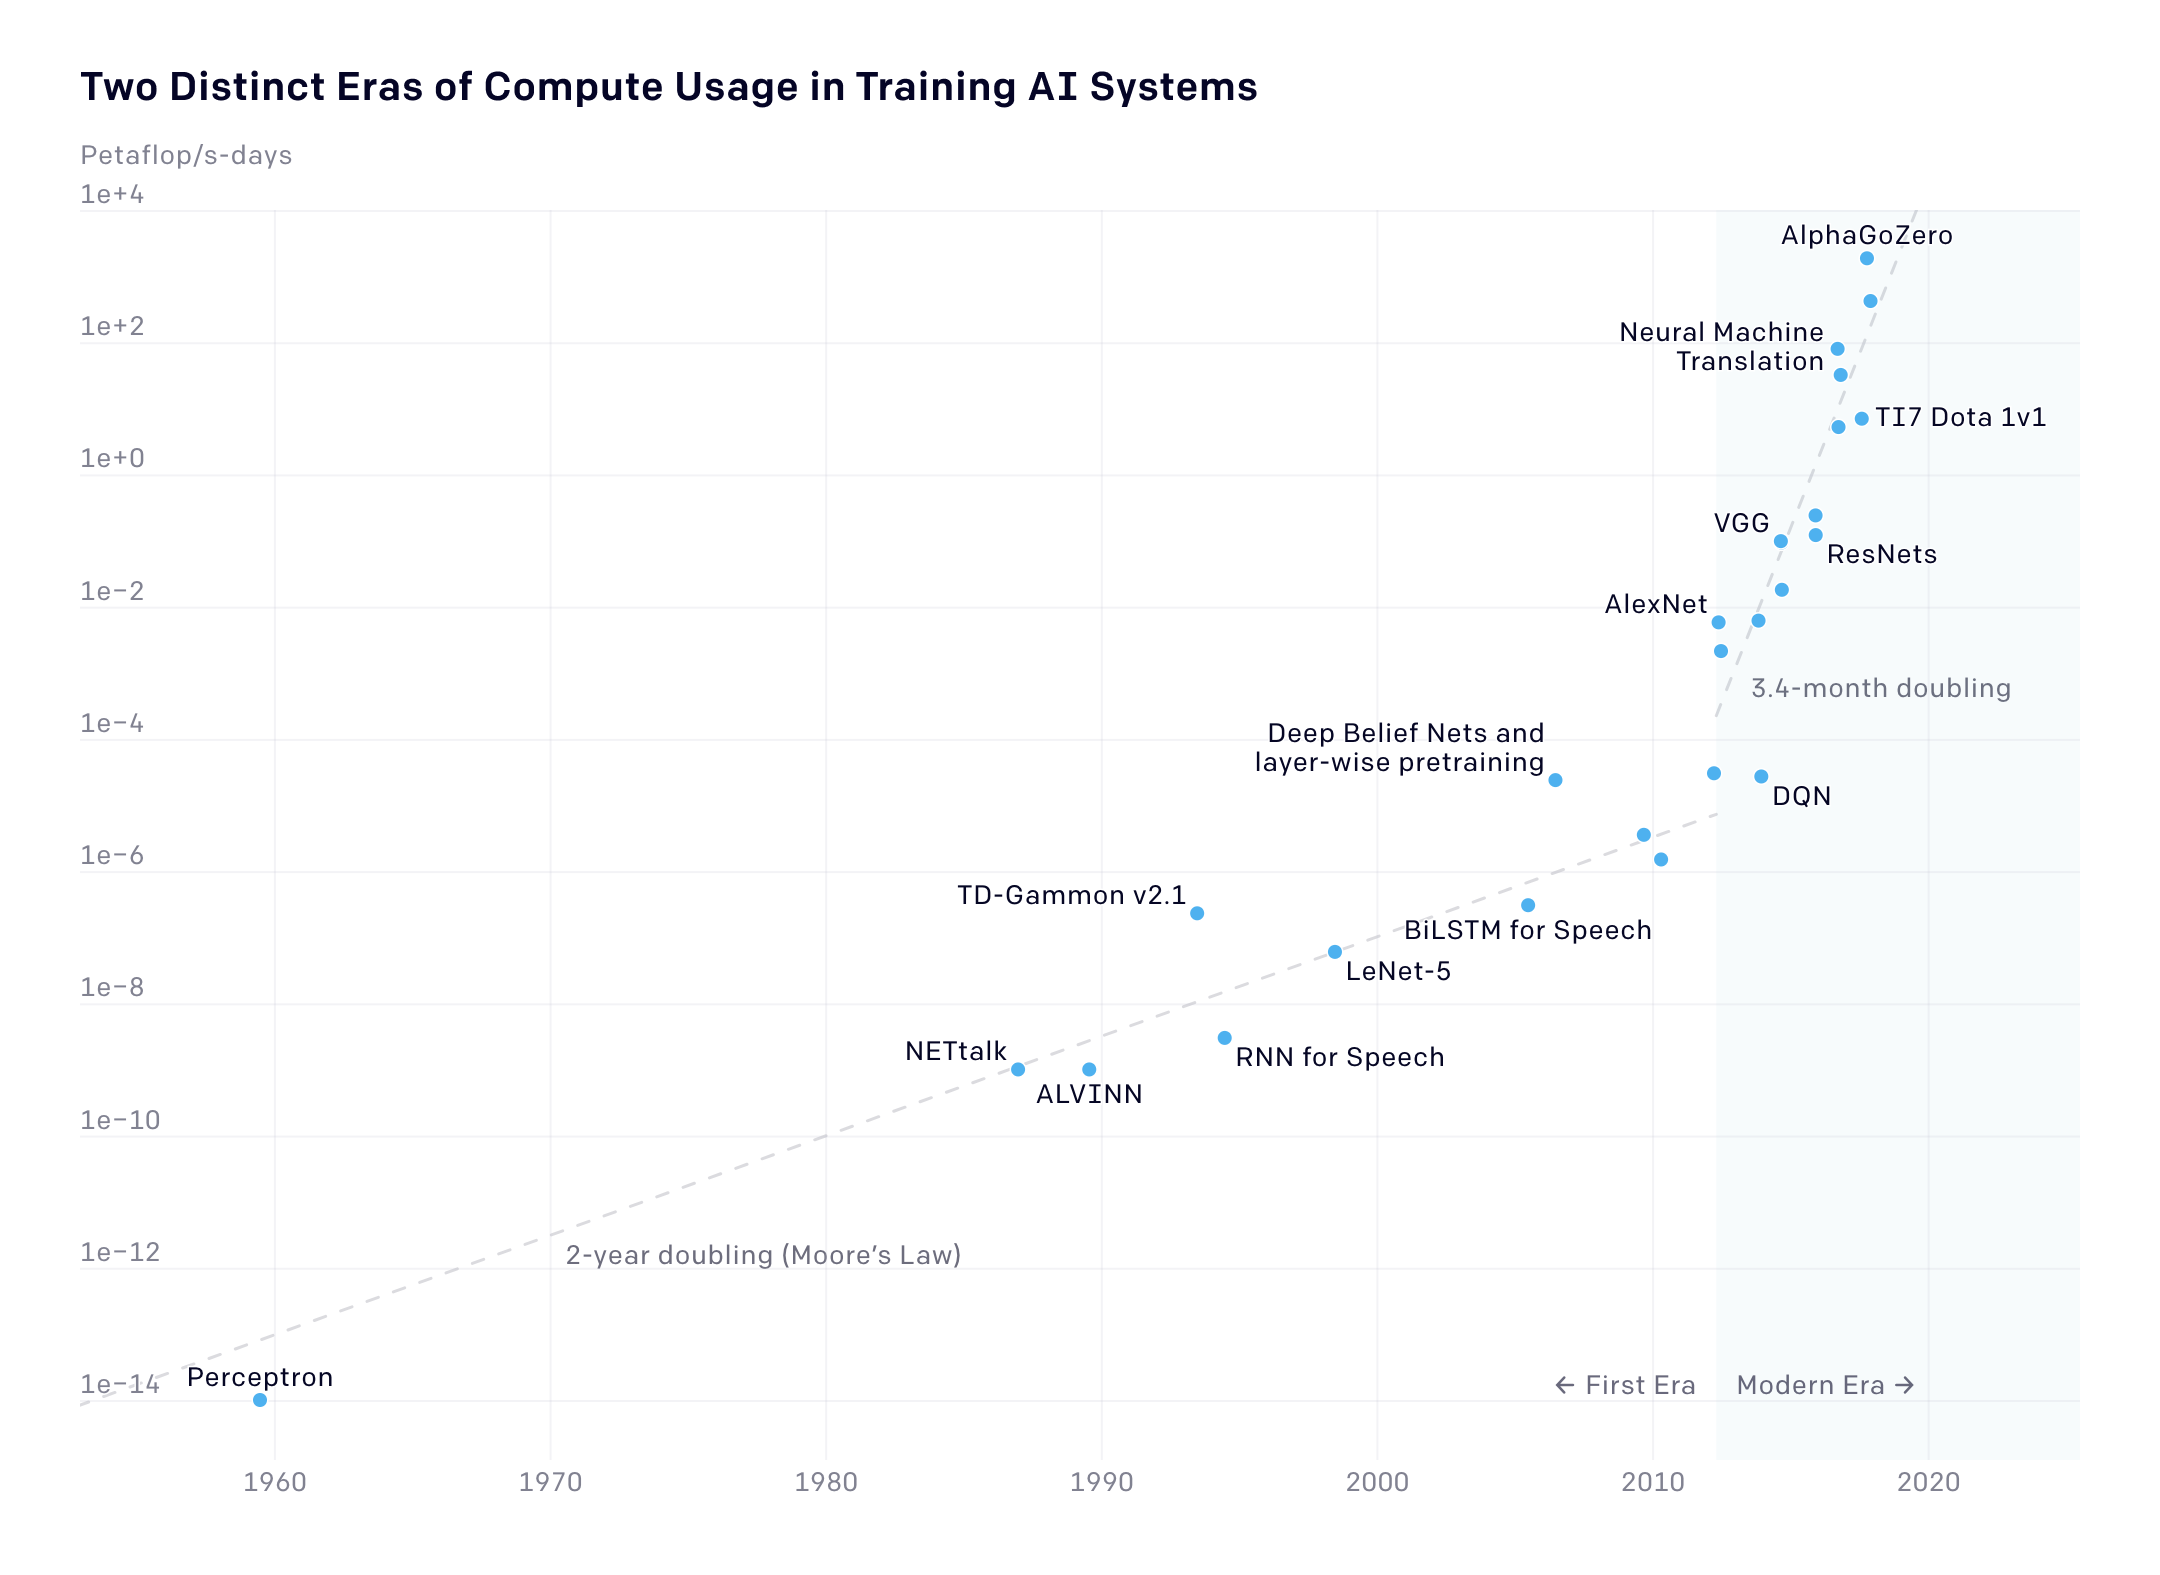
\includegraphics[width=14cm]{images/edl_ai_compute.png}
            \caption{\label{fig_edl_ai_compute} Quantité totale de calcul (en pétaFLOPS ($10^{15}$ \gls{FLOPS})) nécessaire chaque jour pour entraîner les différents réseaux de neurones \cite{amodei2ai}.}
            \end{figure}

        \paragraph{Temps de traitement.} 
        
            La troisième raison qui motive le développement de nouvelles plateformes plus puissantes est de réduire le temps d'exécution des applications. Une fois la donnée produite, sa valorisation diminue dans le temps. La météo est un très bon exemple d'application ne pouvant pas excéder un certain temps de traitement si les prédictions veulent être données suffisamment rapidement. Par exemple, pour permettre aux voitures connectées d'identifier un danger, l'action correspondante doit être prise le plus rapidement possible. La possibilité d'envoyer les données à traiter à un supercalculateur n'est alors pas envisageable. L'accès à des plateformes plus puissantes est alors nécessaire pour traiter cette quantité de données dans des temps raisonnables. En plus d'améliorer les performances des supercalculateurs, l'architecture complète des plateformes doit être repensée. Pour traiter efficacement le volume de données générées, plusieurs travaux montrent qu'il est indispensable de repenser notre façon de stocker, déplacer et analyser ces données \cite{Saltz2018, Chen2014, Nahrstedt2017, GeoffreyFoxJhaShantenu2015}.
  
 
    \subsubsection{Exascale}\label{sec:exascale}
    %%%%%%%%%%%%%%%%%%%%%%%%%%%%%%%%%%%%%%%%%%%%%%%%%%%%%%%%%%%%%%%%%%%%%%%%
        
      
        %Exascale Definition maison             
        
        Le terme \gls{exascale} est utilisé pour définir la prochaine génération de supercalculateurs capable d'atteindre une performance de \gls{exaFLOPS}. Cette performance devra être mesurée à l'aide du benchmark High-Performance Linpack (HPL \cite{Dongarra2003}). En effet, certains supercalculateurs sont déjà capables d'atteindre de telles performances sur des applications plus simples. En 2018 le supercalculateur Summit était capable d'exécuter $1.2 * 10^{18}$ opérations par seconde. L'application utilisée était une application d'apprentissage en profondeur utilisée pour étudier les déchets nucléaires.  Cette application n'utilise que des opérations en simple précision. Le même supercalculateur a pu atteindre une performance de $3.3 \times 10^{18}$ opérations sur une application d'analyse de données, elle aussi en simple précision \cite{Bergman2018}.
         \footnote{\url{https://insidehpc.com/2019/11/deep-learning-on-summit-supercomputer-powers-insights-for-nuclear-waste-remediation/}}. 
        
        Dans la littérature, il est courant d'utiliser le terme \textit{exascale} pour désigner cette nouvelle génération de plateformes 10 fois plus puissantes que les supercalculateurs les plus puissants actuels et 30 fois plus puissants que la moyenne du Top500 de novembre 2019 (33 pétaFLOPS). Le rapport commandé par le département de l'énergie américain en 2014 \cite{Lucas2014} souligne que ce terme ne fait pas référence à la puissance obtenue par le benchmark HPL, mais bien à une plateforme avec 1000 fois plus de capacité que les supercalculateurs existant alors. Dans ces travaux de thèse, nous suivons la même démarche et utilisons le terme exascale pour désigner la plateforme qui permettra d'obtenir les performances souhaitées. La plateforme ne concerne pas seulement le supercalculateur, mais toute la chaîne de traitement de données, depuis sa création jusqu'à son traitement.


\subsection{Défis à relever pour l'élaboration d'une plateforme exascale} \label{sec:challenges}
%%%%%%%%%%%%%%%%%%%%%%%%%%%%%%%%%%%%%%%%%%%%%%%%%%%%%%%%%%%%%%%%%%%%%%%%

    %La course à peta etait dure
        
    Jusqu'à aujourd'hui, quand une piste d'évolution venait à s'épuiser, comme l'évolution de la fréquence des processeurs, d'autres améliorations venaient alors y pallier (augmentation du nombre de coeurs). Dans la \autoref{sec:Top500}, nous avons discuté des principaux freins ayant ralenti l'évolution des performances des supercalculateurs ces 8 dernières années. Depuis plusieurs années, de nombreuses études \cite{Shalf2010, bergman2008exascale, Bergman2011} prédisent les principaux challenges à relever pour la construction d'une plateforme exascale. La plus citée d'entre elles est l'étude menée par le département de l'énergie américain \cite{Lucas2014} qui décrit les dix principaux challenges à relever. Ce rapport met en lumière les nombreuses difficultés que l'industrie rencontre et montre que celles-ci touchent toutes les parties des centres de données (\textit{data center)}): l'énergie, les technologies mémoire et d'interconnexion, la programmation, la gestion ou encore la capacité des applications à utiliser la totalité de la puissance disponible. 
    Il est aussi indiqué que pour construire une telle plateforme dans des coûts financiers et des consommations électriques raisonnables, les dernières avancées technologiques des domaines cités précédemment doivent être intégrées. Le travail de la thèse a en partie été motivé par ces challenges présentés dans les études citées ci-dessus. Dans cette section nous présentons en détail les six principales difficultés que nous avons identifiées. 

    \subsubsection{Les coûts}\label{sec:edl_chal_prix}
    %%%%%%%%%%%%%%%%%%%%%%%%%%%%%%%%%%%%%%%%%%%%%%%%%%%%%%%%%%%%%%%%%%%%%%%%
    %%%%%%%%%%%%%%%%%%%%%%%%%%%%%%%%%%%%%%%%%%%%%%%%%%%%%%%%%%%%%%%%%%%%%%%%

    %MOORE et Transistor $
    
        Dans la \autoref{sec:end_mooore} nous avons expliqué comment la fin de la loi de Moore avait impacté l'évolution des performances des supercalculateurs. Bien que souvent oublié, il est important de rappeler que cette loi est avant tout une loi économique.
        Grâce à l'évolution des procédés de gravure, le nombre de transistors a pu doubler tous les deux ans pendant plus de trente ans alors que le coût des investissements dans les fonderies n'augmentait que de 30\% sur la même période. Cette évolution des prix des fonderies porte le nom de \textit{seconde loi de Moore} ou loi de Rock. À cause des nombreux investissements nécessaires pour développer les nouvelles générations de fonderies nous remarquons que le nombre de transistors achetable pour un budget donné n'évolue plus (voir \autoref{fig:edl_moore_dollars}).
    
        \begin{figure}
        \center
        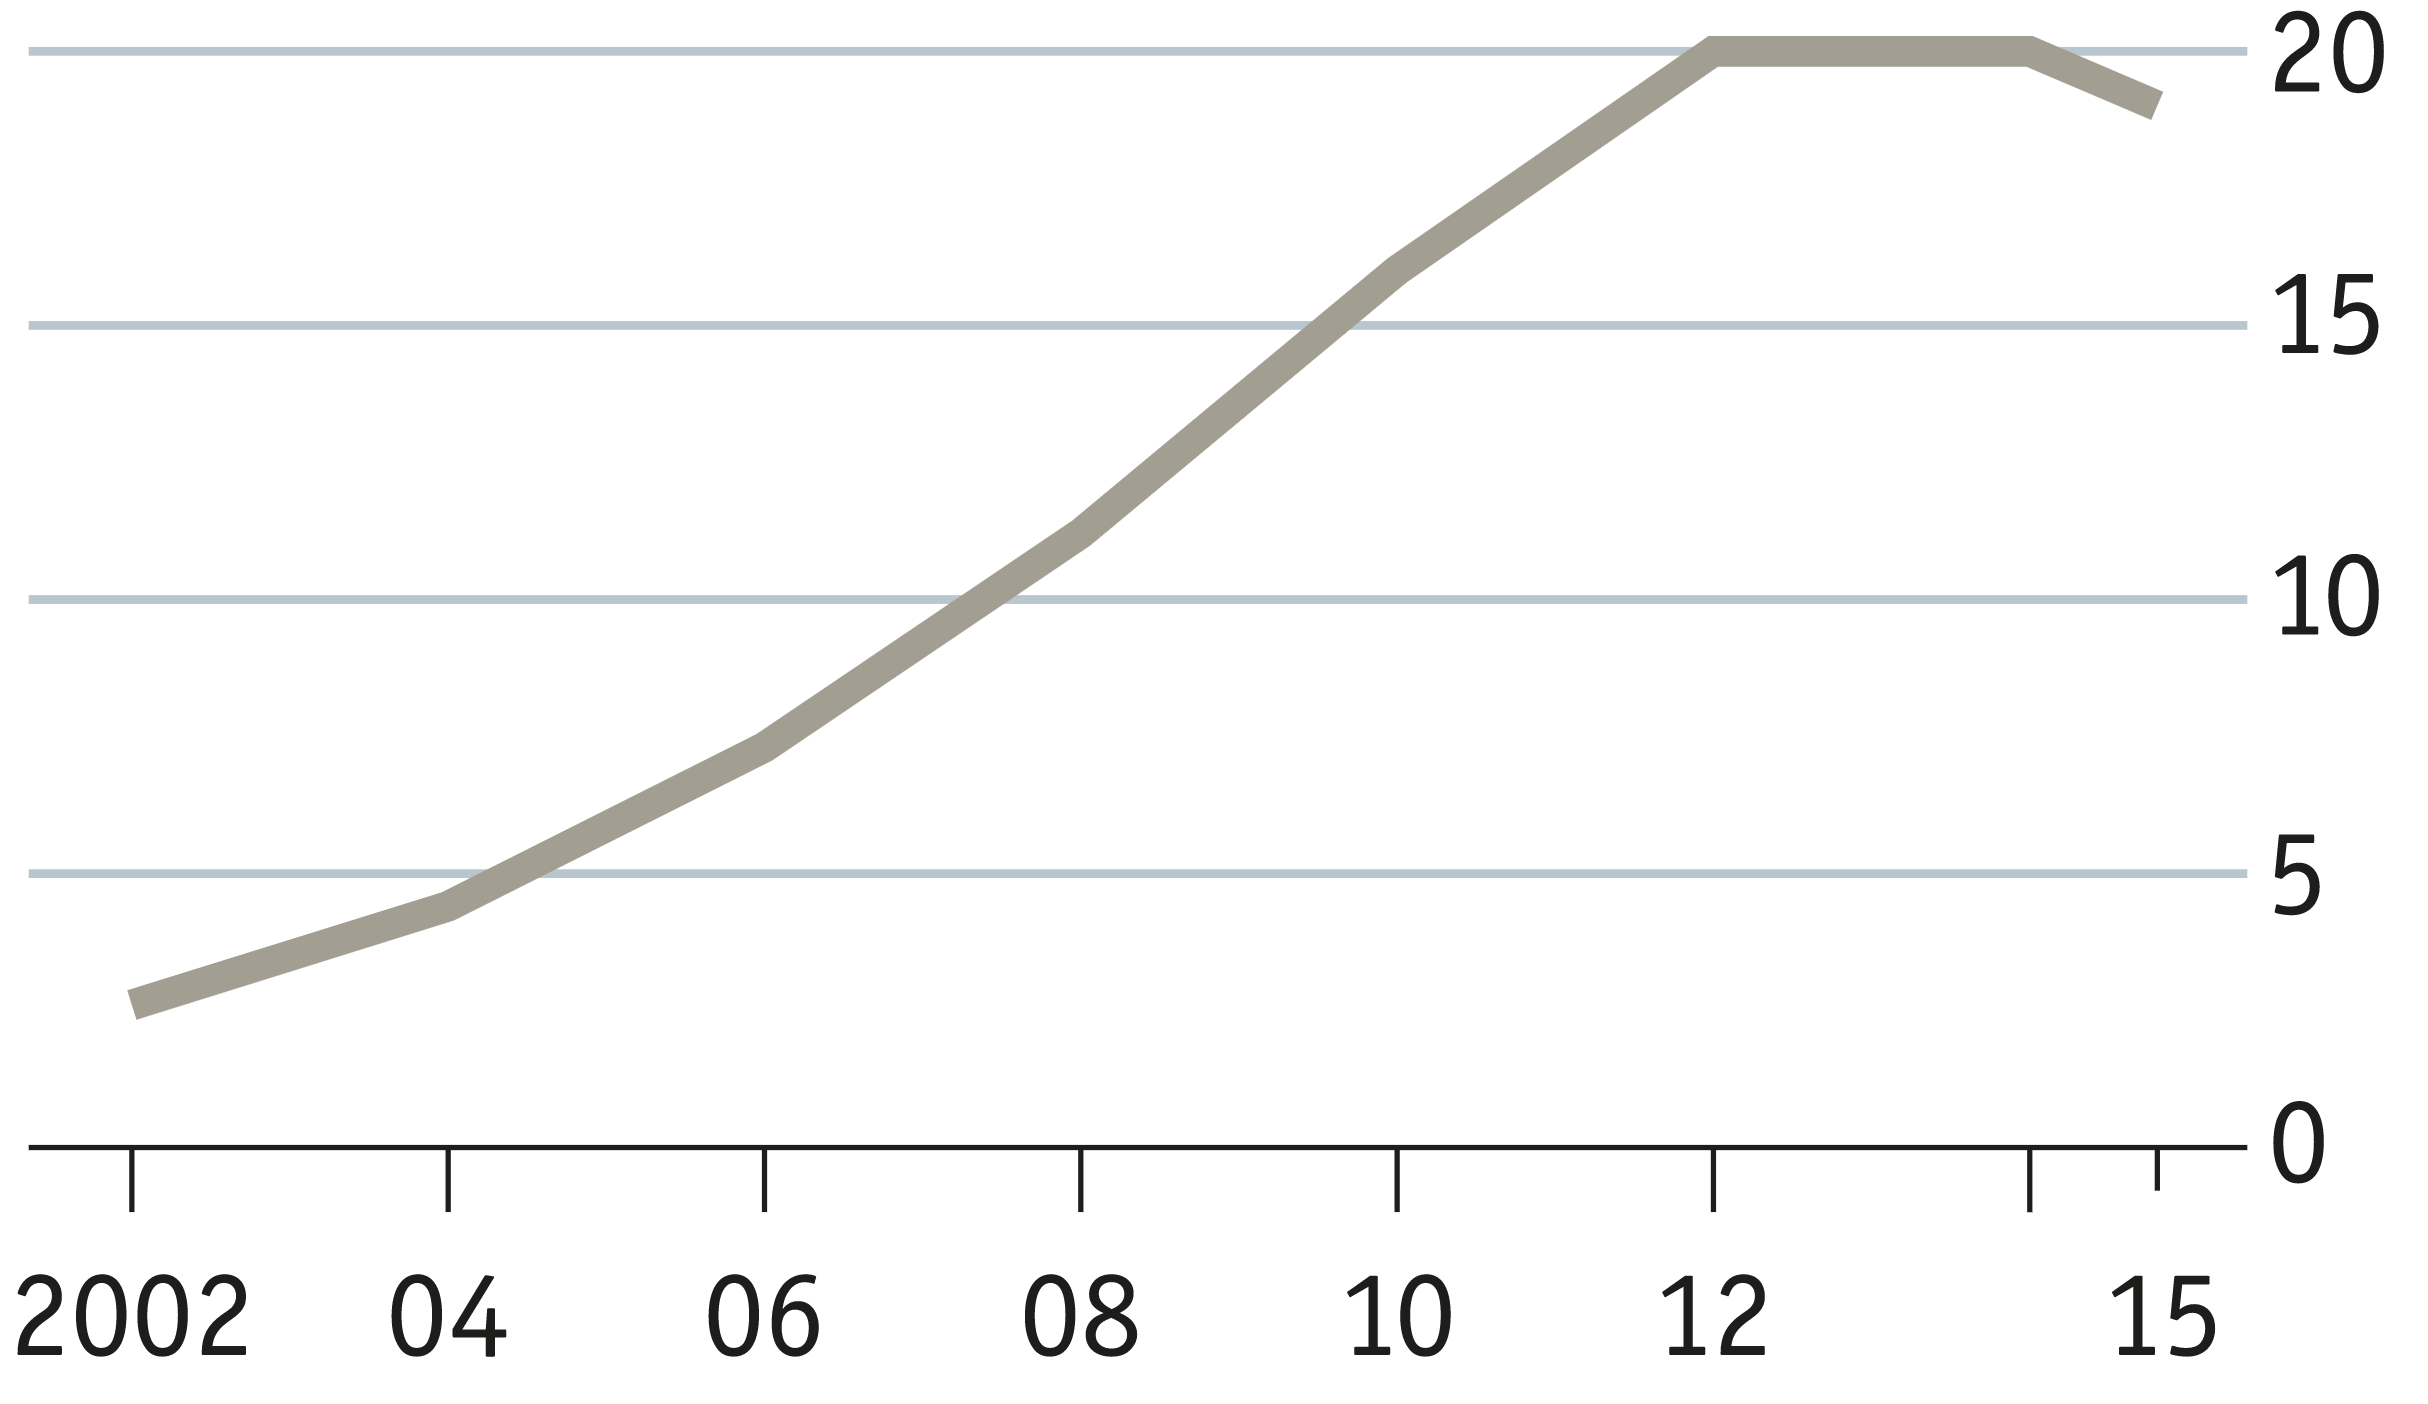
\includegraphics[width=8cm]{images/edl_moore_dollars.png}
        \caption{\label{fig:edl_moore_dollars} Nombre de transistors achetés par dollar dépensé\protect\footnotemark.}
        \end{figure}
        \footnotetext{Source: Intel ; rapport de presse ; Bob Colwell ; Linley Group; The Economist ; IB Consulting}

  %Data center
    

        Le prix d'un supercalculateur n'est pas seulement constitué de l'addition du prix des processeurs et des mémoires. Elle prend en compte le Coût Globale de Possession (TCO) (voir \autoref{sec:methodo_step4}). Cette valeur prend en compte le cumul des coûts du centre de données durant la totalité de son cycle de vie. Il tient compte du prix du bâtiment dans lequel se trouve le supercalculateur, de sa consommation électrique, mais aussi de l'opérationnel (personnel nécessaire pour sa gestion). Tous ces facteurs doivent être pris en compte, le prix de l'électricité tenant une grande part dans l'équation. 
        Pour les entreprises, le facteur économique est souvent le premier critère de décision. Les budgets alloués au développement et à l'utilisation d'une nouvelle plateforme sont décidés en amont et il est rare que des budgets supplémentaires soient alloués, même pour une plateforme plus performante. Lorsque HPE répond à des appels d'offres pour la construction d'un nouveau supercalculateur, les métriques utilisées sont les $FLOPS/\$$ ou $GB/s/\$$. Cette forte pression économique est une contrainte et il est difficile de proposer des sauts technologiques qui nécessitent de lourds investissements en amont sans connaître les retombés à l'avance. Lorsqu'une entreprise investit dans une solution, elle veut pouvoir quantifier à l'avance les bénéfices qu'elle peut en tirer. Lors de l'analyse du Top500, nous avons remarqué que la vitesse de l'accroissement des performances des supercalculateurs des entités avec les plus petits budgets avait ralenti 4 ans (2008) avant le reste du Top500 (2012). 
    
        
    \subsubsection{La consommation énergétique}\label{sec:edl_chal_energie}
    %%%%%%%%%%%%%%%%%%%%%%%%%%%%%%%%%%%%%%%%%%%%%%%%%%%%%%%%%%%%%%%%%%%%%%%%
    %%%%%%%%%%%%%%%%%%%%%%%%%%%%%%%%%%%%%%%%%%%%%%%%%%%%%%%%%%%%%%%%%%%%%%%%
  
        L'investissement dans un supercalculateur ne concerne pas seulement son acquisition. Un budget conséquent doit être alloué à l'alimentation du matériel, mais aussi du système de refroidissement. L’évolution de la consommation des processeurs a nécessité le développement de systèmes de refroidissement ultra-optimisés. Toute l’énergie étant transformée en chaleur, des techniques telles que le refroidissement à l’eau et l’immersion dans des bains d’huile sont régulièrement utilisés. Si on regarde la consommation électrique des clusters du Top500, on constate qu'en moyenne ils consomment 1,4 mégawatt et que les 5 qui consomment le plus sont au-delà de 12 mégawatts (voir graphique \ref{pic_top500_power}). En supposant que le prix de l'électricité coûte 1 dollar par watt par années, l'alimentation de ces architectures coûte alors annuellement des millions de dollars (20 millions de dollars pour le premier).
        
        En plus du coût financier, il est important de considérer l'impact écologique de la consommation électrique de ces plateformes. Une étude a été menée pour évaluer l’évolution de l’entraînement des principaux réseaux de neurones (AlexNet, AlphaGo, GoogleNet…) \cite{strubell-etal-2019-energy}. La quantité de calculs nécessaire pour l’entraînement d’un réseau a été multipliée par 300 000 en 7 ans. L’étude rapporte l’empreinte carbone de l’entraînement de ces réseaux. Le $CO_2$ émis lors de l'entraînement d’un réseau équivaut au $CO_2$ émis par un passager réalisant 300 allers-retours en avion entre New York et San Francisco ou encore à l’émission de cinq voitures américaines durant toute leur durée de vie.
                
                \begin{figure}
                    \center
                    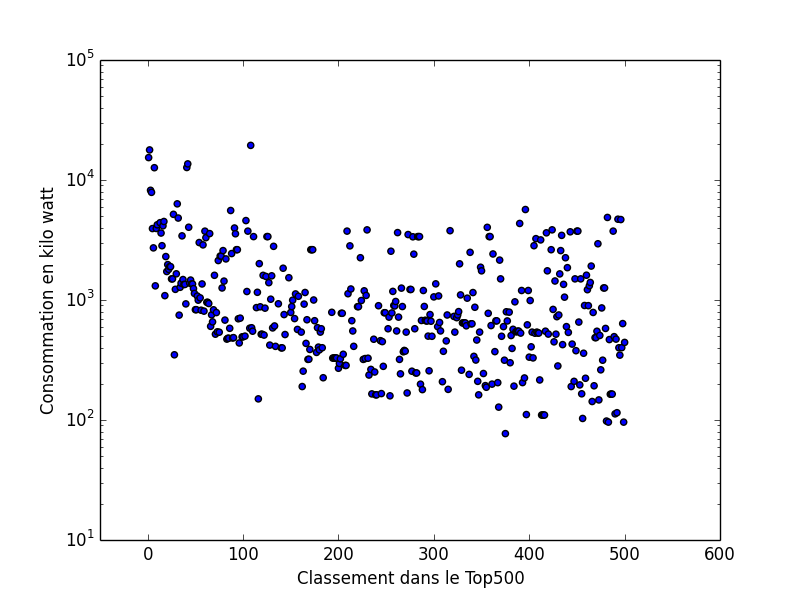
\includegraphics[width=10cm]{images/Chapitre1/pic_top500_power.png}
                    \caption{\label{pic_top500_power} Consommation électrique des 500 supercalculateurs les plus puissants (2018).}
                \end{figure}
      
      
        Le Département de l'énergie des États-Unis (DoE) a publié son rapport de propositions PathForward, et a établi qu'un supercalculateur exaflopique devra consommer au maximum entre 20 et 30 mégawatts \cite{Ang2016}. Actuellement, les quatre premiers supercalculateurs consomment entre 7 et 18 MW. La construction d'une plateforme exascale implique donc de réaliser 30 fois plus d'opérations avec une enveloppe énergétique seulement doublée. L'énergie est une contrainte majeure dans la construction d'une plateforme Exascale. Pour nous en rendre compte, nous étudions le dernier classement du Top500 paru en novembre 2019. Pour obtenir une puissance cumulée d'un exaFLOPS, il faut additionner la puissance des 105 premiers supercalculateurs du Top500. Une telle plateforme nécessiterait alors une alimentation de plusieurs centaines de mégawatts. Le même exercice peut être réalisé avec le classement du Green500 (voir \autoref{tab:green500}), qui classe les architectures les plus efficaces du Top500. Pour obtenir une puissance cumulée d'un exaFLOPS, il faudrait regrouper les 205 premiers supercalculateurs pour obtenir une plateforme consommant 279 MW. Ces rapides calculs permettent de montrer l'étendue vertigineuse des améliorations qui sont nécessaires pour la construction d'une plateforme qui respecterait les critères de consommation \cite{Ang2016}. 
        
        
        
        \paragraph{Consommation de la microarchitecture.} 
            
            Ajouter des serveurs pour la construction d'un supercalculateur plus puissant nécessite une plus grande puissance électrique. Cette technique est restée viable pendant plus de vingt ans, alors que les processeurs ne consommaient que quelques watts. Aujourd'hui, les processeurs utilisés ont une enveloppe thermique (TDP) dépassant la centaine de watts: 190 watts pour le processeur IBM Power9 22 coeurs (utilisé dans le supercalculateur Summit), 150 watts pour le processeur Intel Skylake 6148 20 coeurs (utilisé dans le 8e supercalculateur du classement du Top500 2019). Les plateformes les plus puissantes associent à un processeur un ou plusieurs accélérateurs (principalement des GPU). Chaque noeud du supercalculateur Summit possède ainsi 2 processeurs et 6 GPU NVidia V100 ayant chacun un TDP de 250 watts. À de telles consommations, il n'est plus viable d'ajouter des noeuds de calculs indéfiniment, que ce soit pour une raison de coût ou bien de faisabilité. En effet, les sites où sont construits les centres de données ont des lignes électriques déjà existantes et qui ne peuvent pas supporter de plus grandes puissances. Une partie des utilisateurs sont donc limités par cette enveloppe énergétique et doivent l'utiliser le plus efficacement pour la transformer en puissance de calcul. La consommation électrique des architectures varie fortement en fonction des opérations réalisées (voir \autoref{fig:energy_pj}). Que ce soit pour des architectures 32 bits \cite{Horowitz2014} ou 64 bits \cite{Leland2014} la consommation électrique des opérations élémentaires de la microarchitecture n’a que très peu évolué ces dernières années. Nous constatons que la majorité du budget énergétique est allouée au déplacement des données entre la mémoire et les caches. Il est donc primordial d'apporter des solutions matérielles et logicielles permettant de réduire la consommation de ces opérations.
        
            \begin{figure}
            \center
            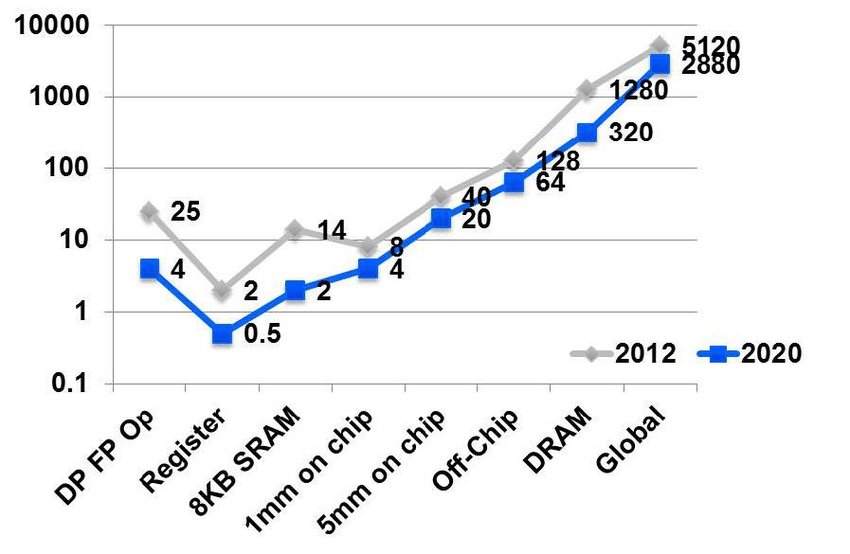
\includegraphics[width=10cm]{images/energy_pj.png}
            \caption{\label{fig:energy_pj} Coût énergétique, en picojoules (pJ) par opération à virgule flottante de 64 bits, pour diverses opérations courantes dans un ordinateur. La ligne supérieure (grise) représente le coût énergétique des opérations sur un processeur utilisé en 2012. La ligne inférieure (bleue) prévoit les coûts énergétiques en 2020 \cite{Leland2014}.}
            \end{figure}
            
                

        
        \paragraph{Le cas du supercalculateur Summit.} 
        
            Pour étudier la contrainte énergétique dans l'élaboration d'une plateforme Exascale, nous étudions certaines caractéristiques du supercalculateur Summit présentées dans le \autoref{tab:summit_analysis}. Ce dernier est classé numéro un au Top500 de novembre 2019 (voir \autoref{sec:Top500}). Il est aussi le premier supercalculateur du classement du Green500 consommant plus de 10 MW  (classé 5e en novembre 2019). Pour appréhender l'importance des efforts à fournir pour construire un supercalculateur capable d'exécuter $10^{18}$ opérations par seconde pour une application réelle, nous comparons l'efficacité énergétique de Summit avec celle d'un supercalculateur Exascale pour l'exécution du benchmark HPL.
        
            \begin{table}[]
            \centering
            \resizebox{\textwidth}{!}{%
            \begin{tabular}{|l|c|c|c|c|c|}
            \hline
            \rowcolor[HTML]{EFEFEF} 
            \textbf{Supercalculateur} & \textbf{\begin{tabular}[c]{@{}c@{}}Consommation\\ (MW)\end{tabular}} & \textbf{\begin{tabular}[c]{@{}c@{}}Perf. Linpack\\ (exaFLOPS)\end{tabular}} & \textbf{\begin{tabular}[c]{@{}c@{}}Efficacité énergétique\\ (GFLOP/watt)\end{tabular}} & \textbf{\begin{tabular}[c]{@{}c@{}}Budget énergétique\\ (pJ/opération)\end{tabular}} & \textbf{\begin{tabular}[c]{@{}c@{}}Conso. Linpack\\ (pJ/bit)\end{tabular}} \\ \hline
            \cellcolor[HTML]{EFEFEF}\textbf{Summit} & 10 & 0.200 & 20 & 50 & 0.25 \\ \hline
            \cellcolor[HTML]{EFEFEF}\textbf{Projet Exascale} & 20 - 30 & 1 & 50 - 33 & 20 - 30 & 0.1 - 0.15 \\ \hline
            \end{tabular}%
            }
            \caption{Comparaison de l'efficacité énergétique du supercalculateur Summit et de l'efficacité théorique d'une plateforme exascale\textbackslash{}cite\{Bergman2018\}.}
            \label{tab:summit_analysis}
            \end{table}
    
    
            Pour fonctionner, Summit a besoin d'une puissance de 10 MW. En novembre 2019, il a atteint une performance de 200 pétaFLOPS ($10^{15}$ \gls{FLOPS}) lors de l'exécution du benchmark Linpack. Son efficacité énergétique est donc de 20 GFLOP/watt. Un supercalculateur exaflopique consommant entre 20 et 30 MW aurait quant à lui, une efficacité énergétique comprise entre 33 et 50 GFLOP/watt. Le challenge est donc de construire une plateforme 5 fois plus puissante tout en étant deux fois plus efficace énergétiquement. Cependant, le défaut du benchmark Linpack est qu'il ne reflète pas le comportement des applications industrielles. En effet, contrairement aux applications réelles, il ne nécessite aucune communication entre les noeuds, et les instructions sont réalisées sur des données présentes dans le cache. Atteindre un exaFLOPS sur le benchmark HPL sera bien plus facile que d'atteindre la même performance avec une application réelle dont la consommation est principalement due aux déplacements mémoires. Pour mieux appréhender l'impact énergétique des déplacements mémoires, nous calculons l'efficacité énergétique des deux supercalculateurs étudiés en joule/FLOP:
            \begin{equation}
                 \frac{FLOPS}{watt}  =  \frac{\frac{FLOP}{seconde}}  { \frac{joule}{second}} =  \frac{FLOP}{joule}
            \end{equation}
            Nous calculons ainsi le \textit{budget} disponible pour exécuter une opération flottante: 50 pJ pour Summit, contre 20 pJ et 30 pJ pour le supercalculateur Exascale. En moyenne, l'application exécute des instructions vectorielles de 200 bits \footnote{Source - \url{https://insidehpc.com/2019/07/flexibly-scalable-high-performance-architectures-with-embedded-photonics/}}. L'énergie dépensée par Summit pour calculer un bit est alors de 0.25 pJ. Pour une plateforme exascale, ce budget énergétique serait alors compris en 0.1 et 0.15 pJ/bit.
            
            Un accès à la mémoire se compte en centaine de picojoules par bit et en millier lorsqu'il s'agit de communication entre deux noeuds de calculs. Lorsque l'énergie disponible est de 0.1 pJ/bit et qu'un accès mémoire peut dépasser de cent fois ce budget, il est facile de comprendre que l'essentiel des innovations doivent se porter sur l'amélioration des communications (à l'intérieur des serveurs, mais aussi à l'extérieur) que ce soit par l'utilisation de nouvelles technologies ou d'une restructuration des microarchitectures. Les applications et les algorithmes doivent eux optimiser l'utilisation des données locales pour tirer profit des principes de localité (voir \autoref{sec:locality}).


    \subsubsection{La complexité}\label{sec:edl_chal_complexite}
    %%%%%%%%%%%%%%%%%%%%%%%%%%%%%%%%%%%%%%%%%%%%%%%%%%%%%%%%%%%%%%%%%%%%%%%%
    %%%%%%%%%%%%%%%%%%%%%%%%%%%%%%%%%%%%%%%%%%%%%%%%%%%%%%%%%%%%%%%%%%%%%%%%
        
        Comme présenté dans l'\aref{chap:sota:materiel}, les architectures des ordinateurs ont reçu de nombreuses améliorations au fil des ans. Ces améliorations se sont additionnées et ont permit le développement des processeurs tels que nous les connaissons aujourd'hui: une hiérarchie mémoire, plusieurs coeurs (logique et physique), un pipeline comportant souvent plus de dix étapes, des systèmes d'exécution dans le désordre ou encore de préchargement mémoire. 
        
        La complexification est aussi présente dans le logiciel. Pour tirer parti des fonctionnalités offertes par le matériel, plusieurs modèles de programmation sont utilisés pour par exemple exploiter la mémoire partagée et distribuée ou utiliser les différents coeurs d'un processeur. En fonction des tâches à réaliser, plusieurs langages peuvent être utilisés dans une même application (C, C++, fortran, python, cuda...). La programmation \textbf{efficace} d'un supercalculateur est ainsi devenue une tâche très difficile. La complexification du matériel et du logiciel a un fort impact sur la performance des applications qui parviennent rarement à exploiter une part significative de la performance disponible. La performance d’une même application peut fortement varier à cause d’une subtilité (la configuration du BIOS, un réglage du système d’exploitation). Certaines technologies (FPGA, GPU) ne sont pas envisagées par des entreprises, car l'adaptation de leurs applications pour fonctionner sur celles-ci est très difficile. Pour s'extraire de la complexité grandissante des plateformes HPC et de leur gestion, de plus en plus d'utilisateurs se tournent vers des solutions dématérialisées telles que le \textit{cloud}.
        
        %Dans le classement du Top500, on remarque ainsi que les supercalculateurs atteignent rarement plus de 80\% d'efficacité sur une application simple comme Linpack\cite{Dongarra2003}. Pour des applications réelles, cette efficacité est encore plus faible, parfois inférieure à 10\%\cite{Oliker2005}. 
        %La complexité des architectures a aussi un impact sur l'efficacité énergétique des plateformes, par exemple le mécanisme de prédiction de branchement ou l'agrandissement des différents niveaux du \textit{pipeline} (voir \autoref{sec:pipeline}).
        
        \paragraph{La sécurité.} La complexité du matériel et des couches logicielles représente un grand risque d'exploitation de faille de sécurité. Les applications utilisent de nombreuses librairies qui peuvent présenter des failles, et la difficulté de les mettre à jour (pour la stabilité des applications) peut permettre aux attaquants d'exploiter ces failles. L'accumulation de fonctionnalités a aussi rendu ces architectures sujettes à différentes attaques. En 2018, les chercheurs de Google \cite{kocher2018spectre} ont découvert une faille majeure dans le prédicteur de branchement des processeurs Intel (voir \autoref{sec:micro}). Aujourd'hui, les supercalculateurs sont rarement directement connectés au réseau internet, rendant difficile l'attaque de ces plateformes. Cependant, la vision exascale présentée dans le début du chapitre implique la collecte de données et le traitement des données au plus proche de la source de leur création ainsi que l'acheminement de certains résultats vers les centres de calculs, exposant de nombreux lieux d'attaque. Il n’est pas envisageable d'utiliser des voitures autonomes possédant des processeurs, des mémoires, des dizaines de couches logiciels pouvant être attaqués. De même, les données personnelles, tels que les données médicales enregistrées par les montres connectées sont très sensibles.
    
        
        \paragraph{Passage à l'échelle.} Pour obtenir un supercalculateur exascale, il est techniquement possible de construire 5 supercalculateurs de la puissance du Summit et d’agréger leur performance. Cependant, pour les raisons de coût, principalement lié à la consommation énergétique, cette solution n’est pas envisageable. À une telle échelle, le nombre de serveurs serait si important (supérieur à 30000) que des problèmes insoupçonnés à des tailles moindres feraient leur apparition. Les pannes des matériels, les congestions de réseaux et la capacité des applications à utiliser un grand nombre de serveurs impacteraient leur performance rendant le supercalculateur très inefficace. En effet, la programmation parallèle nécessite la synchronisation des ressources à différentes étapes du calculs pour partager des résultats intermédiaires. Ainsi, les pannes matériel d'une seule ressource de calcul ont de forts impacts sur la performance des applications de calculs parallèles. 
        %Ces infrastructures seront utilisées pour exécuter des applications pendant plusieurs heures ou mêmes jours. Il est donc nécessaire de développer des systèmes de reprises suite à une erreur sans avoir à tout recommencer \cite{farjallah2014preparing} grâce à des mécanismes de point de contrôle (\textit{checkpoint}) \cite{Zheng2012}
        

    \subsubsection{Les nouvelles technologies}\label{sec:edl_chal_new_techno}
    %%%%%%%%%%%%%%%%%%%%%%%%%%%%%%%%%%%%%%%%%%%%%%%%%%%%%%%%%%%%%%%%%%%%%%%%    %%%%%%%%%%%%%%%%%%%%%%%%%%%%%%%%%%%%%%%%%%%%%%%%%%%%%%%%%%%%%%%%%%%%%%%%

        Nous avons montré précédemment que les utilisateurs étaient en demande de puissance de calcul supplémentaires. 
        Le classement du Top500,  réalisé tous les 6 mois, permet de classer les plateformes les plus récentes. Les nombreux supercalculateurs construits chaque année rentrent au classement, remplaçant les anciennes plateformes moins performantes. Sur la \autoref{fig:edl_top500_age}, nous constatons que l'âge moyen du Top500 a doublé en quelques années indiquant la difficulté à produire des supercalculateurs plus performantes. Alors que l'âge moyen du classement oscillait autour de 7 mois pour les 23 premières années du classement, il a dépassé les 15 mois depuis les années 2013. Ces deux constats montrent que les utilisateurs de HPC ne renouvellent plus leurs supercalculateurs, car ils ne trouvent plus de solutions matérielles suffisamment intéressantes pour motiver de nouveaux investissements. De nouvelles technologies doivent émerger pour obtenir de réels gains de performance. L'histoire récente nous a prouvé que ce chemin était le bon à suivre avec l'utilisation des GPU (ou d'accélérateurs dédiés comme les TPU de Google) pour accélérer les applications d'apprentissage par machine. Les pressions économique et énergétique présentées précédemment nous indiquent que de nombreuses avancées doivent être réalisées dans tous les domaines touchant au HPC: les processeurs, les accélérateurs, les mémoires, les réseaux ou bien la partie logiciel. 
        
        
                  
            \begin{figure}
                \center
                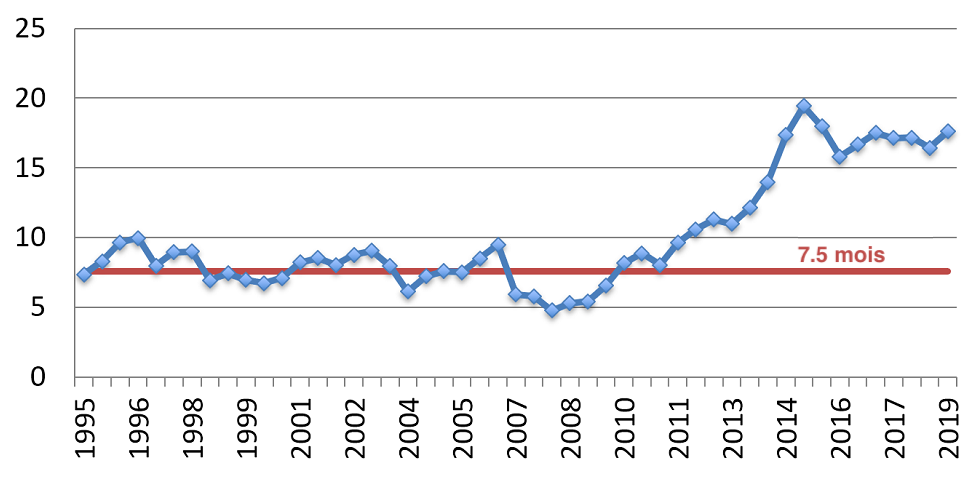
\includegraphics[width=10cm]{images/edl_top500_age.png}
                \caption{\label{fig:edl_top500_age} Âge moyen des supercalculateurs classés au Top500 \cite{Strohmaier2018}.}
            \end{figure}
       
        %Exemple de nouveauté
        

        \paragraph[Explosion cambrienne] {Explosion ``cambrienne'' \footnote{L’explosion cambrienne désigne l'apparition soudaine (à l'échelle des temps géologiques) de la plupart des grands embranchements actuels des animaux pluricellulaires ainsi qu'une grande diversification des espèces animales, végétales et bactériennes (wikipédia).}}
        
            De nouvelles technologies existent ou sont en cours de développement. Dans la \autoref{sec:oppo_new_tech}, nous montrons que de nombreuses solutions matérielles, technologiques et logiciels peuvent être utilisées. Des accélérateurs et des mémoires très spécifiques pourront être utilisés. Les utilisateurs de HPC et les architectes doivent alors connaître les besoins de leurs applications pour choisir quelles technologies utiliser (type et quantité de mémoire, utilisation d'accélérateurs). Si ces nouvelles technologies peuvent être une réelle opportunité pour l'élaboration de plateformes plus puissantes et plus efficaces, elles sont aussi un challenge. En effet, jusqu’à récemment, la majorité des plateformes étaient construites de façon similaire: un processeur x86 pouvant être associé à un GPU (voir \autoref{sec:edl_hpc_hetero}). Si les applications obtenaient de faibles performances, il était difficile de s'orienter vers d'autres solutions alors inexistantes. La majorité des supercalculateurs sont utilisés par différents utilisateurs et exécutent différents types d'applications. Le choix des technologies utilisées doit alors prendre en compte ces différentes applications pour construire la plateforme la plus efficace possible. Souvent ces centres de calculs seront hétérogènes avec différents processeurs.
        
        \paragraph{Nouveautés au Top500.} En étudiant le classement du Top500, nous constatons les premiers signes de l'évolution des plateformes qui utilisent de nouveaux types de processeurs ou d'accélérateurs (voir \autoref{fig:new_proc}). En novembre 2019, trois supercalculateurs classés à la 84e, 72e et 116e place étaient équipés de processeur Sparc64 XIfx \cite{Yoshida2018}. Ce processeur est produit par Fujitsu et possède 34 coeurs (dont deux réservés en priorité au système d'exploitation et à la gestion des communications). Il possède 24 Mb de cache L2 et atteint une performance de 1,1 téraFLOPS (voir \autoref{fig:edl_sparc64}). Pour atteindre de hautes performances sur des applications réelles, le processeur est doté d'une mémoire empilée HMC de 32 GB \cite{Garg2017}. Concernant les accélérateurs, nous pouvons citer le coprocesseur Matrix-2000 qui a permis de doubler la puissance du supercalculateur chinois Tianhe-2 en remplaçant les anciens accélérateurs KNL par une nouvelle architecture développée exclusivement pour lui. Cet accélérateur 64 bits produit par NUDT, possède 128 coeurs RISC à 1,2 GHz permettant d'atteindre une performance crête de 4,92 téraFLOPS pour une enveloppe thermique de 240W. Quatre groupes de 32 coeurs sont reliés à la mémoire avec un total de 8 canaux mémoires (voir \autoref{fig:edlp_matrix_2000}). 
        
          
        \begin{figure}[t!]
            \centering
            \begin{subfigure}[t]{0.48\textwidth}
                \centering
                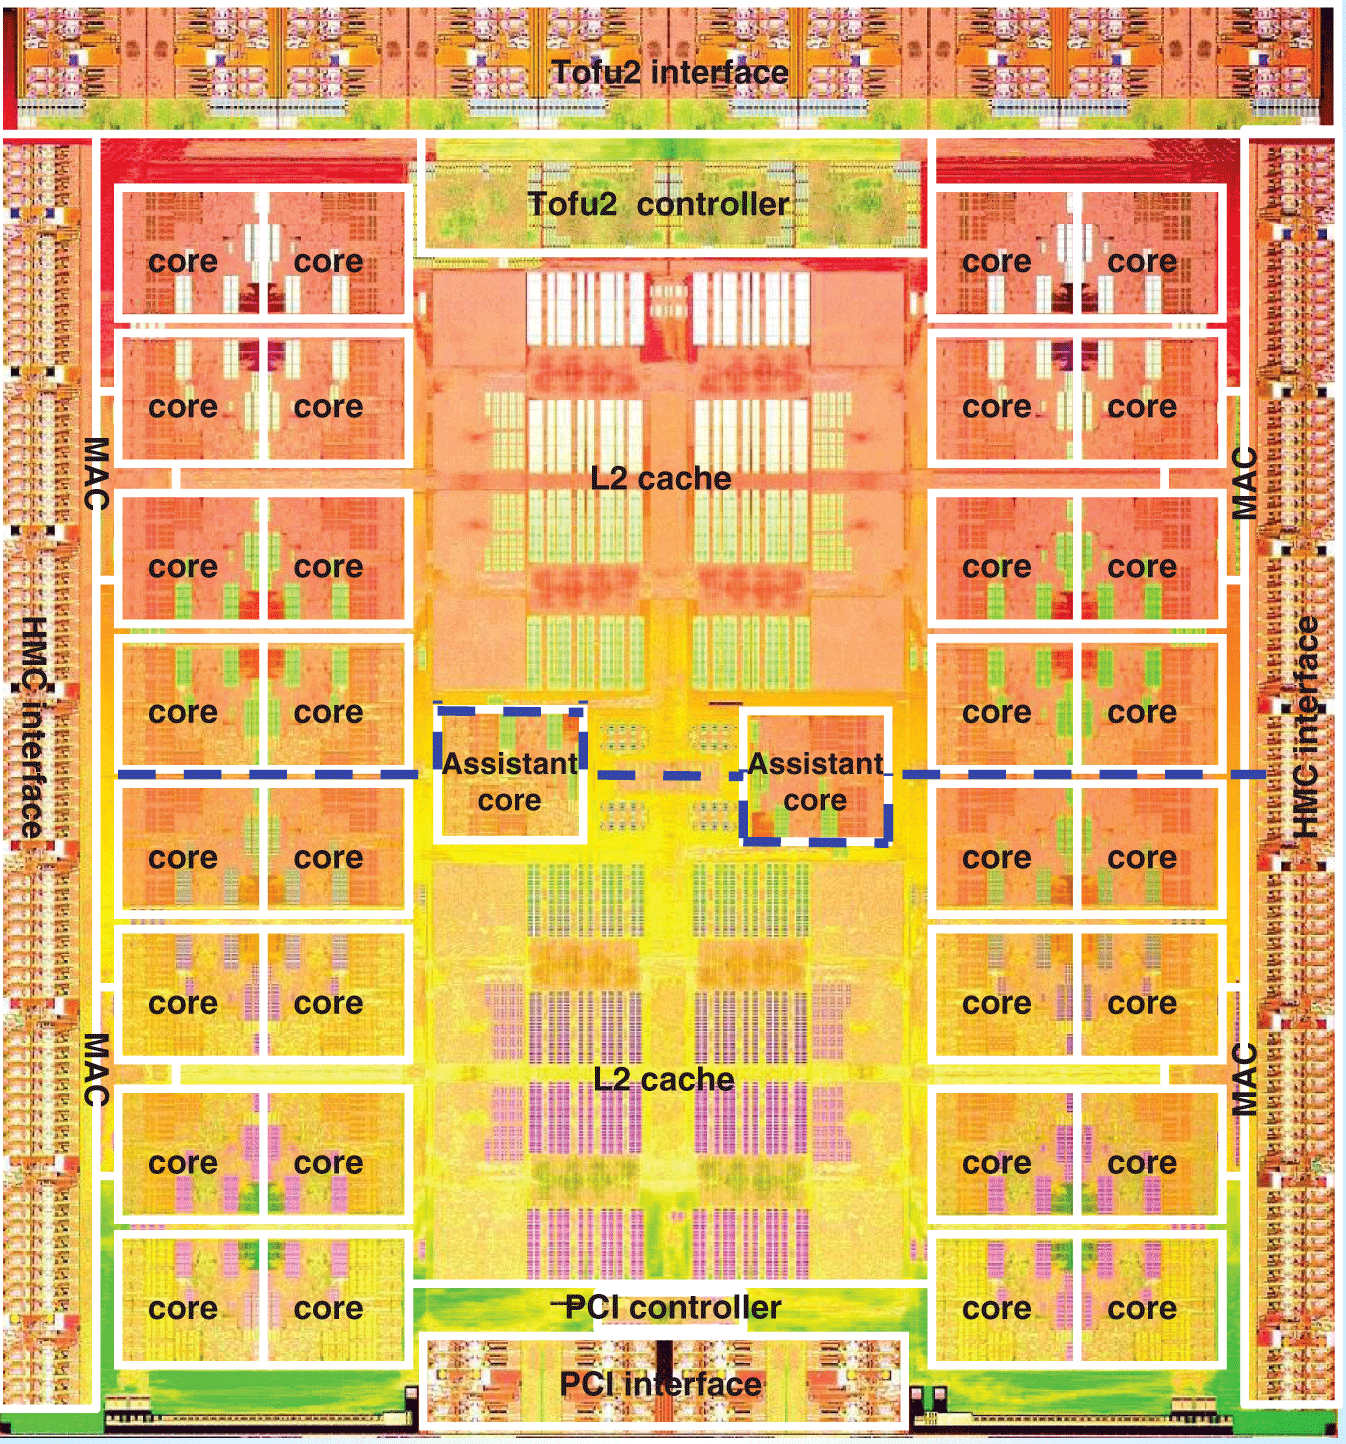
\includegraphics[width=0.9\linewidth]{images/edl_sparc64.png}
                \caption{\label{fig:edl_sparc64} Le processeur Sparc64 est produit par Fujitsu et utilise une mémoire empilée HMC\cite{7021857}.}
            \end{subfigure}\hfill
            \begin{subfigure}[t]{0.48\textwidth}
                \centering
                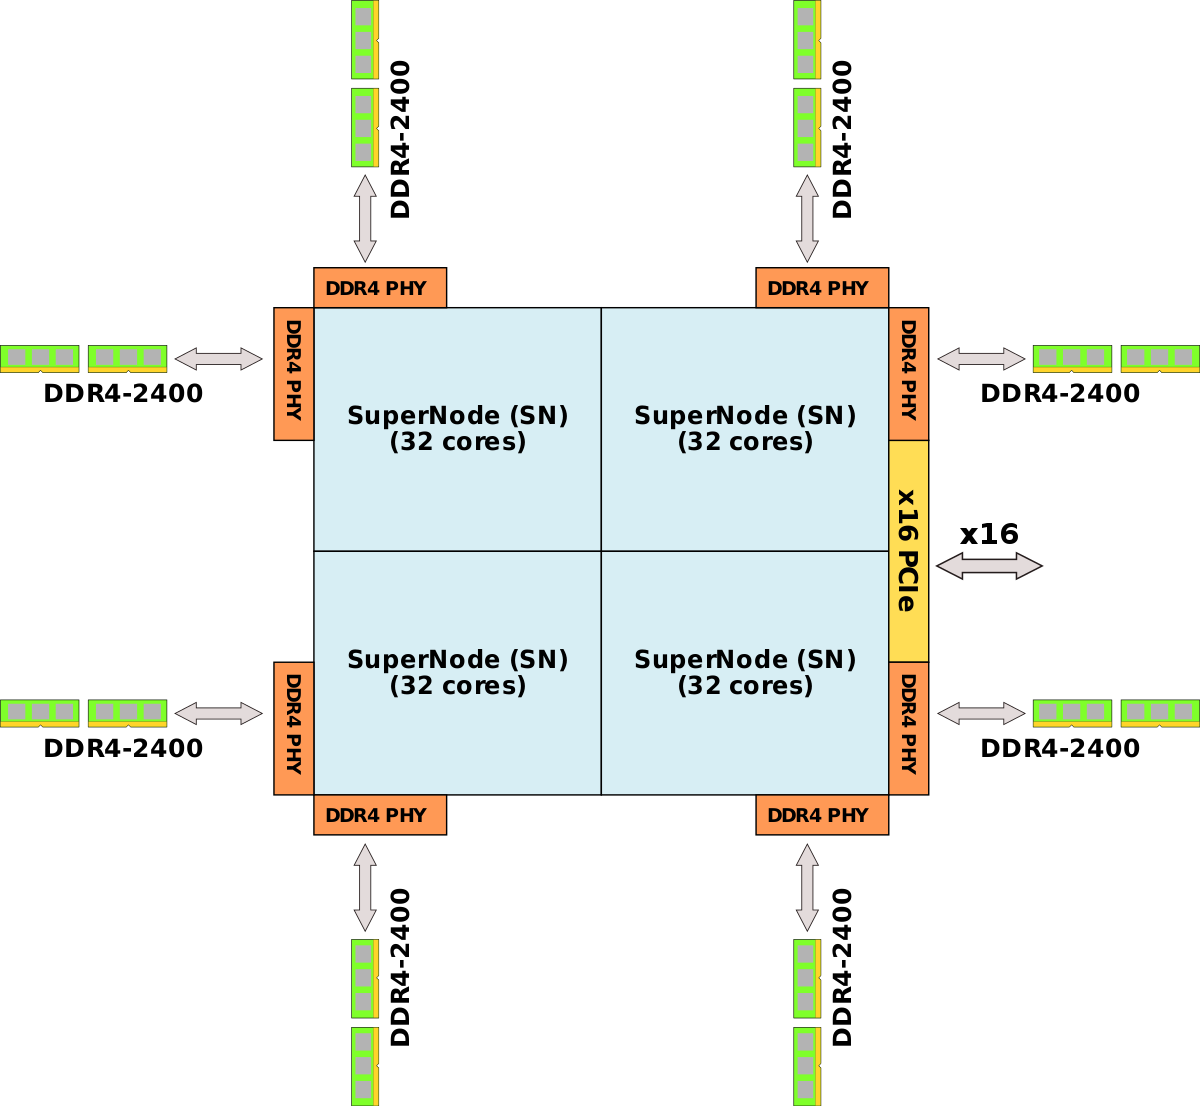
\includegraphics[width=\linewidth]{images/edlp_matrix_2000.png}
                \caption{\label{fig:edlp_matrix_2000}Le coprocesseur Matrix 2000 possède 128 coeurs et 8 canaux mémoires.}
            \end{subfigure}
            \caption{\label{fig:new_proc} De nouvelles architectures sont utilisées dans les supercalculateurs classés au Top500.}
        \end{figure}

           
    \subsubsection{Rapidité de l'évaluation des nouvelles technologies} \label{sec:edl_chal_vitesse}
    %%%%%%%%%%%%%%%%%%%%%%%%%%%%%%%%%%%%%%%%%%%%%%%%%%%%%%%%%%%%%%%%%%%%%%%%    %%%%%%%%%%%%%%%%%%%%%%%%%%%%%%%%%%%%%%%%%%%%%%%%%%%%%%%%%%%%%%%%%%%%%%%%
        
        Face à l'arrivée de ces nombreuses technologies, les entreprises doivent rapidement être capables d'évaluer leurs qualités et leurs défauts et quantifier leur adéquation avec leurs applications. Les évolutions récentes sont très rapides avec le développement de dizaines de modèles de mémoire, de nouveaux accélérateurs et de processeurs. Certaines technologies encore en développement sont déjà dépassées par l’annonce de nouvelles technologies.
        
        Une technologie émergente, très performante pour une application, avec des consommations énergétiques ou un coût très faible peut permettre à une industrie de faire un bond de performances dans un domaine. Grâce à ces technologies, l'économie d'un domaine peut être fortement modifiée en permettant de réaliser des simulations dix fois plus rapidement ou en divisant leur coût du même facteur.
                
        La vitesse de décision et d'utilisation d'une nouvelle technologie dans notre société mondialisée est cruciale. Les entreprises doivent donc disposer de moyens (technique et financier) pour se tenir à l'état de l'art des technologies. Le développement de partenariat (avec des universités par exemple) est une des clefs permettant de s’assurer de la capacité des entreprises à ingérer ces nouvelles technologies.


    \subsubsection{L'expertise}\label{sec:edl_chal_expertise}
    %%%%%%%%%%%%%%%%%%%%%%%%%%%%%%%%%%%%%%%%%%%%%%%%%%%%%%%%%%%%%%%%%%%%%%%
    %%%%%%%%%%%%%%%%%%%%%%%%%%%%%%%%%%%%%%%%%%%%%%%%%%%%%%%%%%%%%%%%%%%%%%%%

        Pour construire les plateformes de demain, il est nécessaire de pouvoir qualifier les nouvelles architectures émergentes. Cette qualification devant se faire rapidement sur des dizaines d'architectures différentes, il est important pour les acteurs du HPC d'avoir les moyens adéquats pour réaliser cette mission. Pour motiver les choix réalisés, une modélisation économique des performances ($FLOP/\$$, $GB/s/\$$) doit pouvoir être réalisée. Une fois les architectures sélectionnées, les programmeurs doivent être capables d'extraire une part importante des performances disponibles. Les architectures ciblées pouvant être très différentes des processeurs x86 largement utilisés aujourd'hui, les programmeurs doivent avoir de solides connaissances et les outils adaptés, sans quoi certaines architectures devront être abandonnées. Les outils à leur disposition doivent leur permettre d'établir un profil des besoins de son application pour pouvoir caractériser et sélectionner les différentes plateformes. Pour étudier son application et valider leur performance une fois le code porté, il est nécessaire d'avoir des outils facilement utilisables sur différentes plateformes (et différentes microarchitectures).
        
        Les FPGA (Field Programmable Gate Array) en sont un bon exemple. Cette technologie permet de faire des périphériques très performants et très efficaces en termes de consommation électrique. L'idée principale étant de laisser au programmeur le développement complet du circuit électronique pour qu'il corresponde parfaitement à son besoin. Mais la programmation de tels circuits est très complexe et demande des mois, souvent des années pour des codes industriels, pour être réalisée. Ainsi, malgré l'efficacité, prouvée, de cette technologie, les entreprises ne s'y lancent pas à cause des coûts engendrés par l'achat du matériel et la taille des équipes requises pour programmer et supporter les applications. 
        
        
        %\paragraph{Programmation des supercalculateurs.} Dans la \autoref{sec:edl_chal_complexite} nous avons rappelé la complexité de programmer un supercalculateur, qui nécessite l'utilisation de plusieurs modèles de programmation et souvent de plusieurs langages. L'apparition de plateforme hétérogène (voir \autoref{sec:edl_hpc_hetero}) va rendre la tâche d'autant plus difficile. Pour l'aider, le programmeur doit avoir à sa disposition une couche logicielle et un modèle de programmation pour l’aider, lui permettant de se concentrer seulement sur le développement de son algorithme. Les outils de répartition de charges doivent être améliorés pour prendre en compte l'hétérogénéité des architectures disponible.
        
        
        \paragraph{Optimisations des codes.} 
            
            Le challenge de l’exascale ne vient pas seulement du matériel et des technologies que nous allons utiliser comme le soulignent certains travaux \cite{barrett2012navigating}. Il  nécessite aussi de repenser une grande partie des logiciels. Cette partie est très délicate, car les applications atteignent souvent plusieurs dizaines de milliers de lignes de codes. Changer un compilateur ou un debugger peut alors s’avérer plus complexe qu'il n’y parait. Pour atteindre les meilleures performances possible, les programmeurs doivent être capables d'écrire des applications optimisées pour les architectures utilisées. Pour cela, il est nécessaire de restructurer le code ou d'utiliser d'autres algorithmes pour tirer parti des caractéristiques du matériel (hiérarchie de cache, taille de la mémoire, nombre de coeurs...). Des optimisations telles que le découpage en bloc \cite{Xue2012} ou le \textit{time squewing} \cite{Wonnacott2002} existent et ont prouvé leur efficacité. Cependant, leur implémentation sur des applications industrielles peut être très fastidieuse et les performances atteintes peuvent être différentes de celles attendues. 
            
            %Cette partie pourrait être laissée au compilateur, mais il est très difficile de proposer un tel compilateur générique étant capable de les implémenter. Les compilateurs ont un rôle central dans le développement et l’exécution des applications, car ils sont l’intermédiaire entre le programmeur et le matériel. Leur efficacité à générer du code de qualité est primordiale pour tirer le maximum de performances de ces architectures complexes.

        %Algo
        \paragraph{Adapter les algorithmes.} Une source (presque) inépuisable d'accélération des applications vient de l'utilisation de nouveaux algorithmes. La \autoref{fig:edl_new_algo}, montre comment l'utilisation de nouvelles méthodes mathématiques permet d'accélérer de plusieurs facteurs la résolution d'une équation de poisson. Une application nécessitant 6 mois de calculs en 1947 peut être résolue grâce à une méthode multi grille \cite{Brandt1982} en moins d'une seconde.
            
            Pour réduire le nombre d’opérations lors de la multiplication de matrices pour les algorithmes d’apprentissage par machine, plusieurs techniques peuvent être utilisées \cite{Sze2017}: la transformée de Fourier rapide \cite{Vasilache2014}, l’algorithme de Strassen \cite{Cong2014} ou encore l'algorithme de Coppersmith-Winograd \cite{Li2016}. En fonction des caractéristiques de l’architecture (stockage disponible), du besoin de stabilité numérique, ou de la taille des matrices utilisées, chaque méthode à ses avantages et inconvénients. Le compilateur peut alors choisir la meilleure technique à utiliser en fonction de ces paramètres.
    
            \begin{figure}
            \center
            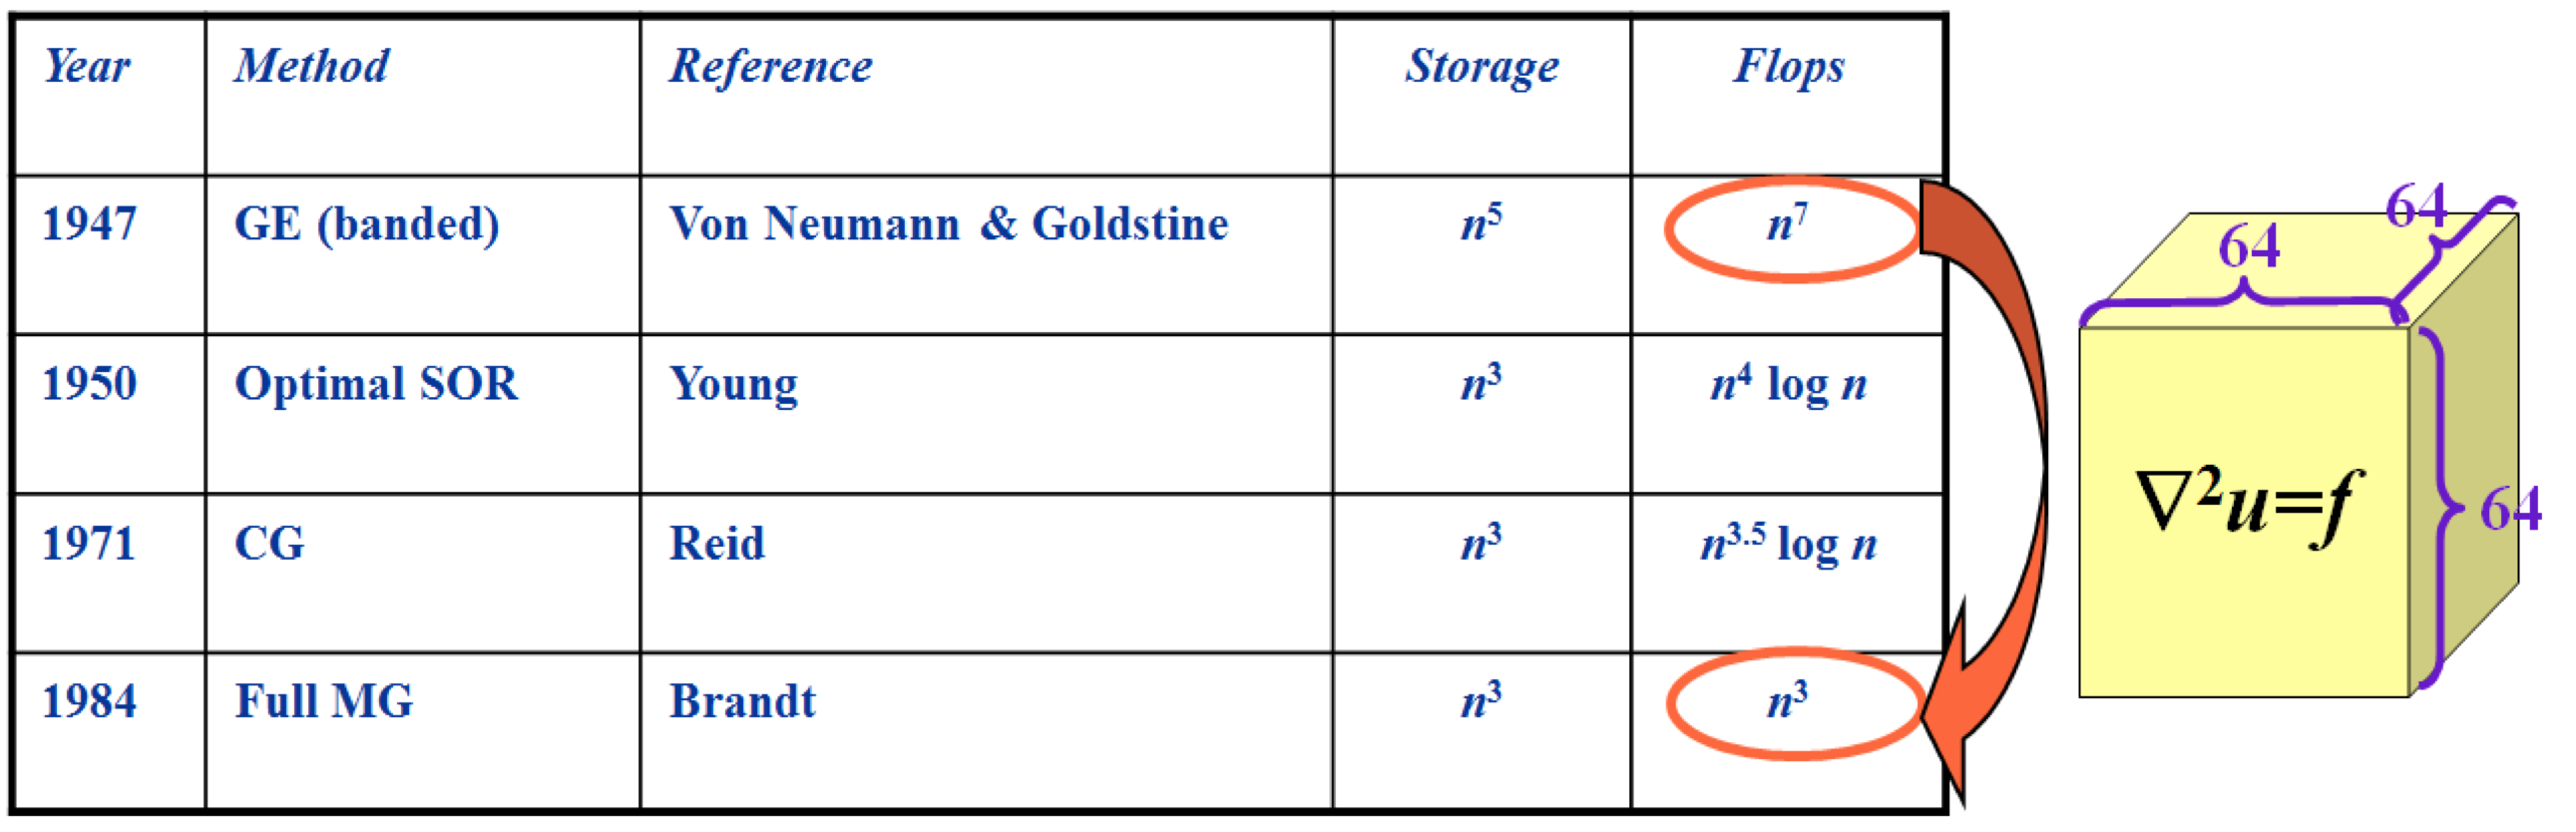
\includegraphics[width=14cm]{images/edl_new_algo.png}
            \caption{\label{fig:edl_new_algo} L'utilisation de nouvelle méthodes mathématique à permis de réduire de plusieurs facteurs la quantité de stockage (\textit{storage}) et le nombre de calculs nécessaires (\textit{flops}) pour la résolution d'une équation de poisson\protect\footnotemark.}
            \end{figure}
            \footnotetext{Tableau extrait de la présentation de David Keyes - \url{http://www.cs.odu.edu/~keyes/talks/SC_IMI.ppt}}

            Pour les plateformes exascale, les algorithmes doivent être adaptés à certaines contraintes. Le coût des déplacements des données, en énergie et en temps, doit être le moteur de leur développement et de leurs améliorations. En effet, le coût énergétique de l'exécution d’une opération flottante peut être considéré comme gratuit quand on le compare au coût du déplacement des données. La plus grande pénalité venant des communications entre les noeuds de calculs, les algorithmes doivent réduire au maximum ces communications en découpant stratégiquement le jeu de données. Il peut même être avantageux de recalculer certains résultats localement, plutôt que de les communiquer entre deux serveurs. L'algorithme de Strassen \cite{Lipshitz2012} permet par exemple la multiplication de deux matrices sans échanges de données. Ces techniques ont un gain double: elles sont plus rapides, car l’exécution n’est pas pénalisée par la performance du réseau, et elles sont plus efficaces énergétiquement, car elles ne payent pas le coût de la communication des données. Cependant, ces méthodes peuvent entraîner des problèmes de stabilité numérique \cite{khabou2013dense}. 
                        

        \paragraph{Challenge.}  
        
            La complexification des applications et du matériel confronté au manque de connaissances et d'outils des utilisateurs se traduit par une mauvaise utilisation des plateformes évoquée dans la \autoref{sec:Top500}. Bien que la recherche ait réalisé de nombreuses découvertes, peu d'entre elles sont réellement appliquées sur les codes industriels. La loi de Moore assurant une évolution constante des performances des architectures, l’analyse et l’optimisation des codes ont été laissées de côté. Les investissements réalisés dans le développement des matériels se sont faits au détriment des logiciels. Aujourd'hui, nous constatons un manque de connaissances fines des architectures dû à leur complexité croissante ainsi que le manque d'outils adéquats pour réaliser les optimisations nécessaires.
        

\section{Opportunités}\label{sec:oppo}
%%%%%%%%%%%%%%%%%%%%%%%%%%%%%%%%%%%%%%%%%%%%%%%%%%%%%%%%%%%%%%%%%%%%%%%%
    
    %Fin d'un modèle
    Nous avons montré dans les sections précédentes que poursuivre la stratégie qui consistait à ajouter toujours plus de serveurs pour construire un supercalculateur, n'est plus viable. Nous avons présenté les principaux défis que les utilisateurs de HPC doivent relever et les barrières rencontrées. Pour y parvenir, des évolutions technologiques majeures doivent être faites et l'architecture des plateformes doit être repensée.
    Ce constat est partagé par les auteurs du rapport de Pathforward \cite{Lucas2014}: ``\textit{Les améliorations considérables nécessaires à la réalisation d'un supercalculateur \gls{exascale} ne seront pas satisfaites par des améliorations progressives des techniques conventionnelles actuelles.}''
    Si les défis sont nombreux et difficiles à relever, de nombreuses opportunités sont disponibles. Dans cette section, nous présentons les opportunités principales à considérer: l'apparition de nouvelles technologies très différentes de celles actuellement utilisées et la reconsidération complète de l'architecture des plateformes. 


\subsection{Investissements financiers}
%%%%%%%%%%%%%%%%%%%%%%%%%%%%%%%%%%%%%%%%%%%%%

    La première condition pour réaliser les nombreux développements technologiques nécessaires est la présence d'investissements financiers. L'industrie du HPC investit massivement dans le développement de nouvelles technologies pour répondre au besoin de puissances de calcul. Une analyse de marché paru en 2016 montre que le marché du High Performance Computing pèsera 36 milliards de dollars en 2020, alors qu'il en valait 28 en 2015\footnote{\url{http://www.marketsandmarkets.com/Market-Reports/Quantum-High-Performance-Computing-Market-631.html}}.

    Si le développement des plateformes exascales est motivé par son aspect financier pour les industries, la construction du premier supercalculateur exascale est un enjeu politique pour les nations. Comme le fut autrefois la course à l'espace et la conquête de la lune, les nations ont à coeur d’être les premières à obtenir une telle architecture et s’en donnent les moyens. L’obtention d’une telle performance est un symbole qui mettra en lumière les acteurs qui y parviendront en premier (nations, universités, constructeurs).

    \paragraph{Investissements Européens} Dans le classement du TOP500 paru en novembre 2017, aucun des 10 supercalculateurs les plus puissants et seulement 5 des 20 meilleurs supercalculateurs mondiaux sont installés en Europe. Alors que l'Asie et l'Amérique se partagent près de 80\% de la puissance de calcul mondiale, l’Europe n'en possède que  18.8\% sur son territoire (voir \autoref{fig:edl_top500_continent}).
    
    \begin{figure}
        \center
        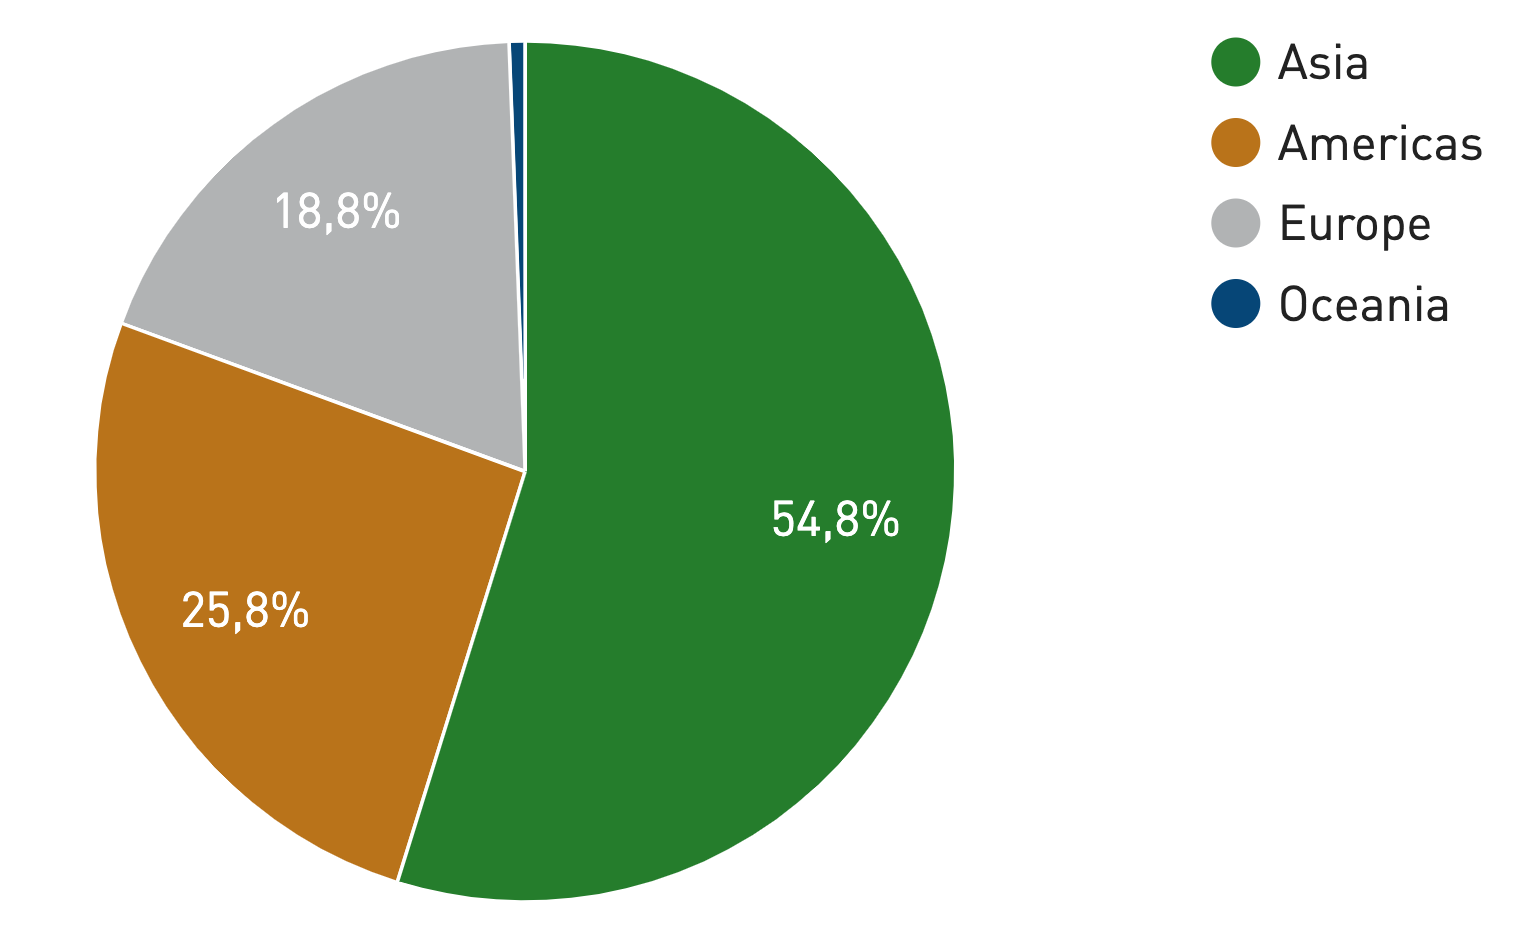
\includegraphics[width=10cm]{images/edl_top500_continent.png}
        \caption{\label{fig:edl_top500_continent} Répartition de la puissance de calcul du Top500 de novembre 2019 entre les continents.}
    \end{figure}
    
    
    Pour accélérer le développement de ses infrastructures, l’Europe a financé un grand projet nommé Horizon 2020. Horizon 2020 est le plus grand programme de recherche et d'innovation jamais mis en place par l'Union européenne. Ce projet d’envergure prévoit d’investir 79 milliards d’euros de 2014 à 2020 pour développer trois piliers : l'excellence scientifique, la primauté industrielle et les défis sociétaux.
    En janvier 2018, la Commission européenne a annoncé investir 1 milliard dans un partenariat réalisé entre le domaine public et privé nommé EuroHPC \cite{EuroHPC2018}. Les objectifs d'EuroHPC sont de développer et déployer une infrastructure de calcul de classe mondiale. 
    Cette entreprise communautaire aura pour objectif de construire 6 supercalculateurs: 2 supercalculateurs petascale ($10^{16}$ opérations) et deux infrastructures ``\textit{pré exascale}'' en 2021. Les architectures pré exascale vont permettre d'utiliser les premières versions des processeurs développées par EuroHPC. Pour assurer son indépendance technologique, le projet EPI (\textit{European Processor Initiative}) a pour objectif de développer de nouveaux processeurs et des accélérateurs MPPA (\textit{massively parallel processor array}) produits par Kalray à Grenoble (voir \autoref{fig:edl_epi_processor}). Enfin, le supercalculateur exaflopique européen prévu entre 2022 et 2023 pourra compter sur de nouvelles architectures, très efficaces énergétiquement, basées sur des processeurs ARM actuellement en développement. Une des motivations étant de réduire sa dépendance aux autres pays pour être plus compétitif.  

    \begin{figure}
        \center
        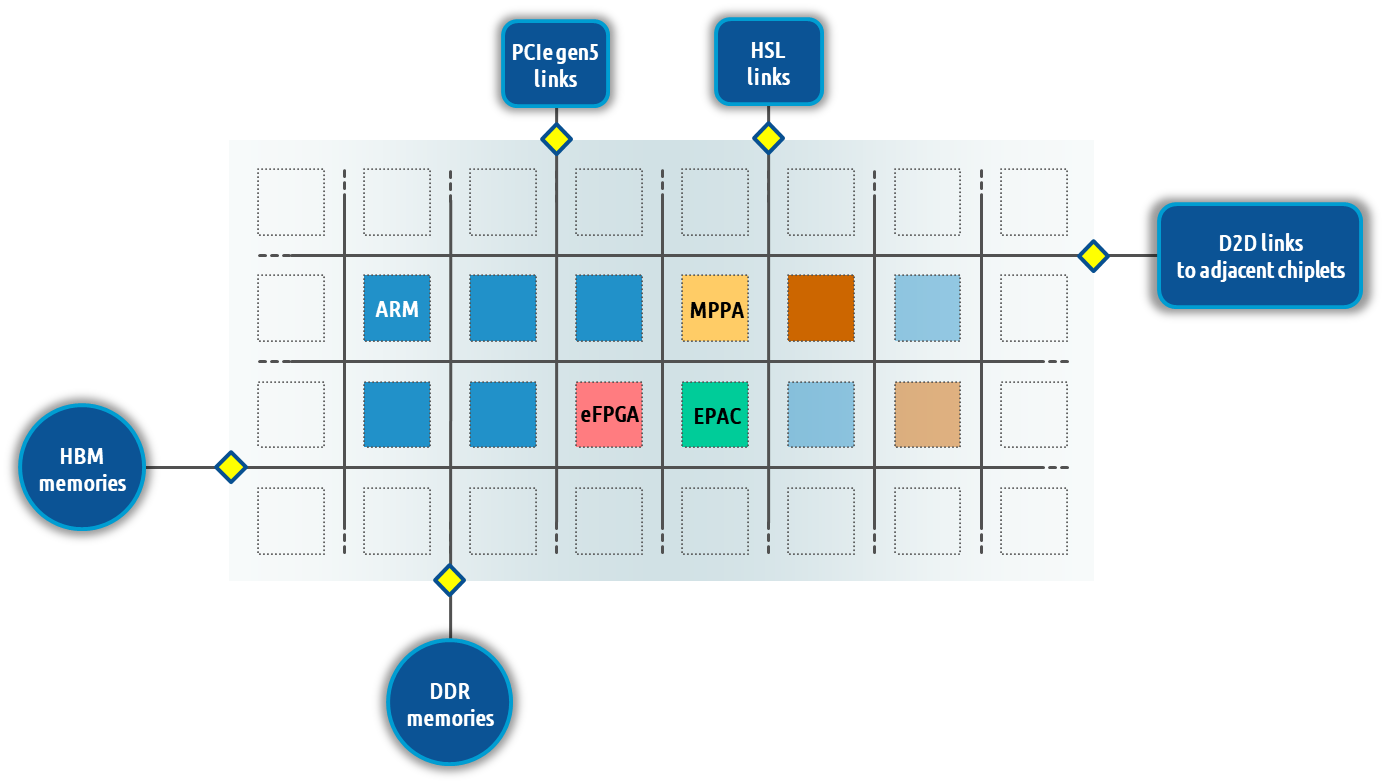
\includegraphics[width=14cm]{images/edl_epi_processor.png}
        \caption{\label{fig:edl_epi_processor} Les processeurs GPP utiliseront un réseau à mailles 2D sur la puce permettant de relier différents types de coeurs: ARM-V, FPGA embarqué (eFPGA) pouvant être reprogrammé, un processeur vectoriel (MPPA).}
    \end{figure}
    
    
    \paragraph{Les États-Unis.}
    En 2017, le département de l'énergie américain a annoncé le financement d'un projet de 232 millions d'euros nommé PathForward. Ce budget est réparti entre 6 entreprises américaines (HPE, AMD, Cray, IBM, Intel et Nvidia) qui doivent ajouter 40\% de financement supplémentaire pour un total de plus de 400 millions d'euros. L'objectif de ce projet est de construire le premier ordinateur \gls{exascale} en 2021 en finançant les développements matériels et logiciels nécessaires.


        
    %%%%%%%%%%%%%%%%%%%%%%%%%%%%%%%%%%%%%%%%%%%


\subsection{Nouvelles technologies mémoire.}\label{sec:oppo_new_memory}
%%%%%%%%%%%%%%%%%%%%%%%%%%%%%%%%%%%%%%%%%%%%%%%%%%        

     
    Dans cette section, nous utilisons le terme \textit{gap} pour traduire un écart de performance entre deux technologies. Le terme ``\gls{memorygap}'' est couramment utilisé dans la littérature pour désigner l'écart de performance actuel entre les processeurs et le système mémoire \cite{Wilkes2001}.

    %HISTORIQUE: evo + memory Gap 
    \subsubsection{Memory gap: état des lieux des technologies}
    
        L'évolution des capacités opérationnelles des processeurs et de la performance des mémoires (débits, latence, taille) a été très inégale. La \autoref{fig:edl_memory_pyramide} présente sous forme de pyramide les différentes technologies mémoire actuellement utilisées dans le système. Les trois principaux facteurs différenciant les différentes technologies mémoire sont: le prix, la latence d'accès et la capacité (densité). Pour mieux appréhender la différence de latence des technologies, nous les convertissons dans un temps plus facilement appréciable pour un humain. Si un accès au cache L1 prenait 3 secondes, un accès mémoire prendrait alors plus de 5 minutes. Si la donnée à récupérer se trouve sur un disque SSD, il faudrait attendre 3 heures avant de la recevoir. Si celle-ci se trouve sur un disque optique, il faudrait alors patienter 10 mois. Il est facile de comprendre pourquoi le \textit{manque} (\textit{miss}) d'une donnée dans le cache pénalise énormément la performance d'une application. 
        
        \begin{figure}
            \center
            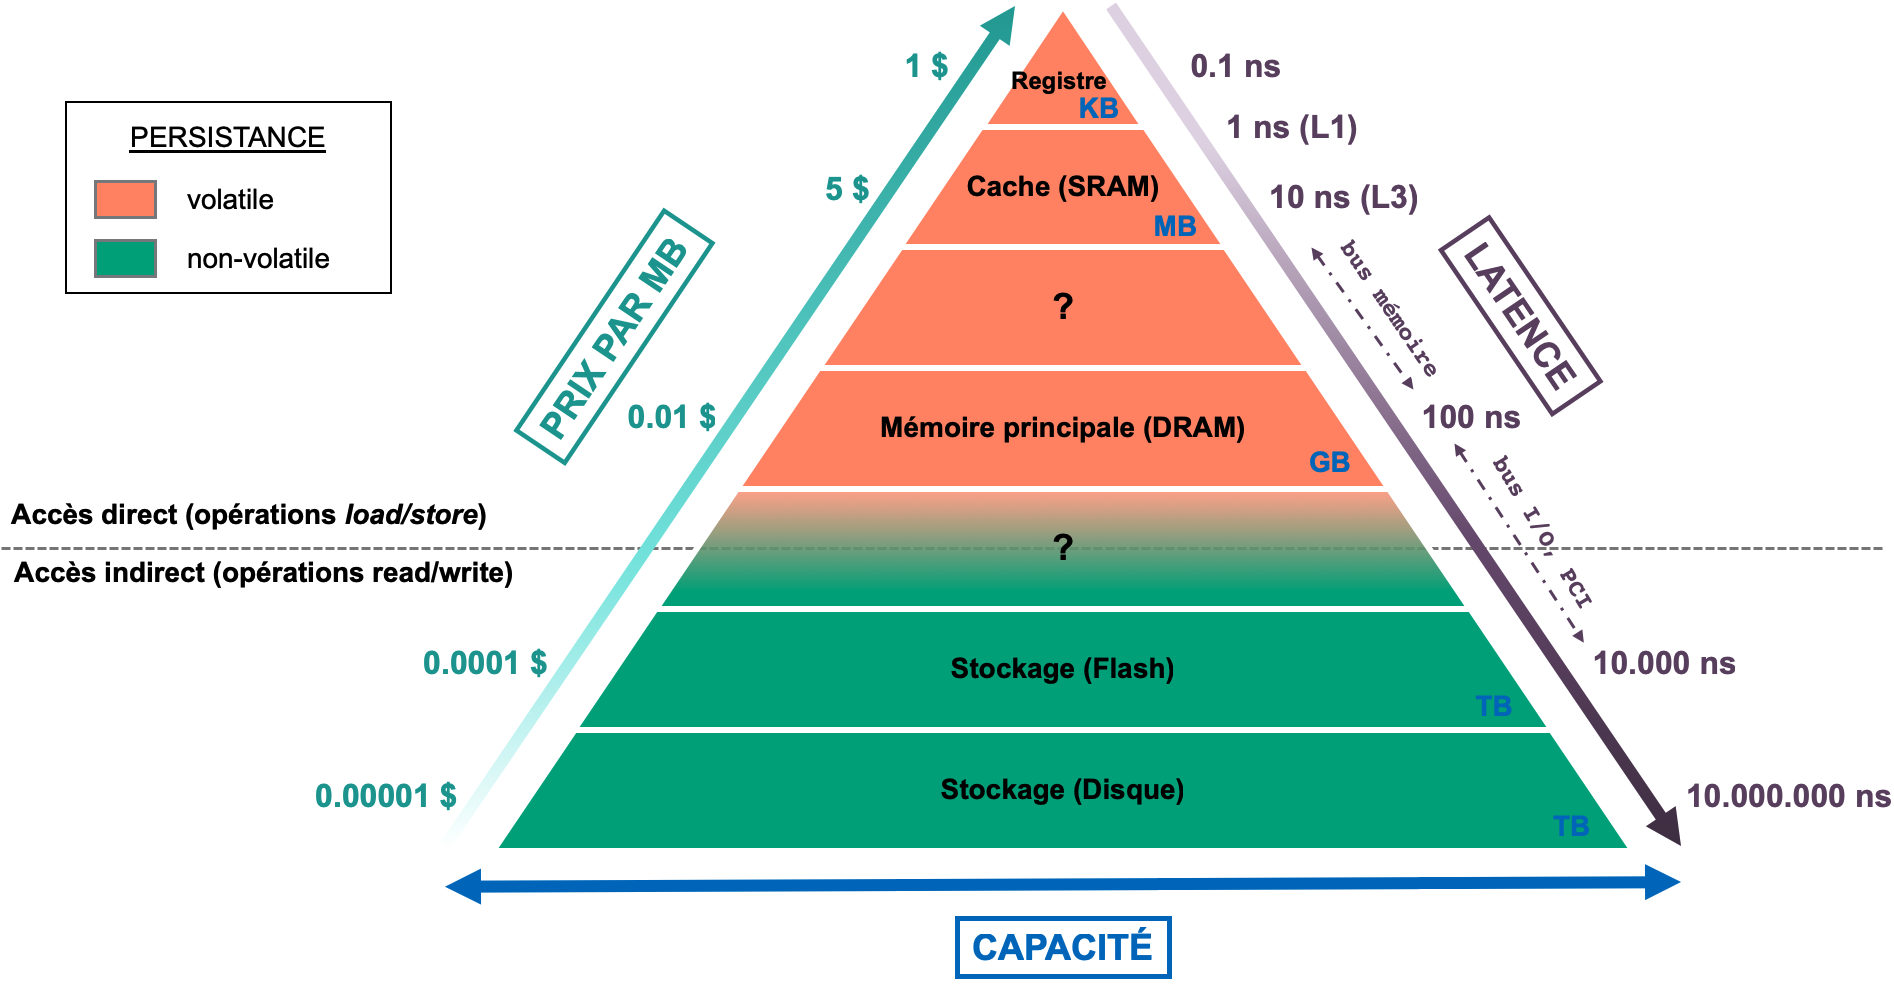
\includegraphics[width=17cm]{images/edl_memory_pyramide.png}
            \caption{\label{fig:edl_memory_pyramide} Hiérarchisation des différents types de mémoire en fonction du coût, de la latence et de la capacité de stockage habituellement utilisés dans les architectures modernes. Les écarts de performance relevés dans la hiérarchie mémoire sont modélisés par un '?'.}
        \end{figure}
        
        Malgré le développement d'une hiérarchie mémoire (voir \autoref{sec:hierarchie}) pour réduire ces écarts de performance, nous remarquons  la présence de deux \textit{trous} (\textit{memory gap}) de performance. Pour résoudre ce problème, l'industrie poursuit le travail débuté avec l'introduction de la hiérarchie mémoire grâce à deux solutions: 
        \begin{itemize}
            \item Réaliser le traitement directement dans la mémoire grâce aux techniques de calculs en mémoire (\textit{processing-in memory} (PIM)) \cite{Singh2019}. En déplaçant le calcul en mémoire, les latences d'accès sont réduites et les débits augmentés. Des implémentations d'architecture PIM utilisent des mémoires SRAM qui ont permis d'accélérer des algorithmes d'apprentissage machine \cite{Zhang2016, Biswas2018, Kang2018}. D'autres implémentations utilisent de la mémoire DRAM \cite{Seshadri2017} \cite{Li2017} permettant de réaliser des opérations logiques \verb|AND| et \verb|OR| sur des  barrettes mémoires DRAM classiques non modifiées \cite{Gao2019}. Des technologies comme le memristor permettent de réaliser des multiplications de matrices dont chaque valeur peut être calculée simultanément. Ce composant électronique a été décrit par Leon Chua en 1971 dans l'article ``\textit{ Memristor - The Missing Circuit Element}''  \cite{Chua1971}. La première implémentation physique a été réalisée par une équipe de recherche des laboratoires d'HP conduite par Stanley Williams en 2008 et publiée dans l'article ``\textit{The missing memristor found}'' \cite{Strukov2008}. Cette mémoire permet d'encoder un nombre réel sur un seul bit. L'information encodée peut ainsi avoir une infinité de valeurs contrairement à deux valeurs pour les bits des mémoires utilisées habituellement.
            
            \item La deuxième solution permettant d'accélérer les accès mémoire est de combler les deux \textit{trous} de performance constatés sur la \autoref{fig:edl_memory_pyramide} grâce au développement de nouvelles technologies mémoire. Les différentes solutions envisagées sont discutées dans le reste de cette section.
        \end{itemize}
        
        
    
    
    \subsubsection{Trou entre SRAM et DRAM} 
        Pour réduire le trou séparant les mémoires cache et la mémoire centrale, les processeurs ont vu leur dernier niveau de cache s'agrandir. Cependant, la mémoire SRAM utilisée est très chère à produire et sa densité ne permet plus d'agrandir la capacité des mémoires cache. Côté mémoire principale, le développement de différentes technologies mémoire (DDR3, DDR4, DDR5) ne permet pas de faire évoluer fortement la performance des applications. La raison principale vient de la difficulté à augmenter le débit du bus mémoire qui est limité par le nombre de broches utilisables sur le processeur. La \autoref{fig:edl_channel_pin} montre l'évolution de la proportion de broches d'un processeur qui est affectée au bus mémoire. Il est aujourd'hui très difficile d'allouer plus de broches pour le bus mémoire. Le nombre de canaux a augmenté, permettant d'améliorer le débit du bus mémoire. Cependant, le nombre de coeurs a lui aussi évolué, bien plus rapidement que le nombre de canaux mémoire. Ainsi, la bande passante mémoire par coeur est passée de 6.4 Gb/s pour un processeur de 8 coeurs en 2012 à 4.6 Gb/s pour un processeur de 28 coeurs en 2016. 
        
        \begin{figure}
            \center
            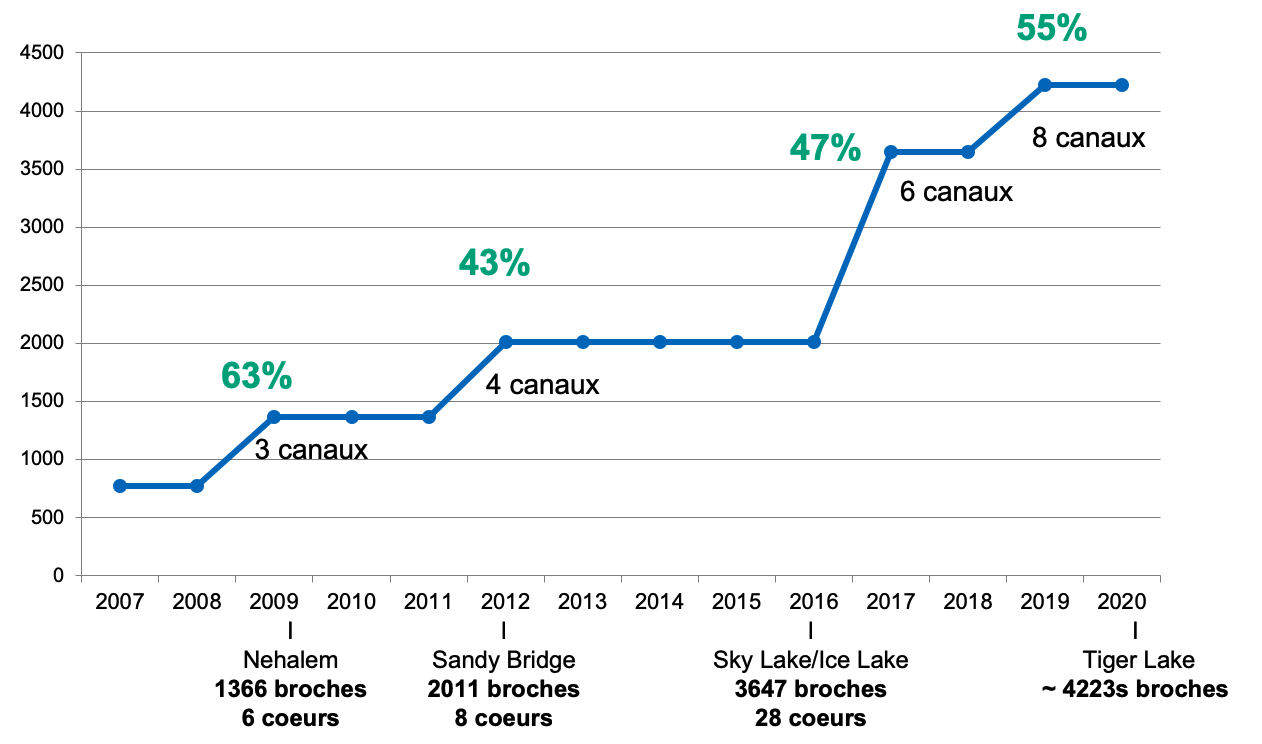
\includegraphics[width=12cm]{images/edl_channel_pin.png}
            \caption{\label{fig:edl_channel_pin} Nombre et proportion de broches allouées aux bus mémoires des dernières architectures de processeur Intel.}
        \end{figure}
    
    
        À partir de ce constat, et celui fait dans la \autoref{sec:edl_chal_energie} concernant la consommation énergétique du système mémoire, les architectures ont été repensées pour placer la mémoire directement sur les puces (\textit{On Package Memory}) au plus proche des circuits de traitement (\textit{near-memory processing}). En plaçant la mémoire directement sur la puce du processeur, les limitations imposées par le bus mémoire (débit, consommation électrique) peuvent être contournées notamment grâce à l'utilisation de bus plus large (voir \autoref{fig:edl_hbm_vs_gddr5}). Afin de pouvoir installer des espaces mémoire suffisamment larges directement sur la puce, un nouveau type de mémoire a été développé: les mémoires 3D. La principale différence avec la mémoire conventionnelle est son architecture qui est en 3D. Alors que la mémoire DRAM s’étale sur deux dimensions X, Y, la mémoire 3D s’étend en plus sur une troisième dimension Z en s’empilant (\textit{stack}, voir \autoref{fig:edl_hbm_precis}). En empilant des couches de silicium, ces mémoires sont très denses. Ainsi, 1GB de GGDR5 qui nécessite $672 mm^2$, n'a besoin que de $35 mm^2$ pour la même capacité de mémoire 3D, soit une réduction de 94\%\footnotetext{Mesure réalisée par AMD sur 1GB GDDR5 (4x256MB ICs) et 1GB HBM-2 (1x4-Hi)}. 
        
                   
        
        \begin{figure}[t!]
            \centering
            \begin{subfigure}[t]{0.48\textwidth}
                \centering
                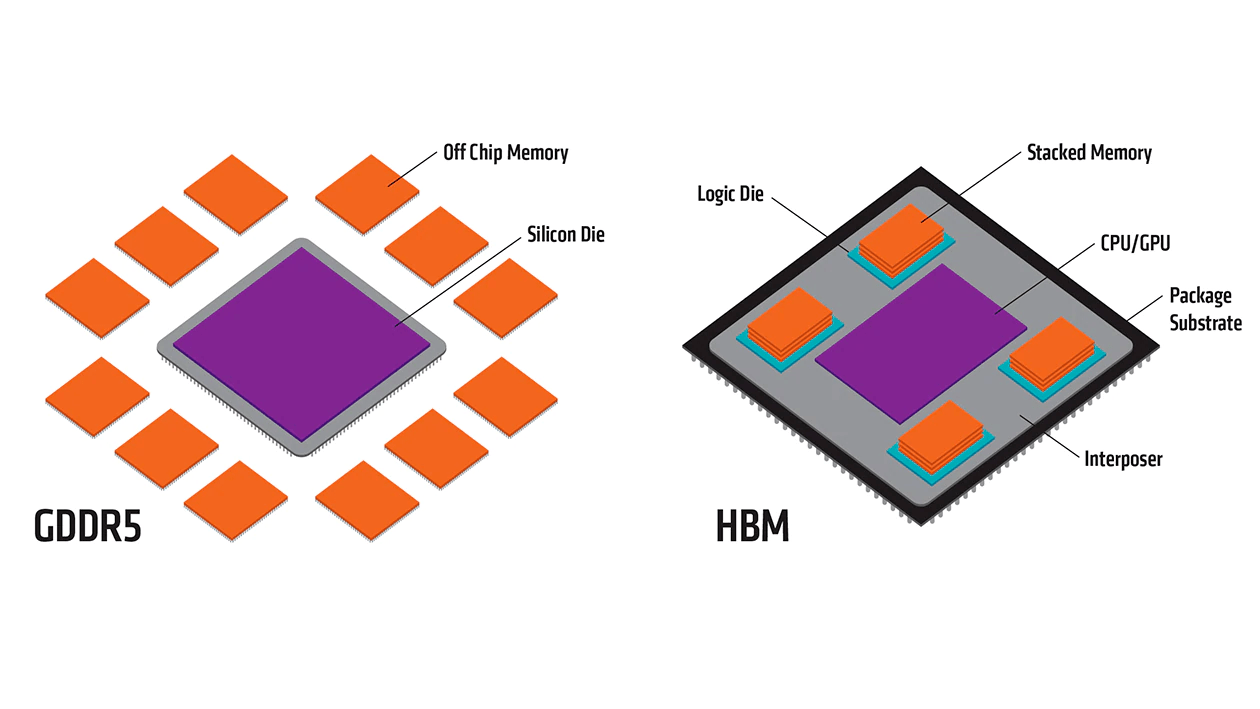
\includegraphics[width=\linewidth]{images/edl_hbm_vs_gddr5.png}
                \caption{\label{fig:edl_hbm_vs_gddr5} Pour atteindre de meilleures performances, les mémoires 3D sont placées directement sur la puce.}
            \end{subfigure}\hfill
            \begin{subfigure}[t]{0.48\textwidth}
                \centering
                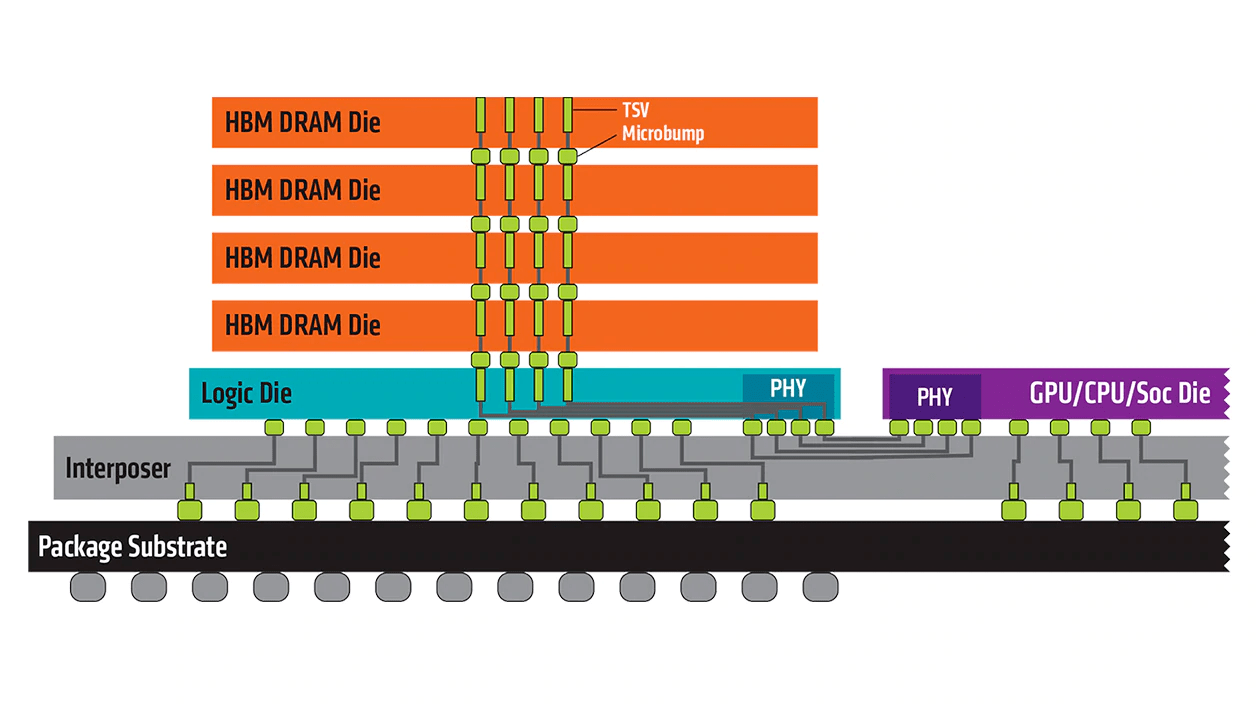
\includegraphics[width=\linewidth]{images/edl_hbm.png}
                \caption{\label{fig:edl_hbm_precis} Les mémoires 3D sont un empilement de mémoire DDR relié à un interposeur grâce à des \textit{vias} (TSV, TCI).}
            \end{subfigure}
            \caption{\label{fig:edl_hbm}Architecture et utilisation d'une mémoire 3D sur un GPU\protect\footnotemark}
        \end{figure}
        \footnotetext{Source AMD - \url{https://www.amd.com/fr/technologies/hbm}}
        
        
        Actuellement, les mémoires 3D sont principalement commercialisées sous les technologies HBM (\textit{High Memory Bandwidth} \cite{Standard2013}) produite par AMD, Samsung et Hynix et de la HMC (\textit{Hybrid Memory Cube}\cite{Jeddeloh2012}) produite par Micron. Les mémoires HBM se composent actuellement de quatre puces DRAM sur une puce de base et possèdent deux canaux de 128 bits par puce DRAM, soit 8 canaux au total, ce qui donne 1024 bits par pile d'interfaces mémoire (voir \autoref{tab:hmb2_vs_grrd5}). Une carte graphique possédant 4 piles possède ainsi un bus mémoire de 4096 bits. Pour améliorer l'efficacité énergétique, la fréquence des mémoires 3D est moins rapide que celle des mémoires DRAM conventionnelles. De plus la proximité de ces mémoires dites \textit{on-package}, permet de réduire la distance de communication avec les processeurs et de réduire la consommation électrique (3.9 pJ/bit pour la HBM2 contre 14 pJ/bit pour la GDDR5). Malgré une fréquence plus faible, le large bus mémoire directement connecté à la puce permet d'atteindre des bandes passantes plus élevées. Pour une enveloppe énergétique de 60W, une mémoire GDDR5 est capable de fournir un débit de 536 Gb/s quand une mémoire HBM2 peut atteindre 1.9 Tb/s \cite{OConnor2017}. Les mesures de performances réalisées à l'aide du benchmark Stream ont permis de mesurer des écarts de performances d'un facteur 4 avec une mémoire DDR4 classique\cite{7965110}, tout en consommant 50\% d'énergie en moins \footnotetext{Information NVIDIA - \url{https://www.extremetech.com/extreme/226240-sk-hynix-highlights-the-huge-size-advantage-of-hbm-over-gddr5-memory}}. Cependant, des latences d'accès réduites (15\%) ont été mesurées et peuvent impacter la performance de certaines applications. L'utilisation de nombreux coeurs et d'instructions de préchargement mémoire peuvent cependant permettre d'atteindre de meilleurs résultats \cite{7965110}.
        
        % Please add the following required packages to your document preamble:
        % \usepackage{graphicx}
        \begin{table}[]
        \centering
        \resizebox{\textwidth}{!}{%
        \begin{tabular}{|l|c|c|c|c|c|c|}
        \hline
        & \textbf{Largeur bus} & \textbf{Capacité (GB)} & \textbf{Débit (Gb/s)} & \textbf{Fréquence mémoire} & \textbf{Bande passante (Gb/s)} & \textbf{Consommation (pJ/bit)} \\ \hline
        \textbf{GDDR5} & 768 & 24 & 8 & 1.25 GHz & 480 & 14 \\ \hline
        \textbf{HBM2} & 4096 & 8 & 2 & 1 GHz & 1024 & 4 \\ \hline
        \end{tabular}%
        }
        \caption{Comparaison des mémoires GDDR5 utilisées sur les GPU NVidia K80 et des mémoires HBM2 utilisées sur un GPU utilisant 4 piles de mémoire.}
        \label{tab:hmb2_vs_grrd5}
        \end{table}
         
    \subsubsection{Trou entre DRAM et Flash}
    %%%%%%%%%%%%%%%%%%%%%%%%%%%%%%%%%%%%%%%

        %INTRO
        La nécessité d'augmenter les capacités de stockage, la pression énergétique et la faiblesse d'évolution des performances du système mémoire sont à l'origine du développement de nouvelles technologies visant à combler le trou situé entre la mémoire et le stockage. L'utilisation de ces nouvelles mémoires n'est pas seulement une évolution de performance. Elles vont aussi permettre de développer de nouvelles approches logicielles. Par exemple, lors de l'arrêt d'un ordinateur, si la totalité de la mémoire y est sauvée, le temps de redémarrage sera accéléré. Les applications telles que les bases de données relationnelles sont développées pour anticiper les longues latences des disques pourront être stockées directement en mémoire, sans risque de perdre l'informations (\textit{In memory database} \cite{Oukid2015}). Les applications de simulations numériques pourront rapidement générer des points de contrôle (\textit{checkpoint}), permettant de reprendre le traitement suite à une erreur. 
        
        %En plus des performances, plusieurs spécificités séparent la mémoire principale du stockage:
        %\begin{itemize}
         %   \item L'adressabilité: En mémoire, chaque octet est adressable alors que les disques sont adressés par blocs de plusieurs octets (généralement 512 octets).
          %  \item Les opérations: En mémoire le processeur peut directement travailler sur les données grâce aux opérations \textit{load/store}. Le stockage est lui géré par des opérations d'entrée/sortie telles que \textit{read/write}.
           % \item La persistance: lorsque le courant est coupé, les données présentes en mémoire sont effacées contrairement au stockage.
        %\end{itemize}
        
        %Critère
        
        L'objectif est donc de développer de nouvelles mémoires ayant les avantages des deux technologies (DRAM et flash) sans leurs inconvénients. Plusieurs critères sont alors essentiels pour leur adoption (\cite{Freitas2008}). Le premier  concerne la persistance des données, permettant entre autres de réduire leur consommation énergétique. Pour des raisons de fiabilité et de densité, ces mémoires ne doivent pas contenir de parties mobiles telles qu'un disque rotatif. Pour être utilisées comme mémoire, ces nouvelles technologies doivent pouvoir atteindre des latences d'accès faibles (autour de 200 ns\cite{IBM2013}), proches de celle de la DRAM. Les technologies développées doivent être endurantes pour pouvoir être utilisées intensivement (entre $10^9$ et $10^{12}$ écritures par cellule \cite{IBM2013}). À terme, ces technologies devraient remplacer les mémoires DRAM, elles doivent donc être adressables par octet. Enfin, pour être accepté par l'industrie, le prix de ces mémoires doit être compétitif avec les technologies existantes. Avec les critères exposés précédemment, nous constatons qu'il n'est pas possible de compter sur les technologies existantes:
        \begin{itemize}
            \item Les disques optiques permettent d'obtenir de grandes capacités de stockage. Cependant, à cause des parties mécaniques (disques rotatifs, bras de lecture) les latences et les débits sont trop faibles. De plus, pour obtenir des latences acceptables, les disques doivent tourner continuellement, augmentant leur consommation énergétique et réduisant leur fiabilité.
            \item La technologie flash ne possède pas une endurance aux écritures suffisante ($10^6$ écritures), loin des objectifs fixés ($10^9$ écritures). De plus, par héritage de la technologie des disques optiques, les disques SSD ne sont adressables que par bloc.
            \item La mémoire DRAM possède de très bonnes performances en lecture comme en écriture. Cependant, sa densité est faible et elle doit constamment être alimentée pour conserver ses données, augmentant la consommation électrique.
        \end{itemize}
        %: la densité, la volatilité et le prix des disques associé à latences et l'endurance de la mémoire. 
  
        
    
        
        %DEFINITION SCM
        \paragraph{NVM, NVRAM ou SCM ?}
            
            De nombreux termes sont utilisés dans la littérature pour désigner ces nouvelles mémoires: NVM (\textit{non-volatile memory}), NVRAM (\textit{non volatile RAM}) ou encore PM (\textit{persistent memory}). Le terme NVM est souvent confondu avec le terme NVMe qui désigne un nouveau protocole de communication visant à remplacer le protocole SATA. Les différentes implémentations des NVRAM sont présentées sur la \autoref{fig:memoire_stockage_def}. Le premier critère de classement est celui de la volatilité puis de l'adressabilité. La seule NVRAM couramment utilisée qui n'est adressable qu'en bloc est la mémoire flash, ne répondant ainsi pas au critère d'adressabilité fixé ci-dessus. Il y a ensuite deux façons d'implémenter des NVRAM adressables par octet: les NVDIMM (Non-Volatile DIMM), les SCM (\textit{Storage Class Memory}).
            
            
            \begin{figure}
                \center
                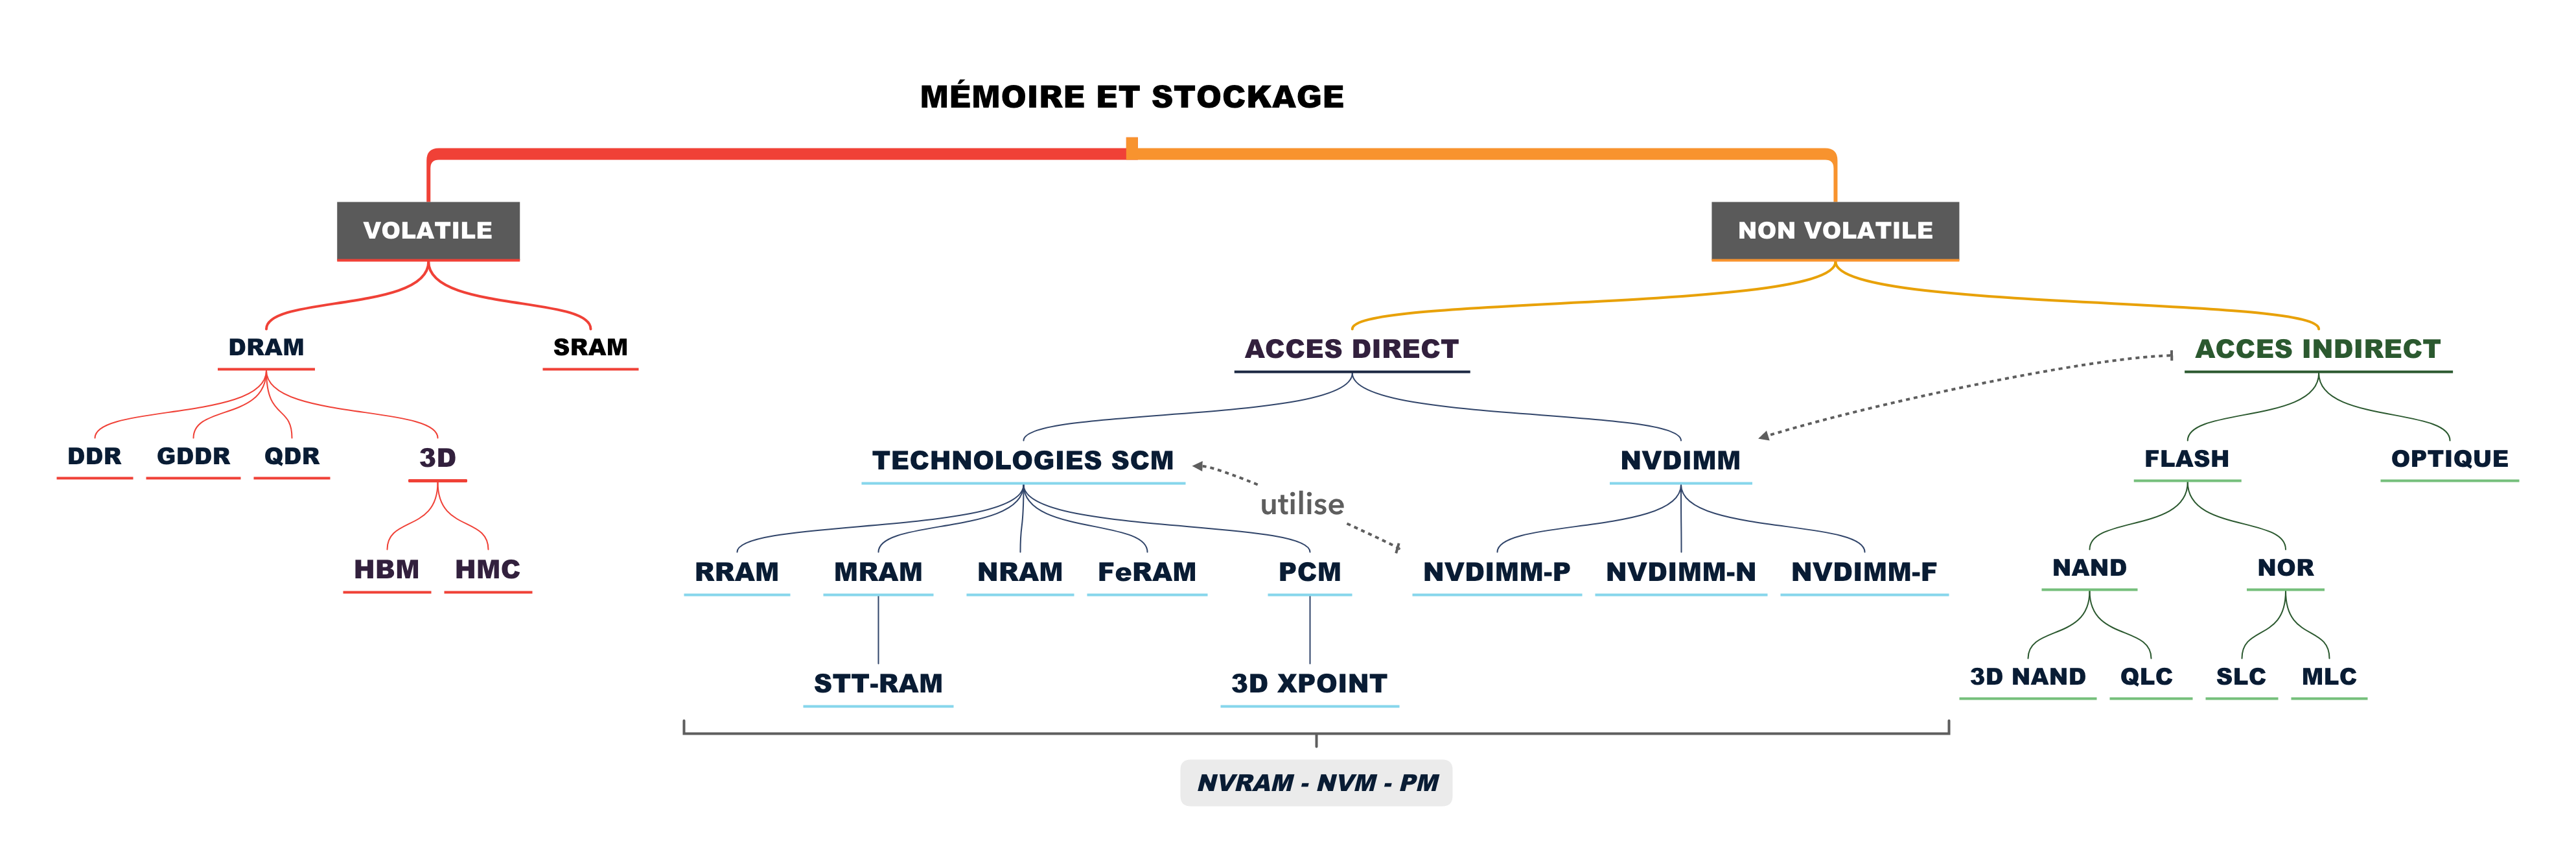
\includegraphics[width=17cm]{images/memoire_stockage_def.png}
                \caption{\label{fig:memoire_stockage_def} Tri des technologies de stockage en fonction de la volatilité et l'adressabilité.}
            \end{figure}
    
    
    %%%%%%%%%%%%%%%%%%%%%%%%%%%%%
    
    \paragraph{Les NVDIMM.}\label{sec:nvdimm}
    
        La NVDIMM est une technologie mémoire qui utilise le même format que les barrettes de mémoires classiques DRAM \cite{ChrisEvans2017}, elle peut donc être adaptée sur les serveurs actuels. Le système d'exploitation doit cependant être adapté pour profiter des avantages de la persistance et être, par exemple, capable de redémarrer directement à partir des données se trouvant en mémoire (les versions supérieures à Linux 4.4 sont compatibles). L'organisation JEDEC\footnote{JEDEC - \url{https://www.jedec.org/}} a été créée en 1958 et développe, entre autres, les standards utilisés en micro électronique. L'organisation a publié 3 standards pour le développement des NVDIMM (voir \autoref{fig:edl_nvdimm}).
    
            \begin{figure}[t!]
                \centering
                \begin{subfigure}[t]{0.50\textwidth}
                    \centering
                    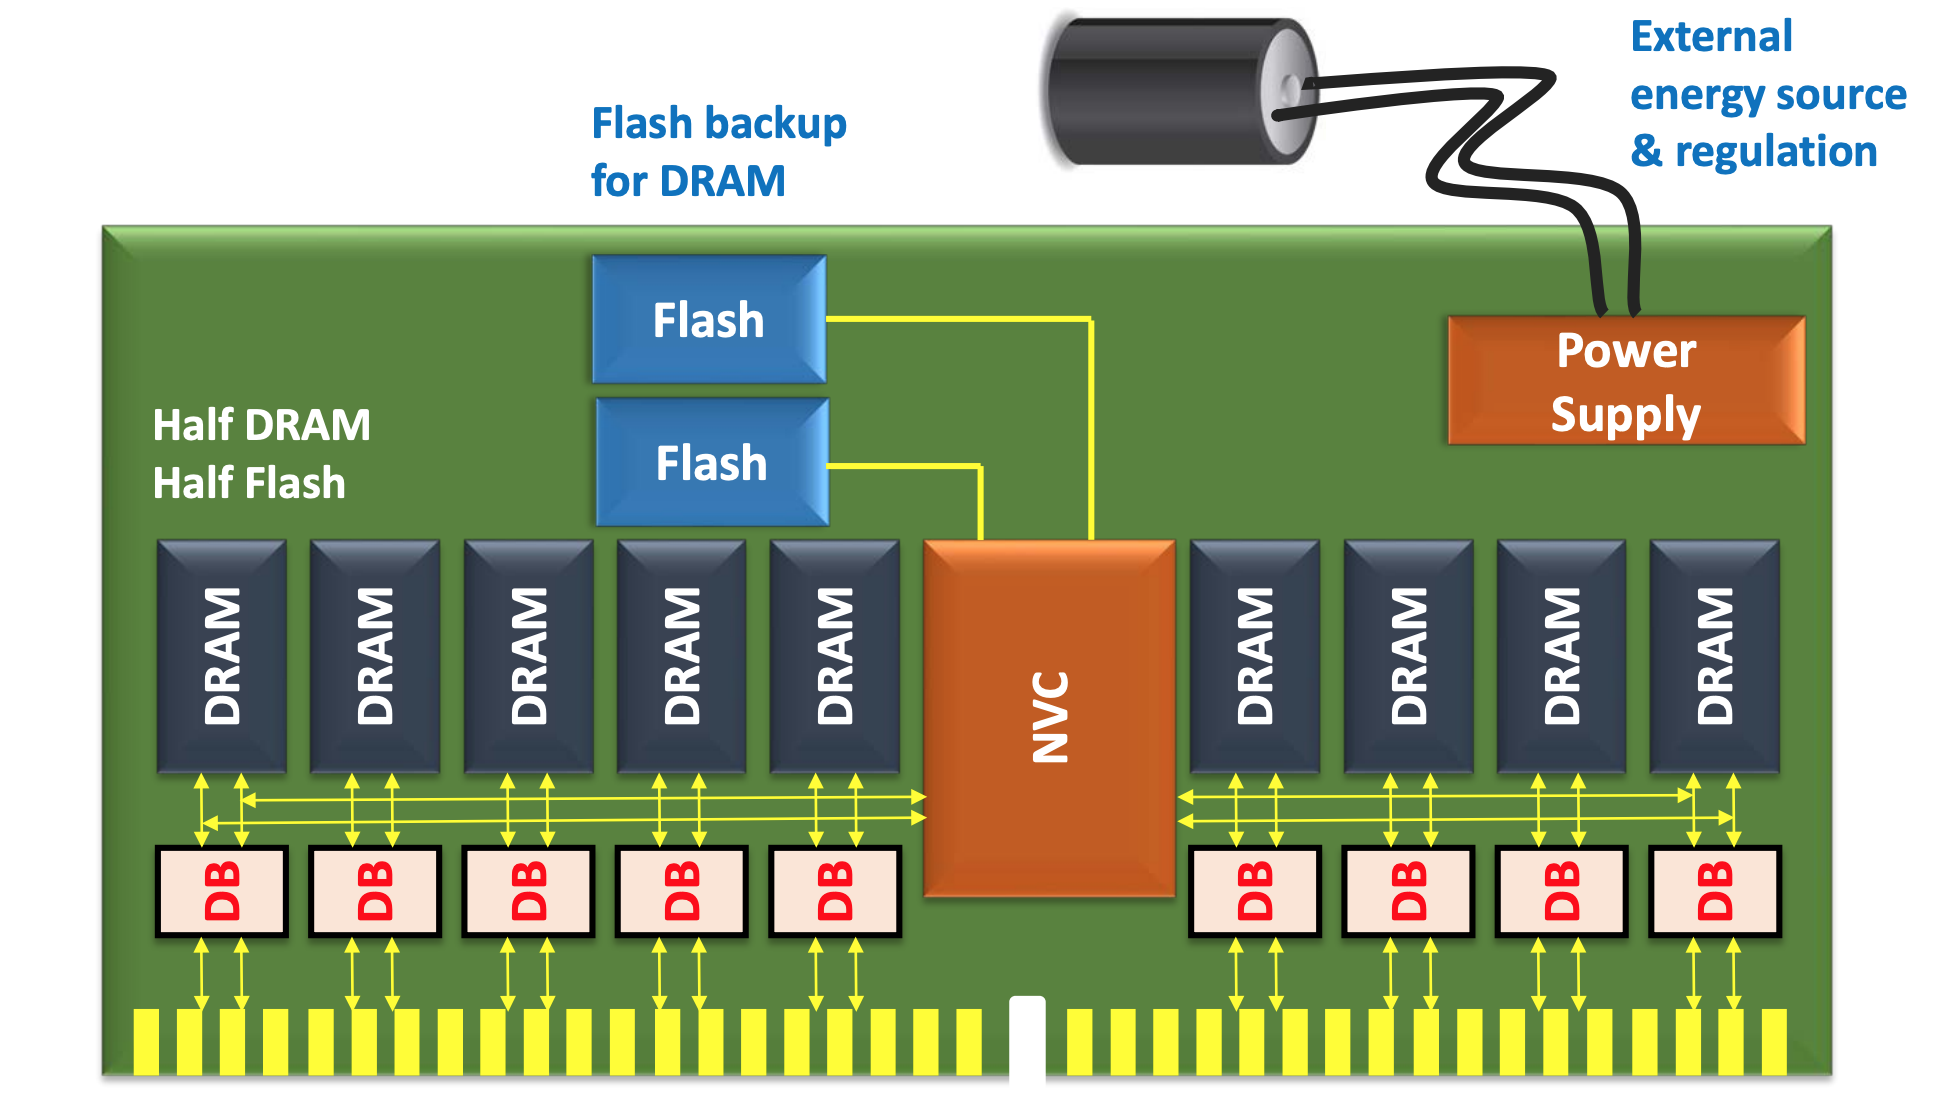
\includegraphics[width=\linewidth]{images/edl_nvdimm_n.png}
                    \caption{\label{fig:edl_nvdimm_n} NVDIMM-N}
                \end{subfigure}\hfill
                \begin{subfigure}[t]{0.50\textwidth}
                    \centering
                    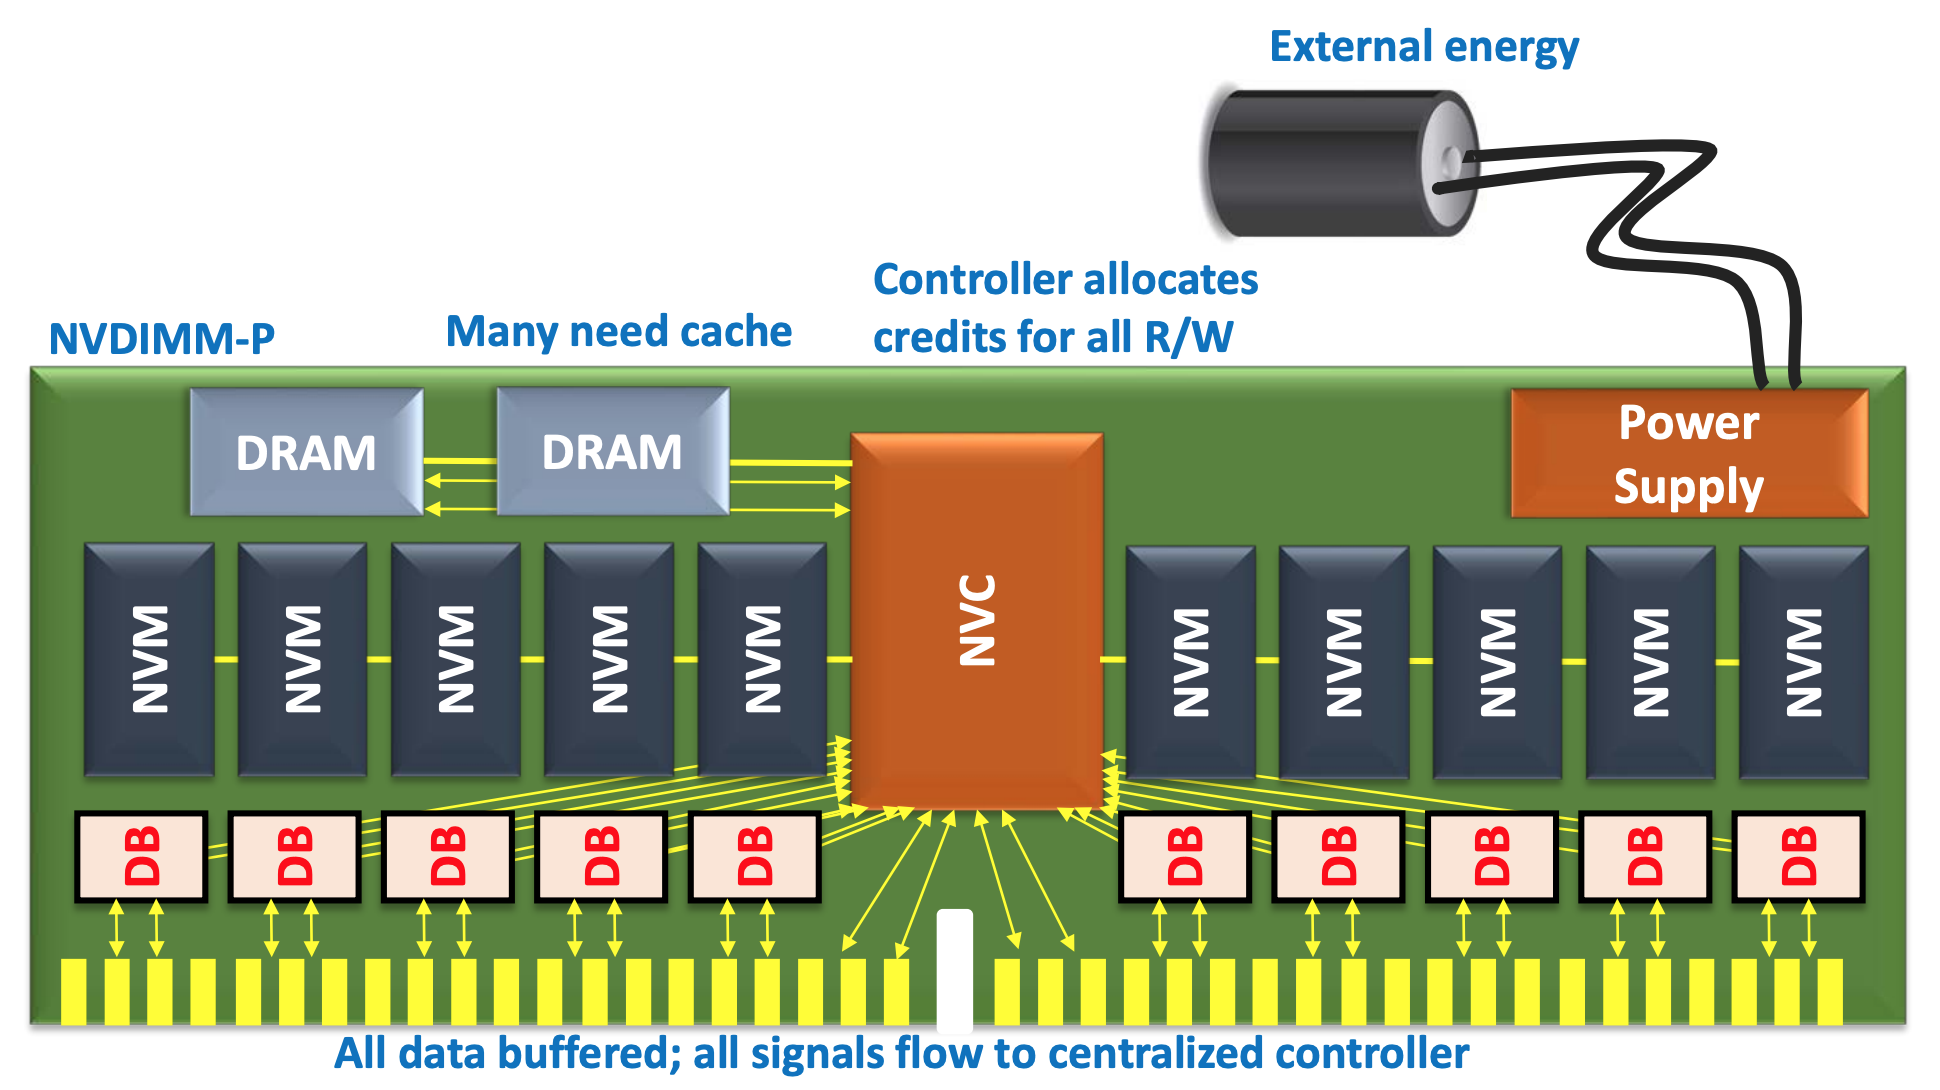
\includegraphics[width=\linewidth]{images/edl_nvdimm_p.png}
                    \caption{\label{fig:edl_nvdimm_p}NVDIMM-P}
                \end{subfigure}
                \caption{\label{fig:edl_nvdimm}Les deux standards NVDIMM développés par l'organisation JEDEC\protect\footnotemark.}
            \end{figure}
            \footnotetext{Source des illustrations: Bill Gervasi (Nantero) - \url{https://www.hotchips.org/hc30/2conf/2.04_Nantero_20180818_hotchips_gervasi_nram_presentation.pdf}}
        
        Le premier standard (Type 1) appelé NVDIMM-N (voir \autoref{fig:edl_nvdimm_n}) utilise de la mémoire DRAM associée à de la mémoire flash pour permettre la persistance des données ainsi qu'une source d'énergie indépendante permettant la sauvegarde des données en cas de coupure électrique. Lorsque le serveur est de nouveau alimenté, les données sont transférées de la mémoire flash à la DRAM pour permettre un redémarrage rapide. Pour l'utilisateur, la mémoire flash est invisible et ne peut pas être adressée. La capacité de ces mémoires aura tendance à être faible, car elles dépendent de la densité de la mémoire flash. Cependant, si la mémoire DRAM est bien utilisée, elle permet d'obtenir des performances et une endurance aux écritures proches d'une barrette de mémoire classique et bénéficie de la persistance grâce à la mémoire flash. 
            
        Le second standard (Type 3) appelé NVDIMM-F utilise seulement de la mémoire flash et est présenté au système d'exploitation comme un stockage. Cependant, contrairement à un disque classique, il bénéficie des performances du bus mémoire. Ce standard a depuis été abandonné. 
        
        Le troisième standard (Type 4) appelé NVDIMM-P (voir \autoref{fig:edl_nvdimm_p}) utilise de la mémoire DRAM associée à des technologies mémoire SCM (voir paragraphe suivant). Ces barrettes utilisent des banques de mémoires DRAM comme cache pour accélérer les communications avec les modules SCM. Le standard prévoit la possibilité d'adresser la mémoire en octets ou en blocs permettant de les utiliser comme mémoire, ou comme stockage. Les performances et la capacité de ce format de barrettes dépendent essentiellement des technologies SCM utilisées. C'est un avantage de ce type de NVDIMM, la technologie et le mode d'adressage utilisés pourront être adaptés en fonction des besoins des applications. Bien que la mémoire SCM soit non volatile, la barrette mémoire nécessite une alimentation pour sauvegarder le contenu de la DRAM sur la SCM en cas de coupure électrique.

    \paragraph{Les Storage Class Memory (SCM)}\label{sec:SCM}
    %%%%%%%%%%%%%%%%%%%%%%%%%%%%%%%%%%%%%%%%%%%%%%%%%
    
        Les mémoires SCM regroupent toutes les nouvelles technologies développées répondant aux critères précédemment cités. La mémoire flash peut être considérée comme une SCM. Cependant, dans la littérature, le terme SCM est généralement utilisé pour désigner des technologies très innovantes aux caractéristiques supérieures à la mémoire flash. Cette technologie possède en effet quelques inconvénients qui ne permettront pas de l'utiliser comme une mémoire. Tout d'abord, ses performances asymétriques dont l'écriture est dix fois plus lente que la lecture. L'écriture et l'effacement ne peuvent se faire que par bloc. Enfin, l'endurance de la mémoire flash ne permet pas de supporter suffisamment d'écriture par cellule. En fonction des technologies utilisées (SLC, MLC, TLC), le nombre d'écritures par cellule est compris entre $10^3$ et $10^5$.  
        
        
        Dans la suite de cette section, nous présentons les technologies SCM ayant le plus de potentiel pour être industrialisées. En fonction des utilisations, certains types de mémoires seront préférés. Pour des applications de stockage, leur coût devra être proche de celui des disques, mais pourra avoir des latences plus élevées (inférieur à la microseconde) et des débits plus faibles (en centaines de mégaoctets/s). Cependant, leur endurance devra être la plus élevée possible ($10^{12}$ écritures). À terme, le prix des mémoires SCM devrait converger vers celui des mémoires flash, permettant une utilisation massive dans les systèmes (voir \autoref{fig:edl_scm_evo}). Nous regroupons dans le \autoref{tab:SCM} les principales caractéristiques de ces technologies.
        
        
        \begin{figure}
        \center
        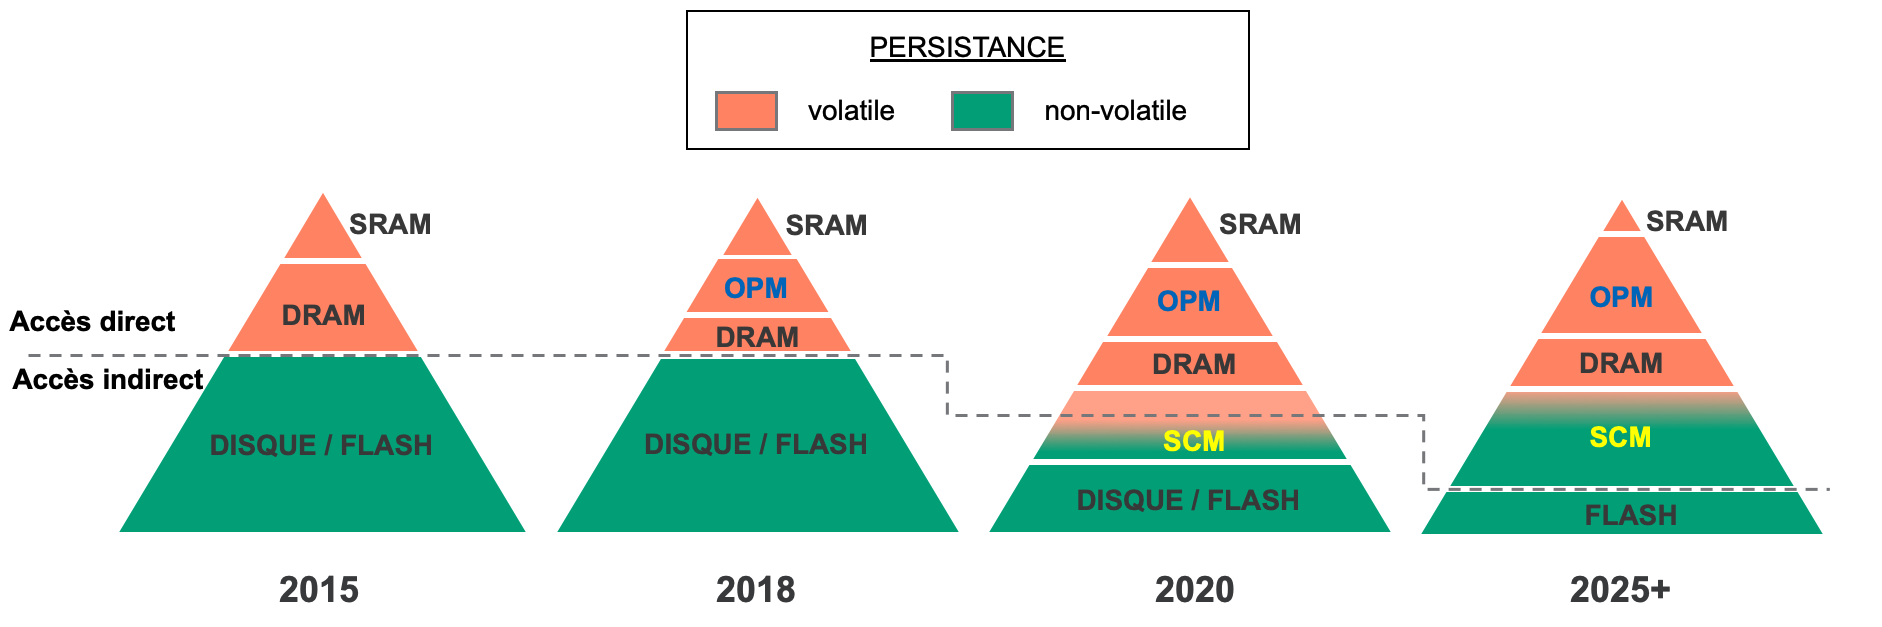
\includegraphics[width=17cm]{images/edl_scm_evo.png}
        \caption{\label{fig:edl_scm_evo} Évolution du système mémoire: les mémoires OPM (On Package Memory) telles que la HBM et les mémoires SCM (Storage Class Memory) vont permettre de compléter les trous de performance respectifs entre la SRAM et la DRAM ainsi qu'entre la DRAM et la mémoire flash.}
        \end{figure}
        
        
        \begin{table}[]
        \centering
        \resizebox{\textwidth}{!}{%
        \begin{tabular}{|l|c|c|c|c|c|c|c|c|}
        \hline
        \textbf{Technologies} & \textbf{DDR} & \textbf{NAND} & \textbf{3DXP PCM} & \textbf{MRAM} & \textbf{STT-RAM} & \textbf{FeRAM} & \textbf{RRAM} & \textbf{NRAM} \\ \hline
        \textbf{Persistance} & \cellcolor[HTML]{FD6864}Non & Oui & Oui & Oui & Oui & Oui & Oui & \cellcolor[HTML]{67FD9A}Oui \\ \hline
        \textbf{Endurance} & \cellcolor[HTML]{67FD9A}$10^{15}$ & \cellcolor[HTML]{FD6864}$10^{3}$-$10^{5}$ & \cellcolor[HTML]{FD6864}$10^{6}$ & $10^{12}$ & \cellcolor[HTML]{67FD9A}$10^{15}$ & \cellcolor[HTML]{67FD9A}$10^{14}$ & \cellcolor[HTML]{FD6864}$10^{6}$ & \cellcolor[HTML]{67FD9A}$10^{15}$ \\ \hline
        \textbf{Latence R/W} & \cellcolor[HTML]{67FD9A}10ns/10ns & 50us/25us & \cellcolor[HTML]{FD6864}100ns/1us & 50ns/1us & 50ns/100ns & 50ns/50ns & \cellcolor[HTML]{FD6864}200ns/1us & \cellcolor[HTML]{67FD9A}10ns/10ns \\ \hline
        \textbf{Énergie (pJ)} & \cellcolor[HTML]{67FD9A}0.005 & \cellcolor[HTML]{FD6864}1360 & \cellcolor[HTML]{FFCC67}150 & 2 & 1 & 0.3 & \cellcolor[HTML]{FFCC67}64 & \cellcolor[HTML]{67FD9A}.005 \\ \hline
        \textbf{Densité} & moyenne & \cellcolor[HTML]{67FD9A}haute & moyenne & faible & faible & faible & moyenne & moyenne \\ \hline
        \textbf{Rétention} & \cellcolor[HTML]{FD6864}4us & 1 an & 10 ans & \cellcolor[HTML]{FFCC67}jours & \cellcolor[HTML]{FFCC67}jours & 10 ans & 10 ans & \cellcolor[HTML]{67FD9A}10 ans \\ \hline
        \textbf{Adressabilité} & byte & \cellcolor[HTML]{FD6864}Page & byte & byte & byte & byte & byte & byte \\ \hline
        \textbf{Scalabilité} & 16nm & \cellcolor[HTML]{67FD9A}QLC, 96L+ & \textless{}20nm & 28nm & 28nm & \cellcolor[HTML]{FD6864}40nm & \textless{}20nm & \cellcolor[HTML]{67FD9A}\textless{}10nm \\ \hline
        \textbf{Price /GB} & \cellcolor[HTML]{FFCC67}7\$ & \cellcolor[HTML]{67FD9A}\textless{}1\$ & 3.5\$ & \cellcolor[HTML]{FD6864}2K\$ & \cellcolor[HTML]{FD6864}4K\$ & \cellcolor[HTML]{FD6864}32K\$ & 3.5\$ & \cellcolor[HTML]{FFCC67}6\$ \\ \hline
        \textbf{Status} & Prod. & Prod. & Prod. & Prod. & Prod. & \cellcolor[HTML]{FFCC67}Prod. / fin & \cellcolor[HTML]{FD6864}échantillon & \cellcolor[HTML]{FD6864}échantillon \\ \hline
        \end{tabular}%
        }
        \caption{État de l'art des différentes technologies SCM comparées à la DRAM et à la mémoire flash.}
        \label{tab:SCM}
        \end{table}
        
        Le développement de ces technologies n'est pas récent. On retrouve par exemple un article sur le développement de \textbf{mémoire PCM} (mémoire à changement de phase) daté de 1969 \cite{Sie1969}. C'est notamment la technologie utilisée pour les mémoires XPoint d'Intel \cite{Handy2015}. Elle utilise certaines propriétés des matériaux chalcogénures tels que la photosensibilité ou la résistivité électrique. Ces matériaux subissent une transition de phase sous l'effet de la température. Cette transition de phase modifie leur conductivité ce qui permet d'encoder l'information. Le matériau peut être chauffé de deux façons: à l'aide d'un laser (utilisé pour les disques optiques réinscriptibles (CD-RW)) ou en utilisant l'effet joule. La lecture se fait ensuite en mesurant sa résistance à l'aide d'un courant suffisamment faible pour ne pas modifier son état. Ces mémoires, insensibles aux radiations sont particulièrement intéressantes dans des conditions d'utilisation inhabituelles celles de l'aérospatiale. \textbf{La MRAM} (\textit{RAM magnétique}) utilise le spin des électrons.  Suivant leur orientation par rapport à un aimant, la résistance change et permet de stocker l'information. En 2003, IBM a produit le premier démonstrateur avec la production de la première mémoire MRAM de 128kb  \cite{Bette2003}. Depuis, d'autres constructeurs ont produit de telles mémoires comme Freescale (un million de puces vendues), Samsung et Hynix. Le futur de cette technologie est d'évoluer en STT-RAM \cite{Alvarez-Herault2010} (\textit{spin transfer torque} MRAM) permettant d'atteindre des densités d'intégrations plus élevées, une latence réduite proche de celle de la DRAM. Grâce à une consommation électrique faible, cette mémoire pourrait être adaptée pour les objets connectés (IOT). \textbf{La FeRAM} ou Mémoire Ferroélectrique à accès aléatoires possède la même structure que la DRAM avec un matériau ferroélectrique à la place du diélectrique. Cette technologie permettrait de profiter de la simplicité de la DRAM avec une intégration plus élevée (mais inférieure à celle de la mémoire flash \cite{Alvarez-Herault2010}). Beaucoup de problèmes sont rencontrés dans leur fabrication, notamment la pollution du silicium par le PZT. \textbf{La NRAM} (Nano RAM) repose sur l'utilisation de nanotubes de carbone. Un réseau de tubes croisés est activé électrostatiquement à l'aide d'une différence de potentiel pour faire fléchir les tubes et les mettre en contacte ou non \cite{Ricart2008}. Ses performances proches de celles de la DRAM en font un excellent remplaçant. La production de mémoires utilisant cette technologie est relativement simple et plusieurs couches peuvent être empilées pour augmenter la densité \cite{Gervasi2019}. \textbf{La ReRAM} (RAM résistive) se base sur le déplacement de trous dans des cristaux dopés. La production de cette mémoire est relativement simple et permettrait d'obtenir des prix compétitifs. Le désavantage de cette mémoire est la faible endurance aux écritures proche de celui de la flash. Le développement de cette technologie n'est pas encore terminé, et n'aboutirait pas avant 2025.
        
        

%\newpage


\subsection{Nouvelles technologies d'interconnexion.}
%%%%%%%%%%%%%%%%%%%%%%%%%%%%%%%%%%%%%%%%%%%%%%%%%%    

    Dans la section précédente, nous avons discuté du besoin de développer de nouvelles technologies mémoire. Cependant, pour pouvoir profiter de débits plus élevés que ceux atteints actuellement, il est indispensable de développer de nouvelles technologies pour améliorer la performance du bus mémoire et du système d'interconnexion. Dans cette section, nous étudions les débits du bus mémoire et la consommation énergétique du système d'interconnexion des plateformes actuelles. Nous présentons ensuite de nouvelles technologies pouvant être utilisées. 

    \subsubsection{Débit mémoire des processeurs} 
        
        Nous proposons d'étudier l'utilisation d'un processeur Intel Skylake pour l'exécution d'applications HPC typiques. Un tel processeur possédant 28 coeurs cadencés à 2.3 GHz, réalise en performance crête 2 TFLOPS (voir détail du calcul dans la \autoref{sec:methodo_step1}). En supposant l'utilisation d'un bus mémoire délivrant 100 Gb/s, nous calculons le débit de donnée transférable pour chaque opération exécutée:
        \begin{equation}
            \frac{100 \times 10^9 \; byte/s}{2 \times 10^{12} \; FLOP/s} = 0.05 \; byte/FLOP
        \end{equation}
        Ce résultat signifie que pendant l'exécution d'une opération, le système mémoire est capable de transférer 0.05 byte de la mémoire au processeur. Les applications de simulation numérique, telles que celles utilisées dans le domaine de la recherche pétrolière basée sur des algorithmes de Stencil, ont besoin de transférer depuis la mémoire 2 bytes par FLOP (4 pour l'application HPCG\footnote{Report on the HPC application bottlenecks - \url{http://exanode.eu/wp-content/uploads/2017/04/D2.5.pdf}}), l'idéal se trouvant autour des 8 bytes par opération \cite{Bergman2015}. Cette valeur est estimée pour un algorithme utilisant parfaitement la localité des mémoires cache et utilisant des opérations en double précision. On remarque donc que le système mémoire est très loin d'être capable de délivrer suffisamment de données pour permettre au processeur d'atteindre sa puissance crête (facteur 40). 
        
    %%%%%%%%%%%%%%%%%%%%%%%%%%%%%%%%%%%%%%%%%%%%%%%%%%%%%%%%%%%%%%%
    
    \subsubsection{Consommation du système d'interconnexion} 
        
        Les applications de calculs parallèles doivent échanger certains résultats entre serveurs. Il est courant d'utiliser des valeurs entre $0.1$ et $0.2 \; byte/FLOP$ \cite{Bergman2015} pour des applications de simulation numérique. Pour pouvoir fournir suffisamment de données aux serveurs, la plateforme exascale devrait utiliser un système d'interconnexion avec un débit équivalent à:
        \begin{equation}
            0.2 \; byte/FLOP \times 10^{18} \; FLOP/s = 200 \times 10^{15} \; byte/s
        \end{equation}
        Les plateformes du Top500 allouent autour de 15\% de leur budget énergétique total \cite{bergman2008exascale}, pour l'alimentation du système d'interconnexion. Pour une plateforme Exascale consommant 20 MW cela correspond à une enveloppe énergétique de 3 MW. Nous pouvons ainsi calculer le budget d'énergie utilisable pour le transfert de chaque donnée:
        \begin{equation}
            \frac{3 * 10^6 \; joule/s}{200 * 10^{15} \; byte/s} = 15 \; pJ/byte = 1.87 \; pJ/bit
        \end{equation}
        Cette énergie représente l'enveloppe énergétique totale utilisable pour transférer un bit d'informations entre deux noeuds du système. Ce transfert comprend le passage dans les différents commutateurs. Or, comme nous l'avons expliqué dans la \autoref{sec:edl_chal_energie}, le budget actuellement nécessaire pour un tel transfert dépassait 1000 pJ/bit.
    
    %%%%%%%%%%%%%%%%%%%%%%%%%%%%%%%%%%%%%%%%%%%%%%%%%%%%%%%%%%%%%%%
    
    \subsubsection{Objectifs des nouvelles technologies d'interconnexion} 
        
        Nous constatons donc le besoin de nouvelles technologies d'interconnexion. La diminution de la consommation énergétique de trois ordres de grandeur ne pourra pas provenir d'une simple évolution des technologies actuellement utilisées:
        \begin{itemize}
            \item \textbf{La consommation électrique} doit être réduite de plusieurs facteurs, non seulement pour le système d'interconnexion, mais aussi pour les accès mémoires. La programmation d'algorithmes efficaces (localité) est alors primordiale. 
            \item \textbf{Les débits mémoires} offerts doivent être améliorés de plusieurs facteurs pour pouvoir alimenter les processeurs et les accélérateurs. 
            \item \textbf{La latence} du système d'interconnexion devra être la plus faible possible pour permettre à certaines applications de générer des accès mémoire imprédictibles (parcours de graphes). Les jeux de données ne pouvant pas être stockés sur une seule machine, le système d'interconnexion doit posséder une latence très faible pour pouvoir accéder rapidement à une donnée distante.
        \end{itemize}
        Afin de répondre aux défis exposés précédemment, l'industrie du HPC s'est lancée depuis plusieurs dizaines d'années dans la recherche et le développement de technologies photoniques. 
    
    %%%%%%%%%%%%%%%%%%%%%%%%%%%%%%%%%%%%%%%%%%%%%%%%%%%%%%%%%%%%%%%%%%%%%%%
    
    \subsubsection{La photonique}
    
        La photonique est un domaine de la physique qui a pour objectif de manipuler la lumière (photon): l'émission, la transmission, la captation et le traitement. Les premiers émetteurs ont été développés dans les années 1960. Aujourd'hui, la photonique a de nombreuses applications: lecteur de code-barre et DVD, illumination LED, vision nocturne\ldots Dans le domaine des télécommunications, l'application la plus connue est la fibre optique. L'utilisation de technologies photoniques dans les supercalculateurs a deux avantages principaux répondant aux besoins évoqués ci-dessus.
       
        \begin{itemize}
            \item \textbf{L'indépendance à la distance} est le premier avantage de la photonique. Que ce soit en termes de latence ou de consommation électrique, la photonique permet de \textit{réduire les distances} d'un supercalculateur. En effet, la génération d'un signal optique ou électronique nécessite une quantité d'énergie similaire. Cependant, pour les technologies photoniques, celle-ci évolue faiblement avec la distance de communication (\autoref{fig:edl_photo_pj}). Lorsque les accès sont proches (sur la puce), il n'y a pas d'avantages en terme énergétique à utiliser la technologie photonique. Cependant, une fois les photons générés, le coût énergétique ne varie que faiblement avec la distance d'accès, et cela jusqu'à plusieurs centaines de mètres. Ainsi, le coût énergétique d'un accès mémoire est proche de celui d'un accès à une mémoire distante située sur un autre serveur. Pour ces accès, la photonique permet de réduire la consommation électrique de plusieurs ordres de grandeur. 
    
            \item \textbf{Les débits mémoire}s atteignables par l'utilisation de la photonique sont le deuxième avantage. À la différence des signaux électriques qui interfèrent lorsqu’ils sont utilisés sur une même broche, il est possible d’accumuler plusieurs signaux de différentes longueurs d’onde sur le même guide d’onde (\textit{wave guide}). Il est ainsi possible d'atteindre une haute densité de communication (voir \autoref{fig:edl_photo_bw}). Ces technologies peuvent atteindre des débits de 800 Gb/s avec une consommation de 2.2 pJ/bit. Les prochaines générations permettront d'atteindre des débits de 1 Tb/s  avec une consommation de 1 pJ/bit \cite{Bergman2018}. Cette faible densité va permettre d'utiliser la photonique à l'intérieur des puces permettant d'atteindre des débits élevés pour par exemple connecter une mémoire HBM au processeur.
        \end{itemize}
        
        
        \begin{figure}[t!]
            \centering
            \begin{subfigure}[t]{0.48\textwidth}
                \centering
                \includegraphics[width=\linewidth]{images/edl_photo_pj.png}
                \caption{\label{fig:edl_photo_pj} Distance d'accès et consommation électrique. } 
            \end{subfigure}\hfill
            \begin{subfigure}[t]{0.48\textwidth}
                \centering
                \includegraphics[width=\linewidth]{images/edl_photo_bw.png}
                \caption{\label{fig:edl_photo_bw} Distance d'accès et débit mémoire.}
            \end{subfigure}
            \caption{\label{fig:edl_photo} La transmission par photonique a deux avantages principaux comparés à la transmission électronique\cite{Lucas2014}: diminution de la consommation électrique (a) et amélioration du débit (b).}
        \end{figure}
    
    
        % Nouveaux usages
        L'utilisation des technologies photoniques dans les supercalculateurs va permettre de \textit{réduire} les distances en améliorant les latences de communication ainsi qu'en réduisant les coûts énergétiques. Il sera donc presque équivalent de communiquer avec sa propre mémoire, qu'avec celle d'un serveur situé à l'autre bout du centre de données. Ainsi, les supercalculateurs utilisés par plusieurs utilisateurs subiront moins les effets de fragmentation, car il n'y aura plus d'inconvénient à utiliser des machines distantes. Cependant, la topologie des calculateurs va devoir être repensée pour exploiter cette caractéristique (voir \autoref{sec:gen_z}).
        
        
        %ANNEAUX 
        De nombreuses technologies sont développées pour rendre possible l'utilisation de la photonique dans les centres de données. Par exemple, en utilisant des anneaux résonnants directement sur les puces silicium (voir \autoref{fig:edl_photo_ring_prez}). Ces anneaux sont des guides d’onde bouclés, permettant, pour une longueur d'onde donnée, de générer une résonance et propager l'onde dans celui-ci. Pour pouvoir contrôler les signaux, différents types d'anneaux ont été développés (voir \autoref{fig:edl_photo_ring}). Chaque anneau a une fonctionnalité permettant de réaliser différentes opérations: laisser passer ou non un signal, le commuter ou encore détecter la présence d'une certaine longueur d'onde. D'autres types d'anneaux sont utilisés pour générer les signaux et permettent d'encoder les informations à transmettre. En combinant ces anneaux, il est possible de développer des composants complexes comme des commutateurs.
        
        \begin{figure}[t!]
            \centering
            \begin{subfigure}[t]{0.48\textwidth}
                \centering
                \includegraphics[width=\linewidth]{images/edl_photo_ring1.png}
                \caption{\label{fig:edl_photo_ring1} Anneau résonnant vu au microscope.}
            \end{subfigure}\hfill
            \begin{subfigure}[t]{0.40\textwidth}
                \centering
                \includegraphics[width=\linewidth]{images/edl_photo_ring2.png}
                \caption{\label{fig:edl_photo_ring2} Fonctionnement d'un anneau résonnant}
            \end{subfigure}
            \caption{\label{fig:edl_photo_ring_prez} Illustration d'un anneau résonnant}
        \end{figure}
        
        \begin{figure}
            \center
            \includegraphics[width=14cm]{images/edl_photo_ring.png}
            \caption{\label{fig:edl_photo_ring} Différents types de résonateur en anneau.}
        \end{figure}


\subsection{Nouvelles architectures}\label{sec:new_soc}
%%%%%%%%%%%%%%%%%%%%%%%%%%%%%%%%%%%%%%%%%%%%%%%%%%%
    
    Dans cette section nous présentons les nouvelles architectures et les méthodes employées pour améliorer les performances des processeurs et des accélérateurs utilisés dans les supercalculateurs. Pour cela nous présentons la méthode de \textit{co-design} et présentons quelques architectures novatrices. Enfin, nous  discutons de la nécessité d'avoir des architectures hétérogènes pour atteindre l'efficience énergétique espérée.
    
    \subsubsection{Codesign}\label{sec:codesign}
        
        En informatique, le co-design (ou co-conception) est un processus de conception de système informatique impliquant différents acteurs: fabricant, programmeurs, utilisateurs finaux. Ce processus a pour objectif d'influencer la conception des architectures et le développement de technologies en tenant compte des besoins logiciels et algorithmiques. Il regroupe autour de partenariat longue durée l'expertise des fournisseurs, des architectes, des scientifiques et des programmeurs dans le but de développer les meilleures technologies possibles en fonction des besoins exprimés (coût, performance, efficacité énergétique). Le co-design est une piste majeure pour le développement de processeurs et d'accélérateurs ultras optimisés utilisés dans l'élaboration de plateformes \gls{exascale}. La motivation principale étant de réfléchir à la façon de développer une plateforme exascale répondant aux besoins des applications plutôt que de se demander quelles applications sont adaptées à cette plateforme une fois celle-ci développée \cite{PARKERe2013}.
        
        \begin{figure}
        \center
        \includegraphics[width=14cm]{images/edl_co_design.png}
        \caption{\label{fig:edl_co_design} Processus de co-design.}
        \end{figure}
        
        Le développement en co-design suit un processus d'aller-retour entre la partie logicielle et la partie matérielle (voir \autoref{fig:edl_co_design}). Les utilisateurs de HPC (programmeurs, scientifiques) expriment les besoins de leurs applications aux constructeurs de matériels: débit mémoire, latence, scalabilité, puissance de calcul. Cette étape peut être difficile, car certaines applications comptent plusieurs millions de lignes de codes, et l'expression de leurs besoins est loin d'être triviale. Il peut alors être intéressant d'utiliser des applications plus simples se comportant comme les applications réelles (benchmarks, micro-benchmarks). 
        En étant conscient des besoins des applications, les fabricants peuvent développer des architectures adaptées. Pour cela, il est nécessaire d'utiliser toutes les avancées technologiques réalisées dans différents domaines (mémoire, interconnexion). Ensuite, les constructeurs peuvent communiquer aux développeurs certaines spécificités du matériel qui peuvent être exploitées par le logiciel (caractéristiques de la hiérarchie mémoire, instructions utilisables). Le principal frein de cette méthode est économique. Il faut que l'utilisation d'une architecture puisse bénéficier au maximum d'applications pour qu'un constructeur prenne la décision de la développer.
        
        Ces solutions pourront être développées pour accélérer certains algorithmes ou motifs de calcul \cite{asanovic2006landscape}: algèbre linéaire (matrices creuses ou denses), méthode spectrale (transformation de Fourier rapide), algorithmes de Monte-Carlo, graphe, programmation dynamique. Un exemple de co-design vise à adapter les unités de calcul aux besoins des applications (instructions vectorielles, précision). Lorsque celles-ci ne nécessitent pas de réaliser des calculs avec une grande précision, il peut alors être intéressant d’utiliser des registres plus petits. L’étude \cite{Horowitz2014} montre que les opérations flottantes sur des registres plus petits consomment moins d’énergie: 0.03 pJ pour une addition sur 8 bits contre 0.9 pJ pour une addition sur 32 bits. De plus, le coût énergétique d’une multiplication évolue avec la taille ($n$) des registres utilisés ($O(n^2)$) ainsi que la latence ($O(n)$) \cite{Sze2017}. Enfin, le nombre de transistors nécessaires est réduit avec la taille des registres ($36 \mu m^2$ contre $4184 \mu m^2$) pour des additionneurs de 8 et 32 bits \cite{Horowitz2014}. Cette technique a été utilisée par Google pour le développement de son ASIC en 2015. Le TPU est un ASIC optimisé pour réaliser la phase d'inférence des modèles d'apprentissage. Cette phase ne nécessite pas d'avoir autant de précision que la phase d'entraînement. Les ingénieurs ont donc développé le TPU en utilisant 65536 registres de 8 bits. Cette réduction d'un facteur 8 permet de réduire la consommation électrique et la taille des circuits par un facteur 6 \cite{Jouppi2017}. La latence de réponse, importante pour la phase d'inférence, est réduite entre 15 et 30 fois par rapport au GPU équivalent de l'époque (Nvidia K80).
            
          
            
            %Les architectures pourront ensuite être utilisées dans d'autres systèmes (ordinateurs personnels, téléphones). Ces méthodes sont déjà largement utilisées dans le domaine de la programmation embarquée, qui utilisent des processeurs (ou ASIC) prévus pour des tâches spécifiques. 
    
        %%%%%%%%%%%%%%%%%%%%%%%%%%%%%%%%%%%%%%%%%%%%%%%%%%%
        
    \subsubsection{Quelques nouvelles architectures}\label{sec:new_arch}
    
        Pour répondre aux défis exposés dans la section précédente, de nombreuses entreprises se lancent dans le développement de nouvelles architectures, qui peuvent être très différentes de celles que nous utilisons depuis 30 ans. En janvier 2018, une étude \cite{Metz2018} a dénombré 45 start-ups qui développaient des circuits spécialisés pour certaines applications d’intelligence artificielle: analyse de voix, conduite autonome\ldots Cinq  d’entre elles avaient alors levé plus de 100 millions de dollars d’investissement. Les derniers classements du Top500 ont vu l'apparition de supercalculateurs utilisant de nouveaux accélérateurs ou l'évolution d'anciennes architectures. Par exemple, les GPU Nvidia utilisaient seulement de la mémoire GDDR5 sur les cartes des architectures Keppler. La génération suivante (Volta) a permis d'utiliser un interposeur en silicium connectant directement au processeur une mémoire HBM2. Ceci a permis de réduire les coûts énergétiques associés aux communications de 100 pJ/bit à moins de 10 pJ/bit. L'efficacité énergétique des supercalculateurs a ainsi pu être améliorée, passante de 6,7 à 14,1 GFLOPS/watt\footnotetext{Comparaison des classements du Top500 entre juin 2016 et 2017 des supercalculateurs Shoubu et Tsubame3.0}. En plus de nouvelles cartes GPU (Nvidia V100), deux nouveaux accélérateurs sont utilisés dans les supercalculateurs classés en tête du Green500: le PEZY-SC2 et le processeur ARM A64FX. Nous comparons les principales caractéristiques de ces architectures avec celle d'un processeur Intel moderne (génération Kaby Lake) dans le \autoref{tab:new_soc}.
        
                
        % Please add the following required packages to your document preamble:
        % \usepackage{graphicx}
        \begin{table}
        \centering
        \resizebox{\textwidth}{!}{%
        \begin{tabular}{|l|c|c|c|c|c|c|}
        \hline
         & \textbf{Coeurs/Thread} & \textbf{Freq. (GHz)} & \textbf{Débit mémoire (GB/s)} & \textbf{Perf. DP (TFLOPS)} & \textbf{TDP (Watt)} & \textbf{Eff. (GFLOPS/watt)} \\ \hline
        Intel Xeon 6246 & 12 / 24 & 3.30 & 140 (DRAM) & 1 & 165 & 6 \\ \hline
        Nvidia V100 & 5120 & 1.5 & 900 (HBM2) & 7.8 & 300 & 26 \\ \hline
        Pezy-SC2.2 & 2048 / 16384 & 1 & 2000 (DRAM + HBM2) & 4.1 & 180 & 23 \\ \hline
        Fujitsu A64FX & 48 & Non communiquée & 1000 (HBM2) & 2.7 & 180 & 15 \\ \hline
        \end{tabular}%
        }
        \caption{Caractéristiques et performances d'architectures utilisées dans les supercalculateurs les plus efficaces du Top500.}
        \label{tab:new_soc}
        \end{table}
                
        \textbf{Les architectures PEZY-SCx} sont des accélérateurs multicoeurs développés par la société PEZY.  Ils sont utilisés dans plusieurs supercalculateurs (ZettaScaler) construits au Japon. La dernière version, PEZY-SC2, a une surface six fois plus grande que le processeur Intel auquel il est généralement associé. La puce dispose de quatre canaux mémoires permettant d'atteindre une bande passante de 95.37 GB/s. En plus, l'accélérateur utilise une technologie sans fil (ThruChip Interface (TCI)) pour communiquer avec une mémoire 3D (voir \autoref{fig:edl_pezy_arch}). Chaque interface peut atteindre 500 GB/s pour un total de 2 TB/s. 
          
        \begin{figure}[t!]
            \centering
            \begin{subfigure}[t]{0.48\textwidth}
                \centering
                \includegraphics[width=\linewidth]{images/edl_pezy_arch.png}
                \caption{\label{fig:edl_pezy_arch}microarchitecture de l'accélérateur.}
            \end{subfigure}\hfill
            \begin{subfigure}[t]{0.48\textwidth}
                \centering
                \includegraphics[width=\linewidth]{images/edl_pezzy_board.png}
                \caption{\label{fig:edl_pezzy_board}Plusieurs PEZY-SC2 peuvent être connectés sur un serveur.}
            \end{subfigure}
            \caption{\label{fig:pezy} Accélérateur PEZY-SC2 \cite{RyutaroHimenoToshikazuEbisuzaki2018}}
        \end{figure}
        
        \textbf{Le processeur ARM A64FX} développé par Fujitsu est le processeur équipant le premier supercalculateur classé au Green500. Il possède 48 coeurs capables d'exécuter des instructions vectorielles de 512 bits. Il est doté de 32 GB de mémoire HBM2 permettant d'atteindre la performance de 2.7 TFLOPS ($10^{12}$ \gls{FLOPS}). Alors que le processeur A64FX n'est pas le plus efficace des 4 processeurs listés dans le \autoref{tab:new_soc}, il est pourtant utilisé dans le premier supercalculateur du Green500. En effet, nous remarquons que la puissance électrique d'une architecture ne suffit pas à déterminer l'efficacité énergétique d'une solution complète. Le reste de la plateforme doit lui aussi rentrer en compte (mémoire, utilisation du port PCI-E). La densité d'installation des architectures peut aussi avoir un impact (voir \autoref{fig:edl_pezzy_board}). Ainsi, bien que le GPU Nvidia V100 soit le plus efficace, ce sont les solutions utilisant les processeurs ARM et PEZZY qui sont les mieux classées.
        
    \subsubsection{Hétérogénéité} \label{sec:edl_hpc_hetero}
        
        Avec la fin de la validité de la loi de Dennard et les premiers signes d'apparition du ``mur'' de l'énergie, les constructeurs ont été contraints de repenser la microarchitecture des processeurs. Les processeurs utilisés étaient alors désignés comme d'usage général (\textit{general purpose processor} (GPP)). Permettant d'exécuter tout type d'application, ces processeurs ne sont optimisés pour aucune d'entre elles. 
        La performance et l'efficacité énergétique sont les deux raisons qui ont poussé la communauté HPC à adopter cette technologie. L'évolution des langages et des libraires a permis de faciliter les développements d'application pour ces accélérateurs. En 2007, Nvidia publiait CUDA, un langage propriétaire permettant de programmer les cartes graphiques de la marque ainsi que des librairies de calculs mathématiques optimisées (CUBLAS, CUFFT). Ainsi, le nombre de supercalculateurs hétérogènes présents dans le Top500 n'a fait qu'augmenter ces dix dernières années pour atteindre près d'un supercalculateur sur trois en 2019 (voir \autoref{fig:edl_hetero_share}). À partir de 2010, les premiers clusters contenant des cartes graphiques apparaissent au classement du Top500 (voir le graphique \ref{fig:edl_gpu_top500}). Il faut attendre 2011 pour voir une réelle percée de cette technologie. En 2018, les GPUs étaient les principaux accélérateurs utilisés dans les supercalculateurs (93\% des plateformes hétérogènes du Top500 en 2018). 
        
        
        

       \begin{figure}[t!]
            \centering
            \begin{subfigure}[t]{0.58\textwidth}
                \centering
                \includegraphics[width=\linewidth]{images/edl_gpu_top500.png}
                \caption{\label{fig:edl_gpu_top500} Évolution des différents types d'accélérateurs utilisés \cite{Strohmaier2018}.}
            \end{subfigure}\hfill
            \begin{subfigure}[t]{0.41\textwidth}
                \centering
                \includegraphics[width=\linewidth]{images/edl_hetero_share.png}
                \caption{\label{fig:edl_hetero_share} Évolution du pourcentage de supercalculateurs utilisant un accélérateur \cite{phdthesis}.}
            \end{subfigure}
            \caption{Évolution de l'utilisation d'accélérateurs dans les supercalculateurs.}
        \end{figure}
        
        
        En 2020, la majorité des supercalculateurs n'utilise cependant pas d'accélérateurs. En effet, les plateformes homogènes ont plusieurs avantages. La performance des processeurs GPP peut être suffisante pour une majorité d'applications. L'utilisation d'une seule famille de processeur facilite aussi la gestion du centre de calculs. Aussi, l'utilisation d'un processeur type x86 assure une stabilité à long terme, où l'utilisation de la génération suivante d'une architecture est similaire et ne nécessite généralement pas de grosse transformation de code. 
        
        D'un autre coté, utiliser des architectures hétérogènes peut présenter plusieurs difficultés. La première vient de la nécessité de transformer ou de reprogrammer les applications pouvant nécéssiter l'utilisation de langages  ou des modèles de programmation différents. Ces transformations demandent un gros investissement des programmeurs. D'autres difficultés concernent la gestion et l'utilisation des ressources. Les supercalculateurs sont utilisés pour exécuter différents types d'applications, avec différents besoins. Utiliser un seul type d'accélérateur ne sera pas efficace pour toutes les applications. Le nombre de combinaisons engendrées par la disponibilité de plusieurs types d'accélérateurs, de capacité de mémoire différente complique l'obtention des performances optimales. La recherche des configurations optimales (compilateur, drapeaux de compilation, type d'accélérateur, taille de découpage des jeux de données, nombre de coeurs et fréquence utilisés) est alors difficile à réaliser manuellement. Pour explorer les différentes configurations, il peut alors être intéressant de se tourner vers des techniques d'autoréglage (\textit{auto-tuning}) \cite{datta2008stencil, hoste2008cole, mazouz2011performance, castro2015cere, popov:tel-01412638,  benkner_et_al:DR:2014:4423} 
        
        Une récente étude \cite{inproceedingsSCHC} conduite auprès de plusieurs industries montre que l'investissement nécessaire pour réaliser ces transformations est un frein majeur à l'adoption de ces architectures. La transformation du code est loin d'être évidente et varie en fonction des accélérateurs choisis (voir \autoref{fig:edl_many_techno}). Les langages, librairies et outils de programmation (déboguer, suivi de performance) sont moins avancés et moins robustes que ceux utilisés sur des architectures classiques. Les quatre entreprises interviewées \cite{inproceedingsSCHC} constatent le manque d'outils adaptés pour réaliser le travail du portage de code et de validation de performances. C'est une différence majeure entre l'industrie et le domaine de la recherche. Les applications industrielles sont plus complexes que celles utilisées comme démonstrateurs et il est souvent plus difficile d'atteindre les performances théoriques. Une entreprise témoignant dans l'étude \cite{inproceedingsSCHC} affirme que le manque d'expertise était le principal défi pour le portage d'application. Ce constat est partagé par les autres entreprises présentées comme grandes (\textit{large}) et ayant les moyens d'embaucher de potentiels experts.
        
        Cependant, les pressions énergétiques et économiques obligeront les plus grands centres à se doter de plateformes hétérogènes malgré les difficultés associées. 
        
        \begin{figure}
        \center
        \includegraphics[width=17cm]{images/edl_many_techno.png}
        \caption{\label{fig:edl_many_techno} Différentes technologies sont disponibles, chacune ayant ses avantages et inconvénients.}
        \end{figure}
            
        Dans le projet \gls{exascale}, l'hétérogénéité ne viendra pas seulement de l'utilisation d'accélérateurs différents. Les architectures elles-mêmes seront développées à partir de différentes technologies, pour maximiser l'efficacité énergétique. Le co-design associé aux technologies photoniques va permettre le développement d'architectures ultra-optimisées permettant la construction d'une plateforme \gls{exascale} consommant entre 20 et 30 MW. Les puces des processeurs vont être adaptées à l'application pour minimiser les échanges de données (voir \autoref{fig:edl_hetero_chip}). Un même processeur pourra alors disposer de différents types de coeurs (complexes (x86), simples (GPU), programmables (FPGA)) ayant des mémoires aux caractéristiques, elles aussi différentes (capacité, latence, débit, politique de remplacement, associativité).  Par exemple, une application d'apprentissage automatique peut avoir besoin pendant la phase d'entraînement de ressources similaires aux GPU. Dans une seconde phase (inférence), un autre module (FPGA, ASIC), directement accessible sur la puce, peut alors être utilisé. Ainsi, les données ne nécessitent par d’être transférées sur un autre serveur et peuvent être encore présentes dans la hiérarchie mémoire (mémoire 3D, SCM, DRAM).
        
          \begin{figure}
        \center
        \includegraphics[width=9cm]{images/edl_hetero_chip.png}
        \caption{\label{fig:edl_hetero_chip}Développement de processeurs très hétérogènes possédant différentes technologies sur la même puce et communiquant par photonique \cite{Bergman2018}.}
        \end{figure}
            
      

      
%%%%%%%%%%%%%%%%%%%%%%%%%%%%%%%%%%%%%%%%%%%%%%%%%%%%%%%%%%%%%%%%%%%%%%%%%%%%%%%%%%%%%%%%%%%%%%%%%%%%%%%%%%%%%%%%%%%%%
%%%%%%%%%%%%%%%%%%%%%%%%%%%%%%%%%%%%%%%%%%%%%%%%%%%%%%%%%%%%%%%%%%%%%%%%%%%%%%%%%%%%%%%%%%%%%%%%%%%%%%%%%%%%%%%%%%%%%
%%%%%%%%%%%%%%%%%%%%%%%%%%%%%%%%%%%%%%%%%%%%%%%%%%%%%%%%%%%%%%%%%%%%%%%%%%%%%%%%%%%%%%%%%%%%%%%%%%%%%%%%%%%%%%%%%%%%%
%%%%%%%%%%%%%%%%%%%%%%%%%%%%%%%%%%%%%%%%%%%%%%%%%%%%%%%%%%%%%%%%%%%%%%%%%%%%%%%%%%%%%%%%%%%%%%%%%%%%%%%%%%%%%%%%%%%%%
%%%%%%%%%%%%%%%%%%%%%%%%%%%%%%%%%%%%%%%%%%%%%%%%%%%%%%%%%%%%%%%%%%%%%%%%%%%%%%%%%%%%%%%%%%%%%%%%%%%%%%%%%%%%%%%%%%%%%


\subsection{Gen-Z}\label{sec:gen_z}
%%%%%%%%%%%%%%%%%%%%%%%%%%%%%%%%%%%%%%%%%%%%%%%%%%
    
    Cette section est consacrée à la présentation d'un nouveau protocole de communication nommé Gen-Z. Pour cela, nous résumons les principales motivations de la nécessité d'utiliser une telle technologie. Nous présentons ensuite les principales caractéristiques et les avantages du protocole. Enfin, nous discutons de l'opportunité apportée par Gen-Z pour repenser fondamentalement l'architecture de nos plateformes.
        
    \subsubsection{Motivations}
            %%%%%%%%%%%%%%%%%%%%%%%%%%%%%%%%%%%%%%%%%%%%%%%%%%%%%%%%%%%%%%

        % EXPLOSION
        Le tsunami de données générées présenté dans la \autoref{sec:challenges} nécessite de repenser la façon dont nous les traitons. Actuellement ces données sont envoyées aux centres de calculs pour être analysées. Le volume de données générées dans les prochaines années nous empêchera de poursuivre cette méthode. Une voiture connectée génère par exemple entre 2 et 5 terabytes de données chaque jour. Le coût des technologies et des infrastructures nécessaires pour les transférer vers les centres de données serait alors trop élevé. De plus, la conduite autonome comme d'autres applications (villes connectées) nécessite d'avoir des réponses rapides. La seule solution viable est alors de les traiter le plus proche possible de leur zone de création. Seule une partie d'entre elles sera alors remontée aux centres de calculs pour l'archivage ou améliorer l'apprentissage des réseaux de neurones.
        
        %securité
        Les voitures et les objets connectés produisent des données sensibles, et la nécessité d'utiliser des plateformes de traitement sécurisées est primordiale. Chaque composant des solutions est une source d’attaque potentielle: capteurs, processeurs, mémoires, réseaux. Les dégâts potentiels d'une attaque sur ces sites ultra-connectés pourraient alors être catastrophiques (attaque de la signalisation routière, de voitures connectées ou d'un système de refroidissement d'une centrale nucléaire).
    
        % HETERO
        Concernant le domaine du HPC, nous avons expliqué dans les sections précédentes que de nombreuses technologies (mémoires, processeurs, accélérateurs) étaient en développement. Ces nouvelles architectures sont produites par différents constructeurs. De plus, les architectures actuelles ont été développées pour un nombre limité de technologies (mémoire DRAM, processeur x86 ou ARM, extension PCIe). Ainsi, la principale difficulté pour leur utilisation viendra de leur inter-compatibilité. 
        
       
                
    \subsubsection{Limites des architectures actuelles}
        %%%%%%%%%%%%%%%%%%%%%%%%%%%%%%%%%%%%%%%%%%%%%%%%%%%%%%%%%%%%%%
        Malgré l'évolution des accélérateurs et l'utilisation de nouvelles technologies mémoire, les architectures actuelles ne pourront pas évoluer indéfiniment et ont déjà montré leurs limites. La \autoref{fig:edl_genz_evo_memoire}, représente l'évolution des différentes caractéristiques liées aux bus de communication d'un processeur ainsi que l'évolution du nombre de coeurs disponibles. Nous constatons que l'évolution du nombre de coeurs a évolué plus rapidement que celle des performances du système mémoire. En effet, lorsque le nombre de canaux mémoires a été multiplié par 2 (passant de 4 à 6, puis à 8 canaux) le nombre de coeurs a été multiplié par un facteur 8.  Le débit du bus mémoire (courbe violette) et du bus PCIe (courbe rouge) disponible par coeur a donc diminué. La majorité des broches du processeur est déjà utilisée par les canaux mémoires et il sera très difficile d'en allouer plus. 
        
            \begin{figure}
            \center
            \includegraphics[width=14cm]{images/edl_genz_evo_memoire.png}
            \caption{\label{fig:edl_genz_evo_memoire} Évolution annuelle des caractéristiques principales des architectures (nombre de coeur, débit mémoire) et leur impact sur les débits disponibles par coeur.}
            \end{figure}
            
        
        %PLace
        De plus, le manque d'espace disponible sur la carte mère nous oblige à développer une solution permettant d'augmenter les débits de plusieurs facteurs avec les canaux actuellement utilisés. 
        L'espace disponible autour du processeur pour ajouter des emplacements mémoires est aussi de plus en plus limité. Les plus grosses configurations actuelles peuvent atteindre jusqu'à 1.5 TB de mémoire, insuffisant pour traiter les jeux de données envisagés.
    
        % lock step &
        Avec le modèle actuel, l'évolution des mémoires ou des processeurs est verrouillée. La nécessité que l'un soit compatible avec l'autre oblige les deux parties à évoluer de manière synchronisée. Par exemple, avant de pouvoir utiliser des mémoires DDR5, il faut que les processeurs les supportant soient développés. Cette dépendance est un frein à l'évolution.
        
        %SCM
        Le développement des mémoires SCM permettra à terme d'obtenir des performances proches de la DRAM. Cependant, elles ne permettront pas d'augmenter les débits mémoires de plusieurs facteurs. En effet, ces mémoires sont installées sous forme de barrettes mémoire (NVDIMM voir \autoref{sec:nvdimm}) ou sous forme d'extensions de carte PCI (comme les mémoires Intel Optane). Que ce soit sous forme de barrette ou de carte PCI, la restriction de performance vient du bus utilisé. De plus, l'utilisation d'extension PCI a ses limites, car ce bus ne supporte pas la cohérence de cache des mémoires associées (contrairement au bus mémoire).

        %Protocol Babel
        Un autre défaut des architectures actuelles impactant la performance des applications concerne la multiplicité des protocoles utilisés: DDR, PCIe, infiniband, Ethernet, sata (voir \autoref{fig:edl_genz_babel}). L'utilisation de différents protocoles à un coût, impactant la latence, le débit et l'énergie consommée pour chaque transfert. Pour développer une plateforme exascale efficace, il est donc nécessaire de revoir l'utilisation de ces protocoles.
            
           
        
   
        %%%%%%%%%%%%%%%%%%%%%%%%%%%%%%%%%%%%%%%%%%%%%%%%%%%%%%%%%%%%%%
        %%%%%%%%%%% GEN _ Z %%%%%%%%%
        %%%%%%%%%%%%%%%%%%%%%%%%%%%%%%%%%%%%%%%%%%%%%%%%%%%%%%%%%%%%%%
    
    \subsubsection{Gen-Z.}
        
    % DEFINITION
        Gen-Z est un protocole universel d'interconnexion, de puce à puce, permettant les échanges entre composants informatiques au travers de communications à sémantique en mémoire. Gen-Z est dit universel, car il permet de connecter différentes architectures (CPU, GPU, FPGA) ainsi que différents médias (mémoire, stockage, archive) à travers un unique protocole (voir \autoref{fig:edl_genz_overview}). Ces communications (asynchrones) peuvent être locales (entre les composants d'un même serveur), ou bien externes (entre deux serveurs). 


       \begin{figure}[t!]
            \centering
            \begin{subfigure}[t]{0.49\textwidth}
                \centering
                \includegraphics[width=\linewidth]{images/edl_genz_babel.png}
                \caption{\label{fig:edl_genz_babel} De nombreux protocoles sont impliqués lors d'une communication.}
            \end{subfigure}\hfill
            \begin{subfigure}[t]{0.49\textwidth}
                \centering
                \includegraphics[width=\linewidth]{images/edl_genz_overview.png}
                \caption{\label{fig:edl_genz_overview} Le protocole Gen-Z permet d'interconnecter tous les composants d'une plateforme.}
            \end{subfigure}
            \caption{\label{fig:edl_genz_babel_topo} Gen-Z permet d'utiliser un unique protocole pour la totalité des communications.}
        \end{figure}
        
        
        Lancé en 2016, il est développé par un consortium qui compte aujourd'hui plus de 70 membres\footnotetext{Liste des membres du consortium Gen-Z - \url{https://genzconsortium.org/about-us/membership/members/}}, dont les plus grandes entreprises du domaine informatique: AMD, ARM, Cisco, Dell, Google, HP, HPE, Micron, Microsoft, Redhat, Samsung\ldots Il est important de noter l'absence de deux constructeurs majeurs (Intel et Nvidia) qui ont rejoint un deuxième consortium pour le développement d'un second protocole nommé CXL\footnotetext{Compute Express Link - \url{https://www.computeexpresslink.org/}}. Le développement de CXL est moins avancé que celui de Gen-Z.
        
        Ce protocole a été développé pour répondre aux nombreux défis posés par l'utilisation des objets connectés et la nécessité de traiter des grands jeux de données. Gen-Z permet d'adresser un espace mémoire $2^{92}$ Byte (soit 4096 yottabytes, soit mille fois plus grands que notre espace numérique actuel) et d’interconnecter 16 millions d'objets. Ces objets pouvant être des composants d'un serveur (mémoire, processeur, accélérateurs) ou des objets connectés plus complexes.
            
    
    % SEMANTIQUE MEMOIRE

        \paragraph{Sémantique mémoire.} 
            L'avantage de Gen-Z est d'utiliser des communications à sémantique mémoire. Tous les composants sont considérés comme des modules mémoires et peuvent être accédés grâce à des instructions \textit{load/store}. Il est ainsi possible d'adresser les mémoires SCM par byte et non plus par bloc (héritage dû aux disques optiques). En réduisant la complexité des instructions, le processeur et le système d'exploitation ne sont pas impliqués dans leur exécution, libérant des ressources pour l'exécution d'autres instructions. Gen-Z propose d'autres instructions permettant de réaliser des opérations plus complexes telles que les opérations atomiques (comparaison, addition), des interruptions ou encore de gérer la cohérence des caches.
        
            Comme exposé en présentation de cette section, les évolutions technologiques des différentes parties d'une architecture sont dépendantes les unes des autres. Gen-Z permet de supprimer ce verrou. La \autoref{fig:edl_genz_bus_evo} présente comment les processeurs et les mémoires vont utiliser les interfaces Gen-Z pour être indépendantes. Le processeur et la mémoire auront une interface Gen-Z et l'évolution d'une partie ne nécessitera pas de changement de l'autre. De plus, en spécifiant un protocole universel, Gen-Z assure l'interopérabilité entre tout type de composant qui possède une interface (CPU, FPGA, GPU, DSP, I/O, mémoires).

            \begin{figure}[t!]
                \centering
                \begin{subfigure}[t]{0.49\textwidth}
                    \centering
                    \includegraphics[width=\linewidth]{images/edl_genz_current_bus.png}
                    \caption{\label{fig:edl_genz_current_bus} Actuellement les technologies mémoire et celles des processeurs sont liées.}
                \end{subfigure}\hfill
                \begin{subfigure}[t]{0.49\textwidth}
                    \centering
                    \includegraphics[width=\linewidth]{images/edl_genz_new_bus.png}
                    \caption{\label{fig:edl_genz_new_bus} Avec Gen-Z, chaque module aura sa propre interface.}
                \end{subfigure}
                \caption{\label{fig:edl_genz_bus_evo} Déverrouiller l'évolution technologique grâce à Gen-Z.}
            \end{figure}


    \paragraph{Latence et débit.}

        %Latence
        Le protocole Gen-Z permet d'améliorer les performances du système d'interconnexion et apporte aussi de nouvelles fonctionnalités permettant de repenser l'architecture des plateformes. La réduction du nombre de protocoles et des différentes couches impliquées dans le transfert des données (système de fichier, tampon I/O, drivers) permet de réduire les latences des accès. Les spécifications actuelles permettraient de réduire le nombre d'instructions de 25000 à 3 pour réaliser un transfert d'une donnée localisée sur un disque. En utilisant des technologies SCM, les latences d'accès entre un processeur et une mémoire située sur un autre serveur seraient alors proches de celles d'un accès à la mémoire DRAM locale (inférieur à 250 ns).
     
        %BANDE PASSANTE    
        Gen-Z permet d'atteindre des débits mémoires supérieurs à ceux des bus mémoires actuels. En fonction des technologies et du nombre de broches utilisées, les débits mémoires d'une architecture Gen-Z peuvent atteindre 1.7 TB/s. Ces performances sont possibles grâce au débit atteignable pour chaque broche du processeur utilisée. Il sera donc possible d'atteindre des débits mémoires 10 fois supérieurs avec seulement la moitié de broches. Ceci permettra de développer des processeurs moins coûteux.
        % À titre de comparaison, la mémoire DDR5 permet d'atteindre 0.55 GB/s par broche.
        
            
            
            

    \paragraph{Topologie}

        Gen-Z supporte nativement différentes topologies (P2P, mesh, Torus) pour réaliser la connexion entre les composants, mais aussi entre les serveurs (voir \autoref{fig:edl_genz_topo}). Ces topologies permettent d'implémenter des réseaux multi chemins (\textit{multipath}) et de gérer le contrôle de congestion. Si un lien entre deux composants est cassé, le protocole s'adapte automatiquement en passant par d'autres chemins disponibles. Les différents composants peuvent alors servir de relais pour transmettre les paquets. Aujourd'hui lorsqu'un serveur tombe en panne, les données présentes dessus sont perdues, et les applications doivent être relancées. Gen-Z et les SCM permettront d'assurer une connexion permanente aux différents modules avec l'utilisation de la topologie HyperX \cite{Ahn2009} (voir \autoref{fig:edl_photo_hyperX}),  qui permet de joindre n'importe quel serveur avec trois routes différentes. Cette redondance permet d'éviter les congestions et d'assurer une utilisation maximale du supercalculateur même en cas de panne d'une des connexions.
             
        \begin{figure}
            \center
            \includegraphics[width=14cm]{images/edl_photo_hyperX.png}
            \caption{\label{fig:edl_photo_hyperX} La topologie HyperX permet de joindre n'importe quel serveur grâce à trois routes différentes.}
        \end{figure} 
            
            %Module mémoire
                \begin{figure}
                \center
                \includegraphics[width=14cm]{images/edl_genz_topo.png}
                \caption{\label{fig:edl_genz_topo} Le protocole Gen-Z permet d'implémenter nativement différentes topologies.}
            \end{figure}
            
            

    \paragraph{Sécurité}

        La sécurité est un aspect fondamental du développement de Gen-Z. La sécurisation des échanges est en effet très importante si ce protocole doit être utilisé à l'extérieur des centres de calculs. Chaque composant Gen-Z est identifié lors de leur création en usine. Il est ainsi possible d'authentifier n'importe quelle transaction. Le protocole peut ainsi permettre à un routeur de bloquer ou non une communication. La sécurité est réalisée par un logiciel centralisé et assurée physiquement par chaque matériel grâce à l’utilisation de clefs d’accès. Les accès interdits sont rapportés au gestionnaire pour éventuellement déceler des attaques. De nombreux mécanismes de sécurité sont développés contre les attaques de type \textit{man-in-the-middle}, comme l'utilisation de tags \textit{anti-replay} \cite{Radhakishan2011}.

    \subsubsection{Nouvelles plateformes} \label{sec:oppo_new_tech} \label{sec:compute_on_the_edge}
            
        Associé aux technologies présentées précédemment comme les mémoires non volatiles (SCM) et/ou les technologies d'interconnexion rapides à faible consommation (photoniques), Gen-Z va permettre de repenser l'architecture des plateformes. Le calcul piloté par la mémoire (Memory Driven Computing (architecture MDC)) désigne une nouvelle façon d'organiser les architectures en plaçant la mémoire au centre (voir \autoref{fig:edl_mdc}). L'architecture MDC donne à chaque processeur l'accès à un grand espace de mémoire partagée (\textit{memory pool}) (\autoref{fig:edl_mdc_new}). C'est la différence majeure avec les architectures actuelles où chaque processeur possède son propre espace mémoire local (\autoref{fig:edl_mdc_old}). L'avantage de cette architecture est de pouvoir combiner différents éléments de calcul (processeur, accélérateurs) autour de ces espaces mémoire. En fonction des besoins des applications, différentes plateformes peuvent être développées pour répondre précisément au besoin.
    
            \begin{figure}[t!]
                \centering
                \begin{subfigure}[t]{0.49\textwidth}
                    \centering
                    \includegraphics[width=\linewidth]{images/edl_mdc_old.png}
                    \caption{\label{fig:edl_mdc_old} Plateformes actuelles}
                \end{subfigure}\hfill
                \begin{subfigure}[t]{0.49\textwidth}
                    \centering
                    \includegraphics[width=\linewidth]{images/edl_mdc_new.png}
                    \caption{\label{fig:edl_mdc_new}Plateforme MDC}
                \end{subfigure}
                \caption{\label{fig:edl_mdc} Les plateformes MDC inversent l'architecture en plaçant la mémoire au centre.}
            \end{figure}

        %MEMORY
        Les trois principales caractéristiques dont vont bénéficier les applications sont: le \textit{partage} d'un \textit{grand espace} de mémoire \textit{persistant}. 
        Tous les serveurs partageant le même espace mémoire, il n'est plus nécessaire de réaliser des communications explicites pour échanger des données. Pour le programmeur, cela implique de ne plus avoir à se soucier de partitionner et répartir les jeux de données entre chaque serveur. 
        L'utilisation de \textbf{grands espaces mémoire} permet de repenser certains algorithmes. Par exemple en précalculant des graphes pour optimiser leur parcours, ou explorer simultanément plusieurs alternatives. En fonction des motifs d'accès mémoires réalisés, plusieurs versions d'un même jeu de données peuvent être utilisées permettant de profiter des techniques de localités.
        La totalité des jeux de données pouvant être stockée en \textbf{mémoires persistantes}, il n'est plus nécessaire de réaliser des sauvegardes régulières des données sur des périphériques de stockage beaucoup plus lents.

        %MEMORY POOL
        Un même module mémoire pourra être fragmenté et utilisé par différentes ressources. Grâce à Gen-Z, il est possible d'assigner dynamiquement une zone mémoire à une ressource même si celle-ci ne se trouve pas sur le même serveur.  Associé à des technologies comme la photonique, l'accès à ces mémoire pourra être très rapide, permettant de créer des espaces mémoire distants de grande capacité. Une zone mémoire peut alors être partagée entre différentes ressources travaillant sur un même jeu de données, ou pour réaliser des communications en mémoire (synchronisation). Lorsqu'un accélérateur doit communiquer des résultats à un second accélérateur, il lui suffit de lui autoriser l'accès à cette zone mémoire et lui transmettre un pointeur associé.
           
         %Superdome
         HPE développe depuis plusieurs années une architecture MDC connue sous le nom de code de \textit{The Machine}. Ce projet a donné lieu à la première gamme de serveurs MDC: HPE Superdome Flex. Ces plateformes peuvent embarquer 32 processeurs partageant 48 TB de mémoire. Les premiers résultats ont montré l'énorme saut de performance pouvant être atteint pour certaines applications. Une application de calcul de graphe \cite{Chen2016a} a ainsi pu être accélérée d'un facteur 128 en utilisant une plateforme de 12 TB de mémoire. HPE utilise des simulateurs permettant de prédire les gains de performances qu'un algorithme peut potentiellement atteindre. Les résultats de ces simulations ont montré que certaines applications utilisées dans le domaine de la finance (simulation Monte-Carlo) pourraient être accélérées d'un facteur 10 000.
   
               
      \begin{figure}
        \center
        \includegraphics[width=14cm]{images/edl_superdome.png}
        \caption{\label{fig:edl_superdome}Les serveurs HPE Superdome possèdent un espace mémoire \textit{attaché} partagé entre les différents processeurs.}
        \end{figure}

\section{Caractérisation et analyse de performance des architectures}
\label{chap:performance} \label{sec:edl_perf_intro}

    Dans la section précédente, nous avons discuté des différentes opportunités disponibles pour permettre la construction de plateformes \gls{exascale}. De nouvelles technologies comme les mémoires SCM ou la photonique vont permettre de développer de nouvelles architectures. Grâce au protocole Gen-Z, différentes architectures pourront facilement être interconnectées dans une même plateforme. L'efficacité énergétique étant primordiale, il est fondamental de trouver les architectures les plus adaptées pour chaque application et d'optimiser leur code pour en tirer la performance maximale. Nous proposons ainsi d'étudier deux domaines permettant de réaliser ce travail: le domaine de la caractérisation d'architecture et le domaine du suivi de performance. 
    
    La \autoref{sec:caracterisation} présente les méthodes et les outils existants permettant de caractériser les matériels. Dans un supercalculateur, de nombreuses ressources doivent être caractérisées: le processeur, le système d'interconnexion, le système de stockage... 
    Dans ce travail de thèse, nous nous sommes principalement intéressés à la caractérisation de la microarchitecture des processeurs et du système mémoire:
    \begin{itemize}
        \item Les applications \gls{hpc} utilisent ces architectures pour exécuter des opérations sur des nombres à virgule flottante (\gls{FLOP}). Nous nous intéressons donc au matériel responsable de leur exécution: les unités arithmétiques et logiques (ALU).
        
        \item La performance de la majorité des applications étant limitée par le système mémoire, nous nous intéresserons dans un second temps à la caractérisation du système mémoire. Ce dernier étant composé d'une hiérarchie de différentes mémoires, il est important de pouvoir caractériser ses différents niveaux: taille, latence, débit.
    \end{itemize}
    
    La \autoref{sec:profiling} présente les méthodes et les outils existants permettant de suivre les performances des applications. La complexité des architectures et la différence d'évolution des performances du système mémoire et des processeurs empêchent les applications d'atteindre les performances maximales délivrées par les processeurs. 
    \begin{itemize}
        \item Le temps d'exécution des applications HPC est généralement passé dans une faible portion des lignes de codes. Ces zones, appelées \glspl{hotspot}, doivent être identifiées pour être caractérisées et optimisées. Pour cela, le programmeur doit utiliser des outils permettant d'obtenir les profils de performances d'une application et identifier ces zones de codes.
        
        \item Il est ensuite nécessaire de pouvoir mesurer la performance effective de ces zones de code. Lorsque la performance maximale n'est pas atteinte, il est alors nécessaire de pouvoir en expliquer les raisons. 
    \end{itemize}
    
      
\subsection{Caractérisation des architectures}\label{sec:caracterisation}
%%%%%%%%%%%%%%%%%%%%%%%%%%%%%%%%%%%%%%%%%%%%%%%%%%%%%%%%%%%%%%%%%%%%%%%%
%%%%%%%%%%%%%%%%%%%%%%%%%%%%%%%%%%%%%%%%%%%%%%%%%%%%%%%%%%%%%%%%%%%%%%%%
    
    Dans cette partie, nous présentons les différentes méthodes permettant de caractériser les architectures. Nous utilisons le terme \textit{caractérisation} pour désigner la capacité à identifier les forces et les faiblesses d'une architecture ainsi que d'en mesurer certaines caractéristiques. Afin de choisir la meilleure architecture pour une application il est nécessaire de connaître ces différentes caractéristiques: capacité de calcul, performance mémoire (débit, latence)...
    
    Il existe deux façons de caractériser une architecture: 
    \begin{itemize}
        \item La première consiste à utiliser les données communiquées par le constructeur d'une plateforme pour calculer la performance du matériel. Dans la \autoref{sec:methodo_step1} nous montrons comment le débit mémoire et la performance de calcul théoriques peuvent être calculés à partir des documentations techniques. Cette approche est intéressante, car elle permet de caractériser une architecture sans y avoir accès. Cependant, certaines données peuvent ne pas être disponibles et nécessitent d'avoir accès aux architectures pour les obtenir. Des outils disponibles sur les distributions Linux (\textit{lscpu\footnote{\url{http://man7.org/linux/man-pages/man1/lscpu.1.html}}, cpumap\footnote{\url{https://www.plafrim.fr/fr/outils-sgi/}}, cpuid\footnote{\url{https://www.felixcloutier.com/x86/cpuid}}}) peuvent alors être utilisées pour les obtenir. Néanmoins, ces outils peuvent ne pas supporter toutes les architectures et certaines données peuvent manquer.
    
        \item La seconde méthode nécessite d'avoir accès à l'architecture dans le but d'y exécuter des codes dont l'objectif est de mesurer la performance. Ces codes, appelés \glspl{benchmark}, sont présentés dans la section suivante. Contrairement à la première méthode, l'utilisation de ces applicatifs permet de mesurer une performance réellement atteignable (performance crête). En effet, il est rare que la performance mesurée soit égale à la performance théorique calculée à partir des données techniques de l'architecture. Le développement de nouvelles architectures, et la complexité de leur microarchitecture peuvent donner lieu à des bogues et conduire à de mauvaises performances. Il est donc important de les caractériser pour identifier une erreur, mais aussi pour comparer la performance d'une application avec la performance réelle de l'architecture.
    \end{itemize}
    
           
    \subsubsection{Benchmarks}
    %%%%%%%%%%%%%%%%%%%%%%%%%%%%%%%%%
           
        En informatique, un \gls{benchmark} est un code, ou un ensemble de codes, permettant de mesurer la performance d'une solution et d'en vérifier ses fonctionnalités. Lors de la phase de conception d'une architecture, des benchmarks peuvent être utilisés pour détecter la présence de bogues ou pour valider certaines fonctionnalités. Cela permet d'estimer la performance d'un matériel avant qu'il ne soit produit (grâce à des simulateurs par exemple). Les codes de benchmark sont pour la majorité en version libre de droits. Cela permet leur large utilisation et permet de comparer la performance de différentes plateformes (le classement du Top500 est réalisé grâce au benchmark HPL). En informatique, nous pouvons classer les benchmarks selon quatre catégories \cite{Staelin2004}:
        
        \begin{enumerate}

            \item  \textbf{Les benchmarks} sont des applications complètes exécutant différents types d'instructions: calculs, transferts mémoires, réseaux... Il peut aussi arriver que des applications réelles soient finalement utilisées comme programme de benchmark tel que BSMBench \cite{HPC:bsmbench} utilisé pour réaliser des motifs de calculs similaires à ceux réalisées en théorie de jauge (physique des particules). \textbf{TODO reprendre}
        
            \item  \textbf{Les benchmarks noyaux} (\textit{kernel-based benchmark}) sont des codes simples permettant de caractériser une partie spécifique du matériel. Ces codes artificiels peuvent être de simples extraits de benchmark. Le benchmark noyaux STREAM \textbf{todo citation} consiste en l'exécution de quatre fonctions différentes qui à l'origine étaient utilisées pour étudier les différences de performances entre deux architectures pour exécuter des applications pour la modélisation du climat. Il est aujourd'hui utilisé pour mesurer le débit mémoire atteignable par un processeur.
        
            \item \textbf{Les micro benchmarks} sont des benchmarks noyaux permettant d’isoler une partie précise de l’architecture à évaluer. Par exemple, lmbench \cite{HPC:lmbench} est une suite de micro benchmarks portables utilisés pour mesurer des caractéristiques importantes de la mémoire telles que la bande passante, la latence mémoire et les performances des différents niveaux de cache.  Les informations récupérées permettent de mettre en oeuvre des optimisations en s'adaptant parfaitement aux caractéristiques d'une architecture.
      
            \item \textbf{Les générateurs de benchmarks} permettent de produire une application à partir d'un premier code. La génération a l'avantage de faciliter le test de plusieurs configurations différentes en faisant varier les paramètres d'entrée, la taille des jeux de données, ou encore l'algorithme utilisé pour résoudre une tâche. Ainsi, le logiciel de GeneNetWeaver \cite{schaffter2011genenetweaver} peut être utilisé pour générer dynamiquement des modèles génétiques pouvant ensuite être utilisés comme benchmark. Des bibliothèques de calcul telles que ATLAS \cite{whaley1998automatically} et FFTW \cite{frigo1998fftw} génèrent des micro benchmarks pour caractériser l'architecture. ATLAS génère ainsi des dizaines de versions différentes d'un code de multiplication de matrices pour estimer la taille de bloc la plus efficace pour exploiter les caches.
        \end{enumerate}    
   
     
    \subsubsection{Benchmarks existants}
    %%%%%%%%%%%%%%%%%%%%%%%%%%%%%%%%%

        Comme indiqué dans l'introduction de cette section, nous nous sommes intéressés à la caractérisation du système mémoire ainsi qu'à celle des unités arithmétiques et logiques des processeurs. Ces unités sont responsables de l'exécution des instructions de calcul sur nombre à virgule flottante (FLOP). Elles sont donc un matériel essentiel des architectures pour l'exécution d'application de calcul intensif. Le système mémoire étant le goulot d'étranglement de la performance d'une majorité d'applications, de nombreux travaux ont été réalisés pour sa caractérisation et son optimisation. Dans cette partie nous énumérons et discutons les principaux benchmarks permettant de caractériser ces parties de l'architecture.


        %Il existe de nombreux benchmarks permettant de caractériser différentes parties du système mémoire: les accès mémoires concurrents de systèmes multiprocesseurs\cite{Mandal2010}, polices de mappage mémoire des systèmes NUMA \cite{Diener2015}, prédiction de la bande passante mémoire en fonction du placement des coeurs \cite{Wang2016a}, caractérisation de la hiérarchie mémoire \cite{Cooper2011}.
 
        

        \paragraph{HPL \cite{Dongarra2003}} 
            Un des micros benchmarks les plus utilisés est sans doute celui du HPL, utilisé pour construire le classement du Top500 \cite{HPC:top500}. Les premières versions du benchmark, alors appelé LINPACK, remontent aux années 1979 et permettaient d'estimer le temps de résolution d'un problème d'algèbre. Son utilisation comme benchmark est plus un accident qu'une réelle volonté. L'annexe B du manuel de l'utilisateur proposait aux utilisateurs d'estimer et de noter les temps de résolution en fonction de la machine utilisée. Pour pouvoir être utilisé sur les supercalculateurs, le benchmark a été parallélisé, changeant ainsi de nom en Highly Parallel Computing Benchmark, HPLinpack ou encore HPL. Il est utilisé pour mesurer le nombre maximum d'opérations à virgule flottante par seconde (\gls{FLOPS}) qu'un supercalculateur est capable de fournir pour la résolution d'un système linéaire d'équations utilisant la décomposition LU. Ainsi, avant d'être un benchmark de processeur, c'est un benchmark de librairie DGEMM (Intel MKL, netlib, GotoBLAS). La force de ce benchmark est de n'avoir qu'un résultat (soit la sommation des puissances de calculs de tous les coeurs utilisés). Il est donc très facile de comparer deux plateformes de calculs. Bien que mondialement utilisé, le HPL a un principal défaut qui est d'estimer la performance d'une plateforme en ne mesurant que sa capacité de calcul. Cependant, comme nous l'avons montré précédemment, la performance de la majorité des applications est limitée par la performance de la bande passante. La mesure du HPL n'est donc pas la plus représentative de la puissance d'un supercalculateur atteignable par des applications réelles. 
        
        \paragraph{HPCG \cite{Dongarra2013}} 
        \label{sec:hpcg}
            
            Admettant la faiblesse du benchmark HPL, son concepteur, Jack Dongarra, se mit à la recherche d'un ou d'un ensemble de benchmarks permettant de mieux caractériser ces plateformes. Avec Michael Heroux et Piotr Luszczek, ils ont présentèrent alors en 2015 le benchmark HPCG (high performance conjugate gradient). HPCG permet de couvrir de nombreux motifs de communication (globale et voisinage) et de calculs  (mis-à jour de vecteur, multiplication de matrices creuses). 
            Le premier prérequis était alors de pouvoir produire, grâce à ce nouveau benchmark, un classement des supercalculateurs représentatif de leur performance pour exécuter des applications réelles. Le deuxième prérequis fait suite à la crainte de voir la conception des processeurs être influencée pour obtenir de meilleures performances pour le benchmark HPL \cite{Dongarra2013}. Ainsi, HPCG utilise une mesure qui pousserait les concepteurs de processeurs à améliorer leurs matériels ce qui par conséquent profiterait aux applications réelles. \textbf{todo relire les temps de cette phrase avant} Là où HPL ne fournit qu'un seul résultat par exécution, HPCG en présente 128. Le classement du Top500 est aujourd'hui publié avec les valeurs obtenues par HPL et par HPCG\footnote{Classement HPCG 2019: \url{https://www.hpcg-benchmark.org/custom/index.html?lid=155&slid=302}}. Malgré la meilleure adéquation de HPCG à caractériser les plateformes, le benchmark HPL est, et sera probablement toujours utilisé, principalement pour des raisons d'historiques. En effet, il permet de suivre l'évolution des architectures depuis plus de 25 ans. 
            
        \paragraph{HPCC \cite{Luszczek2006}} 
            
            La suite de benchmark HPC Challenge vient compléter le benchmark HPL avec 6 codes dont certains réalisent des accès aux données permettant aussi de caractériser le système mémoire (voir \autoref{pic_bench_hpcc}). La suite de benchmarks est ainsi composée de HPL, Stream, DGEMM, RandomAccess, b\_eff, PTRANS, FFT. Avec l'ajout de ces six autres codes, la suite HPCC est plus représentative des applications réelles. Ces codes existaient avant la création de la suite HPCC. Le travail réalisé a permis de les regrouper dans une même suite, et de les améliorer avec des systèmes de vérifications et de rapport. Une fois compilé, un seul programme exécutable est généré permettant de faciliter son usage avec un gestionnaire de \textit{job}. Un seul exécutable étant généré, l'environnement d'exécution est le même pour tous les benchmarks de la suite (pas d'optimisation de pages larges pour un seul benchmark de la suite). 
            
            \begin{figure}
                \center
                \includegraphics[width=10cm]{images/bench_hpcc.png}
                \caption{ La suite de benchmark HPCC utilise des codes utilisant des localités différentes permettant de mieux caractériser les architectures
                \label{pic_bench_hpcc}}
            \end{figure}
        
        
        \paragraph{SPEC CPU2017 \cite{Bucek2018}} 
        
            Cette nouvelle génération de benchmark produite par SPEC (Standard Performance Evaluation Corporation) qui fait suite à la version précédente SPEC CPU2006. Ces deux initiatives ont permis de regrouper des applications réelles de tailles différentes, mais dont les performances sont limitées par la puissance de calcul de l'architecture. Les applications sélectionnées sont facilement portables. La première version contenait deux suites de benchmarks (CINT2006 \cite{Dilipbhai2012} et CFP2006 \cite{Sharkawi2009}) permettant de mesurer et comparer les performances de calculs en utilisant des opérations entières ou à nombres flottants. L'objectif principal de ces codes était alors de caractériser les performances du processeur, de la hiérarchie mémoire et du compilateur. La version 2017 possède 43 benchmarks qui sont portés sur plusieurs architectures dont AMD64, Intel IA32, Power ISA ou SPARC. Les benchmarks sont organisés en quatre suites permettant de mesurer le débit et la vitesse d'exécution d'opérations utilisant des nombres entiers ou flottants.  Les différents benchmarks ont un domaine d'application spécifique (compression vidéo, rendu 3D...) et peuvent être utilisés pour la conception de processeurs optimisés pour ces charges de travail \cite{Panda2018}. Malheureusement le prix de ces benchmarks avoisine les 1000\$. Cependant les nombreux résultats, libres de droits, sont publiés leur site internet. 
        
      %  \paragraph{SHOC \cite{danalis2010scalable}.} 
            %Les plateformes HPC modernes deviennent toujours plus hétérogènes avec l'utilisation d'accélérateurs comme les GPU ou les DSP. Suite à ce constat, la suite de benchmark Scalable HeterOgeneous Computing (SHOC) a été élaborée pour permettre l'évaluation de la performance et de la montée en charge de tels systèmes. La suite est composée de micro benchmarks et de benchmarks noyaux permettant d'évaluer précisément plusieurs architectures grâce à une implémentation MPI. Les codes utilise OpenCL et CUDA pour permettre une large utilisation. Une partie des codes est utilisée pour stresser l'architecture et identifier des problèmes matériels pouvant impacter la performance: mémoire défaillante ou un mauvais refroidissement. L'autre partie des codes est utilisée pour mesurer la performance de l'architecture grâce à des applications proches de celles utilisés en production. Le code source de la suite de benchmarks est disponible en ligne \footnote{\url{https://github.com/vetter/shoc/wiki}}.
       
        
     
        \paragraph{STREAM \cite{McCalpin1995}} 
        
        
            Le benchmark STREAM est sûrement un des benchmarks les plus connus et les plus utilisés au monde. Il a été développé et est maintenu par John McCalpin surnommé "Dr. Bandwidth". Le code STREAM permet de mesurer la bande passante mémoire atteignable grâce à l'implémentation de quatre noyaux: COPY ($c=a$), SCALE ($b=\alpha \times c$), ADD ($c=a+b$) et TRIAD ($a=b+\alpha \times c$). Les résultats sont donnés en GB/s et contiennent à la fois les opérations de lecture et d'écriture. Pour ces quatre opérations, STREAM fonctionne en générant un tableau de nombres aléatoires d'une taille spécifiée (qui est ensuite stocké en RAM) et effectue quatre types d'opérations: \textit{copy, scale, add, triad}.  Le benchmark utilise \textit{OpenMP} pour utiliser la totalité des coeurs disponibles. Ces différents tests étaient à l'origine destinés à caractériser la performance des architectures vectorielles. La performance mémoire pouvait alors varier d'une opération à l'autre. Aujourd'hui, la performance calculatoire des architectures n'est plus la contrainte principale et les quatre micro benchmarks obtiennent des performances équivalentes. Il est généralement accepté que la mesure donnée pour l'opération de \textit{triad} correspond à la bande passante maximale atteignable par l'architecture. On remarque que le noyau de calcul du \textit{triad} est relativement simple et ne consiste qu'en la lecture de deux éléments et l'écriture du résultat. Les applications réelles utilisant des motifs d'accès bien plus complexes, cette mesure n'est pas représentative de la performance réellement atteignable par celles-ci \footnote{\url{https://www.intel.ru/content/dam/doc/white-paper/resources-xeon-7500-measuring-memory-bandwidth-paper.pdf}}.
            
       
        \paragraph{Lmbench \cite{Staelin2004}} 
            
            %\textbf{Lire } biblio\_bench - lmbench an extensible micro-benchmark suite
            
            Le benchmark \textit{Lmbench}\cite{Staelin2004} a été développé par deux ingénieurs des HP Labs d'Israël en 2004. Ce code est en fait une suite de micro benchmarks permettant de mesurer la performance de plusieurs aspects d'une architecture: lecture d'un jeu de données, ouverture de fichiers, création de pipe, fréquence mémoire, taille d'une ligne de cache, taille de la TLB, bande passante mémoire (STREAM). L'ensemble des codes peut être exécuté pour caractériser la mémoire d'un système partagé ou distribué \cite{Staelin2002}.
            
            \textit{Lmbench} facilite l'ajout de nouveaux micro benchmarks et mesure leurs performances en donnant la latence par instruction et le débit mémoire. Le framework s'occupe de leur exécution pour atteindre des mesures de performances ayant une performance d'au moins 1\%. Écrit en ANSI-C et respectant la norme POSIX, le benchmark a été développé pour maximiser sa portabilité. Cependant, sa compilation sur des architectures récentes peut être plus difficile \cite{Yotov2004}. En raison de son incapacité à mesurer les performances du cache distant et les transactions de cohérence du cache, le benchmark \textit{x86-membench} benchmark \cite{Molka2017b} a été développé pour supporter la mesure de la bande passante et de la latence du cache local ou distant, mais aussi de la mémoire. Le benchmark n'utilise aucune méthode de parallélisme empêchant une caractérisation poussée des architectures modernes. 

        \paragraph{X-Ray \cite{Yotov2004}} 
        
           Pour aider les programmeurs à écrire de nouveaux benchmarks permettant de mesurer certains paramètres matériels l'outil X-Ray a été mis au point. X-Ray est un \gls{framework} permettant l'automatisation du développement de benchmarks. Pour cela il génère plusieurs benchmarks grâce à un framework \textit{Nano-benchmark Generator} (\autoref{pic_bench_xray}). Cette génération est dynamique, car les benchmarks à générer varient en fonction de ceux déjà exécutés. Si un benchmark a besoin de connaître la latence mémoire d'un niveau de cache, X-Ray exécutera alors le benchmark permettant de le calculer avant. X-Ray peut par exemple calculer la fréquence du processeur en ajoutant quatre nombres entiers avec des dépendances pour éviter les optimisations des processeurs superscalaires. Des benchmarks sont aussi disponibles pour caractériser la hiérarchie mémoire (associativité, taille des blocs, capacité, latence). Les résultats présentés sont annoncés plus précis que ceux donnés par les autres outils de l'état de l'art. Différents tests ont été réalisés sur des ordinateurs personnels, des serveurs ou encore des systèmes embarqués. Malheureusement le code n'est plus disponible pour être testé. 
            
            \begin{figure}
                \center
                \includegraphics[width=10cm]{images/bench_xray.png}
                \caption{ Structure d'un micro benchmark réalisé grâce à X-Ray  \cite{Yotov2004}.
                \label{pic_bench_xray}}
            \end{figure}
            
             Le travail \cite{Yotov2005} utilise X-Ray pour implémenter des micros benchmarks pour mesurer la capacité, l'associativité, la taille des blocs ainsi que la latence de chaque niveau de la hiérarchie de caches ainsi que du TLB. Contrairement aux benchmarks existants, l'outil mesure un niveau à la fois, lui permettant d'être plus précis que les approches traditionnelles (X-Ray, Calibrator, lmbench et MOB). Utiliser X-Ray pour implémenter leur benchmark leur permet de mesurer la fréquence du processeur ainsi que la latence et le débit des instructions. Malheureusement, le code de X-Ray n'a pas été maintenu et n'est plus disponible au téléchargement.
        
        \paragraph{P-Ray \cite{Duchateau2008}.} 
        
             
            Pour remédier à l'incapacité de \textit{lmbench} à caractériser les plateformes multicoeurs, le benchmark P-ray a été développé. Pour cela il étend les micros benchmarks existant pour trouver le niveau des caches partagé, la topologie d’interconnexion, la bande passante effective ou la taille des blocs pour la gestion de cohérence des caches. Pour éviter les optimisations du compilateur (\textit{pointer chaising}), le benchmark utilise un système de liste chaînée lors de l'initialisation. Les résultats obtenus sont eux très précis et s'approchent souvent des maximums théoriques attendus.

            Dans le but de permettre à certaines librairies (ATLAS, SPIRAL ou FFTW) de s'auto-optimiser, P-Ray permet de mesurer certains paramètres matériels. De la même façon que X-Ray et LMbench, l'apport de P-Ray permet de trouver ces spécifications pour des processeurs multicoeurs. P-Ray permet de décrire la répartition des caches entre les coeurs, la topologie d'interconnexion des processeurs ainsi que les mécanismes de cohérence de cache. Leurs expérimentations montrent des résultats très précis comme la mesure de la latence de communication entre deux coeurs à travers le cache L3 ou entre deux processeurs. Un effort particulier a été apporté pour éviter des optimisations du compilateur et du préchargment mémoire (\textit{memory prefetcher}) pouvant altérer les performances mesurées. Le benchmark P-Ray a hérité d'un problème de X-Ray rendant impossible la portabilité du code entre différents systèmes d'exploitation. L'allocation mémoire suppose que toutes les adresses physiques soient contiguës et cette caractéristique dépend du système d'exploitation (les pages larges pouvant ne pas être disponibles). Le code de P-Ray n'est cependant pas libre de droits.
        
        \paragraph{Servet \cite{gonzalez2010servet}.} 
            La suite Servet permet de mesurer certaines caractéristiques des matériels, telles que la hiérarchie de cache (taille, partage entre les coeurs) ou la bande passante mémoire. Ce travail complète X-Ray et P-Ray par des mesures de paramètres d'interconnexion pour la communication d'une mémoire distribuée ainsi qu'une méthodologie et une nouvelle technique de mesure \textbf{todo reprendre cette phrase}. Une suite de benchmarks permet aussi d'évaluer où se formeront les goulots d'étranglement lorsque plusieurs coeurs accèdent à la mémoire centrale. Enfin, Servet mesure la distance entre les coeurs en mesurant la latence de communication permettant à une application de placer plus efficacement les processus sur les différents coeurs.
               
        \paragraph{Saavedra \cite{Saavedra1995}} 
        
            Ce benchmark utilise une \gls{stride} (un saut en mémoire) de taille fixe pour accéder aux éléments d'un tableau. Le temps nécessaire à ces accès permet de déduire la taille des niveaux de la hiérarchie. Les expérimentations utilisent des couples de $\{taille de tableau, taille de stride\}$. La taille du tableau augmente jusqu'à atteindre la taille du cache mesuré. La taille des strides est limitée à des tailles de puissance de 2 et ne dépassera jamais la taille du cache. Le tableau est ainsi parcouru pendant au moins une seconde. Comme le souligne \cite{Yotov2005} le problème d'une telle approche est de vouloir mesurer tous les niveaux de la hiérarchie simultanément. Les mesures peuvent alors être influencées par différents paramètres de différents niveaux de caches. Ces mesures doivent être interprétées par l'utilisateur, le programme ne créant pas automatiquement la hiérarchie. La lecture et l'écriture sont réalisées sur la même donnée pouvant introduire des conflits dans le tampon d'écriture  \cite{Yotov2005}. Le benchmark suppose que les données sont continues en mémoire, mais n'utilise pas de pages larges.

       
\subsection{Analyse de performance d'une application}\label{sec:profiling}
%%%%%%%%%%%%%%%%%%%%%%%%%%%%%%%%%%%%%%%%%%%%%%%%%%%%%%%%%%%%%%%%%%%%%%%%
%%%%%%%%%%%%%%%%%%%%%%%%%%%%%%%%%%%%%%%%%%%%%%%%%%%%%%%%%%%%%%%%%%%%%%%%

        Le suivi de performances (\textit{performance monitoring}) a pour but de récolter des informations concernant une application ou concernant le système sur lequel elle est exécutée, pour la déboguer ou l'optimiser. L'analyse de performance peut être réalisée à différents niveaux \cite{imbert2011tips} : 
        \begin{itemize}
            \item Le premier niveau concerne l'utilisation d'un simulateur permettant d'étudier précisément (cycle par cycle) le comportement d'une architecture. Les données collectées peuvent être riches et permettent d'apporter des informations qu'il ne serait pas possible d'avoir avec l'exécution réelle de l'architecture. L'avantage de cette méthode est de pouvoir réaliser des premiers tests, sans avoir accès à l'architecture. Ces simulations peuvent modéliser la totalité de la microarchitecture et suivre l'exécution d'une application. Cependant, cette méthode nécessite le développement de simulateurs complexes que seul le constructeur peut développer. Les simulations précises (au cycle près) sont lentes (quelques centaines de cycles simulés par seconde) et génère de grandes quantités de données difficiles à analyser \cite{palomares2015combining}. Pour y remédier, des simulateurs plus simples utilisant des traces générées sur une architecture réelle peuvent être utilisés \cite{Cmelik1995}. Les traces sont collectées lors d'une première exécution sur une architecture et sont rejouées dans un simulateur pour être étudiées.
            
            \item Le second niveau correspond à l'analyse de la performance d'un serveur (coeur, processeur, système mémoire, réseaux). L'analyse de performance peut consister à vérifier la bonne répartition du travail entre les processeurs et la bonne utilisation des coeurs. Certains problèmes de performance peuvent venir de la mauvaise utilisation des mémoires caches ou de celle du bus mémoire. Au niveau le plus fin, l'analyse de la performance des coeurs peut être difficile, car elle nécessite l'utilisation d'outils précis. La complexité de la microarchitecture rend d'autant plus difficile cette analyse, de solides connaissances sont nécessaires pour pouvoir les analyser. Suite à cette analyse, diverses optimisations peuvent être nécessaires: préchargement de la mémoire, utilisation d'instructions vectorielles, amélioration de la gestion de la localité des données (\autoref{sec:locality})... Les informations utilisées pour l'analyse peuvent être obtenues en instrumentant le code (manuellement ou grâce au compilateur) ou en récupérant certaines informations de l'architecture (compteurs matériels).
            
            \item Le dernier niveau concerne l'analyse de la performance du supercalculateur complet. Il peut s'agir de vérifier la bonne utilisation de la programmation distribuée et la répartition du travail entre les noeuds. Les supercalculateurs \gls{exascale} devront être hétérogènes. Il est donc capital que l'ordonnanceur de tâche (\textit{job scheduler}) place efficacement les différents processus.
        
        \end{itemize}
        
        Pour parvenir à extraire la performance des supercalculateurs, l'analyse et l'optimisation des applications doivent être faites aux trois niveaux. Ce travail de thèse s'intéresse à l'analyse de performance du second niveau. Afin de permettre l'analyse, le portage et l'optimisation des codes, deux étapes principales sont étudiées:
        \begin{enumerate}
            
            \item \textbf{Identifier les hot spots.} En 1971, Donald Knuth affirmait que la majorité de l’exécution d'une application se déroulait dans une fraction des lignes de codes \cite{knuth1971empirical}. Cette affirmation est aussi connue sous le nom de principe de Pareto  (règle du 80/20). Ce principe empirique postule que 80\% des effets sont le produit de 20\% des causes. Dans le domaine de l’analyse de performance, cela signifie que 20\% des lignes de code sont responsable de 80\% du temps de l'exécution de l'application. Ces zones de codes sont appelées points chauds ou \glspl{hotspot}. Cela est d’autant plus vrai pour les applications de calcul haute performance où la proportion de code responsable d'une grande partie de la performance peut être encore plus faible. Il est facile de comprendre que c'est l'optimisation de ces zones de codes qui aura le plus d'impact sur l'amélioration de la performance de l'application. Il est donc nécessaire de pouvoir identifier et caractériser ces zones.
            
            \item \textbf{Identifier les goulots d'étranglement.} Une fois les zones de codes prenant une part majeure dans le temps d'exécution de l'application, il est nécessaire de quantifier leur performance pour trois raisons: 
            \begin{itemize}
                \item La première est de mesurer l'écart entre la performance réelle de l'application et la performance théorique atteignable par l'architecture pour quantifier les opportunités d'optimisations. 
                \item La deuxième est de pouvoir identifier les raisons et les parties de la microarchitecture qui sont responsables de cette performance. 
                \item La troisième est de permettre de caractériser leurs besoins: latence et débit mémoire, calcul, stockage...
            \end{itemize}
            Pour pouvoir comparer la différence entre la performance théorique et celle mesurée lors de l'exécution de l'application, il est courant d'utiliser des modèles de performances. Ces modèles prennent en compte les caractéristiques techniques d'une microarchitecture (FLOPS, débit mémoire...) ainsi que celles de l'application. L'utilisation de tels modèles permet ensuite de savoir quand le travail d'optimisation est terminé (performance maximale atteinte) ou de prédire la performance de la même application sur un système différent.
        \end{enumerate}
        
         Afin de répondre aux besoins exprimés ci-dessus, la suite de cette section présente les différentes méthodes et les outils existants qui permettent de suivre la performance d'une application. Nous présentons ensuite un modèle simple permettant de quantifier les performances mesurées d'une application.
           
      
 
    \subsubsection{Analyse statique et dynamique}
    %%%%%%%%%%%%%%%%%%%%%%%%%%%%%%%%%%%%%%%%%%%%%%%%%%%%%%%%%%%%%%%%%%%    
        
        Afin d'obtenir les informations nécessaires pour l'analyse de la performance d'une application, deux approches peuvent être employées: l'analyse statique et l'analyse dynamique.
        
        \paragraph{L'analyse statique}
            
            L’analyse statique consiste à obtenir des informations sur une application sans avoir à l'exécuter. Cette analyse peut permettre de détecter des bogues \cite{Lattner2016} ou de modéliser la performance de l'application grâce à l'utilisation de modèles analytiques. L'analyse peut être réalisée à partir du code source, ou des instructions assembleur générées par le compilateur \cite{Djoudi2005, wong2015vp3}. L'utilisation de l'assembleur permet de valider le bon fonctionnement du compilateur \cite{charif2014cqa}, mais rend plus difficile la corrélation avec le code source \cite{de2010new}.
            
            Des outils existent et permettent de réaliser des analyses statiques d'applications. 
            Intel propose différents outils tel que Intel Architecture Code Analyzer (IACA) \cite{Hirsh2012} qui permet de réaliser une analyse statique d'un code grâce à l'ajout de marqueur dans le code source. Il permet, pour un noyau identifié, de détecter la présence de dépendance entre plusieurs itérations de boucle et de donner une estimation des performances (débit d'instructions, saturation des ports de l'ALU...). Cependant, il est nécessaire d'avoir identifié les zones de \textit{hot spots} pour les annoter, et il ne fonctionne que pour des architectures Intel. Le projet a été abandonné en avril 2019\footnote{Intel IACA - \url{https://software.intel.com/en-us/articles/intel-architecture-code-analyzer}}.
        
            L’outil Modular Assembly Quality Analyzer and Optimizer (MAQAO) \cite{Djoudi2005} permet de désassembler un binaire pour en extraire le code assembleur et de lister les fonctions et les boucles importantes de l’application. Il peut ensuite faire un retour à l’utilisateur sur la qualité de son code et lui donner des conseils pour l’améliorer. Il permet d'analyser différents points, dont les 4 présentés dans \cite{popov:tel-01412638} :
            \begin{itemize}
                \item La pression appliquée par les instructions sur les différents ports du processeur pour en déterminer le bottleneck.
                \item La performance crête d'un code (qui suppose que toutes les données sont disponibles dans le premier niveau de cache).
                \item L’intensité arithmétique en mesurant le rapport du nombre d’instructions réalisant des opérations sur des nombres flottants et le nombre nombre total d’instructions à exécuter.
                \item Le ratio de vectorisation en mesurant le rapport du nombre d’instruction utilisant la vectorisation sur le nombre d’instructions pouvant potentiellement l’être.
            \end{itemize}
                      
            L'analyse statique ne nécessite pas l'exécution de l'application pour être réalisée. Ceci est très avantageux pour analyser les applications \gls{hpc} dont l'exécution peut durer plusieurs heures. Malheureusement, l'absence d'exécution ne permet pas de détecter les nombreux problèmes de performances dus à la complexité de l'architecture. Il est donc très difficile d'anticiper la performance réelle des applications. 
                 
        \paragraph{L'analyse dynamique}
            
            Contrairement à l'analyse statique, l'analyse dynamique nécessite l'exécution de l'application pour évaluer sa performance. Elle permet d’apporter de nombreuses informations impossibles à avoir grâce à l’analyse statique. Les informations peuvent être obtenues grâce à l'implémentation matérielle de registres permettant de suivre l'activité de la microarchitecture. Ces registres peuvent être simples (temps écoulé) ou complexes (nombre d'instructions vectorielles exécutées). Il y a deux façons d'utiliser ces compteurs: le comptage et l'échantillonnage.
               
            \begin{itemize}
                \item La première méthode consiste à \textbf{compter} le nombre d'évènements arrivant entre deux intervalles de temps. Pour cela, le compteur est initialisé à $0$ et lu au bout d'une certaine période de temps. Les valeurs ainsi récupérées permettent de mesurer le nombre d'occurrences de ces évènements. Cette méthode est efficace, mais elle ne permet pas de connaître la partie du code responsable d'un évènement. Les ratios d'évènements, tels que les instructions exécutées par cycle, les taux de \textit{miss} de mémoire cache et les taux d'erreurs de prévision des branches, peuvent être calculés en divisant le nombre par le temps écoulé.
                
                \item La deuxième méthode consiste à \textbf{échantillonner} ces informations. Ce mode consiste à déclencher une interruption tous les $n$ évènements et sauvegarder certaines informations telles que le pointeur d'instruction. Pour cela, le registre de comptage est initialisé à la valeur $\text{MAX} - n$ ou $\text{MAX}$ correspond à la valeur maximale pouvant être stockée dans le registre. Lorsque $n$ évènements sont comptés, le registre déclenche un débordement (\textit{overflow}) et génère une exception traitée par le système d'exploitation. Grâce à un échantillonnage assez fin (nombre $n$ petit) et des méthodes de statistiques, il est possible d'approcher le nombre d'évènements généré par chaque instruction. La principale difficulté de cette technique est d'assurer suffisamment de précision lors de l'attribution d'un évènement à une instruction. En effet, entre le moment où l'interruption est générée et son traitement, plusieurs instructions peuvent avoir été exécutées. Des technologies telles que Intel PEBS\footnote{Documentation Intel - Intel 64 and IA-32 Architectures Software Developer's Manual Volume 3B, Chapter 18. \url{https://software.intel.com/sites/default/files/managed/7c/f1/253669-sdm-vol-3b.pdf}} (Processor Event-Based Sampling) ou AMD IBS (Instruction Based Sampling) \cite{Drongowski2007} agrémentent le processeur d'un tampon lui permettant de stocker les informations nécessaires. L'autre avantage de cette technologie est de réduire l'impact sur les performances dû au traitement individuel de chaque échantillon par le système d'exploitation. La PMU possède un tampon pouvant stocker plusieurs échantillons et n'interrompt l'exécution que lorsque ce tampon est plein. Le principal désavantage de cette technologie est le nombre restreint d'évènements compatibles. De plus, elle n'est pas compatible avec toutes les architectures réduisant la portabilité des outils l'utilisant.
            \end{itemize}
                
            %Certaines études \cite{Moseley2011} proposent d'abandonner les compteurs matériels au profit d'outils seulement logiciel comme Pin tool d'Intel \cite{RobertD.2011} ou Dyninst \cite{RobertD.2011, Laurenzano2012}. Le challenge n'est plus alors de récupérer les données qui peuvent être fait à faible impact (moins de 1\% grâce à des techniques de \textit{shadow profiling} ou \textit{brusty tracing} \cite{Moseley2011}), mais plutôt dans l'analyse de ces traces. L'utilisation de techniques d'apprentissages peut alors être une bonne piste pour valoriser ces données.  \cite{Moseley2011} explore des pistes où ces collections et analyses de traces seraient la clef. Les traces collectées par les clients seraient alors envoyées au constructeur pour les analyser et simuler de potentielles performances sur des architectures qui n'existent pas encore. Cela simplifierait les échanges avec les clients qui sont souvent réticents à sortir les jeux de données de leur centre.


    \subsubsection{Les compteurs matériels}
    %%%%%%%%%%%%%%%%%%%%%%%%%%%%%%%%%%%%%%%%%%%%%%%%%%%%%%%%%%%%%%%%%%%    
 
        Afin de fournir des informations pour permettre l'analyse de performance dynamique, la microarchitecture possède des registres spéciaux qui sont incrémentés lors du déclenchement d'un évènement. Ces registres sont appelés compteurs matériels et leur origine est expliquée dans l'\aref{annexe:hc}. Les évènements mesurés peuvent être matériels (cycle d'horloge, exécution d'une instruction, manque dans un cache...) ou logiciels (faute de page, changement de contexte...). Suivre l'évolution de ces compteurs peut alors être utilisé pour des raisons multiples \cite{Moseley2011} : optimisation guidée par profile \cite{Cavazos2006}, optimisation dynamique \cite{Dai2005}, adaptation de la gestion de l'énergie \cite{Isci2005}, ordonnancement des \textit{threads} pour les ressources partagées \cite{Moseley2006} et autres \cite{Shye2005, Shye2008}.
        
        L'avantage des compteurs matériels est d'être implémentés directement par le processeur sans quoi il serait impossible de suivre précisément l'activité de la microarchitecture (\textit{miss} dans les caches, remplacement dans la TLB, nombre de cycles exécutés). Il faudrait pour cela utiliser des simulateurs dont les résultats sont souvent différents des performances réelles des processeurs réels. La tâche du programmeur est de configurer les compteurs et consulter leur valeur pour réaliser son étude. Cependant l'utilisation des compteurs matériels a plusieurs inconvénients:
        \begin{itemize}
        
            \item \textbf{Programmation des compteurs}: Afin de pouvoir utiliser les compteurs, le programmeur doit connaître leur adresse et être capable d'encoder les évènements pour pouvoir les programmer. Ces informations sont disponibles dans les documentations fournies par les constructeurs de processeur et ne sont pas toujours complètes (ou protégées par des accords de non-divulgation). Le programmeur doit ensuite développer un code de bas niveau pour programmer individuellement chaque compteur. Nous montrons dans la \autoref{sec:perf_asm_msr} comment ceci peut être réalisé et démontrons la difficulté d'utiliser ces compteurs.
            
            \item \textbf{Validation des évènements}: Pour pouvoir tirer des conclusions des résultats mesurés par les compteurs, il est nécessaire de réaliser deux validations: la première est de s'assurer que l'évènement utilisé mesure bien le comportement souhaité, la deuxième est de valider le bon comportement du compteur matériel. Les évènements disponibles pour un processeur peuvent varier entre deux versions de processeurs rendant le développement d'outil très difficile. Intel propose la liste des évènements compatibles avec chaque architecture \footnote{Liste des évènements compatibles par architecture Intel - \url{https://download.01.org/perfmon/index/}}.
            
            \item \textbf{Interprétation des résultats}: L'interprétation des mesures obtenues est une difficulté majeure dans l'utilisation des compteurs matériels. Interpréter un évènement comme le ``\textit{nombre de miss par cycle dans le cache L1}'' est loin d'être trivial. Il faut être capable de définir un seuil au-delà duquel la valeur obtenue indique une mauvaise performance. Associer des \textit{bonnes} et \textit{mauvaises} valeurs aux évènements est un challenge \cite{Moseley2011}.
            
        \end{itemize}
        
    

        \paragraph{Choix d'un sous-ensemble d'évènements.} 
        
            Les avantages et les inconvénients résumés ici étaient pour la majorité déjà actuels en 2002 \cite{sprunt2002basics}. Ce domaine ayant peu évolué depuis toutes ces années, nous devons nous satisfaire de l'état actuel de ces technologies sans espérer d'amélioration. Les outils développés dans le cadre de cette thèse ont pour objectif d'être utilisés sur des architectures très différentes. Pour cette raison, nous avons décidé de restreindre le nombre d'évènements nécessaires pour leur fonctionnement et nous privilégions l'utilisation de compteurs accessibles sur la majorité des plateformes. Ces compteurs sont généralement les plus simples et les plus robustes: nombre de cycle et nombre d'instructions exécutées. Grâce à ces deux compteurs, le nombre d'instructions exécutées par cycle peut être calculé (IPC). Ce ratio est une donnée primordiale pour s'assurer de la performance d'un code, mais elle n'est pas suffisante. Un axe central de notre méthodologie de caractérisation des applications nécessite de pouvoir suivre l'activité du bus mémoire. Les compteurs permettant de compter distinctement les accès en lecture et écriture réalisés par chaque contrôleur mémoire sont alors nécessaires.
            L'expérience acquise durant ces travaux de thèse nous a montré que ce sous-ensemble d'évènements était suffisant pour poursuivre l'analyse de la performance d'une grande majorité d'applications.     

    
    \subsubsection{Interface pour utiliser les compteurs matériels} \label{sec:edl_monitoring_tools}
    %%%%%%%%%%%%%%%%%%%%%%%%%%%%%%%%%%%%%%%%%%%%%%%%%%%%%%%%%%%%%%%%%%%
        
        La totalité des supercalculateurs HPC utilise un système d'exploitation basé sur le noyau Linux. Nous nous intéressons dans cette partie aux différents moyens disponibles lors de l'écriture de cette thèse pour utiliser les compteurs qui sont compatibles avec cet environnement. Dans l'\aref{annexe:hardware_counter} nous présentons les différentes façons de programmer les compteurs:
        \begin{itemize}
            \item Instructions assembleurs \verb|wrmsr|, \verb|rdmsr| et \verb|rdpmc| (\autoref{sec:perf_asm_msr})
            \item Interface \verb|/sys| (\autoref{annexe:hc_sys})
            \item Commande \verb|lspci| et \verb|setpci| (\autoref{annexe:hc_lspci})
            \item Mappage de l'espace mémoire PCI (\autoref{annexe:hc_pcimap})
        \end{itemize}
 
        Ces méthodes nécessitent de solides connaissances de l'architecture étudiée. De plus, le code développé est très dépendant de l'architecture et rend difficile le développement d'outils sophistiqués et leur maintien sur différentes versions d'architectures. Afin d'absoudre l'utilisateur de ces difficultés, des interfaces plus hauts niveaux ont été développées. La suite de cette section présente ces différentes interfaces (voir \autoref{fig:edl_perf_arbre}).
            
            \begin{figure}[h]
            \center
            \includegraphics[width=14cm]{images/edl_perf_arbre.png}
            \caption{\label{fig:edl_perf_arbre} Différents moyens d'accéder aux compteurs localisés sur la PMU des coeurs. Linux propose deux interfaces permettant d'utiliser les deux instructions \textit{rdmsr} et \textit{wrmsr}: un module noyau et un appel système.}
            \end{figure}
           
        \paragraph{Perfmon2}
        %%%%%%%%%%%%%%%%%%%%%%%%%%%%%%%%%%        %%%%%%%%%%%%%%%%%%%%%%%%%%%%%%%%%%
            Le support par Linux des compteurs matériels a été long, empêchant les développeurs de construire des outils facilement portables. Pour ce faire, différents \textit{patchs} logiciels devaient être appliqués au noyau pour supporter leur utilisation. Nous pouvons citer \textit{perfctr} \cite{Pettersson2005} ou les projets \textit{perfmon} et \textit{perfmon2} \cite{Eranian2006}, développés par Stéphane Eranian, ancien employé HP. Le projet \textit{perfmon2} était le principal candidat à l'inclusion dans le noyau Linux avant l'émergence de \textit{Perf Events}. L'objectif du projet \textit{perfmon2} est de concevoir une interface générique de suivi des performances de bas niveau pour accéder à toutes les implémentations d'unités de surveillance des performances matérielles (PMU).
            L'interface utilise l'appel système \textit{perfmonctl}. Un appel système a été préféré à un driver de périphérique, car il offre une plus grande flexibilité et facilite la prise en charge par les implémentations d'un mode de surveillance par thread qui nécessite d'enregistrer et de restaurer l'état PMU du \textit{thread} \textbf{todo reference au glossaire}. L'interface exporte tous les registres PMU comme des registres 64 bits, même si de nombreuses implémentations de PMU en ont moins. L'interface ne sait pas ce que fait chaque registre, leur nombre, ni comment ils sont associés les uns aux autres. Toutes les informations spécifiques à un événement sont reléguées au niveau de l'utilisateur où elles peuvent être facilement encapsulées dans une bibliothèque.
        
            Le code de \textit{perfmon2} n'a jamais réussi à être inclus dans le projet Linux et son développement a été arrêté suite à la présentation du projet concurrent \textit{Performance Counters for Linux} (PCL) rebaptisé depuis \textit{Perf Events}.

        \paragraph{Perf Events}\label{sec:edl_profiling_perf}
        %%%%%%%%%%%%%%%%%%%%%%%%%%%%%%%%%%        %%%%%%%%%%%%%%%%%%%%%%%%%%%%%%%%%%
        
            Le projet de Compteur de Performance pour Linux (PCL) a été présenté en décembre 2008 et introduit dans Linux 2.6.31. Cet outil, rebaptisé \textit{Perf Events}, est une réponse au projet principal de standardisation des compteurs pour Linux de l'époque: perfmon2. Alors que ce dernier présentait beaucoup de fonctionnalités intéressantes, il n'a jamais réussi à être inclus dans le projet Linux. Lorsque \textit{Perf Events} fût ajouté au noyau Linux, de nombreuses fonctionnalités manquaient, mais sont apparues depuis. Pour fonctionner, \textit{Perf Events} utilise son interface \textit{perf\_event} développée directement dans le code du noyau Linux. Son adoption dans le noyau a mis un frein aux développements d'autres interfaces telles que \textit{perfmon2} ou \textit{perfctr} qui nécessitait de patcher le noyau pour être utilisée.  Du projet \textit{perfmon2}, seule la librairie \textit{libpfm4} est encore active. Il s'agit d'une librairie qui permet de convertir les noms symboliques d'évènements PMU en leur encodage pour \textit{Perf Events} ou d'autre interface noyau (exemple de la \autoref{fig:edl_perf_libpfm4}). La librairie en elle-même ne mesure aucun évènement. Elle fournit aux développeurs une interface pour lister, encoder les évènements pour beaucoup de PMU (core et uncore). Un point de désaccord persistant entre \textit{Perf Events} et d'autres approches (telle que \textit{perfmon2}) est qu'il incorpore toutes les informations sur les compteurs et les événements dans le code du noyau lui-même, ajoutant ainsi une quantité significative de code descriptif au noyau. L'intégration de telles données dans le noyau peut causer des difficultés aux outils utilisateur pour prendre des décisions sur les événements qui peuvent être comptés simultanément et aux fournisseurs pour fournir des mises à jour sans avoir à patcher le noyau ou attendre de nouvelles versions du noyau. L'interface introduit un seul appel système comme point d'entrée (\textit{sys\_perf\_open}) qui renvoie un descripteur de fichier qui donne accès aux événements matériels. 
            
            \begin{figure}[h!]
            \center
            \includegraphics[width=12cm]{images/edl_perf_libpfm4.png}
            \caption{\label{fig:edl_perf_libpfm4} \textit{Libpfm4} permet de convertir les noms symboliques des évènements en leur encodage correspondant pouvant être utilisé avec des outils tels que \textit{perf}.}
            \end{figure}
 
        \paragraph{Pseudo système de fichier /dev/cpu/CPUID/msr}
        %%%%%%%%%%%%%%%%%%%%%%%%%%%%%%%%%%
            
            Linux permet à l'utilisateur un accès bas niveau aux MSR (registres matériels) sans avoir à utiliser de langages assembleurs. Ceci est réalisé à travers un pseudo système de fichier permettant d'interagir avec tous les coeurs (identifié par leur \verb|CPUID|) à travers le chemin \verb|/dev/cpu/#CPUID/msr|. Par défaut, seul l'utilisateur \textit{root} est autorisé à modifier ce fichier, mais ces droits peuvent être modifiés pour étendre l'accès aux autres utilisateurs. L'utilisation de cette interface est très pratique et peut être réalisée en accédant au fichier \textit{msr} grâce aux opérations \verb|pread()| et \verb|pwrite()|. Par exemple, pour lire le MSR dont l'adresse est \verb|0x38|, il suffit d'ouvrir le fichier \textit{msr} correspondant au coeur voulu, et réaliser une lecture avec un décalage de 38 octets. Pour faciliter l'usage de l'interface, Intel propose l'outil \textit{msr-tools} sur son GitHub\footnote{\url{https://github.com/intel/msr-tools}} (voir \autoref{fig:edl_perf_msrtools}).  La compilation produit deux exécutables \verb|rdmsr| et \verb|wrmsr| qui permettent de réaliser les lectures et écritures des registres MSR comme cela: \verb|./rdmsr -r 0x38D|. Nous proposons dans notre travail trois scripts permettant d'initialiser et configurer les compteurs grâce à ces deux programmes\footnote{\url{https://github.com/PourroyJean/performance_modelisation/tree/master/src/tool_PMU}}. 

            
            \begin{figure}[h!]
            \center
            \includegraphics[width=16cm]{images/edl_perf_msrtools.png}
            \caption{\label{fig:edl_perf_msrtools} Intel propose deux exécutables permettant d'interagir plus facilement avec le pseudo système de fichier.}
            \end{figure}


    \subsubsection{Outils d'analyse de performance}
    %%%%%%%%%%%%%%%%%%%%%%%%%%%%%%%%%%%%%%%%%%%%%%%%%%%%%%%%%%%%%%%%%%%
    
        Les interfaces présentées précédemment permettent de faciliter l'accès et la programmation des compteurs matériels. À l'aide de ces interfaces, de nombreux outils de suivi de performance ont pu être développés. Dans cette section, nous présentons les principaux outils utilisés pouvant avoir une utilité dans le travail fixé au début de cette partie.

        \paragraph{perf \cite{Weaver2013}.} 
        %%%%%%%%%%%%%%%%%%%%%%%%%%%%%%%%%%        %%%%%%%%%%%%%%%%%%%%%%%%%%%%%%%%%%
            
            En plus de l'appel système, \textit{Perf Events} fournit un outil accessible depuis l'espace utilisateurs lui permettant de contrôler le profilage. Nommé \textit{perf}, ce programme utilise l'interface noyau pour réaliser des mesures soit en échantillonnage soit en comptage. Différentes commandes sont disponibles pour compter les évènements (\textit{stat}, \textit{record}, \textit{top}, \textit{bench}) et afficher les résultats (\textit{report}, \textit{annotate}). Grâce à la commande \textit{perf}, il est possible de compter les évènements en utilisant directement leur nom. La commande suivante peut être utilisée pour mesurer le nombre de transactions en lecture réalisées par un contrôleur mémoire. Il faut pour cela, vérifier que le noyau utilisé est capable d'accéder aux PMU uncore (première commande ci-dessous). Ensuite, il faut vérifier que le noyau supporte l'utilisation des noms d'évènements symboliques (deuxième commande ou \verb|perf list|). Enfin, la troisième commande permet de compter le nombre d'évènements.
            
\begin{verbatim}
# ls /sys/bus/event_source/devices/* | grep uncore_imc
uncore_imc_0 uncore_imc_1 uncore_imc_3 uncore_imc_4 uncore_imc_5

# ls /sys/bus/event_source/devices/uncore_imc_1/events/
cas_count_read  cas_count_read.scale  cas_count_read.unit clockticks ...         

# perf stat –a -e uncore_imc_0/cas_count_read/
\end{verbatim}
            
            Malheureusement, lorsque les évènements voulus ne sont pas supportés par le noyau, il est nécessaire de se reporter à la documentation de l'architecture. Perf (comme PAPI) est capable de configurer les compteurs grâce à leur encodage (numéro de l'évènement, masque de configuration). Dans notre exemple, l'évènement est le numéro $0x04$ associé au masque $0x03$. Lorsque l'évènement est supporté par le noyau, c'est cette valeur qui est stockée dans les fichiers listés ci-dessus (première commande). Pour réaliser le même comptage que précédemment, la deuxième commande ci-dessous peut être utilisée:

\begin{verbatim}
# cat /sys/bus/event_source/devices/uncore_imc_1/events/cas_count_read
event=0x04,umask=0x03

#perf stat -a -e "uncore_imc_0/event=0x04,umask=0x03/"
Performance counter stats for 'system wide':
4.94 MiB  uncore_imc_0/cas_count_read/
\end{verbatim}

    
           Le travail de Andy Kleen (\textit{pmu-tools}\footnote{pmu-tools: \url{https://github.com/andikleen/pmu-tools}}) peut aussi être utilisé pour faciliter l'utilisation de \verb=perf= lorsque les noms symboliques des évènements ne sont pas supportés. \verb=Ocperf= est un \textit{wrapper} de la commande \verb=perf= qui traduit les événements de la liste complète des événements Intel au format \textit{perf} lorsque ceux-ci ne sont pas supportés (première commande):

\begin{verbatim}
#perf  stat -e FP_ARITH_INST_RETIRED.128B_PACKED_DOUBLE sleep 1
invalid or unsupported event

#./ocperf.py  stat -e FP_ARITH_INST_RETIRED.128B_PACKED_DOUBLE sleep 1
perf stat –e cpu/event=0xc7,umask=0x4,name=fp_arith_inst_retired_128b_packed_double/ sleep 1
... correct ...
\end{verbatim}
        
        \paragraph{Oprofile \cite{Levon2004}.} 
        %%%%%%%%%%%%%%%%%%%%%%%%%%%%%%%%%%        %%%%%%%%%%%%%%%%%%%%%%%%%%%%%%%%%%
            
            Oprofile \cite{Levon2004} est un outil de suivi de performance développé par John Levon en 2001 dans le cadre de son projet de master et fut le principal outil de suivi de performance de Linux pendant plusieurs années\footnote{Source: \url{https://www.ibm.com/developerworks/linux/library/l-evaluatelinuxonpower/}}. 
            Oprofile est capable d'utiliser des compteurs de performances matérielles pour suivre la performance des processus, des bibliothèques partagées et du noyau. Pour suivre ces performances, Oprofile utilise un démon permettant à l'utilisateur de spécifier un événement matériel à surveiller et un seuil d'événement pour déclencher l'interruption (échantillonnage). En utilisant les tables de symboles de débogage, il peut faire le lien entre les adresses des instructions et les lignes du code source associées. Oprofile est un outil mature possédant une multitude d'options telle que la génération de graphiques d'appel (\textit{call graph}). Plusieurs utilitaires sont fournis à l'utilisateur pour contrôler le suivi de performance (\textit{opcontrol}, \textit{opreport} ...).
            À l'origine, Oprofile utilisait un module noyau nécessaire pour accéder aux PMU. Quand \textit{Perf Events} fut introduit avec son interface noyau, Oprofile a alors été adapté pour l'utiliser lui aussi. La communauté autour de la commande \verb|perf| est sans doute plus active et dynamique, et de nombreuses nouvelles fonctionnalités sont ajoutées à \textit{perf} sans analogies dans \textit{OProfile}.
 
        \paragraph{PAPI \cite{Browne2000}.}
        %%%%%%%%%%%%%%%%%%%%%%%%%%%%%%%%%%        %%%%%%%%%%%%%%%%%%%%%%%%%%%%%%%%%%
            
            L'interface Performance Application Programming Interface (PAPI), a pour objectif de simplifier l'utilisation des PMU de différentes architectures. Pour cela, PAPI offre une abstraction pour un grand nombre de compteurs d'évènements pour le développement d'outils de suivi de performance. Pour accéder aux MSR, PAPI utilisait l'interface \textit{perfctr} avant de basculer sur l'interface offerte par \textit{Perf Events} avec la version 2.6.32 du noyau Linux. PAPI supporte le comptage, l'échantillonnage ainsi que le multiplexage. Utiliser la totalité des fonctionnalités de PAPI nécessite une certaine expérience. Cependant pour un usage basique, son utilisation est très simple comme le montre l'exemple de l'\autoref{lst:edl_perf_pai}.

\begin{lstlisting}[
label=lst:edl_perf_pai,
basicstyle={\scriptsize\ttfamily},
identifierstyle={\color{black}},
language={c},
tabsize=2,
numbersep=8pt,
frame=tlbr,framesep=2pt,framerule=0pt,
morekeywords ={class,run},
caption=Utilisation simple de PAPI pour mesurer deux évènements dans un programme C.
]
#define NUM_EVENTS 2  
long_long values[NUM_EVENTS];
unsigned int Events[NUM_EVENTS]={PAPI_TOT_INS,PAPI_TOT_CYC};
PAPI_start_counters((int*)Events,NUM_EVENTS); /* Start the counters */
do_work();
PAPI_stop_counters(values,NUM_EVENTS); /* Stop counters and store results*/
\end{lstlisting}

        
            PAPI est composé de deux parties permettant de compter des évènements dits \textit{natifs} ou \textit{prédéfinis}:
            \begin{itemize}
                \item Les événements \textbf{natifs} comprennent l'ensemble des événements qui peuvent être comptés par le CPU. Dans de nombreux cas, ces événements seront disponibles par le biais d'un événement PAPI prédéfini correspondant. Il y a généralement beaucoup plus d'événements natifs disponibles qu'il n'est possible d'en faire correspondre sur des événements prédéfinis du PAPI. Même si aucun événement prédéfini n'est disponible, les événements natifs sont toujours accessibles directement. L'utilisation de ces évènements nécessite d'avoir une bonne connaissance de l'architecture utilisée. Chaque évènement peut être configuré grâce à un \textit{masque} pour désigner précisément l'évènement à compter de la même façon que lors de la programmation des MSR grâce aux commandes \textit{rdmsr} et \textit{wrmsr} présentées dans la \autoref{sec:perf_asm_msr}. 
            
                \item Les événements \textbf{prédéfinis} sont un ensemble commun d'événements jugés pertinents et utiles pour le réglage des performances des applications. Ces événements se trouvent généralement dans de nombreux CPU fournissant des compteurs de performance et donnent accès à la hiérarchie de la mémoire, aux événements du protocole de cohérence du cache, au nombre de cycles et d'instructions, à l'unité fonctionnelle et au statut du pipeline. En outre, les événements prédéfinis sont des correspondances de noms symboliques (nom prédéfini du PAPI) à des définitions spécifiques à la machine (événements natifs). Par exemple, le nombre total de cycles passés en mode utilisateur est PAPI\_TOT\_CYC\footnote{source:\url{https://icl.cs.utk.edu/projects/papi/wiki/Events}}. Un évènement prédéfini peut utiliser une combinaison d'un ou plusieurs évènements natifs. Par exemple, l'évènement permettant de complter le nombre de calculs flottants à simple précision réalisés, peut être mesuré avec l'événement prédéfini \textit{PAPI\_SP\_OPS}. Cet évènement utilise en réalité quatre évènements natifs pour compter les instructions vectorielles de différentes tailles pour ensuite calculer le résultat \textit{Number of FLOPS} (voir ci-dessous).
            \end{itemize}
            
            

\begin{verbatim}
#papi_avail -e PAPI_SP_OPS
    Number of Native Events:      4
    Long Description:            |Single prec. op; vector|
    Postfix Processing String:   |N0|N1|4|*|+|N2|8|*|+|N3|16|*|+||
    Number of FLOPS= N0 + N1 * 4 + N2 * 8 + N3 * 16
\end{verbatim}

            Il existe une centaine d'évènements prédéfinis par PAPI. La disponibilité de ces derniers peut être vérifiée grâce à la commande \verb|papi_avail|. Il est possible de créer ses propres jeux d'évènements prédéfinis. En raison des différences d'implémentation matérielle, il n'est pas toujours possible de comparer directement les comptes d'un événement prédéfini par PAPI obtenu sur différentes plates-formes matérielles.

        \paragraph{Likwid \cite{Treibig2010}.}
        %%%%%%%%%%%%%%%%%%%%%%%%%%%%%%%%%%        %%%%%%%%%%%%%%%%%%%%%%%%%%%%%%%%%%
        
            \textit{LIKWID} est un ensemble d'outils utilisables en ligne de commande pour aider les développeurs dans leur travail de caractérisation de plateformes et d'analyse de performances. Les outils fonctionnent sur la majorité des distributions Linux grâce à sa faible dépendance à des libraires externes: il ne nécessite que le compilateur \textit{GNU compiler}. L'outil possède 11 outils pouvant être groupés en trois catégories: analyse de performance, caractérisation de plateforme et contrôle de l'exécution. Deux outils sont importants pour analyser les performances d'une application: \textit{likwid-perfctr} et \textit{likwid-perfscope}.
        
            Le premier permet d'accéder aux compteurs de performances à travers les interfaces principales telles que \textit{Perf Events} ou \textit{perf\_ctr}. Les principaux évènements sont accessibles (\textit{core} et \textit{uncore}) et la majorité des processeurs x86 sont supportés grâce au sous-système \textit{perf\_event\_open()} (Intel Xeon, Intel Xeon Phi, et AMD Zen). L'avantage de cet outil est de pouvoir utiliser des groupes d'évènements déjà existants tels que:
\textbf{todo}
%\begin{lstlisting}
%FLOPS_SP    Operation flottante %simple precision MFlops/s
%L3          Bande passante du cache %L3 en MBytes/s
%MEM         Bande passante mémoire en %MBytes/s
%\end{lstlisting}

            L'outil peut être utilisé pour mesurer la performance d'un système ou d'une application particulière utilisant la programmation multicoeur. 
        Likwid propose une API permettant d'annoter le code pour ne mesurer la performance que de certaines régions de l'application:
\begin{lstlisting}
LIKWID_MARKER_START(Compute);
<code>
LIKWID_MARKER_STOP(Compute);
\end{lstlisting}
            Pour pouvoir fonctionner, l'application doit être compilée avec le drapeau de compilation \verb|-DLIKWID_PERFMON|. L'avantage est de pouvoir facilement désactiver la mesure de performance et n'ajouter aucun coût supplémentaire à l'application lors d'une utilisation en production.
        
        
            Le deuxième outil, \textit{likwid-perfscope}, est un outil de visualisation des données mesurées par le premier. Il permet par exemple d'afficher l'évolution du trafic mémoire lors de l'exécution de l'application ou de la consommation énergétique. Malheureusement, cet outil n'est pas supporté pour les processeurs Skylake. Après avoir discuté avec le développeur de cette application, il semble que cet outil soit un "\textit{jouet}" et que le développeur originel ne fasse plus partie du projet.
            
           
        \paragraph{BSC Performance Tools}
        %%%%%%%%%%%%%%%%%%%%%%%%%%%%%%%%%%        %%%%%%%%%%%%%%%%%%%%%%%%%%%%%%%%%%
            Le centre de recherche du Barcelona Supercomputing Center développe depuis 1991 une suite d'outil permettant la caractérisation des applications. Cette suite d'outils est principalement composée de trois outils: \textit{Extrae} \cite{Rodriguez}, \textit{Paraver} \cite{Pillet1995} et \textit{Dymemas} \cite{Labarta1997}. La philosophie d'utilisation de ces outils est d'aider l'utilisateur à trouver le goulot d'étranglement \textbf{todo en gls} des performances de son application qui peut résulter de plusieurs causes. Les outils ne sont pas une boîte noire répondant à toutes les questions automatiquement. La méthodologie d'analyse, comprenant l'utilisation de \textit{Paraver} et \textit{Dimemas}, est basée sur l'examen de la distribution temporelle et spatiale des données de performance pour comprendre le comportement de l'application, détecter ses différentes phases et identifier la structure comportementale (qui peut être différente de la structure procédurale). Cette analyse détaillée permet d'extraire beaucoup d'informations des données de performance recueillies au cours de l'exécution. L'utilisateur doit être un programmeur confirmé dans l'analyse de performance et utiliser les outils pour l'aider dans son analyse de performance. Les outils permettent de facilement comparer plusieurs traces correspondant à différentes exécutions de l'application (paramètres ou architectures différents). 
            
            L'outil \textit{Extrae} signifie \textit{extraire}. Il permet notamment d'instrumenter dynamiquement un code pour en extraire des traces qui pourront être visualisées avec l'outil \textit{Paraver} (\textit{pour voir}). L'outil injecte une librairie (\verb=LD_PRELOAD=) pour annoter les différents symboles de l'application. La librairie \textit{Dyninst} est utilisée pour réaliser l'instrumentation au niveau du code source ou directement dans le fichier binaire. L'ensemble des outils est compatible avec \textit{OpenMP} et \textit{MPI} pour permettre d'obtenir des profils d'exécution parallèle. La \autoref{fig:edl_perf_paraver} montre un exemple de deux traces dont les graphiques sont alignés pour faciliter l'extraction de résultats. La première fenêtre montre en rouge les appels à des fonctions de communication de la librairie \textit{MPI}. Les parties en noir représentent le code de l'application propre à chaque coeur. La deuxième fenêtre montre à l'aide d'un dégradé de couleur le nombre d'instructions utiles par cycle. Les couleurs claires représentent un \textit{IPC} plus faible. On remarque ainsi que les communications ne sont pas parfaitement synchrones et que des coeurs perdent un certain temps à attendre que les autres coeurs aient fini leur partie du travail. L'outil \textit{Paraver} possède une visualisation sous forme de tableur permettant de quantifier le temps perdu à cause de ces désynchronisations et d'identifier le nom des fonctions responsables.  
        
            \begin{figure}
            \center
            \includegraphics[width=12cm]{images/edl_perf_paraver.png}
            \caption{\label{fig:edl_perf_paraver} L'outil \textit{Paraver} permet d'afficher le graphique des traces obtenues grâce à l'outil \textit{Extrae}.}
            \end{figure}
            
            Le troisième outil, \textit{Dimemas}, permet à l'utilisateur de développer et optimiser des applications parallèles sur son poste de travail, tout en fournissant une prédiction précise de leurs performances sur une architecture parallèle. Le simulateur Dimemas reconstruit le comportement temporel d'une application parallèle sur une machine modélisée par un ensemble de paramètres de performance. Ainsi, les expériences de performance peuvent être faites facilement. L'absence de latence du réseau (virtuel) permet d'estimer les performances de son application si elle utilisait un supercalculateur avec un réseau parfait. L'utilisateur peut ensuite estimer l'impact apporté par le portage sur MPI et OpenMP. Les traces générées par \textit{Dimemas} peuvent ensuite être analysées avec l'outil \textit{Paraver}.


    \subsubsection{Modèle de performance: le Roofline model} \label{sec:roofline}
    %%%%%%%%%%%%%%%%%%%%%%%%%%%%%%%%%%%%%%%%%%%%%%%%%%%%%%%%%%%%%%%%%%%
        
        %\paragraph{Introduction}
        %    1. THESE - Preparing depth imaging applications for Exascale challenges and impacts .pdf
        %        - liste des modèles
    
            Présenté par William et al. en 2009 \cite{Williams2008}, le modèle du \textit{roofline} est un modèle de performance simple qui représente graphiquement les performances d’un code en situant sa performance par rapport aux performances maximales de l’architecture. L’objectif principal de ce modèle est de donner le pourcentage de la performance disponible atteinte par un code. L’intérêt de ce modèle est de restreindre l’analyse de performance aux deux ressources importantes pour les applications HPC: la performance calculatoire (GFLOPS) et la performance du bus mémoire (GB/s).
            Le modèle est utilisé pour représenter les différentes fonctions clefs d’une application. Ainsi, le programmeur pourra commencer son travail d’optimisation sur les fonctions avec le plus de potentiel.
            
            \begin{figure}
                \center
                \includegraphics[width=12cm]{images/roofline.png}
                \caption{\label{fig:roofline} Représentation graphique du modèle du \textit{roofline}. En fonction de son intensité opérationnelle, la performance d'un code sera limitée par la bande passante ou par le processeur. \textbf{todo gls memory bound}}
            \end{figure}
            
            
            La \autoref{fig:roofline} montre une représentation du modèle du \textit{roofline}. Sur l’axe des abscisses est représentée l’intensité opérationnelle de l’algorithme (en FLOPS/byte) qui correspond au nombre d’opérations flottantes appliquées à chaque byte de donnée amené depuis la mémoire. Sur l’axe des ordonnées est représentée la performance de calcul mesurée en GFLOPS.
            Chaque \textit{hot spot} \textbf{todo gls} est placé en fonction de son intensité opérationnelle, calculée à partir de la lecture du code, et de sa performance, mesurée lors de l’exécution.
        
        \paragraph{Modélisation}
        %%%%%%%%%%%%%%%%%
            L’objectif du modèle est de déterminer si la performance du code pour une architecture donnée est structurellement limitée par la performance du processeur ($FLOPS_{peak}$ en $GFLOP/s$) ou bien par la performance du bus mémoire ($MEMORY_{peak}$ en $GB/s$). Une application réalisant la lecture de deux nombres pour y réaliser des centaines d’opérations verra ses performances limitées par la capacité de calcul $FLOPS_{peak}$ du processeur. Inversement, une application devant lire un grand jeu de données pour ne réaliser qu'une opération sur chaque valeur verra ses performances limitées par celle du bus mémoire $MEMORY_{peak}$. On peut estimer la quantité de calculs à réaliser sur chaque donnée en calculant son Intensité Opérationnelle  ($\text{OI}$ en $FLOP/byte$). Pour cela il faut lire le code source pour compter manuellement le nombre d’opérations réalisées ($\text{\#FLOP}$) et le nombre de données nécessaires chargées depuis la mémoire ($\text{\#BYTE}$). On peut ainsi calculer l’Intensité Opérationnelle d’un code en faisant le ratio des deux valeurs.
            
            \begin{equation}
            \begin{aligned}
                    \text{OI}_{kernel} =\ &\cfrac{\text{\#FLOP}}{\text{\#BYTE}}
            \end{aligned}
            \end{equation}
            
            Le temps pour exécuter le code ($\text{TEMPS}_{theorique}$), sera le temps mis par la ressource la plus utilisée par le code. On peut estimer ce temps par la formule suivante.
            \begin{equation}
            \begin{aligned}
                 \text{TEMPS}_{theorique} =\  &max 
                 \begin{cases} 
                    \quad \cfrac{\text{\#FLOP}}{\text{FLOPS}_{peak}}    \\[15pt]
                    \quad \cfrac{\text{\#BYTE}}{\text{MEMORY}_{peak}}
                \end{cases}
            \end{aligned}
            \end{equation}
            
            
            
            
            La performance théorique du code ($\text{PERF}_{theorique}$ en GFLOPS) peut être calculée grâce aux transformations successives de l'\autoref{eq:PERFT}.
            \begin{equation}
            \begin{aligned}
            \label{eq:PERFT}
            \cfrac{\text{TEMPS}_{theorique}}{\text{\#FLOP}}  =\ &\text{max}
            \begin{cases} 
                \cfrac {1}{\text{FLOPS\_{peak}}}    \\[15pt]  
                \cfrac {\cfrac{\text{\#BYTE}}{\text{MEMORY}_{peak}}}{\text{\#FLOP}} 
            \end{cases}\\[20pt]
            \cfrac{\text{\#FLOP}}{\text{TEMPS}_{theorique}}  =\ &\text{min}
            \begin{cases} 
                \text{FLOPS}_{peak}    \\[15pt]  
                \cfrac{\text{\#FLOP}}{\text{\#BYTE}} \times \text{MEMORY}_{peak}
            \end{cases}\\[20pt]
            \text{PERF}_{theorique}  =\ &\text{min}
            \begin{cases} 
                \text{FLOPS}_{peak}    \\[15pt]  
                \text{OI}_{kernel} \times \text{MEMORY}_{peak} 
            \end{cases}
            \end{aligned}
            \end{equation}
            
            2.13
                D'où
            2.14
                Considérant l'équation 2.11 on en déduit
            2.14
                
            Pour une architecture, il faut déterminer pour quelle intensité opérationnelle une application est limitée par la mémoire ou le processeur. Pour cela, il faut calculer l’intensité opérationnelle ($\text{OI}_{balance}$) correspondant au croisement des deux droites sur la \autoref{fig:roofline}. 
            
            \begin{equation}
            \begin{aligned}
             \text{FLOPS}_{peak} =\ &\text{OI}_{balance} \times \text{MEMORY}_{peak} \\[20pt]
             \text{OI}_{balance} =\ &\frac{\text{MEMORY}_{peak}} {\text{FLOPS}_{peak}} 
            \end{aligned}
            \end{equation}
            
            Une application dont l’intensité opérationnelle est inférieure à $\text{OI}_{balance}$ verra sa performance limitée par le système mémoire. Plus rarement, si l’intensité opérationnelle d’une application est supérieure à $\text{OI}_{balance}$, la performance sera alors limitée par le processeur.

        \paragraph{Construction}
        %%%%%%%%%%%%%%%%%%%%%%%%%%%%%%%%%%        %%%%%%%%%%%%%%%%%%%%%%%%%%%%%%%%%%

            La première étape dans la construction du graphique est de tracer les deux axes limitant les performances d’un code. Ces deux droites représentent les performances crêtes de la mémoire et du processeur. Pour obtenir ces valeurs, elles peuvent être calculées à partir des spécifications du processeur. Cependant, avec la complexification des architectures, il est difficile de les atteindre même avec des benchmarks prévus à cet effet. Il est donc préférable de les représenter par des valeurs mesurées comme indiqué dans la littérature  \cite{farjallah2014preparing}. Pour la mémoire, le benchmark STREAM peut être utilisé. Pour la performance du processeur, nous utilisons le générateur de benchmarks présenté dans la \autoref{sec:kg}. D’autres travaux sont venus compléter les benchmarks disponibles pour caractériser l’architecture \cite{lo2014roofline}.
        
        \paragraph{Évolutions}
        %%%%%%%%%%%%%%%%%%%%%%%%%%%%%%%%%%        %%%%%%%%%%%%%%%%%%%%%%%%%%%%%%%%%%

        
            Le \textit{roofine} a reçu de nombreuses améliorations depuis sa création. En 2014, les travaux \cite{Ilic2014} constate que le modèle original n’est pas suffisamment précis à cause de la faible précision de caractérisation de l’architecture. En effet, un code pouvant profiter de la localité des données dans les caches pourrait atteindre des performances supérieures au maximum prévu par le modèle utilisant seulement la bande passante mémoire. Inversement, la performance crête est calculée pour un code utilisant tous les coeurs du processeur, avec des instructions \gls{FMA} vectorisées. Cependant, par leur nature, certains codes ne peuvent pas utiliser ces  caractéristiques. La performance crête étant alors impossible à atteindre. Le modèle Cache-Aware Roofline Model (CARM) \cite{Ilic2014} a ainsi été développé permettant de représenter la performance des différents niveaux de caches. Cependant, le programmeur doit comprendre si son application peut profiter de cette localité, ce qui peut rendre cette approche plus difficile. Le modèle a depuis été affiné avec le Locality Aware Roofline Model (LARM) \cite{Denoyelle2018} permettant de modéliser les accès en mémoire non uniforme (NUMA).
            D’autres travaux essaient d’automatiser sa construction \cite{lo2014roofline} pour faciliter son usage. L’outil de profiling d’Intel a intégré les modèles CARM et LARM pour automatiser la recherche des hot spot et afficher leur performance sur un même graphique. Pour cela, il désassemble le code et calcule l’intensité opérationnelle de la boucle étudiée.

        \paragraph{Critiques}
        %%%%%%%%%%%%%%%%%%%%%%%%%%%%%%%%%%        %%%%%%%%%%%%%%%%%%%%%%%%%%%%%%%%%%

            
            La force de cette approche est de montrer rapidement au programmeur si son application est efficace ou non. Dans le cas échéant, il sait s’il doit travailler sur l’optimisation des FLOPS ou de la mémoire. En modélisant les principaux kernels \textbf{todo gls} de son application, le programmeur saura sur lesquels ses optimisations seront le plus bénéfiques.
            
            Bien qu'ayant reçu de nombreuses améliorations, ce modèle doit être utilisé pour commencer l’analyse de performance. Cependant, il ne permet pas de modéliser ni de comprendre finement la raison d’une performance.
            La majorité des applications étant limitée par la bande passante mémoire, il est rare d’utiliser ce modèle pour modéliser la performance des unités de calculs. Mais il peut être intéressant de calculer l’intensité opérationnelle d’une boucle pour s’en assurer avant d’apporter des optimisations. De plus, les accélérateurs à venir essaient de réduire le trou de performance entre les processeurs et la mémoire. Cette modélisation est donc importante pour l’analyse de performance.


\subsection{Conclusion} \label{sec:edl_hc_conclusion} \label{sec:edl_perf_conclusion}
%%%%%%%%%%%%%%%%%%%%%%%%%%%%%%%%%%%%%%%%%%%%%%%%%%%%%%%%%%%%%%%%%%%%%%%%
%%%%%%%%%%%%%%%%%%%%%%%%%%%%%%%%%%%%%%%%%%%%%%%%%%%%%%%%%%%%%%%%%%%%%%%%

    Dans cette section nous avons présenté les différentes méthodes et outils permettant de caractériser et de suivre les performances des architectures.  Nous avons présenté plusieurs des nombreux \glspl{benchmark} existants qui permettent de caractériser de nombreuses parties de la microarchitecture. Nous remarquons deux principaux manques concernant la caractérisation des unités arithmétiques et logiques et du système mémoire:
       \begin{itemize}
           \item Pour exécuter les instructions sur des nombres à virgule flottante, les ALU possèdent une unité de calcul spécialisée appelée FPU (\textit{floating point unit}). Sur un processeur moderne, la FPU est capable d'exécuter plusieurs instructions vectorielles par cycle (entre 1 et 4). L'expérience nous a montré que l'anticipation de ses performances était très difficile. Certaines particularités de cette unité (gestion des dépendances, exécution dans le désordre, fréquence soutenable) doivent être caractérisées pour aider à la compréhension de la performance d'une application. 
           
           \item Les applications \gls{hpc} utilisent couramment des accès mémoires réalisant des sauts entre deux adresses mémoires. Ces sauts (appelé \textit{stride}) peuvent être rencontrés dans de nombreux algorithmes. Par exemple, pour accéder à un champ appartenant à des objets stockés dans un tableau. L'adresse du champ des différents objets (dont la taille est constante) est séparée par un espace constant. L'accès au champ voulu des différents objets réalise donc des accès mémoire suivant un motif de saut. D’autres applications comme le calcul matriciel parcourent des matrices et génèrent des accès mémoire par saut de taille constante (taille d’une ligne de la matrice). Pour des tailles de sauts suffisamment grandes, l'accès suivant n'est pas présent dans la ligne de cache transférée lors de l'accès précédent. Afin d'obtenir des performances décentes, le pré chargeur de mémoire anticipe ces accès. La performance des applications dépend donc essentiellement de la capacité de ce matériel à comprendre le motif d'accès utilisé et les anticiper. Cependant, lorsque plusieurs jeux de données sont accédés simultanément, le préchargeur peut avoir des difficultés à les analyser. Ceci pouvant conduire à des performances désastreuses pour certaines applications clefs utilisées dans le HPC (algorithmes de stencil \cite{datta2008stencil}) Nous remarquons qu'aucun outil précédemment étudié ne permet d'évaluer cette fonctionnalité critique du matériel. 
       \end{itemize}
   
    
    Dans une seconde partie, nous avons présenté les différentes méthodes permettant d'accéder aux compteurs matériels. Ces compteurs permettent de suivre l'activité de la microarchitecture et d'aider à l'analyse de la performance d'une application. Nous avons pu discuter de la difficulté de programmer et des nombreux inconvénients qui accompagnaient leur utilisation. Les compteurs matériels n'ont en effet que peu évolué ces dernières années. Les évolutions de performance des processeurs ne nécessitaient pas d'investir des ressources et du temps dans l'analyse des performances. Les architectures se complexifiant de plus en plus, il est aujourd'hui très difficile d'expliquer la mauvaise performance d'un code. Le manque d'outil disponible et le besoin d'expertise rendent ce travail d'analyse très difficile. Afin d'accompagner le programmeur dans ce travail, nous proposons de contribuer à l'aide de deux développements:
    
    \begin{itemize}
        \item Le système mémoire est la ressource critique des architectures actuelles. Sa bonne utilisation étant primordiale, il est nécessaire de posséder un outil simple d'utilisation permettant de suivre son activité. 
        
        \item Afin de réaliser les optimisations les plus efficaces, il est nécessaire d'identifier les \textit{hot spots} d'une application. Il est alors nécessaire de disposer d'un outil permettant d'extraire ces zones de codes et de proposer une analyse simple au programmeur.
        
    \end{itemize}
\section{Conclusion}\label{sec:conclusion-hpc}

%%%%%%%%%%%%%%%%%%%%%%%%%%%%%%%%%%%%%%%
% HPC
%%%%%%%%%%%%%%%%%%%%%%%%%%%%%%%%%%%%%%%

    Ce chapitre a permis de réaliser une large étude du domaine du HPC et de comprendre les principaux challenges à relever pour développer les prochaines générations de supercalculateurs.\\
    
    
    Dans la \autoref{sec:hpc_intro}, nous avons commencé par rappeler les origines du calcul haute performance en présentant les simulations numériques. Les applications développées dans ce domaine nécessitent de grandes puissances de calculs qu'elles peuvent obtenir en accédant à d'immenses plateformes, appelées supercalculateur. Nous avons ensuite étudié les différents paradigmes de programmation parallèle permettant aux programmeurs d'accéder aux milliers de ressources de calculs disponibles. Cette section nous a permis d'introduire les concepts de performance en étudiant notamment la scalabilité des applications à l'aide des lois d'Amdahl et de Guftafson.\\
    
    
    Dans la \autoref{sec:edl_evolution}, nous nous sommes intéressés à l'étude du classement du Top500. Ce classement réalisé depuis 1993 nous a permis de comprendre les tendances de l'évolution des performances des supercalculateurs. Nous avons ainsi discuté des principaux freins technologiques qui ont donné lieu à un ralentissement de l'évolution des performances au début des années 2010 (lois de Moore et de Dennard) ainsi que du déséquilibre des performances du système mémoire et des capacités de calcul des processeurs. Nous avons ensuite discuté de la nécessité de développer des plateformes plus puissantes permettant d'analyser le tsunami de données produit par les objets connectés, de prendre des décisions plus complexes (intelligence artificielle, simulations numériques précises) et plus rapides. Cette nouvelle génération de supercalculateurs nommés exascale permettra d'atteindre une puissance de calcul dix fois plus grande que celles atteintes par les plateformes actuelles. Pour cela, nous avons discuté des 6 principaux challenges auxquels doit faire face l'industrie du HPC, dont celui de l’énergie. Les 10 premiers supercalculateurs du Top500 consomment entre 7 et 20 MW alors que l’objectif est de construire un supercalculateur dix fois plus puissant consommant entre 20 et 30 MW. Ces contraintes nous obligent à utiliser de nouvelles technologies très différentes de celles utilisées actuellement, mais aussi de repenser en profondeur l'architecture des plateformes.\\
    
    
    Dans la \autoref{sec:oppo}, nous avons présenté les principales opportunités disponibles pour répondre aux challenges précédemment évoqués. Pour faire face aux contraintes énergétiques et économiques, des technologies de ruptures sont actuellement développées telles que les mémoires SCM \textit{Storage Class Memory}, les technologies photoniques et le protocole GEN-Z. Grâce à ce protocole, de nombreuses technologies pourront être utilisées pour exécuter les différentes fonctions d’une application de façon optimale. Afin de pouvoir profiter de l'hétérogénéité des solutions disponibles, il est nécessaire de caractériser chacune d'entre elles et d'adapter les applications pour en extraire le maximum de performance.\\
    
    Enfin, dans la \autoref{sec:edl_perf_intro} nous nous sommes intéressés au domaine de l'analyse de la performance des applications ainsi qu'à celui de la caractérisation des architectures. Nous avons étudié les principaux travaux existants et relevé les manques. Les 4 outils manquants sont développés dans la suite de ce manuscrit.
    \textbf{TODO répéter les 4 outils couper coller la conclusion 2.4.3}.

\iffalse

    
    \textbf{TODO}
    This work is part of this vision where the need for computing power is constantly evolving. The infrastructures to be produced must provide it without exceeding the electrical power already achieved by the largest clusters (envelope between 20 and 30 MW). One of the most viable solutions is to optimize the codes to use the most of the available computational power. But today, there is a need to have a methodology to tackle this task and to have the appropriate tools to do the work.
    
    Most of the decisions these objects will have to make will have to be intelligent and made in real time. The entire information system will have to be redesigned if these problems are to be addressed. And new innovations such as those presented in this section will appear: non-volatile memories (RRAM, MRAM, STTRAM), very heterogeneous processors optimized for a workload, and both connected by new photonics networks.
    
    
    Although still more powerful, these infrastructures do not use all the power at their disposal. As the top500 list shows \cite{Top500}, most supercomputers rarely achieve 80\% efficiency on a simple application like Linpack \cite{Dongarra2003}. For real applications this efficiency is even lower, sometimes less than 10\% \cite{Oliker2005}. There is a lot of work to be done to give applications the ability to access all the computing power that is present but not used. To carry out this work, it is necessary to know what are the capacities of these architectures, how they react according to the applications used and if the performance is optimal.
    
    
    Optimizing the performance of an application has an impact on its execution speed, but it  does not translate into an economic gain. The construction of a supercomputer costs millions of dollars, but once it has been built it implies large operational costs, of which the biggest part is the energy it uses. PathForward published the technical requirements for the development of an exascale supercomputer \cite{Ang2016}. This report established a power envelope of 20 to 30 Megawatts. Simply put, if the price of a kilowatt-hour is 0.10\$, a budget of 20 million dollars per year will be needed to power an infrastructure consuming 20 MWatt.

\fi


%\printbibliography[heading=references,segment=\therefsegment]


